%%
%% THESIS/DISSERTATION TEMPLATE FOR THE UNIVERSITY OF ALABAMA.
%%
%% This example is written by Paul Kilgo. It highlights all the (few) features
%% of uathesis.cls
%%
%% Modified by Uzziel Perez
%% from https://github.com/OEP/uathesis
%% using commit 4934e13 from April 29, 2017


%% Use one of the following if writing a thesis/dissertation.
%\documentclass[thesis]{uathesis}
\documentclass[dissertation]{uathesis}

\usepackage{lscape}
\usepackage{siunitx}
\usepackage{graphicx,subfigure}
\usepackage{multicol}
\usepackage{color}
\usepackage{listings}
\usepackage[sort&compress,numbers]{natbib}
\usepackage{setspace}
\usepackage{xspace}
\usepackage{multirow}
\usepackage{amsmath}
\allowdisplaybreaks
\usepackage{slashed}
\usepackage{notoccite}
\usepackage{subcaption}
\usepackage{flushend} % To avoid references from splitting pages 
% \usepackage{float}
% \usepackage[tableposition=top]{caption}
% \usepackage{floatrow}


\usepackage{ragged2e} % to justify the text

% \RecustomVerbatimCommand{\verbatim}{verbatim}
% {fontsize=\footnotesize,
%  frame=lines,
%  framesep=2em,
%  rulecolor=\color{Gray},
%  label=\fbox{\color{Black}Run.dat},
%  labelposition=topline,
% }
%\usepackage{indentfirst}
%\usepackage[displaymath, mathlines]{lineno}
%\linenumbers
\usepackage[dvipsnames]{xcolor}
\usepackage{fancyvrb}
\RecustomVerbatimCommand{\VerbatimInput}{VerbatimInput}
{fontsize=\footnotesize,
 frame=lines,
 framesep=2em,
 rulecolor=\color{Gray},
 label=\fbox{\color{Black}Run.dat},
 labelposition=topline,
}
\usepackage[nottoc]{tocbibind}
\usepackage{hyperref}
\hypersetup{
    colorlinks,
    citecolor=black,
    filecolor=black,
    linkcolor=black,
    urlcolor=black
}


%% Includes
\newcommand{\FIXME}[1]{\textbf{\textcolor{red}{FIXME: {#1}}}}

\newcommand{\TODO}[1]{{\bf (TODO: #1)}}
%\newcommand{\TODO}[1]{}
%\newcommand{\correction}[1]{\textbf{\textcolor{red}{#1}}}
\newcommand{\correction}[1]{#1}
%\newcommand{\correctionTwo}[1]{\textbf{\textcolor{red}{#1}}}
\newcommand{\eV}{\ensuremath{\,\text{e\hspace{-.08em}V}}\xspace}
\newcommand{\meV}{\ensuremath{\,\text{me\hspace{-.08em}V}}\xspace}
\newcommand{\MeV}{\ensuremath{\,\text{Me\hspace{-.08em}V}}\xspace}
\newcommand{\GeV}{\ensuremath{\,\text{Ge\hspace{-.08em}V}}\xspace}
\newcommand{\TeV}{\ensuremath{\,\text{Te\hspace{-.08em}V}}\xspace}
\newcommand{\eVns}{\ensuremath{\text{e\hspace{-.08em}V}}\xspace}
\newcommand{\MeVns}{\ensuremath{\text{Me\hspace{-.08em}V}}\xspace}
\newcommand{\GeVns}{\ensuremath{\text{Ge\hspace{-.08em}V}}\xspace}
\newcommand{\TeVns}{\ensuremath{\text{Te\hspace{-.08em}V}}\xspace}

\newcommand{\Kfactor}{\emph{K} factor\xspace}

\newcommand{\KK}{\ensuremath{\mathrm{KK}}\xspace}
\newcommand{\Gkk}{\ensuremath{G_{\rm KK}}\xspace}
\newcommand{\Ms}{\ensuremath{M_{\rm S}}\xspace}
\newcommand{\nED}{\ensuremath{n_{\rm ED}}\xspace}
\newcommand{\etaG}{\ensuremath{\eta_{\rm G}}\xspace}
\newcommand{\LambdaT}{\ensuremath{\Lambda_{\rm T}}\xspace}


\newcommand{\SHERPA}{{\textsc{sherpa}}\xspace}
\newcommand{\GEANT}{{\textsc{geant}}\xspace}
\newcommand{\GEANTfour}{{\textsc{Geant4}}\xspace}
\newcommand{\MCFM} {\textsc{mcfm}\xspace}
\newcommand{\DIPHOX} {\textsc{diphox}\xspace}
\newcommand{\PYTHIA}{{\textsc{pythia}}\xspace}
\newcommand{\THETA}{{\textsc{theta}}\xspace}
\newcommand{\COMBINE}{{\textsc{combine}}\xspace}
\newcommand{\ROOT}{{\textsc{root}}\xspace}


\newcommand{\MD}{\ensuremath{{M_\mathrm{D}}}\xspace}
\newcommand{\Mpl}{\ensuremath{{M_\mathrm{Pl}}}\xspace}
\newcommand{\Rinv} {\ensuremath{{R}^{-1}}\xspace}
\newcommand{\rc}{\ensuremath{r_{\mathrm{c}}}\xspace}

\newcommand{\pbinv} {\mbox{\ensuremath{\,\text{pb}^{\mbox{-}1}}}\xspace}
\newcommand{\fbinv} {\mbox{\ensuremath{\,\text{fb}^{\mbox{-}1}}}\xspace}
\newcommand{\PT}{\ensuremath{p_{\mathrm{T}}}\xspace}
\newcommand{\pt}{\ensuremath{p_{\mathrm{T}}}\xspace}

\newcommand{\HGG}{\ensuremath{\cmsSymbolFace{H}\to\gamma\gamma}}
\newcommand{\GAMJET}{\ensuremath{\gamma + \text{jet}}}
\newcommand{\PPTOJETS}{\ensuremath{\Pp\Pp\to\text{jets}}}
\newcommand{\PPTOGG}{\ensuremath{\Pp\Pp\to\gamma\gamma}}
\newcommand{\PPTOGAMJET}{\ensuremath{\Pp\Pp\to\gamma + \text{jet}}}
\newcommand{\MH}{\ensuremath{M_{\PH}}}
\newcommand{\RNINE}{\ensuremath{R_\mathrm{9}}}
\newcommand{\DR}{\ensuremath{\Delta R}}

\newcommand{\corphoiso}{\ensuremath{\overline{\mbox{Iso}}_\gamma}\xspace}
\newcommand{\chiso}{\ensuremath{\text{Iso}_{\text{Ch}}}\xspace}
\newcommand{\phoiso}{\ensuremath{\text{Iso}_{\gamma}}\xspace}
\providecommand{\hoe}{\ensuremath{\mathrm{H/E}}\xspace}

\newcommand{\sieie}{\ensuremath{\sigma_{i\eta i\eta}}\xspace}
\newcommand{\mgg}{\ensuremath{m_{\gamma\gamma}}\xspace}
\newcommand{\Mgg}{\ensuremath{m_{\gamma\gamma}}\xspace}
\newcommand{\MG}{\ensuremath{M_{G^*}}\xspace}
\newcommand{\kMpl}{\ensuremath{k/M_{\textrm{Pl}}}\xspace}

\providecommand{\trkIso}{\ensuremath{\mathrm{N_{Trk}}}\xspace}

\providecommand{\sipip}{\ensuremath{\sigma_{i\phi i\phi}}\xspace}
\providecommand{\sieip}{\ensuremath{\sigma_{i\eta i\phi}}\xspace}
\providecommand{\rnine}{\ensuremath{R_{9}}\xspace}

\providecommand{\gaga}{\ensuremath{\gamma \gamma}\xspace}
\providecommand{\gj}{\ensuremath{\gamma j}\xspace}
\providecommand{\jj}{\ensuremath{jj}\xspace}
\providecommand{\GammaOm}{\ensuremath{\Gamma/ m}\xspace}
\providecommand{\ktild}{\ensuremath{\tilde{k}}\xspace}
\providecommand{\fgaga}{\ensuremath{f_{\gamma \gamma}}\xspace}
\providecommand{\fgj}{\ensuremath{f_{\gamma j}}\xspace}
\providecommand{\fjj}{\ensuremath{f_{jj}}\xspace}

\providecommand{\mG}{\ensuremath{\mathrm{m_\Grav}}\xspace}
\providecommand{\scEta}{\ensuremath{\eta_{\mathrm{SC}}\xspace}}
\providecommand{\DeltaR}{\ensuremath{\Delta\mathrm{R}}\xspace}
\providecommand{\DeltaEta}{\ensuremath{\Delta\eta}\xspace}
\providecommand{\expectZ}{\ensuremath{Z^{0}_{expect}}\xspace}
\providecommand{\Minuit}{{\textsc{minuit}}\xspace\xspace}
\providecommand{\RS}{{\textsc{RS}}\xspace\xspace}
\providecommand{\ADD}{{\textsc{ADD}}\xspace\xspace}
\providecommand{\CLs}{\ensuremath{\mathrm{CL_{s}}}\xspace}
\providecommand{\chisq}{\ensuremath{\chi^2}\xspace}

\providecommand{\pb}{\ensuremath{\mathrm{pb}\xspace}}

\providecommand{\lumi}{\ensuremath{35.9\fbinv}\xspace}

\newcommand{\JetHT}{\texttt{JetHT}\xspace}
\newcommand{\DoubleMuon}{\texttt{DoubleMuon}\xspace}
% \newcommand{\du}{d_{\mathcal{u}}\xspace}


\providecommand{\cmsTable}[1]{\resizebox{\textwidth}{!}{#1}}
\newlength\cmsTabSkip\setlength{\cmsTabSkip}{1ex}

\usepackage[titletoc]{appendix}
\usepackage{setspace}

%% Required parameters (variables removed to confirm proper spacing)
\author{Cilicia Uzziel Perez}
\adviser{Conor Henderson}

%% The people on your committee.
%% Use \and to break them up between lines.
\committee{
  Sergei Gleyzer, Co-chair \hfill \and
  Paolo Rumerio \hfill \and
  Dawn Williams \hfill \and
  Nobuchika Okada \hfill \and
}

%% Note the use of \and to create line breaks and the
%% inverted pyramid style requested by the graduate school.
\title{
Search for non-resonant new physics in high-mass diphoton events from pp collisions at $\sqrt{s} = 13\TeV$ with the CMS \hfill \and Detector and Highlights from HCAL Upgrades 
}
% \title{Title of the thesis: the top line should be the longest \and
%   the middle one is second longest \and
%   and the last is shortest}

% \begin{center}
% \title{
% \begin{spacing}{2}
% Search for non-resonant new physics in high-mass diphoton events from pp collisions at $\sqrt{s} = 13\TeV$ with the CMS \hfill \and Detector and Highlights from HCAL Upgrades 
% \end{spacing}
% }


% \title{Search for Non-resonant Signatures of Beyond Standard Model Physics in high-mass diphoton events from proton-proton collisions $\sqrt{s} = 13\TeV$ with the CMS Detector \hfill \and and Selected Notes on HCAL \hfill \and \hfill LS2 Upgrades \hfill}

% \title{
% \begin{spacing}{1.8}
% Search for Non-resonant Signatures of New Physics in high-mass diphoton events from proton-proton collisions at \hfill \and $\sqrt{s} = 13\TeV$ with the CMS Detector and Highlights \hfill \and  on HCAL LS2 Upgrades \hfill
% \end{spacing}
% }

% \title{
% \begin{spacing}{2}
% Search for non-resonant new physics in high-mass diphoton events from pp collisions at $\sqrt{s} = 13\TeV$ with the CMS \hfill \and Detector and Highlights from HCAL LS2 Upgrades 
% \end{spacing}
% }
% \title{
% \begin{spacing}{2}
% Non-resonant new physics search in high-mass diphoton events from pp collisions at $\sqrt{s} = 13\TeV$ with the CMS Detector \hfill \and and Highlights from HCAL LS2 Upgrades 
% \end{spacing}
% }

\vspace{2\baselineskip} % Adjust the vertical space here



\end{center}

\degree{Doctor of Philosophy} 
\department{Physics and Astronomy}

\abstract{
\begin{spacing}{2}
\RaggedRight
Results are presented from a search for non-resonant or broad signatures of beyond the standard model physics in the high-mass diphoton spectrum from proton-proton collisions at $\sqrt{s}=13$~TeV. The analysis uses data collected in 2016--2018 with the CMS detector at the LHC and corresponds to 138~\fbinv. Events with a diphoton invariant mass above 500~GeV are considered. A first-principles calculation of the standard model diphoton spectrum at next-to-next-to-leading order in perturbative quantum chromodynamics calculations was used to estimate the irreducible standard model background. The full data are used to constrain the large extra dimensions model of Arkani--Hamed, Dimopoulos, and Dvali, and the continuum clockwork mechanism. Preliminary studies and limits on the scenario of Unparticles decaying into two photons are also presented. Additionally, work on various hardware and software upgrades are discussed. Software support for improved timing information from the CMS Hadron Calorimeter Barrel for the creation of a Level-1 trigger for Long-Lived Particles are highlighted. 


% The analysis uses data corresponding to 138~\fbinv collected by the CMS detector at the Large Hadron Collider from 2016--2018. Monte Carlo simulations corrected to next-to-next-to-leading order are used to predict the irreducible diphoton background. A data-driven technique is used to estimate the backgrounds from jets faking photons. The data are consistent with the background-only hypothesis. The full data are used to constrain the large extra dimensions model of Arkani--Hamed, Dimopoulos, and Dvali, and the continuum graviton model in the clockwork framework. Preliminary studies and limits on the scenario of Unparticles decaying to two photons are also presented. Additionally, the work on various hardware upgrades and software support for improved timing information from the CMS Hadron Calorimeter Barrel for the creation of a Level-1 trigger for Long-Lived Particles are discussed.
\end{spacing}
 % The data are consistent with the background-only hypothesis and the results are interpreted in the context of the large extra-dimensional model of Arkani-Hamed, Dimopoulos, and Dvali. At 95\% confidence level, lower exclusion limits are set on the string mass scale \Ms ranging from 5.6 to 9.7\TeV, depending on the model parameters. This result provides the current most stringent limits on searches for large extra dimensions in the diphoton channel.
}

\dedication{
  {\centering
    \textit{To Mama, Roel, Ate Jett, Dorothy, Shirin and Nani the Cat. Sa mga nagsisimula, kumakayod at nagtatapos. Nawa ay marating mo ang iyong paroroonan.} \par
  }
}

\acknowledgments{
\raggedright\parindent=15pt
The call to adventure to pursue a PhD was not for the faint of heart. It was a serious undertaking, rife with challenges and temptations that could only be surpassed with the support of many others. We have a proverb in the Philippines that says ``Ang hindi lumingon sa pinanggalingan, ay hindi makararating sa paroroonan" which in English means, ``Those who do not look back at where they came from will not reach their destination". I am grateful to everyone whom I have crossed paths with along the way and helped me get to the finish line which once seemed so far off or kept moving an inch away with every half-inch I tried to get closer. I have arrived.

% The call to adventure to pursue a PhD is not for the faint of heart. It is a serious undertaking, rife with challenges and temptations that can only be surpassed with the support of many others. We have a proverb in the Philippines that says, "Ang hindi lumingon sa pinanggalingan, ay hindi makararating sa paroroonan" which in English means, "Those who do not look back at where they came from will not reach their destination). I am grateful to everyone I have crossed paths with along the way, who helped me overcome obstacles that once seemed insurmountable. Today, I stand at the finish line, a testament to their support and my perseverance. I have arrived, having completed my PhD journey.

First, I'd like to express my deep gratitude to my advisor, Conor Henderson, for going above and beyond his role as an educator. He not only imparted technical and physics knowledge but also opened doors for me within the CMS experiment. He kept me grounded and focused throughout my PhD journey, providing unwavering support during challenging times. Looking back, I couldn't have asked for a better adviser. I am forever grateful for our honest communication and his commitment to my well-being and success. I'm also thankful to Paolo Rumerio for his kindness and continuous support, despite having many roles to play. His presence and timely support was invaluable to me during my PhD. Sergei Gleyzer, my co-adviser, for his pep talks and sharing his experiences, which played a crucial role in helping me complete my dissertation. I'm grateful for the opportunity to learn machine learning from him and his team. I've also had the pleasure of having Dr. Corrinne Mills as my CMS mentor. Her inputs and connections helped guide me find my way when I was lost. She reminded me to maintain a personal life and not simply drown in physics responsibilities. 

I owe an enormous debt of gratitude to the members of the diphoton analysis team, including John Paul Chou, Antonios Agapitos, Hsin-Yeh Wu, and formerly Chris West, whose encouragement, expertise, agile working style and humor were instrumental in ushering the analysis in the last steps of the CMS publication journey. I truly think that I would not have finished the analysis without them. I also appreciate the contributions of  Otmane Charaf, Andrew Buccilli, and Seth Cooper, who paved the way for me to make enormous progress in my PhD journey. Without them, there were no building blocks to start with. Working with Grace Cummings, Jay Dittman, Sebastian Yan, and Mary Hadley on the HCAL detector was a dream come true, and I'm thankful for the camaraderie and everything I have learned from them.

I extend my gratitude to the UA Physics Department, Patrick LeClair, Preethi Nair, Adam Hauser, and the rest of my dissertation committee members, Nobu Okada, Dawn Williams for the financial and moral support, physics discussions and feedback. I also owe a great deal to the HCAL Operations, CERN Social Affairs - particularly Sophie Charpie, HUG for their various forms of support during my extended stay in Geneva.

Beyond academia, I'm grateful for the sense of community I found in Tuscaloosa. I appreciate the support from friends and fellow Filipinos, including Ate Jett, Kuya Sonny Reece, Tita Marie, Tita Carms, Tita Doris, Ate E, Tiny, Orville, Carlo, Roel, Prabandha Nakarmi, and the Bengali Soccer Mates. Game nights/afternoons with Colin, Amy, Lars, Sreetama, Kavya, Anna, Eric were important respites. Upama, Anupama, Abhipsa and Ruole were invaluable supportive colleagues. I also thank Jillian Sico for her friendship and for expanding my conception of self. I would also like to thank Jennifer Turner for her counsel since 2019, which in some other universe could turn into a person-of-color version of ``Goodwill Hunting" except I don't really beat people up.

My time in Geneva was enriched by the love and appreciation from people like Alexia Speranza and her circle, Tita Ruby, Tito Ruben, Ilya, Hannah, Ome, Florian, Kathleen Heil, Jay, Mirana Randriambelonoro, Tricia Singh, Maria, Tita Violy. Izza, Tita Butch, Tito Antoine, Tita Mary, and Aaron were my family and gave me my best Christmas in a long time!  I also want to thank Aditya and Manya for making me a better honorary Indian by being the best Indians! To Melissa and Christophe Gaillard, thank you for giving me the best summer experiences that I have ever had in my lifetime. 

During my return to Tuscaloosa, I have survived a tough transitional period and lived like a vagabond. For this I am also thankful to Tim and Aggie, Butch and Ginger, Linda and Neil, Shirin and Chuck for having extended their homes and lives to a stranger, taught me their ways and let me go on my own path. Through them I met Dorothy Lott, whose kindness touched my heart and renewed my interest in life. Many thanks to your mechanical psychedelic! 

Lastly, I want to express gratitude to André David, Delia, Michael Andrews, Afiq, Nuha, Miguel Sulangi, Roel and my dear Bananies - Karl, Bea, Pecier, Maribel, Joey, Tita Nens, Papa, my siblings Lilit, Nicole, and Marc, - for their unwavering support and love, which brought me to this point. My deepest appreciation goes to my Mama, my eternal source of strength, love and humor. 

  \correction{This work was supported in part by the US Department of Energy.} 
}


\university{The University of Alabama}
% \school{Graduate School}
\gradyear{\the\year}
\place{Tuscaloosa, Alabama}

% \floatsetup[table]{style=plaintop}
\begin{document}

\makefrontmatter

\begin{body}

\hypersetup{pageanchor=false}
\chapter{Introduction}~\label{ch:intro}
\raggedright\parindent=25pt
Science as a core human pursuit, aims to understand the natural world through observation, experimentation and analysis. The Large Hadron Collider, with its 27-kilometer ring of magnets, enable us to accelerate particles to nearly the speed of light and collide them with energy to replicate the conditions of the early universe. It is now known as the largest experiment mankind has ever built to probe the fundamental constituents of matter and the forces governing their interactions. The scientific, computational and engineering challenges bring about benefits to society beyond the understanding of the cosmos through technical innovations from the world-wide web to novel medical devices. Most importantly, it serves as a model for large-scale multinational collaboration that transcends geopolitical boundaries.

% Science, as a core human pursuit, aims to understand the natural world through observation, experimentation, and analysis. The Large Hadron Collider (LHC)~\cite{Evans:2008zzb} epitomizes modern particle physics experiments with its advanced engineering and technology. The LHC's 27-kilometer ring of magnets and cutting-edge computational capabilities enable it to accelerate particles to nearly the speed of light and collide them with immense energy replicating the conditions in the beginning of the universe. Through these collisions, scientists probe the fundamental constituents of matter and the forces governing their interactions. Beyond understanding the cosmos, the LHC's technological innovations also impacts society.  

On July 4, 2012, two of LHC's independent experiments, ATLAS and CMS, announced the discovery of a new fundamental particle consistent with the Higgs Boson. This discovery, predicted by theorists half a century earlier, filled a critical gap in the Standard Model (SM) of Particle Physics. Despite the LHC's primary mission to discover the Higgs Boson, it continues to operate, supported by global investment in upgrades. With over 20,000 scientists and engineers worldwide, research at the LHC aims to explore new physics. While the Higgs discovery provided insights into particle mass acquisition within the Standard Model, fundamental issues persist. The SM hierarchy problem, highlighted by the disparity between the electroweak and Planck scales, remains unresolved. This discrepancy, along with the significant weakness of gravity compared to the electroweak force, motivates exploration of Beyond-the-Standard-Model (BSM) frameworks to address foundational questions and provide a quantum description of gravity.


% Science is one of many human endeavours which allows us to understand the natural world through observation, experiment and analysis. At the forefront is the Large Hadron Collider (LHC)~\cite{Evans:2008zzb} the largest experiment on earth u the most advanced engineering and cutting-edge computational techniques, to delve into the deepest mysteries of the cosmos whilst impacting society with its many innovations. Its 27-km ring-of-magnets, accelerates particles near the speed of light and collides them to probe the fundamental constituents of matter and the forces governing their interactions.  

% On July 4, 2012, two independent experiments, ATLAS and CMS, announced their discoveries of a new fundamental particle consistent with the Higgs Boson. It was long considered to be the final piece of the puzzle in the Standard Model (SM) of Particle Physics as its existence was predicted by theorists 50 years ago. It has never been found until the LHC was built. While the LHC was built primarily to search for the long-sought particle, the Higgs Boson the machine continues to operate and nations all over the world continue to invest money and manpower to upgrade the machine. Over 20,0000 scientists and engineers spanning hundreds of institutes worldwide, continue to search for New Physics. The Higgs discovery filled a major gap in our understanding of the universe through the Standard Model, such as how elementary particles acquire mass. However, there are still fundamental issues that remain unresolved. To explore these problems, the search space is extended via the extension of the energy frontier or maximizing insights obtained from data through improved computational techniques and algorithms. 

% It is important to note that the SM has been a remarkably successful framework explaining a plethora of experimental results with great precision. It is nevertheless incomplete. A leading motivation for New Physics or Beyond-the-SM (BSM) physics is the SM hierarchy problem~\cite{Weinberg:1975gm,Susskind:1978ms}, where quantum corrections to the Higgs boson mass must be fine-tuned to $~(M_{EW}/M_{Pl})^2$ to keep it at the observed electroweak (EWK) scale where $M_{Pl}$ and $M_{EW}$ are the Planck and electroweak scales, respectively. Another way this problem is described is obvious discrepancy between the strength of gravity with the electroweak strength, gravity being over 10 orders of magnitude weaker than Higgs and EWK. Over the last decades, physicists have contemplated different Beyond Standard Model theoretical frameworks to explain the origin of this large difference, known as the hierarchy problem, and additionally provide a quantum description of gravity.

It is in this light that we continue to explore ideas that fundamentally rethink the structure of the universe as we know it. These ideas include extra dimensions with various geometries, and a distinct but related scenario in the form of the existence of a yet-to-be-seen scale invariant sector where strange hazy objects called Unparticles live. In this dissertation, discuss the measurable physical consequences of these new theoretical frameworks. We search for deviations from the predictions of the Standard Model in high-mass $\gamma\gamma$ events that could be characterized by these models. Here we focus on reporting our search for broad, non-resonant signatures which are expected from large extra spatial dimensions, the Continuum Clockwork mechanism and the Unparticles model. Large extra spatial dimensions models proposed by Arkani-Hamed, Dimopoulos and Dvali (ADD)~\cite{ArkaniHamed:1998rs, Antoniadis:1998ig, ArkaniHamed:1998nn} modify the fundamental Planck scale to be the same order as the electroweak scale. In their models, the SM fields are constrained to the usual 3+1 spacetime dimensions while gravity can also propagate in the \nED additional, compactified spatial dimensions. With these, the effective strength of gravity is reduced by a Gauss's law reduction in the flux. Not included in this document is the complementary search for the Randall and Sundrum (RS)~\cite{Randall:1999ee,Randall:1999vf} model with a 1D-warped extra dimension, where the signal is a resonant bump. Both ADD and RS scenarios, Kaluza--Klein (KK) modes of the graviton couple to the SM through the stress-energy tensor and decay into two SM particles. In ADD, the KK modes are closely spaced and result in a continuum or broad excess of diphoton events over the expected SM background. In the RS graviton model, the KK modes are on-shell and present as resolvable resonances in the diphoton mass spectrum.

Another proposed solution to the SM hierarchy problem is the continuum clockwork mech\-anism~\cite{Giudice:2016yja}.
In the continuum limit of the clockwork, the massless graviton is accompanied by an infinite tower of massive spin-2 graviton KK modes with a characteristic pattern of masses and couplings.
Like in the ADD extra dimension scenario, an approximately continuous distribution of KK modes results in a continuum excess~\cite{5LittleStringTheoryAtATeV, Giudiceetal}; however, in the clockwork scenario, the KK modes are all on-shell, while in the ADD case, virtual contributions to the diphoton spectrum are significant~\cite{Giudice:2003tu,Giudice:2004mg,Franceschini:2011wr}.

Searches on these phenomena span over 10 years of work from various independent experiments. Previous searches for BSM physics in high-mass diphoton events from Run 2 of the CERN LHC were performed by the ATLAS and CMS experiments using proton-proton collisions at the same center-of-mass energy $\sqrt{s}=13\TeV$~\cite{Sirunyan:2018wnk,Aad:2021,Aaboud:2017yyg,Khachatryan:2016yec,Aaboud:2016tru,Khachatryan:2016hje}. Prior searches have also been performed by both experiments in Run 1 of the LHC~\cite{Aad:2015mna,Khachatryan:2015qba,Aad:2012cy,Chatrchyan:2011fq,Chatrchyan:2011jx}, at $\sqrt{s}=7$ and 8\TeV, as well at the Fermilab Tevatron by the CDF~\cite{Aaltonen:2011xp,CDF:2002hrr,CDF:2010muc,CDF:2011weq} and D0~\cite{Abazov:2010xh,D0:2000cve,D0:2008hxb,D0:2005srl} collaborations using proton-antiproton ($p\Bar{p}$) collisions at $\sqrt{s}=1.96\TeV$.

 This dissertation also includes notes on the author's on-site contributions to upgrading the CMS Hadron Calorimeter (HCAL) from 2020 to 2022. These include upgrades in the HCAL Online Software (HCOS) to support the creation of a trigger for Long-Lived Particles as well as miscellaneous hardware upgrades. This contribution represents just one small part of the broader initiative to enhance the detector's sensitivity and longevity. Beyond the scope of this dissertation are multiple other efforts to uncover new physics in more complex, unexplored final states, improving detector sensitivity, and ensuring uninterrupted data-taking.

The remainder of this dissertation is organized as follows. Chapter~\ref{ch:theory} introduces the theoretical basis of the Standard Model, its limitations, and the theoretical frameworks with non-resonant signatures - the ADD Large Extra Dimensions, Clockwork/Linear Dilaton and the Unparticles, that we seek to explore. Chapter~\ref{ch:CMSExperiment} gives a description of the experimental setup and the some of the upgrades implemented in the Large Hadron Collider. Chapters~\ref{ch:background} and ~\ref{ch:SignalModelling}, discuss the Monte Carlo Background and Signal Modelling, respectively. We discuss the systematic uncertainties involved in the experiment in Chapter~\ref{ch:systematics}. In Chapter~\ref{ch:results}, we discuss the statistical interpretation of our findings and conclude the document in Chapter~\ref{ch:conclusion}.
% \chapter{\label{ch:intro}\textnormal{Introduction}}

% Science is one of many human endeavours and the Large Hadron Collider (LHC)~\cite{Evans:2008zzb} represents the current pinnacle of particle physics research with its colossal scale. Using the most advanced engineering and cutting-edge computational techniques, the LHC delves into the deepest mysteries of the cosmos whilst impacting society with its many innovations. Its 27-km ring-of-magnets, accelerates particles near the speed of light and collides them to probe the fundamental constituents of matter and the forces governing their interactions.  

% On July 4, 2012, two independent experiments, ATLAS and CMS, announced their discoveries of a new fundamental particle consistent with the Higgs Boson. It was long considered to be the final piece of the puzzle in the Standard Model (SM) of Particle Physics as its existence was predicted by theorists 50 years ago. It has never been found until the LHC was built. While the LHC was built primarily to search for the long-sought particle, the Higgs Boson the machine continues to operate and nations all over the world continue to invest money and manpower to upgrade the machine. Over 20,0000 scientists and engineers spanning hundreds of institutes worldwide, continue to search for New Physics. The Higgs discovery filled a major gap in our understanding of the universe through the Standard Model, such as how elementary particles acquire mass. However, there are still fundamental issues that remain unresolved. To explore these problems, the search space is extended via the extension of the energy frontier or maximizing insights obtained from data through improved computational analysis. 

% It is important to note that the SM has been a remarkably successful framework explaining a plethora of experimental results with great precision. It is nevertheless incomplete. A leading motivation for New Physics or Beyond-the-SM (BSM) physics is the SM hierarchy problem~\cite{Weinberg:1975gm,Susskind:1978ms}, where quantum corrections to the Higgs boson mass must be fine-tuned to $~(M_{EW}/M_{Pl})^2$ to keep it at the observed electroweak (EWK) scale where $M_{Pl}$ and $M_{EW}$ are the Planck and electroweak scales, respectively. Another way this problem is described is obvious discrepancy between the strength of gravity with the electroweak strength, gravity being over 10 orders of magnitude weaker than Higgs and EWK. Over the last decades, physicists have contemplated different Beyond Standard Model theoretical frameworks to explain the origin of this large difference, known as the hierarchy problem, and additionally provide a quantum description of gravity.

% It is in this light that we explore ideas that fundamentally rethink the structure of the universe as we know it. These ideas include extra dimensions with various geometries, and a distinct but related scenario in the form of the existence of a yet-to-be-seen scale invariant sector where strange hazy objects called Unparticles live. In this dissertation, discuss the measurable physical consequences of these new theoretical frameworks. We search for deviations from the predictions of the Standard Model in high-mass $\gamma\gamma$ events that could be characterized by these models. Here we focus on reporting our search for broad, non-resonant signatures which are expected from large extra spatial dimensions, the Continuum Clockwork mechanism and the Unparticles model. Large extra spatial dimensions models proposed by Arkani-Hamed, Dimopoulos and Dvali (ADD)~\cite{ArkaniHamed:1998rs, ArkaniHamed:1998nn, AntoniadisFermi1998} modify the fundamental Planck scale to be the same order as the electroweak scale. In their models, the SM fields are constrained to the usual 3+1 spacetime dimensions while gravity can also propagate in the \nED additional, compactified spatial dimensions. With these, the effective strength of gravity is reduced by a Gauss's law reduction in the flux. Not included in this document is the complementary search for the Randall and Sundrum (RS)~\cite{Randall:1999ee,Randall:1999vf} model with a 1D-warped extra dimension, where the signal is a resonant bump. Both ADD and RS scenarios, Kaluza--Klein (KK) modes of the graviton couple to the SM through the stress-energy tensor and decay into two SM particles. In ADD, the KK modes are closely spaced and result in a continuum or broad excess of diphoton events over the expected SM background. In the RS graviton model, the KK modes are on-shell and present as resolvable resonances in the diphoton mass spectrum.

% Another proposed solution to the SM hierarchy problem is the continuum clockwork mech\-anism~\cite{Giudice:2016yja}.
% In the continuum limit of the clockwork, the massless graviton is accompanied by an infinite tower of massive spin-2 graviton KK modes with a characteristic pattern of masses and couplings.
% Like in the ADD extra dimension scenario, an approximately continuous distribution of KK modes results in a continuum excess~\cite{5LittleStringTheoryAtATeV, Giudiceetal}; however, in the clockwork scenario, the KK modes are all on-shell, while in the ADD case, virtual contributions to the diphoton spectrum are significant~\cite{Giudice:2003tu,Giudice:2004mg,Franceschini:2011wr}.

% Searches for BSM physics in high-mass diphoton events from Run 2 of the CERN LHC were performed by the ATLAS and CMS experiments using proton-proton ($\Pp\Pp$) collisions at a center-of-mass energy $\sqrt{s}=13\TeV$~\cite{Sirunyan:2018wnk,Aad:2021,Aaboud:2017yyg,Khachatryan:2016yec,Aaboud:2016tru,Khachatryan:2016hje}. Prior searches have also been performed by both experiments in Run 1 of the LHC~\cite{Aad:2015mna,Khachatryan:2015qba,Aad:2012cy,Chatrchyan:2011fq,Chatrchyan:2011jx}, at $\sqrt{s}=7$ and 8\TeV, and also at the Fermilab Tevatron by the CDF~\cite{Aaltonen:2011xp,CDF:2002hrr,CDF:2010muc,CDF:2011weq} and D0~\cite{Abazov:2010xh,D0:2000cve,D0:2008hxb,D0:2005srl} experiments using $\Pp\Pap$ collisions at $\sqrt{s}=1.96\TeV$.



%  This dissertation also includes notes on the author's on-site contributions to upgrading the CMS Hadron Calorimeter (HCAL) from 2020 to 2022. These include upgrades in the HCAL Online Software (HCOS) to support the creation of a trigger for Long-Lived Particles as well as miscellaneous hardware upgrades. This contribution represents just one small part of the broader initiative to enhance the detector's sensitivity and longevity. Beyond the scope of this dissertation are multiple other efforts to uncover new physics in more complex, unexplored final states, improving detector sensitivity, and ensuring uninterrupted data-taking.

% The remainder of this dissertation is organized as follows. Chapter~\ref{ch:theory} introduces the theoretical basis of the Standard Model, its limitations, and the theoretical frameworks with non-resonant signatures - the ADD Large Extra Dimensions, Clockwork/Linear Dilaton and the Unparticles, that we seek to explore. Chapter~\ref{ch:CMSExperiment} gives a description of the experimental setup and the some of the upgrades implemented in the Large Hadron Collider. Chapters~\ref{ch:background} and ~\ref{ch:SignalModelling}, discuss the Monte Carlo Background and Signal Modelling, respectively. We discuss the systematic uncertainties involved in the experiment in Chapter~\ref{ch:systematics}. In Chapter~\ref{ch:results}, we discuss the statistical interpretation of our findings and conclude the document in Chapter~\ref{ch:conclusion}.


% Large extra spatial dimensions have been proposed to resolve this problem by modifying the fundamental Planck scale.
% Should the modified scale be of the same order as the electroweak scale, then little fine-tuning would be needed.
% In the model proposed by Arkani-Hamed, Dimopoulos, and Dvali (ADD)~\cite{ArkaniHamed:1998rs,Antoniadis:1998ig,ArkaniHamed:1998nn}, the SM fields are constrained to the usual 3+1 spacetime dimensions, while gravity can also propagate in \nED additional, compactified spatial dimensions.
% The effective strength of gravity is thus reduced by a Gauss's law reduction in the flux.




% While the standard model (SM) of particle physics has been a remarkably successful framework, it is widely expected to be incomplete.
% A leading motivation for beyond-the-SM (BSM) physics has been the SM hierarchy problem~\cite{Weinberg:1975gm,Susskind:1978ms}, whereby quantum corrections to the Higgs boson mass must be fine-tuned to $\sim(\Mew/\Mpl)^2$ to keep it at the observed electroweak scale, where $\Mpl$ and $\Mew$ are the Planck and electroweak scales, respectively.

% Large extra spatial dimensions have been proposed to resolve this problem by modifying the fundamental Planck scale.
% Should the modified scale be of the same order as the electroweak scale, then little fine-tuning would be needed.
% In the model proposed by Arkani-Hamed, Dimopoulos, and Dvali (ADD)~\cite{ArkaniHamed:1998rs,Antoniadis:1998ig,ArkaniHamed:1998nn}, the SM fields are constrained to the usual 3+1 spacetime dimensions, while gravity can also propagate in \nED additional, compactified spatial dimensions.
% The effective strength of gravity is thus reduced by a Gauss's law reduction in the flux.

% In the model proposed by Randall and Sundrum (RS)~\cite{Randall:1999ee,Randall:1999vf}, there is just one additional dimension but with a warped geometry, described by a curvature parameter $k$.
% The effective strength of gravity is exponentially suppressed by the curvature over the distance in the extra dimension between the Planck ``brane'' where gravity originates and the SM brane, to which SM fields are constrained.
% In both the ADD and RS scenarios, Kaluza--Klein (KK) modes of the graviton couple to the SM through the stress-energy tensor and decay into two SM particles.
% In ADD extra dimensions, the KK modes are closely spaced and result in a continuum excess of diphoton events over the expected SM background.
% In the RS graviton model, the KK modes are on-shell and present as resolvable resonances in the diphoton mass spectrum.

% Another proposed solution to the SM hierarchy problem is the continuum clockwork mech\-anism~\cite{Giudice:2016yja}.
% In the continuum limit of the clockwork, the massless graviton is accompanied by an infinite tower of massive spin-2 graviton KK modes with a characteristic pattern of masses and couplings.
% Like in the ADD extra dimension scenario, an approximately continuous distribution of KK modes results in a continuum excess~\cite{5LittleStringTheoryAtATeV,Giudiceetal}; however, in the clockwork scenario, the KK modes are all on-shell, while in the ADD case, virtual contributions to the diphoton spectrum are significant~\cite{Giudice:2003tu,Giudice:2004mg,Franceschini:2011wr}.

% Finally, in addition to the above models that could address the hierarchy problem, high-mass diphoton events are also potentially sensitive to other BSM physics, such as the decays of heavy spin-0 resonances. These spin-0 resonances could arise from extended Higgs sectors~\cite{Branco:2011iw,PhysRevD.8.1226,Craig:2013hca}.

% Searches for BSM physics in high-mass diphoton events from Run 2 of the CERN LHC were performed by the ATLAS and CMS experiments using proton-proton ($\Pp\Pp$) collisions at a center-of-mass energy $\sqrt{s}=13\TeV$~\cite{Sirunyan:2018wnk,Aad:2021,Aaboud:2017yyg,Khachatryan:2016yec,Aaboud:2016tru,Khachatryan:2016hje}. Prior searches have also been performed by both experiments in Run 1 of the LHC~\cite{Aad:2015mna,Khachatryan:2015qba,Aad:2012cy,Chatrchyan:2011fq,Chatrchyan:2011jx}, at $\sqrt{s}=7$ and 8\TeV, and also at the Fermilab Tevatron by the CDF~\cite{Aaltonen:2011xp,CDF:2002hrr,CDF:2010muc,CDF:2011weq} and D0~\cite{Abazov:2010xh,D0:2000cve,D0:2008hxb,D0:2005srl} experiments using $\Pp\Pap$ collisions at $\sqrt{s}=1.96\TeV$.

% We present the results of a search for BSM physics in high-mass diphoton events from $\Pp\Pp$ collisions at $\sqrt{s}=13$~TeV, using data collected with the CMS detector during the LHC Run~2 period of 2016--2018, corresponding to an integrated luminosity of 138~\fbinv.
% To search for both resonant and nonresonant deviations from the SM, we make use of two complementary background estimation techniques.
% In the search for resonant excesses from both the RS and heavy Higgs boson models, we implement a technique where the diphoton spectrum is fit to a parameterized functional form, allowing for a description of the shape based exclusively on data.
% In the search for nonresonant excesses that arise from the ADD and clockwork models, we use a next-to-next-to-leading order (NNLO) calculation in quantum chromodynamics of the SM diphoton background, and we estimate the background from jets being misidentified as photons using control samples in data.



% he Large Hadron Collider (LHC) at CERN stands as one of humanity's most remarkable scientific endeavors, representing the pinnacle of particle physics research. With its colossal scale and unparalleled capabilities, the LHC delves into the deepest mysteries of the universe, probing the fundamental constituents of matter and the forces that govern their interactions. As the world's most powerful particle accelerator, it has provided unprecedented insights into the nature of reality, from elucidating the elusive Higgs boson to exploring exotic particles and phenomena beyond the Standard Model. This dissertation embarks on a journey through the intricate realm of particle physics, leveraging the vast wealth of data generated by the LHC to unravel the mysteries of the cosmos and advance our understanding of the fundamental laws that govern the universe.

% On July 4, 2012, the ATLAS and CMS experiments famously announced their independent discovery of a new fundamental particle, the Higgs Boson. This discovery led to the 2013 Nobel prize jointly awarded to Francois Englert and Peter Higgs, two of the proponents of the Higgs mechanism, which contributes to our understanding to the origin of mass of subatomic particles. It was long considered to be the final piece of the puzzle in the Standard Model of Particle Physics as its existence was predicted by theorists 50 years but had never been found until the LHC was built.


% While the LHC was built primarily to search for the long-sought particle, the machine continues to operate and its capabilities are further enhanced with upgrades. With over 20,000 scientists and engineers spanning hundreds of institutes worldwide and funded by multiple nations, they collectively pool their resources in pursuit of answers to the lingering questions that the Standard Model has yet to address. 

% In this dissertation we search for new physics in the high-mass diphoton channel from Run 2 of the LHC using proton-proton collisions at a center-of-mass energy $\sqrt{s} = 13$ TeV. We present improved limits results from prior searches performed by both ATLAS and CMS in Run 1 as well as from Tevatron by the CDF and D0 using proton-antiproton ($p\Bar{p}$) collisions at $\sqrt{s} = 1.96$ TeV.


% \include{event_selection_obj_reco}
% \include{background}
% \include{signal_clockwork}
% \include{systematics}
% \include{results}
% \newpage
% \section{References}
% \renewcommand{\bibsection}{}%removes the spaces and unwanted references heading from the list
% \begin{singlespacing}
% \bibliographystyle{apsrev}
% \bibliography{Ref_Introduction.bib}
% \end{singlespacing}\par


\chapter{The Standard Model and Beyond}~\label{ch:theory}
In this chapter we provide the theoretical basis for our analysis. The first section discusses the standard model (SM), which provides the best description of particle phenomena up to today. Despite its known success, there are energy domains in which the SM shows its limitations. In this light, extensions to the theory collectively known as Beyond Standard Model Physics, are proposed. We talk more about these limitations in Section~\ref{sec:SMLimitations}. In Section~\ref{sec:BSMNonReso}, we discuss three BSM extensions to the Standard Model, the ADD Large Extra Dimensions~\ref{sec:ADDmodel}, the Clockwork Model~\ref{sec:CWmodel} and the Unparticles~\ref{sec:UnparticlesModel}. These models all phenomenologically exhibit non-resonant excesses over the Standard Model background. 

% \vspace{20pt}
\section{Standard Model of Particle Physics}
% \vspace{10pt}
The Standard Model of Particle Physics is a theory that describes the dynamics of fundamental particles and their interactions with one another. This quantum field theory is the most successful physics theory to-date with its remarkable consistency with a vast range of experimental results, save for some few issues that imply that it is still work-in-progress.

The mathematical framework of the Standard Model is a product of several decades worth of scientific inquiry, experimental validation and theoretical refinement which accounts for the zoo of particles discovered in laboratory experiments and also predicts the existence of yet-to-be discovered particles. The model, in its current form, categorizes the particles into three generations, each exhibiting distinct properties and masses. It is essentially a quantum field theory (QFT), which is an extension of the quantum mechanics into the the relativistic regime handling a variety of particle spins. Here particles are interpreted as excitations of gauge fields. The Standard Model describes three of the four fundamental forces: the electromagnetic, the weak and strong nuclear forces. Mathematically, this is described as the crossing of three symmetry groups:

\begin{equation}\label{eq:FullGaugeSymmetryGroupSM}
	\mathrm{SU}(3)_c \times \mathrm{SU}(2)_L \times \mathrm{U}(1)_Y
\end{equation}

Gravity, the final force, remains glaringly absent and is among one of the open questions which drives us into beyond Standard Model Physics extensions. These challenges are further described in Section~\ref{sec:SMLimitations}. 

At the very core, these symmetries~\ref{eq:FullGaugeSymmetryGroupSM} must obey the conservation laws\footnote{Conservation of Energy and Momentum, electric charge, baryon number, flavor and non-conservation of flavor in weak interactions} which dictate the rules of particle interactions. This dynamic is encoded in the  Lagrangian. A simplified scenario where fundamental forces and particles exhibit a higher degree of symmetry and unity than what we observe in the universe today, the SM Lagrangian has the form: 

% \begin{equation}
%     \mathcal{L_{SM}} = \mathcal{L_{\textnormal{gauge}}} + \mathcal{L_{EW}} +  \mathcal{L_{QCD}} +  \mathcal{L_{\textnormal{Higgs}}}.
% \end{equation}

\begin{equation}
    \mathcal{L_{SM}} = \mathcal{L_{EW}} +  \mathcal{L_{QCD}} +  \mathcal{L_{\textnormal{Higgs}}}.
\end{equation}


% Here, $\mathcal{L_{\textnormal{gauge}}}$ contains the 'free field' gauge terms, 

Here $\mathcal{L_{EW}}$ refers to the electroweak interactions, $\mathcal{L_{QCD}}$ describes the strong interactions, and $\mathcal{L_{\textnormal{Higgs}}}$ contains the Higgs field interactions with the gauge fermion fields and their acquisition of particle masses. However, our universe no longer exists in this form; it has undergone symmetry-breaking processes leading to seemingly distinct particles, forces, and theoretical components of physics, which we will describe separately in the next section.

\section{Standard Model Pieces}~\label{sec:SMLagrangian}
Fig.~\ref{fig:SMTable} and fig.~\ref{fig:SMDiagram} shows the fundamental particles of the Standard Model. The SM consists of fermions and bosons. Fermions are the matter particles which consist of quarks and leptons. In the representation in fig.~\ref{fig:SMTable}, the fermions are organized in three generations in order of increasing mass. Leptons which include the $e,\mu, \tau$ and their associated neutrinos $\nu_e, \nu_{\mu}, \nu_{\tau}$ are entities that do not experience the strong interaction and they possess a spin of 1/2. Charged leptons have an electric charge of $-1$ while the neutrinos are chargeless. In contrast, quarks experience the strong force, and participate in the rest of the SMs fundamental interactions. Quarks also exhibit a unique property known as ``flavor", which distinguishes them into six distinct types: up (u), down (d), charm (c), strange (s), top (t) and bottom (b) quarks. These flavor distinctions play a pivotal role in shaping the properties of hadrons - which are composite subatomic particles made of quarks. The up-type quarks, $u$, $c$, $t$ have a $+\frac{2}{3}$ electric charge while the down-type quarks $d$, $s$, $b$ have a $-\frac{1}{3}$ electric charge. 

In fig.~\ref{fig:SMDiagram}, the gauge bosons, drawn in orange, have the photon, gluon and the W$^{\pm}$ and Z bosons which mediate the electromagnetic, strong and the weak forces, respectively. At the center, is the spin-0 Higgs boson which is the only scalar particle in the SM. The 2nd diagram in Fig.~\ref{fig:SMDiagram} reflects the central role of the Higgs boson in imbuing mass to the vector W and Z bosons fermions, except for neutrinos, and for the Higgs itself. 




% \begin{quote}
%     If a cat were to disappear in Pasadena and at the same time appear in Erice, that would be an example of global conservation of cats. This is not the way cats are conserved. Cats or charge or baryons are conserved in a much more continuous way. If any of these quantities begin to disappear in a region, then they begin to appear in a neighbouring region. Consequently, we can identify the flow of charge out of a region with the disappearance of charge inside the region. This identification of the divergence of a flux with the time rate of charge density is called a local conservation law. A local conservation law implies that the total charge is conserved globally, but the reverse does not hold. However, relativistically it is clear that non-local global conservation laws cannnot exist, since to a moving observer the cat will appear in Erice before it disappears in Pasadena. - Q&A with RP Feynman at the 1964 International School of Physics "Ettore Majorana" (Feynman, 1965)
% \end{quote}


% The term vector bosons encompasses other particles beyond SM that transmit force between other particles. This includes the elusive graviton, the theoretical force carrier for the gravitational force. 



% The fermions, organized into three generations characterized by their increasing mass, are essential components of the Standard Model, and their behavior forms the basis for understanding the intricate structure of matter in the universe. In the following chapters, we will delve deeper into the dynamics and interactions of these particles which are summarized in Fig.~\ref{fig:SMTable}.


\begin{figure}[!htbp]
    \centering
    \caption{The Fundamental Particles of the Standard Model of Particle Physics.}
    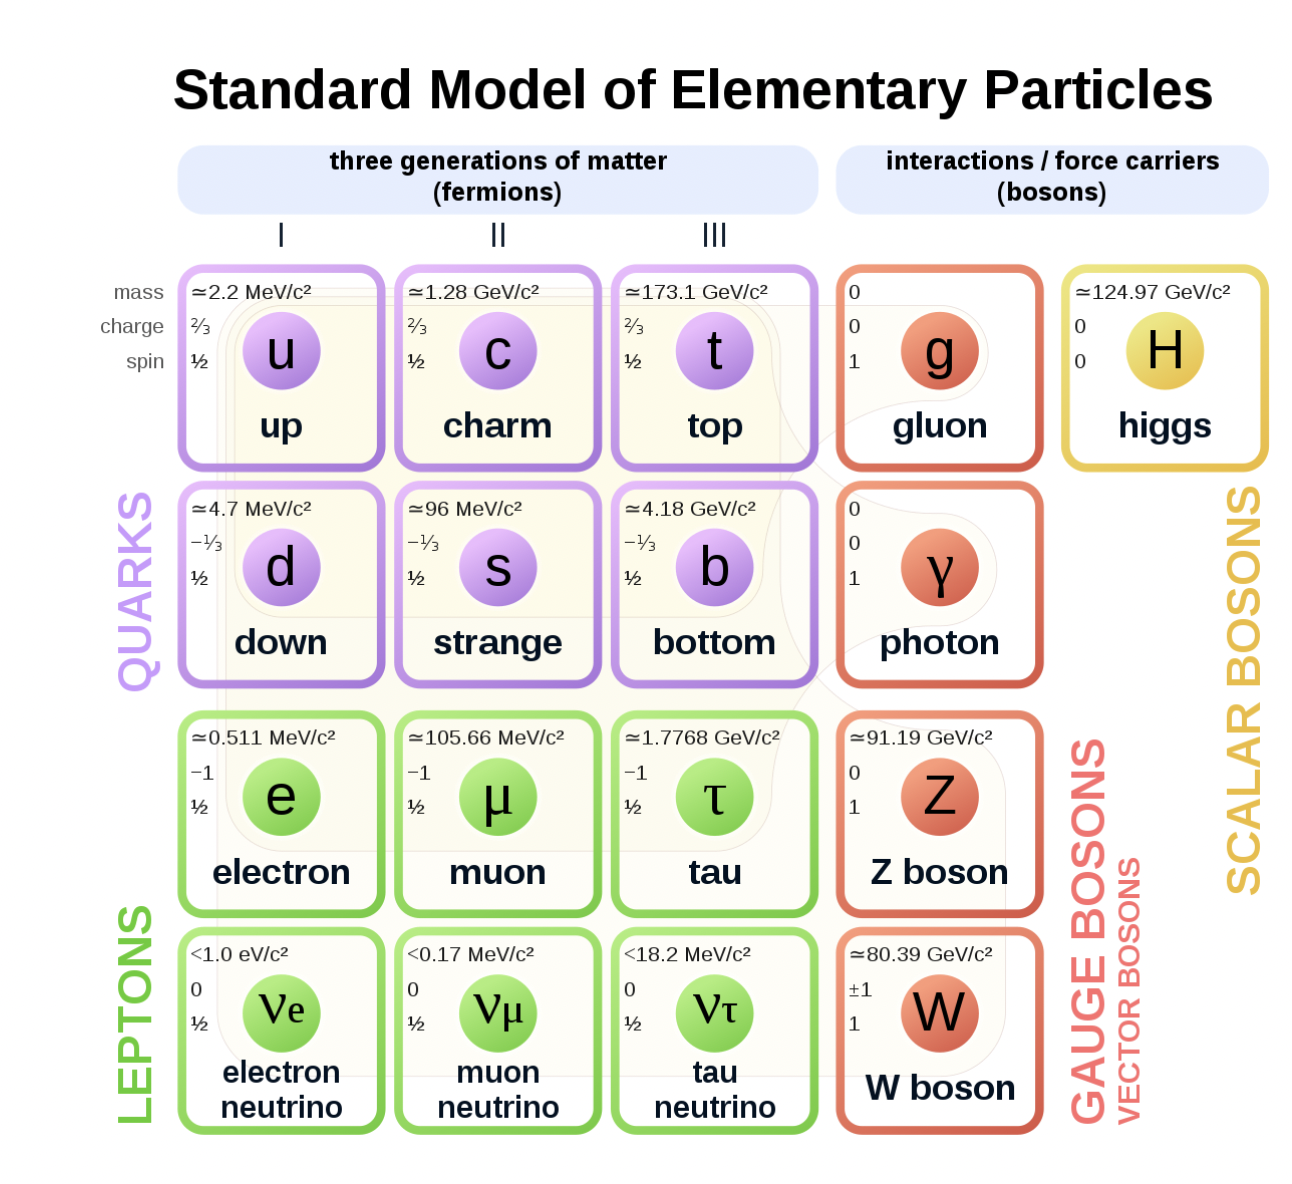
\includegraphics[scale=0.7]{fig/CreativeCommonsSM.png}
    \label{fig:SMTable}
\end{figure}

\begin{figure}[!htbp]
    \centering
    \caption{The Standard Model of Particle Physics depicting the central role of the Higgs Boson~\cite{QuantaMagNewMap}.}
    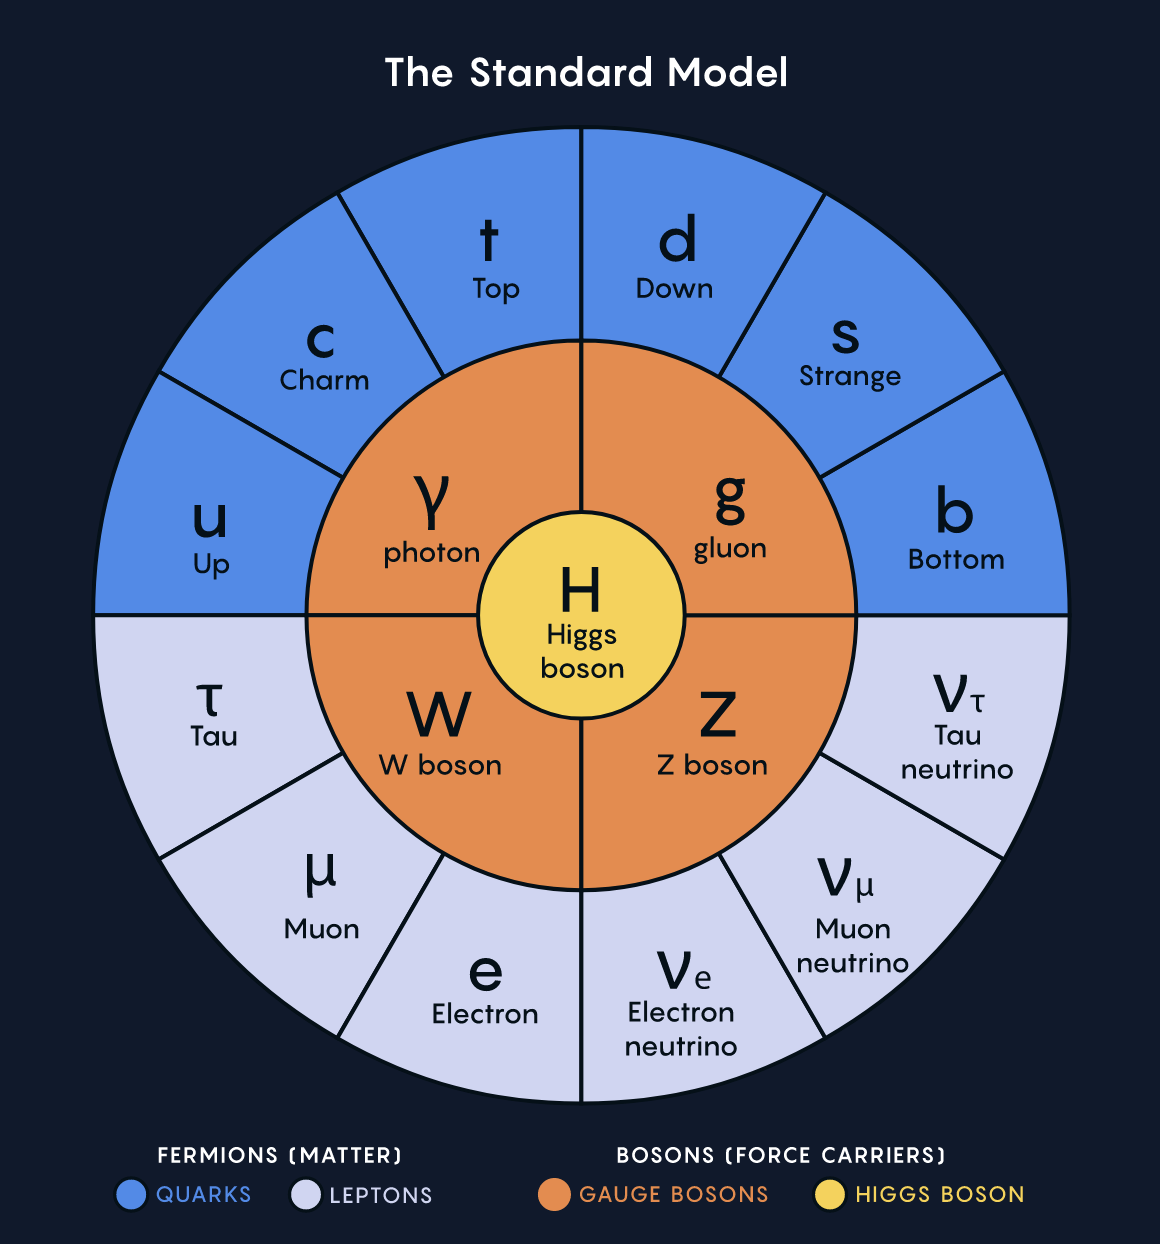
\includegraphics[scale=0.7]{fig/SM.png}
    \label{fig:SMDiagram}
\end{figure}


% \subsection{Rules of Interaction} 

% \begin{figure}[!htbp]
% 	\centering
% % 	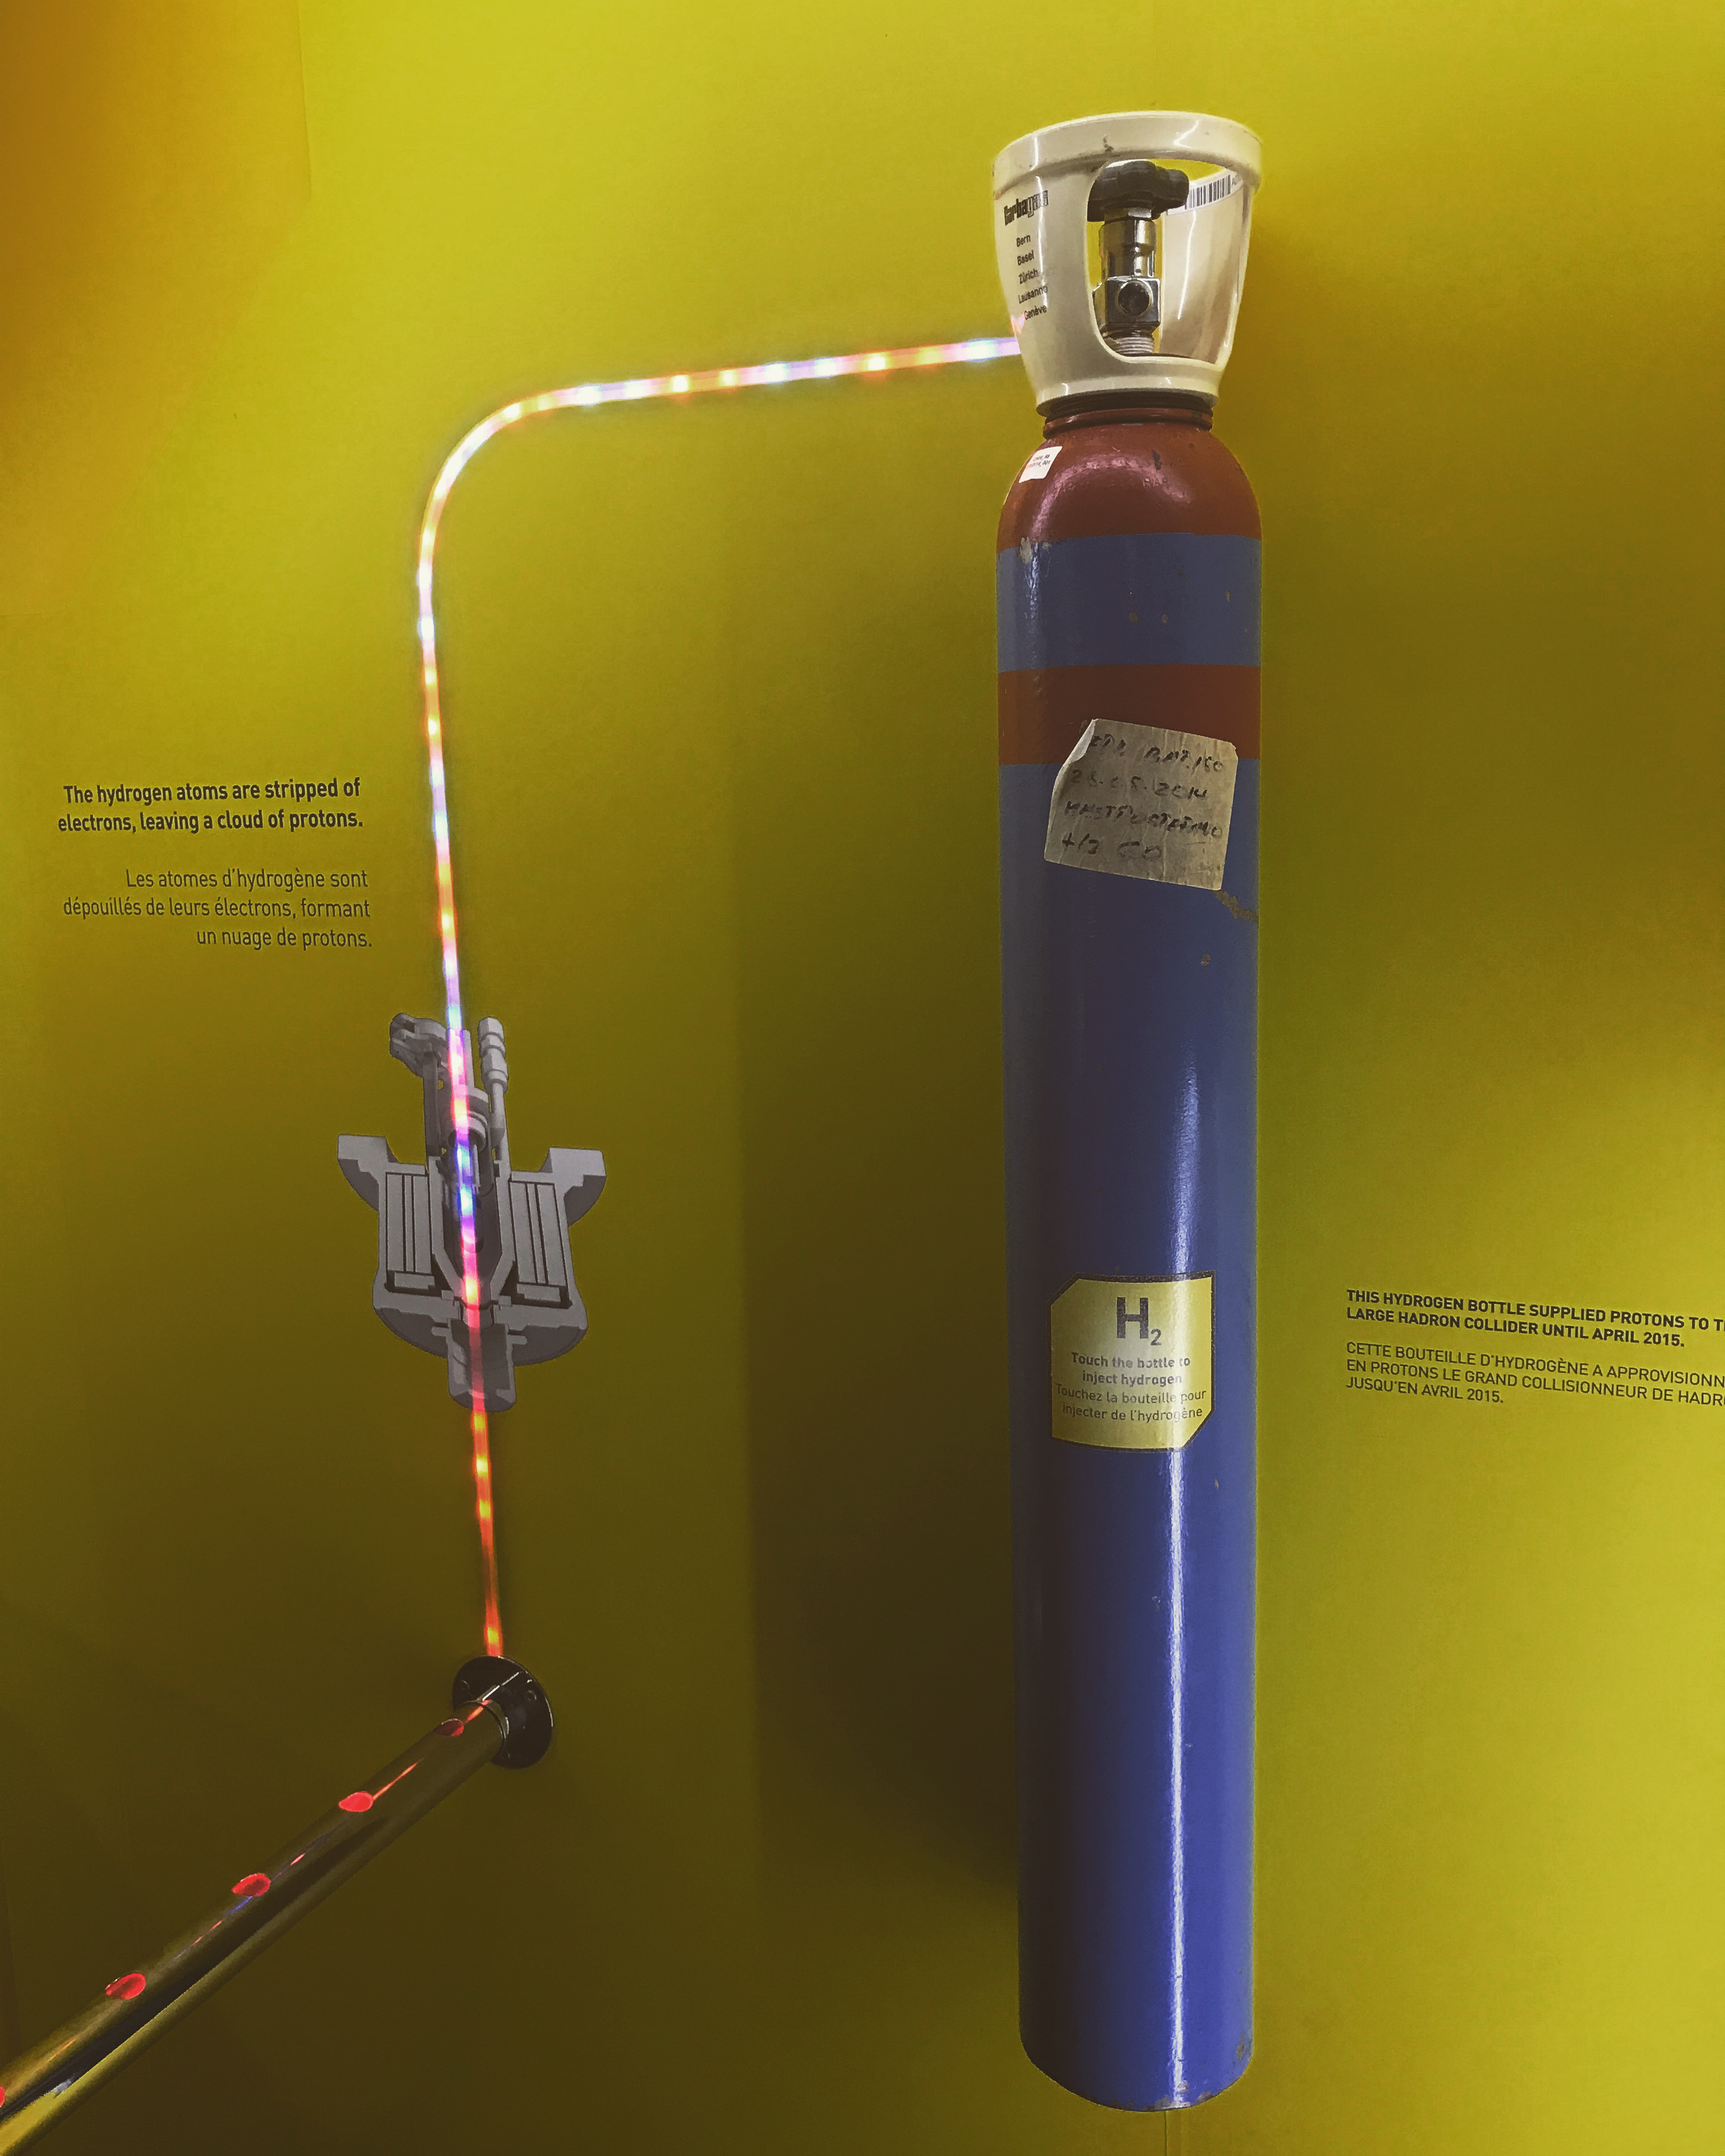
\includegraphics[scale=0.038]{fig/H2Bottle.JPG}
%     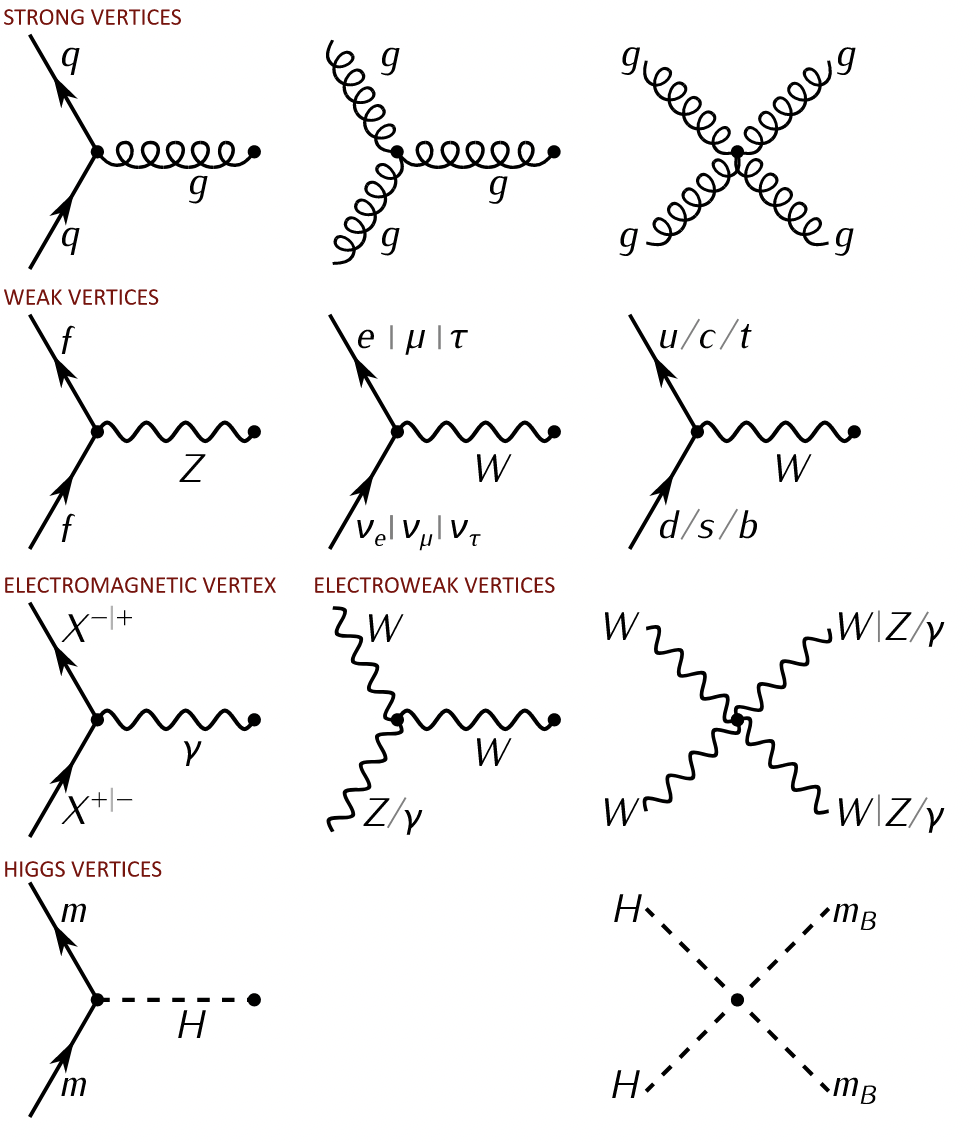
\includegraphics[scale=0.6]{fig/StandardModelOfParticlePhysics.png}
% 	\caption{Fundamental Vertices of the Standard Model. These Feynman diagrams represent the interactions between the fermions and vector gauge bosons in the SM. The W boson charge is determined by the charge of the fermions they interact with and the interaction has to observe the conservation of electric charge.}
% 	\label{fig:FundamentalVertices}
% \end{figure}

% Particle interactions are described intuitively by Feynman diagrams. These Feynman diagrams serve as mathematical book keeping aids which enable physicists to predict the outcomes of particle collision experiments and particle behaviour within the framework of QFT. Each line in a diagram corresponds to a specific particle while the vertices represent the interactions between these particles.

\subsection{QED: Electromagnetic Interaction}
QED or Quantum Electrodynamics is a quantum field theory component of the Standard Model that merges the principles of quantum mechanics with electrodynamics. QED at its core describes the interactions between electrically charged particles via photon exchange and it is described by a basic QED vertex shown in Fig.~\ref{fig:QEDVertex}. 

\begin{figure}[!htbp]
	\centering
    \caption{QED Feynman diagram basic vertex showing an interaction between a fermion and an anti-fermion emitting a photon.}
    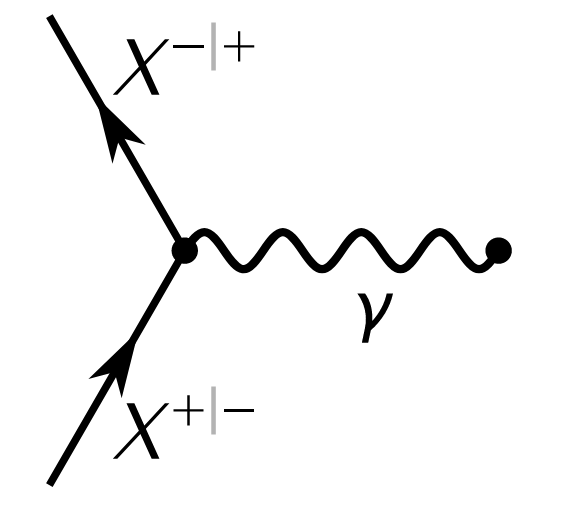
\includegraphics[scale=0.6]{fig/QEDfudnamental.png}
    \label{fig:QEDVertex}
\end{figure}

The fundamental principle of QED revolves around the preservation of electric charge which implies a U(1) symmetry. It is also an example of an abelian gauge theory which is a type of QFT where the gauge transformations commute. 

% The rules of interaction of particles are dictated by symmetry rules governed by the concepts of local and global gauge invariance. From the Lagrangian, $~\mathcal{L}$ the participating quantum fields must obey certain symmetries where the $~\mathcal{L}$ remains invariant under an arbitrary gauge transformation. To illustrate this 

We consider the Lagrangian density of a free Dirac field, $\mathcal{L}_D$ given by:

\begin{equation}
\label{eq:DiracLag}
    \mathcal{L}_{\text{Dirac}} = \bar{\psi}(i\gamma^\mu\partial_\mu - m)\psi. 
\end{equation}

\filbreak
Here, $\gamma^\mu$ are the Dirac matrices, and $\psi$ are the spin-1/2 fields. This Lagrangian has a global $U(1)$ Abelian symmetry, s.t. it remains invariant under this transformation,

\begin{equation}
\label{eq:U1global}
    \psi(x) \rightarrow e^{i\alpha} \psi(x).
\end{equation}

A local transformation on the other hand, where $\alpha$ is replaced with $\alpha(x)$, requires a change in the derivative $\partial_u$ with the covariant derivative defined by
\begin{equation}
\label{eq:CovariantDerivative}
    D_{\mu}  = (\partial_{\mu} - ig A_{\mu}) , 
\end{equation}

where $\partial_{\mu}$ is the partial derivative with respect to the spacetime coordinate $x^{\mu}$, $g$ is the coupling constant, and $A_{\mu}$ is the gauge field. Substituting Eq.~\ref{eq:CovariantDerivative} into Eq.~\ref{eq:DiracLag}, we get a resultant Lagrangian that is invariant under the 

\begin{equation}
\label{eq:AuGaugeTransformation}
   A'_{\mu} = A_{\mu} - \frac{1}{g} \partial_{\mu} \alpha(x), 
\end{equation}

and the local transformation in eq.~\ref{eq:U1global}. Here $A_\mu$ is referred to as the photon field. These steps could be extended to non-Abelian symmetries, where transformation operators do not commute, whose treatment is explained in more detail in standard gauge theory texts such as Ref~\cite{Peskin:1995ev}.

The expression for the QED Lagrangian Density is as follows:

\begin{equation}
\label{eq:QEDLagrangian}
\mathcal{L}_{\textnormal{QED}} = \bar{\psi} (i \gamma^{\mu} \partial_{\mu} - m) \psi - \frac{1}{4} F_{\mu\nu} F^{\mu\nu} - Q \bar{\psi} \gamma^{\mu} \psi A_{\mu},
\end{equation}

where $\psi$ is a fermion field and Q is the electric charge. Each term of the Lagrangian can be understood as the Dirac Lagrangian~\ref{eq:DiracLag} plus the Maxwell's terms plus the fermion field and photon field interaction. This new covariant derivative introduces $A_{u}$ as a new vector field which we we will see as follows is nothing but the electromagnetic four vector potential. Both $A_\mu$ and $D_\mu$ must be invariant under the $U(1)$ transformation as in Eq.~\ref{eq:U1global} and it follows that the commutator of the covariant derivative is also invariant under the same transformation. Expanding the commutator, we find that we can rewrite it in terms of the Electromagnetic field tensor $F^{\mu\nu}$:

% \begin{equation}
% \begin{align*}
%         \label{eq:QEDcommutator}
%     [D_\mu, D_\nu] &= iQ(\partial_\mu A_\nu + A_\mu \partial_\nu - \partial_\nu A_\mu - A_\nu \partial_\mu) \\
%     &= iQ(\partial_\mu A_\nu - \partial_\nu A_\mu) \\ &= iQ$F^{\mu\nu}$ .
% \end{align*}
% \end{equation}

\begin{align*}
    [D_\mu, D_\nu] &= iQ(\partial_\mu A_\nu + A_\mu \partial_\nu - \partial_\nu A_\mu - A_\nu \partial_\mu) \\
    &= iQ(\partial_\mu A_\nu - \partial_\nu A_\mu) \\ 
    &= iQ F^{\mu\nu}.
\end{align*}


We can now write $\mathcal{L}_{QED}$ in the gauge invariant form by substituting the partial derivative with the covariant derivative in Eq.~\ref{eq:CovariantDerivative}.  The QED Lagrangian can be recast simply as:

\begin{equation}
\label{eq:QEDLagrangian}
\mathcal{L}_{\textnormal{QED}} = \bar{\psi} (i \gamma^{\mu} D_{\mu} - m) \psi - \frac{1}{4} F_{\mu\nu} F^{\mu\nu},
\end{equation}

\subsection{QCD: Strong Interactions}

\begin{figure}[!htbp]
	\centering
 	\caption{QCD Fundamental vertices where quark-gluon interactions (left) and gluon self-interactions (middle and right) are shown.}
    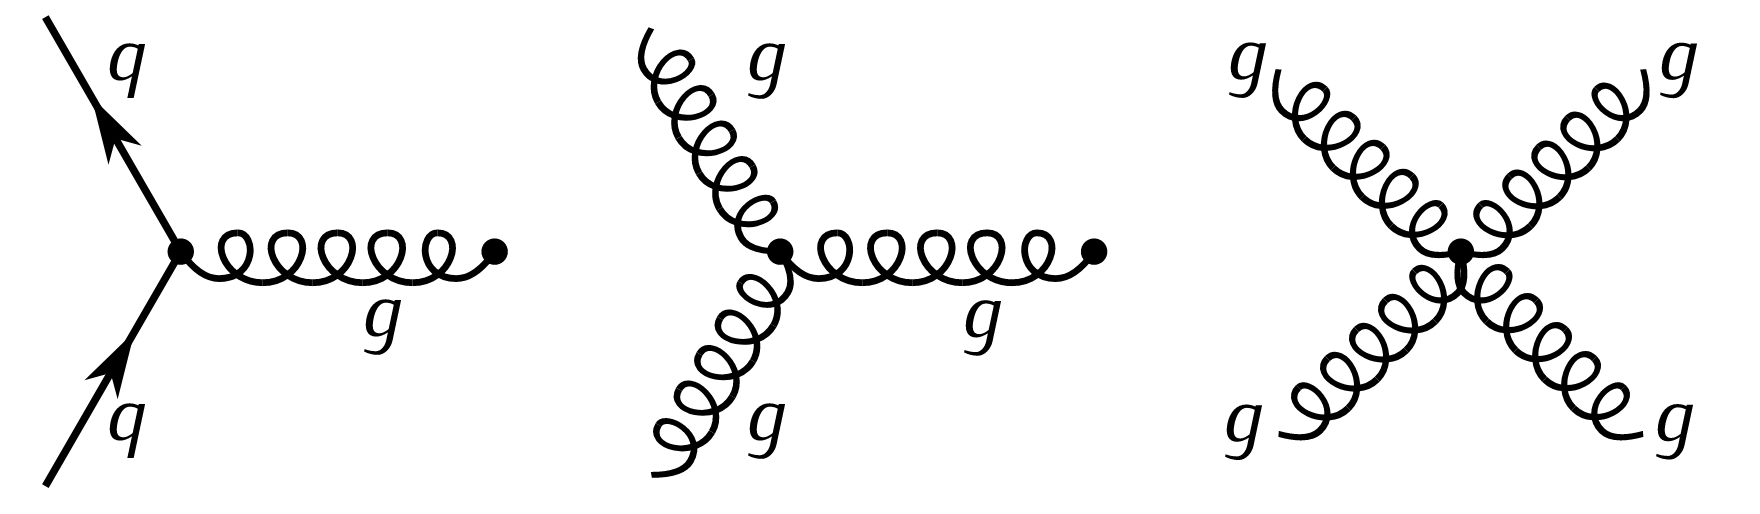
\includegraphics[scale=0.4]{fig/QCDFundamentalVertices.png}
	\label{fig:QCDFundamentalVertices}
\end{figure}

Quantum Chromodynamics (QCD) is the segment within the framework of the Standard model that explains the dynamics of interactions between color-charged particles namely quarks and gluons. This is mathematically captured through transformations within the SU(3) symmetry group to which three distinct charge quantum numbers, namely red, green, and blue are introduced. This stands in stark contrast to QED, which involves a single electric charge. Initial experiments unveiled a crucial aspect of the quantum field theory governing quark interactions - the strength of the interactions decreases as the momentum of the interacting particles escalates. This behaviour is a hallmark of non-Abelian gauge theories of which QCD belongs to. 

The mathematical structure of quantum chromodynamics can be treated as an extension of the idea of local gauge invariance in QED, where the $U(1)$ gauge group as in Eq.~\ref{eq:U1global} is replaced by the $SU(3)$ group of phase transformations on the quark color field: 

\begin{equation}
    \label{eq:QCDgaugeinv}
    q \rightarrow e^{ig_sT^{a}}q,
\end{equation}

where $q$ is the quark field, and $g_s$ is the strong coupling constant. 

QCD is a non-abelian gauge theory due to the non-commutative generators within this group. The generators of the SU(3) group are as follows:

\begin{equation}
    \label{eq:QCDGenerators}
    [T^a, T^b] = if^{abc} T^c
\end{equation}

where $T^{a} = \lambda^{a}/2$, $\lambda^{a}$ are the Gell-Mann matrices and $f^{abc}$ are the structure constants which are antisymmetric coefficients that govern the commutation relations between the Gell-Mann matrices describing how gluons, the force carriers of the strong interaction, interact with each other via the color charges of quarks. The Gell-Mann matrices consist of a collection of eight 3x3 matrices that are Hermitian and have a trace of zero. 

In a similar vein as in Eq.~\ref{eq:AuGaugeTransformation}, we need to introduce the eight gauge fields $G^{a}_{\mu}$, each transforming as:

\begin{equation}
    \label{eq:QCDGauge}
    G^{a}_{\mu} \rightarrow G^{a}_{\mu}' - \frac{1}{g}\partial_{\mu} \alpha_a
\end{equation}

From this we can form a covariant derivative, 
\begin{equation}
    \label{eq:CovariantDerivativeQCD}
    D_\mu = \partial_\mu + igT^{a}G^{a}_\mu.
\end{equation}

This introduces 8 gluon fields, $G^{a}_{u}$, each corresponding to permissible color combinations within the group. Plugging this in the free Lagrangian akin to the Dirac Lagrangian in Eq.~\ref{eq:DiracLag},

\begin{equation}
    \label{eq:FreeLag}
    \mathcal{L} = \bar{q}_{j}(i\gamma^{\mu} \partial_{\mu} - m)q_j, 
\end{equation}

where $q_i$, $i = 1,2,3$ denote the three color fields. The QCD analogue of Eq.~\ref{eq:QEDLagrangian} then becomes, 
\begin{equation}
    \label{eq:FreeLag}
  \mathcal{L} = \bar{q}(i\gamma^{\mu} \partial_{\mu} - m)q - g(\bar{q}\gamma^{\mu}T_{\alpha}q)G^{a}_{\mu}. 
\end{equation}

This is however still not a fully gauge invariant Lagrangian as the last term transformation, since we already from Eq.~\ref{eq:QCDGenerators} that the Gell-Mann matrices don't commute. To mitigate this problem an extra term must be added to Eq.~\ref{eq:QCDGauge}, 

\begin{equation}
    \label{eq:QCDGaugeCorrected}
    G^{a}_{\mu} \rightarrow G^{a}_{\mu} - \frac{1}{g}\partial_{\mu} \alpha_a -f_{abc}\alpha_{b}-G^{a}_{\mu}.
\end{equation}

We then have the final gauge invariant QCD of the form:

\begin{equation}
    \label{eq:QCDLag}
  \mathcal{L} = \bar{q}(i\gamma^{\mu} \partial_{\mu} - m)q - g(\bar{q}\gamma^{\mu}T_{\alpha}q)G^{a}_{\mu} - \frac{1}{4}G^{a}_{\mu\nu}G^{\mu\nu}_{a},
\end{equation}

or in terms of the covariant derivative, 

\begin{equation}
    \label{eq:QCDLag}
  \mathcal{L}_{\textnormal{QCD}} = \bar{q}i\gamma^{\mu} D_{\mu}q - \frac{1}{4}G^{a}_{\mu\nu}G^{\mu\nu}_{a},
\end{equation}

Gluons can directly partake in interactions involving their own color properties. One can expand the QCD Lagrangian~\ref{eq:QCDLag} in terms of the transformation in Eq.~\ref{eq:QCDGaugeCorrected}, and write in symbolic form in terms of increasing orders of ``G"~\cite{Halzen:1984mc},

\begin{equation}
    \label{eq:QCDSymbolic}
  \mathcal{L}_{\textnormal{QCD}} = ``\bar{q}q" + ``G^2" + g``\bar{q}{q}G" + g``G^{3}" + g^2``G^{4}".
\end{equation}

The first two terms describe the free propagation of quarks and gluons. The last three terms are represented schematically in Fig.~\ref{fig:QCDFundamentalVertices}. The first vertex illustrates the interaction between quarks and gluons, while the subsequent two shows 3- and 4-point self-interactions of gluons. 

Gluons' ability to self-interact directly in Quantum Chromodynamics (QCD) results in a significant QCD feature: the strengthening of the coupling between quarks with increasing distance. This phenomenon leads to the preferred formation of new quark-antiquark pairs from the vacuum when attempting to separate bound quarks, causing the creation of two mesons instead of isolated quarks. This confinement of quarks, known as confinement, prohibits the observation of bare quarks in nature, allowing only color-neutral QCD states. Consequences of confinement are evident at high-energy colliders, where high-energy quark or gluon generation results in chains of hadrons forming hadronic jets through fragmentation or hadronization. These jets are pivotal signatures in particle detectors like CMS. At lower energies, scattering interactions lack the energy for jet formation, yielding a spread of hadrons, prevalent in background processes at colliders like the LHC. The top quark, with a short lifetime, decays weakly, sidestepping hadronization, making it a study candidate for ``bare" quarks. Confinement introduces computational challenges, particularly in the non-perturbative QCD regime below the confinement scale, where interaction predictions rely on heuristic tools. Above this scale, asymptotic freedom manifests, with quarks acting as free particles at high energies, valid for hard scattering interactions at colliders through perturbation theory.

\subsection{Electroweak Interactions}

The final piece of the SM, the weak interactions, is an extension of QED which describes how particles charged under weak isospin interact with the $W^{\pm}$ and Z bosons. QED was initially developed to describe the interactions of electrically charged fermions. Following spontaneous symmetry breaking, the photon gains the ability to interact with the electrically charged $W^{\pm}$ bosons as well. Additionally, QED on its own, can function independently as a renormalizable, Abelian gauge theory. However the weak interaction involving the $W^{\pm}$ and Z bosons cannot be adequately described by a standalone gauge theory. It has been determined that these three weak interaction vector bosons and the massless photon in QED need to be collectively addressed within the framework of an $SU(2) \times U(1)$ symmetry in order to explain the observed weak force in the natural world. 

The electroweak theory  has  $SU(2) \times U(1)$ gauge group which have the following fundamental fields: $W^1_{\mu}, W^2_{\mu}, W^3_{\mu}$, associated with the three generators of $SU(2)_{L}$ and $B_{\mu}$, associated with $U(1)_{Y}$. The force mediators, $W^{\pm}$, Z and $\gamma$ are orthogonal combinations of these fundamental fields, which we will show later.

As $SU(2)$ is also a non-Abelian theory, so the weak gauge bosons endowed with charges related to weak isospin, like how gluons bear color charges in QCD. Consequently, they exhibit self-interactions including cubic and quartic couplings of the form $WW\gamma$, $W W Z$, $W W W W$, $W W \gamma\gamma$, $W W ZZ$, and $W W Z\gamma$. The mixing among the original states of $SU(2) \times U(1)$ leads to distinct outcomes that distinguishes the electroweak sector with QCD, the other non-Abelian theory. These unique consequences are essential for aligning theoretical predictions with experimental observations. The theory is also chiral in nature and parity-violating  \cite{Kobayashi:1973fv}., i.e. the symmetry transformations act on ``left-handed" and ``right-handed" fermion fields differently each. This property that the W-boson only couples to fermions of left-handed chirality is a crucial property of the SM and is encoded in the V-A theory\cite{ParticleDataGroup:2018ovx} to explain the the weak nuclear force, which is responsible for processes such as beta decay in atomic nuclei. It is responsible for many of the surprising features of the weak interactions, both the most attractive and the most puzzling ones. 

\begin{figure}[!htbp]
	\centering
% 	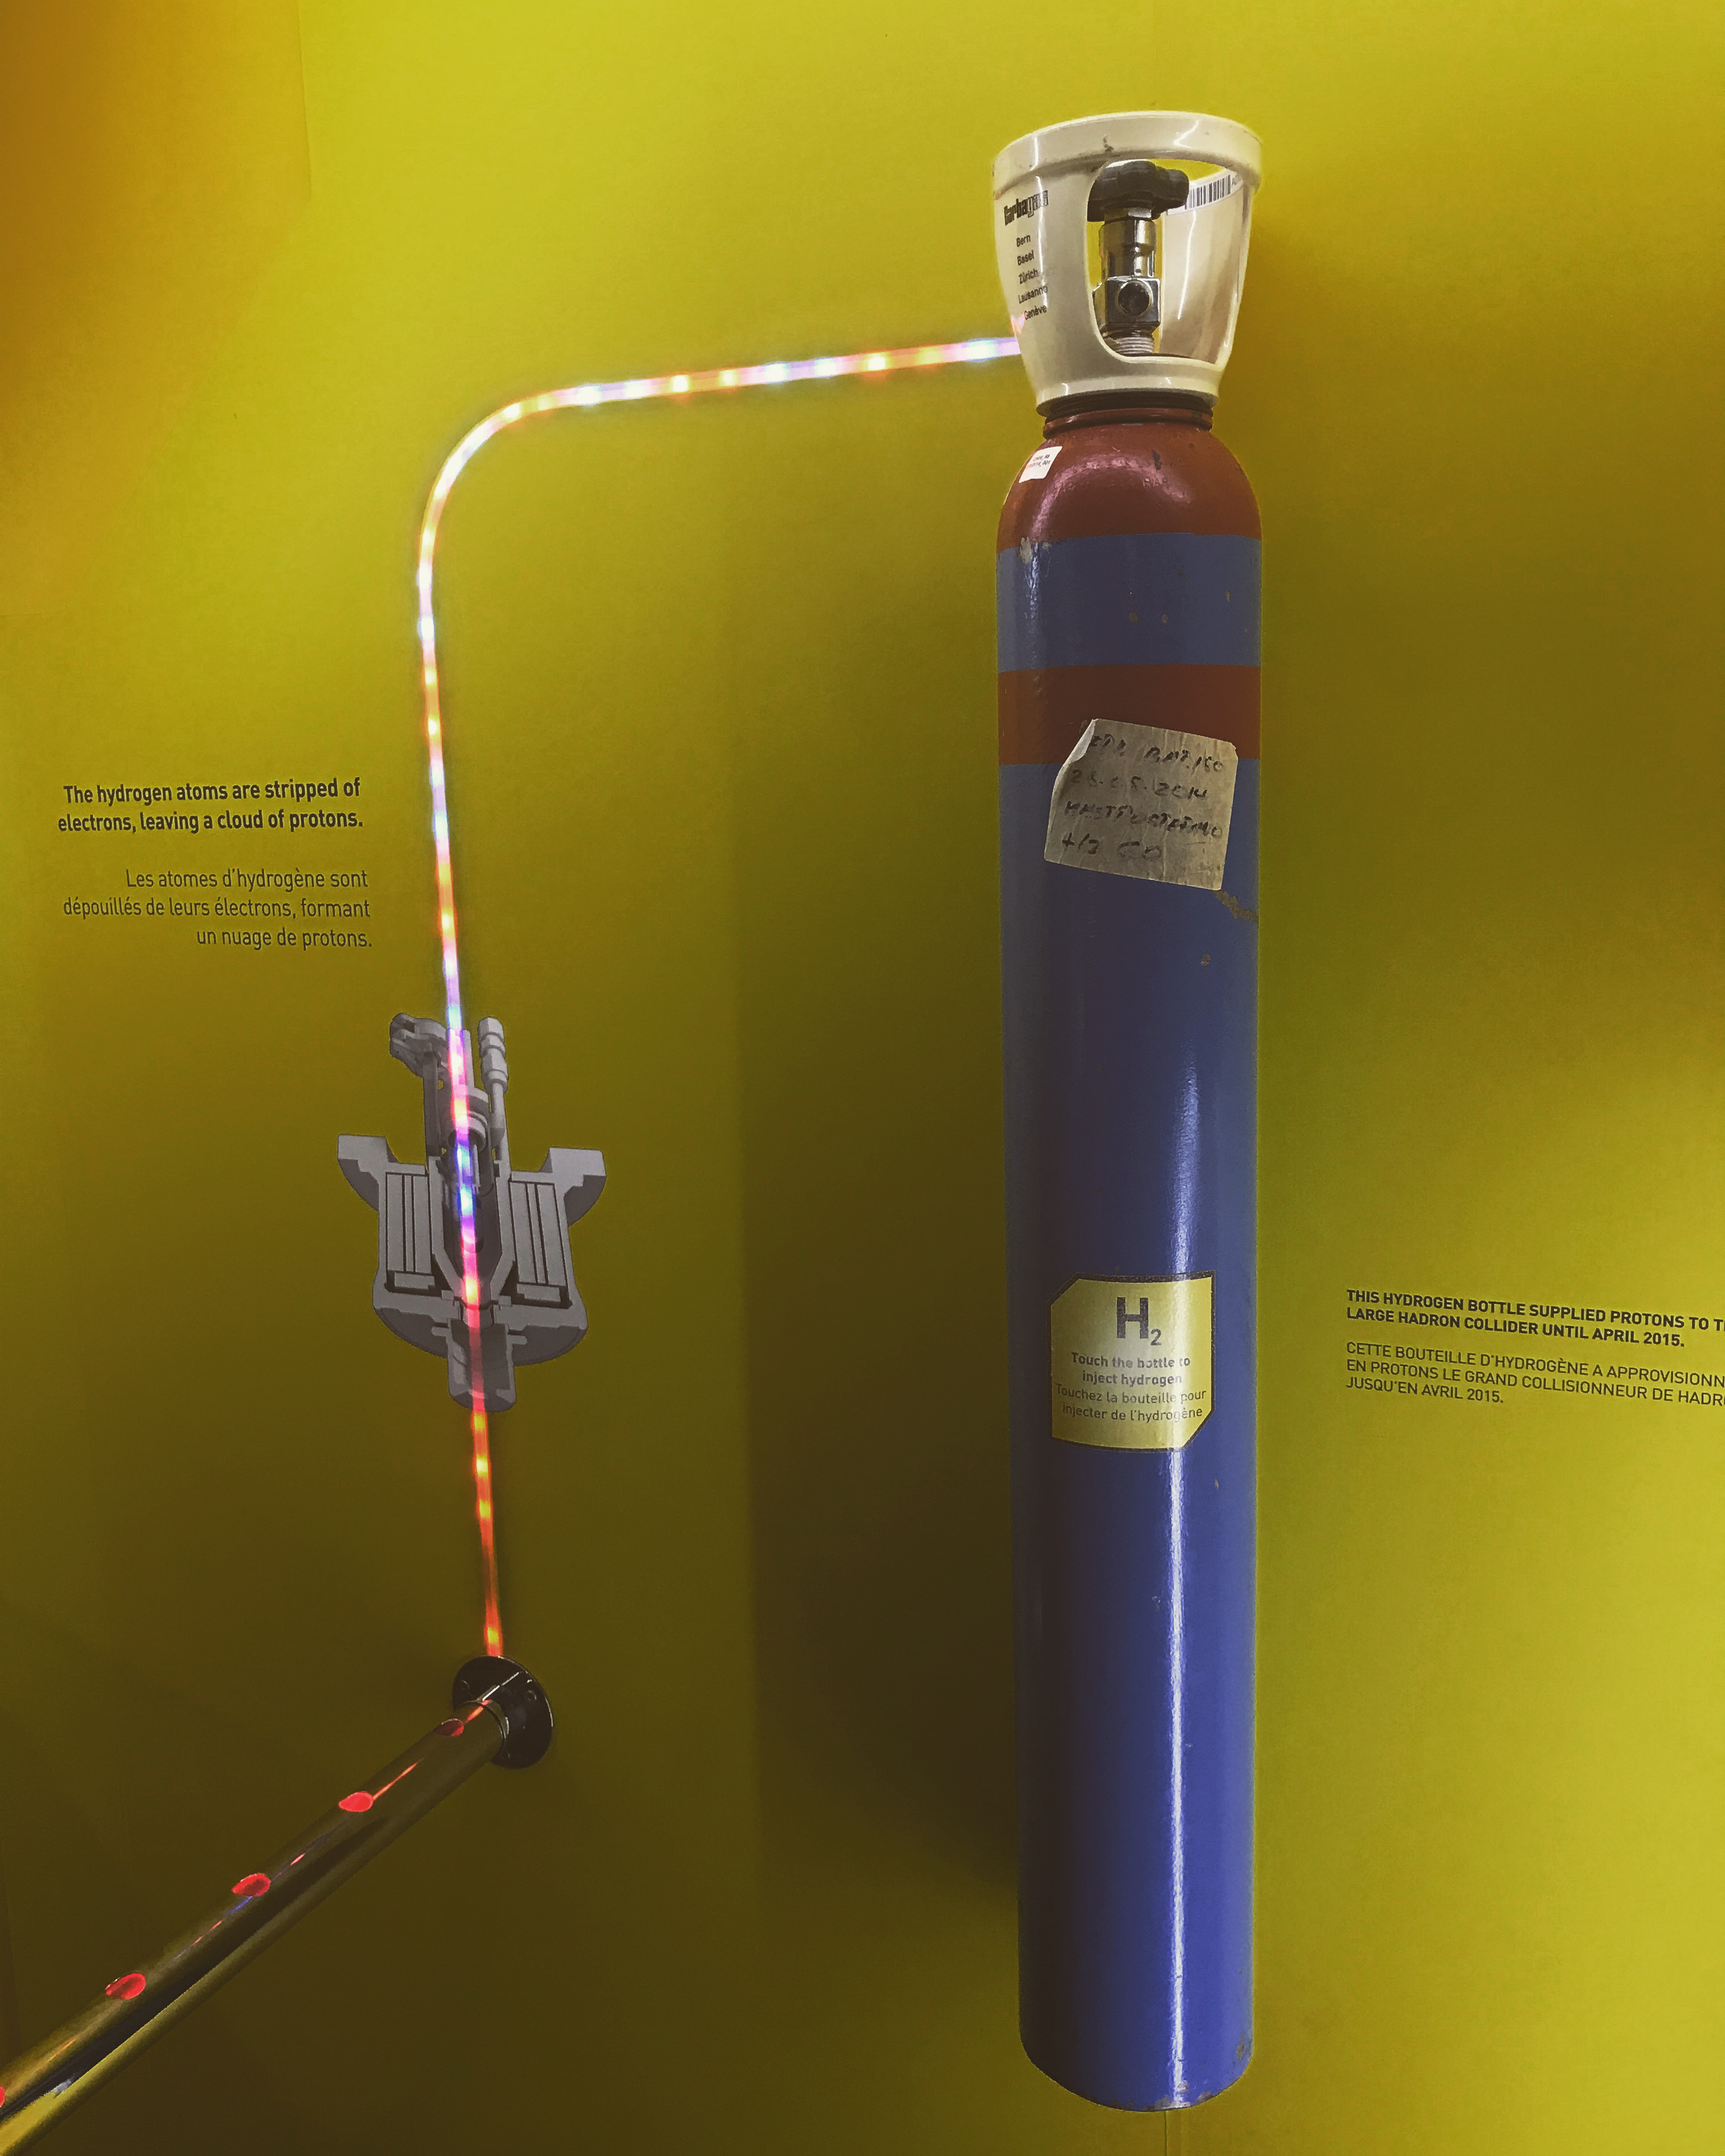
\includegraphics[scale=0.038]{fig/H2Bottle.JPG}
	\caption{Electroweak Interaction Vertices. X are fermions.}
    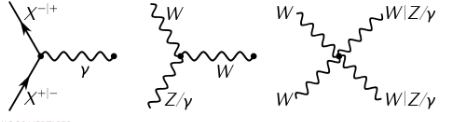
\includegraphics[scale=1.0]{fig/ElectroweakVertices.png}
	\label{fig:Electroweak}
\end{figure}

The mathematical formalism of the electroweak interactions extension of the QED/QCD formalism. To include weak interactions we must write the covariant derivative as:

\begin{equation}
    \label{eq:CovariantDerivativeElectroWeak}
    D_\mu = \partial_\mu - ig_wT^{i}W_{\mu}^{i} - ig_{em}YB_{\mu}, 
\end{equation}

where the operators $T_{i}$ and $\textbf{Y}$ are the generators of the $SU(2)_{L}$ and $U(1)_{Y}$ groups of gauge transformations, respectively. These generators satisfy 

\begin{equation}
    \label{eq:ConservationElectroweakQNum}
   Q = T^3 + \frac{Y}{2}.
\end{equation}
The eigenvalues of these generators, T and Y are also known as the weak isospin and the weak hypercharge quantum numbers. This follows that the electromagnetic current is a combination of the neutral currents and we can write:


\begin{equation}
    \label{eq:ConservationElectroweakCurrent}
   j^{em}_{\mu}= J^3_{\mu} + \frac{1}{2}j^{Y}_{\mu}.
\end{equation}

For the interaction lagrangian, we recall from QED that the interaction is mediated by gauge fields as:

\begin{equation} 
\label{eq:QEDint}
L^{int}_{QED} = -iej^{em}_{\mu} A_{\mu}
\end{equation}

where $j^{em}_{\mu} = \bar{\psi}\gamma^\mu\psi
$ is the $U(1)_{em}$ current and $A_{\mu}$ is the gauge field photon. We copy this for the case of the EW interaction lagrangian and write it in terms of current triplets and singlets

\begin{equation} 
\label{eq:QEDint}
\mathcal{L}^{int}_{EW} = -igj^{i}_{\mu} W^{i\mu} - \frac{ig'}{2} j^{Y}_{\mu} Y^\mu B_\mu
\end{equation}

where the SU(2) part can be expanded as:

\begin{equation} 
\label{eq:SU(2)current}
-igj^{i}_{\mu} W^{i\mu} = -ig\bar{\chi}_L\gamma_{\mu}T\cdotW^{\mu}\chi_{L}
\end{equation}

\begin{equation} 
\label{eq:U(1)}
\frac{ig'}{2} j^{Y}_{\mu} Y^\mu B_\mu = -ig'\bar{\psi}\gamma_{\mu}\frac{Y}{2} \psiB^{\mu}. 
\end{equation}

The vector bosons associated with the particles $W^{\pm}$, Z and $\gamma$, can be constructed as linear combinations of $W^{i}_{\mu}$ gauge field triplet and the singlet $B^{\mu}$. The massive vector boson is written as,

\begin{equation} 
\label{eq:MassiveVecBoson}
W^{\pm\mu} = \frac{1}{\sqrt{2}}(W^{1}_{\mu} \mp iW^{2}_{\mu}).
\end{equation}
The neutral vector bosons $A_{\mu}$ and $Z^{\mu}$ associated with the massless photon and and massive $Z^{0}$ boson are written as follows:

\begin{equation} 
\label{eq:NeutralVectorBosons}
\begin{align*} 
A^{\mu} = B^{\mu}\cos\theta_{w} + W^{3\mu} \sin\theta_{w} ,\\ 
Z^{\mu} = -B^{\mu}\sin\theta_{w} + W^{3\mu} \cos\theta_{w}.
\end{align*}
\end{equation}

Here $\theta_w$ is the ``weak mixing" or ``Weinberg" angle. Substituting the Eqs.~\ref{eq:NeutralVectorBosons} to the electroweak interaction Lagrangian, grouping together terms with $A^{\mu}$ and $Z^{\mu}$\cite{Halzen:1984mc} and using Eq.~\ref{eq:ConservationElectroweakCurrent}, we find that $\theta_w$ can be written as 

\begin{equation} 
\label{eq:weinbergAngle}
e = g\sin\theta_{w} = g'\cos\theta_{w}.
\end{equation}

In practice, $e$, which is the electron charge and $\sin\theta_{w}$ are used as parameters for the standard model to be measured experimentally. Found in the second term with $Z^{\mu}$ is the weak neutral current:
\begin{equation} 
\label{eq:neutralcurrent}
J^{NC}_{\mu} = \frac{g}{\cos\theta_{w}} (j^3_{u} - sin^2\theta_w j^{em}_{\mu}).
\end{equation}


Here we highlight some key aspects of weak interactions. Firstly, we discuss flavor mixing, which is prominent in quarks but absent in leptons. Weak interactions uphold lepton generation conservation, preventing mixing between different lepton generations. For instance, a W boson interacts with an electron and an electron neutrino but not with a muon and an electron neutrino~\cite{MarkusKluteLectures}. 

% Here we highlight a few important things for the weak interactions. First, is the flavor mixing of quarks which does not occur in leptons. The weak interactions respect the lepton generation, such that there is no mixing between generations. A W boson couples to an electron and an electron neutrino, but not to a muon and an electron neutrino

\begin{equation} 
\begin{align*}
\label{eq:CKMMatrix}
        \begin{pmatrix}
        \nu_e \\
        e 
    \end{pmatrix}, 
    \begin{pmatrix}
         \nu_\mu \\
         \mu \\
    \end{pmatrix},
     \begin{pmatrix}
        \nu_\tau \\
        \tau \\
    \end{pmatrix}
\end{align*}
\end{equation}

In contrast, quark generation is not conserved. Instead, we have the quark doublets that participate in the $SU(2)$ symmetry of the charged-current weak interaction are defined as follows:

\begin{equation} 
\begin{align*}
\label{eq:CKMMatrix}
        \begin{pmatrix}
        u \\
        d' 
    \end{pmatrix}, 
    \begin{pmatrix}
         c \\
         s' \\
    \end{pmatrix},
     \begin{pmatrix}
        t \\
        b' \\
    \end{pmatrix}
\end{align*}
\end{equation}

The primed coordinates are given by the relation involving the CKM matrix in Eq.~\ref{eq:CKMMatrix}. This flavor state mixing, non-conservation in the case of quarks is captured in the CKM matrix, denoted as V: 
% \begin{align*}
% \begin{equation} 
% \label{eq:CKMMatrix}
%         \begin{pmatrix}
%         d' \\
%         s' \\
%         b' \\
%     \end{pmatrix} &=
%     \begin{pmatrix}
%          V_{ud} & V_{us} & V_{ub} \\
%          V_{cd} & V_{cs} & V_{cb} \\
%          V_{td} & V_{ts} & V_{tb}
%     \end{pmatrix}
%      \begin{pmatrix}
%         d \\
%         s \\
%         b \\
%     \end{pmatrix}
% \end{equation}
% \end{align*}

\begin{align*}
\begin{pmatrix}
d' \\
s' \\
b' \\
\end{pmatrix} &=
\begin{pmatrix}
V_{ud} & V_{us} & V_{ub} \\
V_{cd} & V_{cs} & V_{cb} \\
V_{td} & V_{ts} & V_{tb}
\end{pmatrix}
\begin{pmatrix}
d \\
s \\
b \\
\end{pmatrix}
\end{align*}~ \label{eq:CKMMatrix}


In this matrix, the elements $V_{ij}$ represent the complex numbers that describe the mixing between different quark flavor states. The indices (i, j) correspond to the initial and final quark flavor states, where ``u" stands for up quark, ``d" for down quark, ``s" for strange quark, ``c" for charm quark, ``t" for top quark, and ``b" for bottom quark. Since this matrix is mostly diagonal, it results in the suppression of couplings between an up-type quark from one generation and a down-type quark from another to the W boson. In the original Standard Model, neutrinos were considered massless, and thus, there was no mixing in the leptonic sector. However, as we now know that neutrinos have mass, one way to account for this is by introducing right-chiral singlets for neutrinos, allowing them to acquire mass in a manner similar to other Standard Model fermions. This introduces a mixing matrix in the leptonic sector known as the PMNS matrix \cite{Maki:1962mu}. 

Historically, the masses of the weak force carriers had been a significant puzzle. The SM of the 1970s or also known as Glashow-Salam-Weinberg theory predicted the existence of the W and Z bosons but did not provide exact predictions of their masses. They were measured later at CERN with the UA1 experiment (W) and the UA2 collaboration (Z-boson). The origin of their masses was elusive and couldn't be incorporated back then into the SM theory in a gauge-invariant matter. This posed as a challenge for achieving true unification. We will see in the next section the significance of the Higgs Mechanism in how particles acquire mass through spontaneous symmetry breaking and preserving the gauge invariance of the theory.



% In contrast, in theories with unbroken symmetries like Quantum Electrodynamics (QED) and Quantum Chromodynamics (QCD), gauge bosons are massless. 
% However, mass terms can be introduced in a gauge-invariant manner when symmetries are broken. Therefore, the symmetry associated with the weak force mediators must indeed be a broken symmetry. The Higgs Mechanism effectively breaks the symmetry of the electroweak $SU(2) \times U(1)$ group while demonstrating how the inclusion of a scalar field preserves the gauge invariance of the theory.

\subsection{Higgs Mechanism and Spontaneous Symmetry Breaking} \label{sec:HiggsMechanism}

The Higgs mechanism was conceived originally to provide mass to the weak gauge bosons. However, it also offers a means of imparting mass to fermions through the Yukawa coupling. We will show both in this section. Consequently, the Higgs boson forms direct connections with all massive particles within the Standard Model. Furthermore, the Higgs boson itself possesses mass, though it is not a gauge boson. It acquires a mechanism for self-interaction through the Higgs potential. The interaction vertices involving the Higgs are illustrated in Figure~\ref{fig:HiggsVertices}. The first of these (Figure 3.6a) delineates the interaction between the Higgs boson and massive particles. 

\begin{figure}[!htbp]
	\centering
    \label{fig:HiggsVertices}
    \caption{Higgs Interaction Vertices.}
    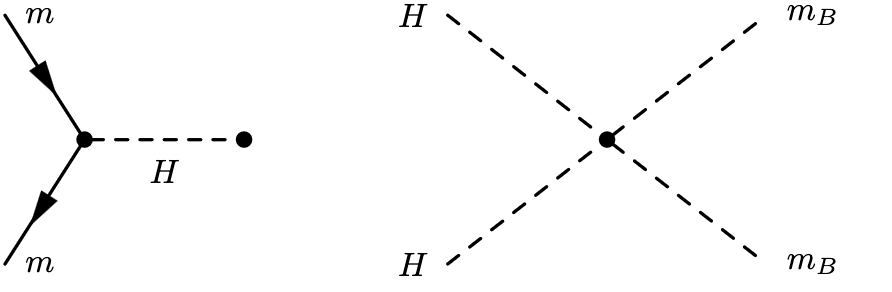
\includegraphics[scale=1.0]{fig/HiggsInteraction.png}
\end{figure}

An ad hoc introduction of vector boson mass terms in the Lagrangian leads to a violation of gauge invariance. For the QED Lagrangian in Eq.~\ref{eq:QEDLagrangian}, a mass term of the form 

\begin{equation}
    \label{eq:AmuWrongMassterm}
    \mathcal{L} = \frac{1}{2}M^2_{A}A^{\mu}A_{\mu}
\end{equation}

would destroy gauge invariance under the transformation of $A_{\mu}$(Eq.~\ref{eq:AuGaugeTransformation}). To generate mass for the gauge bosons, the local gauge symmetries must be broken. 

Standard introductory particle physics texts and lectures~\cite{Halzen:1984mc}
usually begin with a toy model where a single complex scalar field is coupled to the U(1) gauge field 

\begin{equation}
    \label{eq:ToyScalarFieldLagrangian}
    \mathcal{L} = -\frac{1}{4} F_{\mu\nu}F^{\mu\nu} + |D_{\mu}|^2 - V(\phi)
\end{equation}

% (\partial_{\mu}\phi)(\partial^{\mu}\phi) - \frac{1}{2} \mu^2 |\phi|^2 - \lambda |\phi|^4

where $D_\mu = \partial_{\mu} - ieA{\mu}$ and $V =\mu^2 |\phi|^2 - \lambda |\phi|^4 $. For $\mu^2 < 0$, this is just the QED Lagrangian for a charged complex scalar particle of mass $\mu$ save for the $\phi^4$ self-interaction term. It has a unique minimum at zero and does not break the symmetry. To generate the mass terms we take $\mu^2 > 0$. This breaks the $U(1)$ symmetry and has a minimum at 

\begin{equation}
    \label{eq:Minimum}
    <\phi> = \frac{v}{\sqrt{2}} = \sqrt{-\frac{\mu^2}{2\lambda}}.
\end{equation}
This is a circle of minimum with radius $v$ and is shown in Fig.~\ref{fig:MexicanHat}. 

For convenience we can rewrite $\phi$ in terms of real fields, 

\begin{equation}
    \label{eq:RealFields}
    \phi = \frac{v+h}{\sqrt{2}}e^{i\frac{\theta}{v}},
\end{equation}

here $h$ and $\chi$ are the Higgs and Goldstone bosons respectively

\begin{align}
\label{eq:HiggsGoldstone}
    L = &-\frac{1}{4} F_{\mu\nu} F^{\mu\nu} - e v A_\mu \partial^\mu \chi + \frac{e^2 v^2}{2} A_\mu A^\mu \nonumber \\
    &+ \frac{1}{2} (\partial_\mu h \partial^\mu h - 2\mu^2 h^2) \nonumber \\
    &+ \frac{1}{2} \partial_\mu \chi \partial^\mu \chi + \textnormal{interaction terms}. \label{eq:HiggsGoldstone}
\end{align}


With this new Lagrangian, the photon is imparted a mass $m_A = ev$. The theory now has a Higgs boson $h$ of mass $m_h = \sqrt{2\mu} =\sqrt{2\lambda v^2} \lambdav$, and a massless Goldstone $\theta$. If we choose the following gauge transformation:

\begin{equation}
\label{eq:GoldstoneGauge}
A_{\mu} \rightarrow A_{\mu} + \frac{1}{ev}\partial_{\mu}\theta
\end{equation}

the theory will be independent of $\theta$. The theory will not just have two interacting massive particles which are $A_\mu$ and $h$. 

The procedure could be generalized for an $SU(n)$ gauge symmetry~\cite{MarkusKluteLectures}. 

\begin{equation}
\begin{split}
\label{eq:SU(N) higgs}
    \mathcal{L} &= D_{\mu}\phi^{\dagger}D^{\mu}\phi - V(\phi) \\
     V(\phi) &= \mu^2\phi^{\dagger}\phi + \lambda(\phi^{\dagger}\phi)^2
\end{split}
\end{equation}

This is invariant under the following transformations:

\begin{equation}
\begin{split}
\label{eq:SU(N)transformation}
    \phi_{i} &\rightarrow (1-\epsilon^{a}\tau^{a})_{ij} \phi_j\\
    D_{\mu} \phi &= (\partial_{\mu} - ig\tau^aA^a_{\mu})\phi 
\end{split}
\end{equation}

where $i, j= 1, 2,...,n; a = 1, ..., n^2 -1$, $g$ is a coupling constant, and $\epsilon^a$ are small parameters and $\tau^a$ are the group generators of the theory. 

Now that the concept of spontaneous symmetry breaking is introduced, we can introduce the Weinberg formulation for a Higgs Lagrangian, similar to Eq.~\ref{eq:SU(N) higgs} such that the $W^{\pm}$ and $Z$ bosons are massive and the photon remains massess. Here we introduce four real scalar fields which is equivalent to a Higgs $SU(2)$ doublet:

\begin{equation}
\phi = \begin{pmatrix}
        \phi^+\\
        \phi^0
        \end{pmatrix}
    = \frac{1}{\sqrt{2}}\begin{pmatrix}
        \phi_1 + i \phi_2\\
        \phi_3 + i \phi_4.
        \end{pmatrix}
\end{equation}

The covariant derivative would have the form:
\begin{equation}
\label{eq:HiggsCov}
D_{\mu} = \partial_\mu - i\frac{g}{2}\sigma^aW^a_{\mu}-i\frac{g'}{2}B_\mu,
\end{equation}
which indicates a coupling of the Higgs to SU(2) gauge bosons, $W^a, a= 1,2,3 $ and the $U(1)$ gauge boson, B. Once again, $\mu^2 < 0$ for spontaneous symmetry breaking to occur, with the following choice of a minimum or vacuum expectation value (VEV):

\begin{equation}
\label{eq:VEV}
<\phi> = \phi_0 = \frac{1}{\sqrt{2}}\begin{pmatrix}
         0 \\
         v
        \end{pmatrix}.
\end{equation}

Substituting this vacuum expectation value~Eq.~\ref{eq:VEV} to the Lagrangian in Eq.~\ref{eq:SU(N) higgs}, 

\begin{equation}
\label{eq:MassesLagrangian}
D_{\mu}\phi^{\dagger}D^{\mu}\phi  = (\frac{1}{2}vg)^2W^+_{\mu}W^{-\mu} + \frac{1}{8}v^2 (W^3_{\mu}, B_{\mu})\begin{pmatrix}
    g^2  & -gg' \\
    -gg' & g'^2
\end{pmatrix}
\begin{pmatrix}
    W^{3\mu} \\
    B^{\mu}
\end{pmatrix}.
\end{equation}

Multiplying the matrices, and identifying the mass terms, we have:

\begin{equation}
\label{eq:BosonMasses}
\begin{aligned}
M_w &= \frac{gv}{2}, \quad &W^{\pm}_{\mu} &= \frac{1}{\sqrt{2}}(W^1_{\mu} + W^2_{\mu}) \\
M_z &= \frac{v}{2}\sqrt{g^2+g'^2}, \quad &Z_{\mu} &= \frac{gW^3_{\mu} - g'B_{\mu}}{\sqrt{g^2+ g'^2}} \\
M_A &= 0, \quad &A_{\mu} &= \frac{g'W^3_{\mu} + gB_{\mu}}{\sqrt{g^2+ g'^2}}.
\end{aligned}
\end{equation}

If we reexpress the results here with the weak mixing angle in eq.~\ref{eq:weinbergAngle}, we can relate the $W^{\pm}$ and Z masses with

\begin{equation}
    \frac{M_{W}}{M_{Z}} = \cos\theta_{W}.    
\end{equation}
Experimentally, the masses are measured to be,
\begin{equation}
\begin{align}
    M_W \approx 81 GeV \\
    M_Z \approx 93 GeV,
\end{align}
\end{equation}

which are in impressive agreement with the predictions of SM.

% \quad \textnormal{with}

\begin{figure}[!htbp]
	\centering
% 	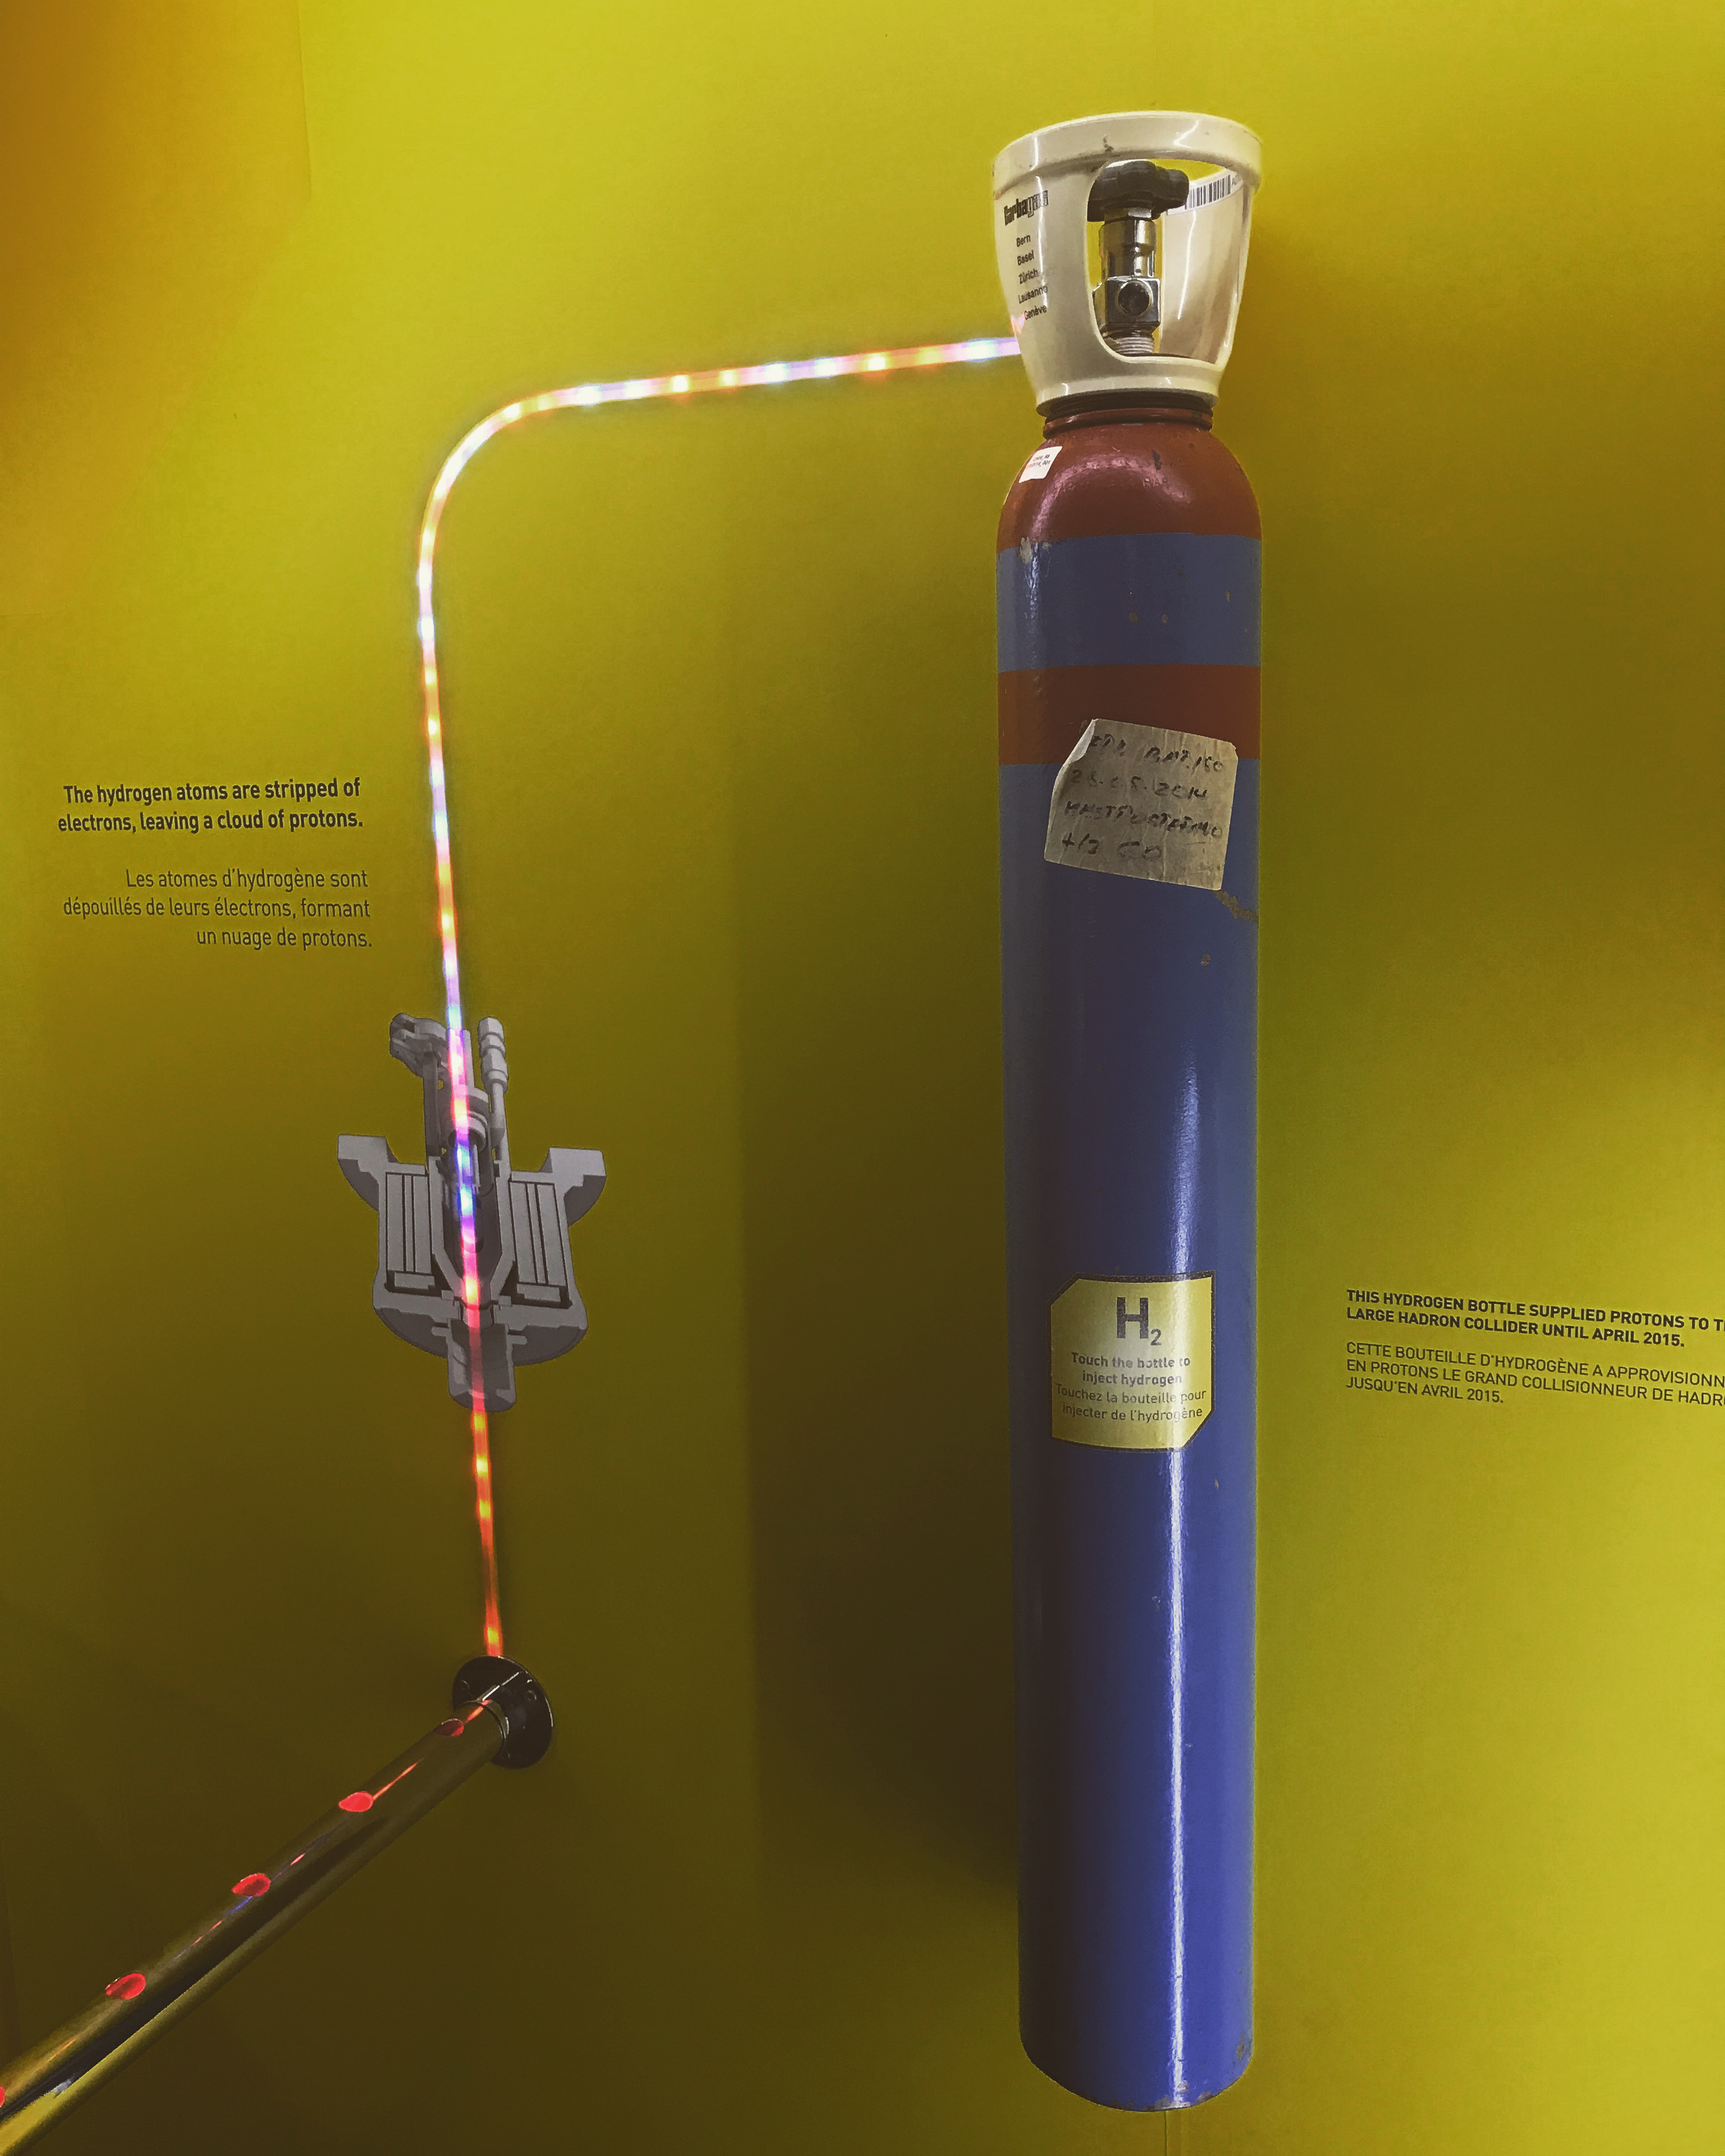
\includegraphics[scale=0.038]{fig/H2Bottle.JPG}
	\caption{The infamous ``Mexican Hat" Higgs potential for the case of $\mu^2 <0$ and $\lambda >0$. There is a circle of minima of radius v.}
    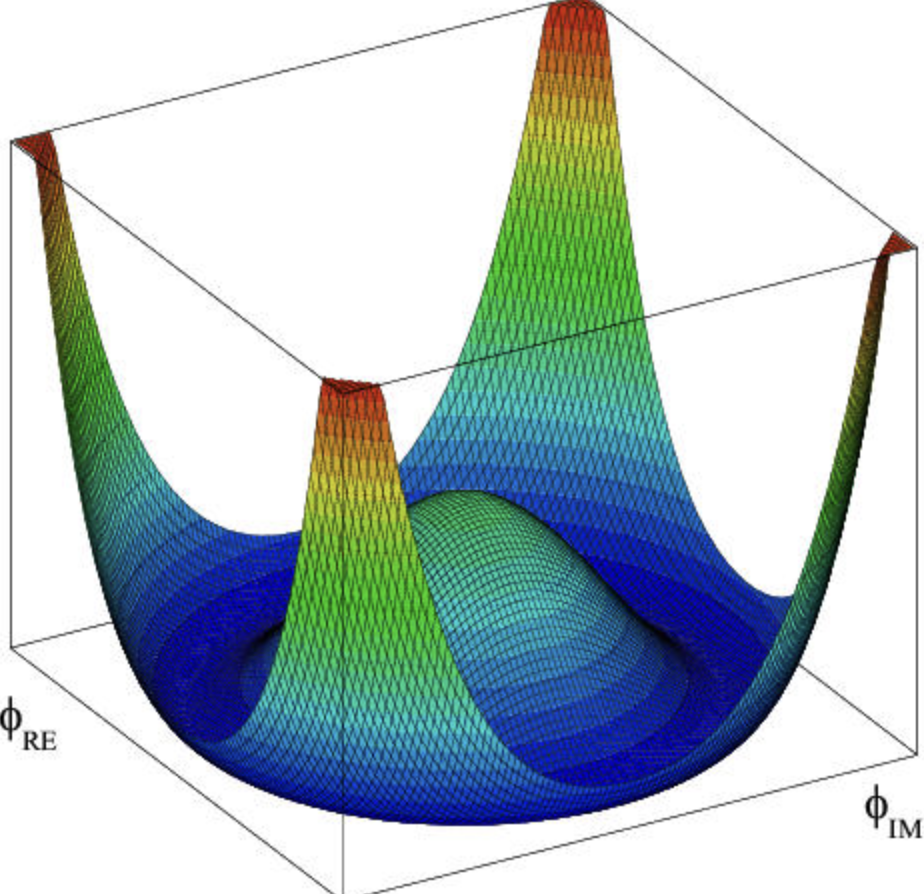
\includegraphics[scale=0.5]{fig/MexicanHat.png}
	\label{fig:MexicanHat}
\end{figure}

As mentioned earlier, the fermions gain mass via the Yukawa coupling of the single Higgs doublet $\phi$ with the fermions~\cite{Nguyen:HiggsMechanism}. In a nutshell, one can write a Yukawa coupling term in the lagrangian for a fermion:

\begin{equation}
    \label{eq:YukawaCouplingLag}
    \mathcal{L}_{\text{Yukawa}} = -g_f\bar{\psi_f} \phi \psi_f + h.c. 
\end{equation}

where g is a dimensionless coupling constant for some fermion $f$, $\psi_f$ is the fermion field and $\phi$ is the Higgs field. After spontaneous symmetry breaking, the Higgs field takes on the vacuum expectation value in Eq.~\ref{eq:VEV} the Lagrangian in Eq.~\ref{eq:YukawaCouplingLag}. For illustration, we do this for the first generation of fermions:

\begin{equation}
    \label{eq:YukVEV}
    \mathcal{L}_{\text{Yukawa}} =  \frac{f_e v}{\sqrt{2}} \left( \bar{e}_L e_R + \bar{e}_R e_L \right) + \frac{f_u v }{\sqrt{2}} \left( \bar{u}_L u_R + \bar{u}_R u_L \right) +  \frac{f_d v}{\sqrt{2}} \left( \bar{d}_L d_R + \bar{d}_R d_L \right), ...
\end{equation}
From here one can read off the masses as:
\begin{equation}
    \label{eq:FermionMasses}
   m_i = \frac{f_iv}{\sqrt{2}}, \quad i = e, u, d.
\end{equation}

One thing to note is that the neutrinos do not have right-handed partners in the SM and therefore could not acquire a mass term through Yukawa coupling \cite{Martin:1997ns}. 

On July 4, 2012, the CMS and ATLAS experiments independently announced the discovery of a particle consistent with the Higgs boson. This landmark achievement, while significant, did not ``complete" the Standard Model in the sense of resolving all fundamental questions in particle physics. Rather, it confirmed one of the final pieces of the SM puzzle, highlighting that numerous unresolved questions and challenges remain which requires further the exploration of new theoretical frameworks to expand our understanding of the universe.

\section{Limitations of the Standard Model}~\label{sec:SMLimitations}
In this section, we briefly give an itemized overview of a number of open questions in the Standard Model and discuss in more detail how the BSM models we are exploring play a role in addressing these open problems. 
\begin{itemize}
    \item  \textbf{Hierarchy Problem}: The Standard Model struggles to explain the vast disparity in the strengths of the fundamental forces, particularly why gravity is incredibly weaker than the other forces in our four-dimensional spacetime.
    \item \textbf{Parameter Fine-tuning}: The Standard Model involves several ``unnatural" parameters, such as the low mass of the Higgs boson. Adjusting these parameters to match experimental observations appears contrived, lacking a deeper theoretical explanation.
    \item  \textbf{Quantum Theory of Gravity}: While the Standard Model successfully describes the other fundamental forces through quantum field theories, it falls short in providing a consistent quantum field theory for gravity, a long-standing challenge in theoretical physics.
    \item \textbf{Dark Matter and Dark Energy}: The Standard Model accounts for only a tiny fraction, approximately 4$\%$, of the total matter-energy content of the universe. It fails to address the presence of dark matter and the mysterious dark energy, both of which dominate the universe's composition.
    \item \textbf{Baryon Asymmetry}: There is an unexplained imbalance between matter and antimatter in the universe, known as the baryon asymmetry, which the Standard Model does not elucidate.
    \item \textbf{Strong CP Problem}: The mathematical formulation of Quantum Chromodynamics (QCD) within the Standard Model predicts a violation of CP-symmetry in strong interactions, which contradicts experimental observations. CP-symmetry dictates that the laws of physics should remain unchanged when particles are replaced with their antiparticles (charge reversal), followed by a left-right flip (parity reversal).
    \item \textbf{Neutrino Masses}: Neutrinos, initially assumed to be massless in the Standard Model, have been observed to have tiny but non-zero masses through experimental evidence. The SM does not naturally incorporate these neutrino masses and mixing angles, necessitating an extension of the theory to accommodate them.
    
\end{itemize}

\subsection{Hierarchy and Naturalness}~\label{sec:HierarchyandNaturalness}
It is well-established at this point that the Standard Model is a work-in-progress specially at higher energy regimes. Extensions to the standard model are guided by the principle of the desert hypothesis which has the fundamental premise that there is no new physics between the electroweak unification scale at $m_{EW}\approx1$~TeV and near the Planck mass or the reduced Planck Scale $M_P\approx 10^{18}$~GeV where quantum gravitational effects become significant. This large gap between the two scales refers to the well-known ``hierarchy problem". 

Theorists however think that this desert, 16 orders of magnitude wide, might conceivably host a plethora of successive layers of new effective field theories (EFTs). Among these are the ADD Large Extra Dimensions~\ref{sec:ADDmodel}, the Clockwork Model~\ref{sec:CWmodel} and the Unparticles~\ref{sec:UnparticlesModel}, which could serve diverse purposes, including the initiation of dynamical symmetry breakings or providing explanations for the intricate patterns observed in fermion masses and mixings \cite{Arkani-Hamed:1998jmv}. While the hierarchy problem might not be a direct issue with the Standard Model it reflects unsettling consequences related to the "naturalness" of the Higgs mass. 

The Higgs boson, being the only scalar particle in the Standard Model, possesses a distinct property: its quantum corrections are quadratically sensitive to high energy scales. This issue arises from the substantial quantum corrections originating from the virtual effects of every particle or phenomena directly or indirectly that couples to the Higgs field \cite{Martin:1997ns}. The general form for the Higgs boson mass calculation is written as:

\begin{equation}
    \label{eq:HiggsMass}
    m^2_H = m^2_{bare} + \Delta m^2_{H}, 
\end{equation}

\begin{figure}[!htbp]
	\centering  
    \caption{One-loop quantum corrections to the square of the Higgs mass parameter ($m^2_{H}$) due to a Dirac fermion $f$ in (a), and a scalar (b) $S$ \cite{Martin:1997ns}. }
    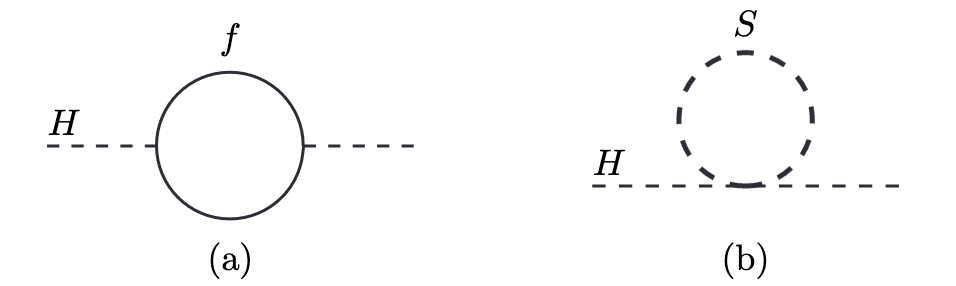
\includegraphics[scale=1.0]{fig/LoopCorrHiggs.png}
	  \label{fig:HiggsQuantumCorr}
\end{figure}

where $m_H$ is the Higgs boson mass measured to be $125$~GeV, $m_{bare}$ is the Higgs boson bare mass, and $\Delta m^2_{H}$ are the said quantum corrections. To illustrate the problem, consider a correction from a loop described by the Feynman diagram in Fig.~\ref{fig:HiggsQuantumCorr} containing a Dirac fermion of mass $m_f$ coming from a term in the lagrangian $-\lambda_fH\bar{f}f$, 

\begin{equation}
    \label{eq:HiggsMass}
    \Delta m^2_{H} = - \frac{|\lambda_f|^2}{8\pi^2} \Lambda^2_{\textnormal{cutoff}} + ...
\end{equation}

Here, $\Lambda_{\textnormal{cutoff}} = \Lambda_{UV}$ refers to the ultraviolet momentum cutoff that is used to regulate the loop integral. It is also the energy scale at which new physics emerges. We can surmise that the SM is an EFT or a low-energy QFT approximation of some higher-energy theory which may include gravity and it is valid up to some cutoff scale. When bridging the hierarchy gap, $\Lambda_{\textnormal{cutoff}} \rightarrow \Lambda_{Planck}$, this contribution becomes too large, notwithstanding that these contributions add up for each fermion in the SM. At the $\Lambda_{Planck}$ scale, the bare mass and the quantum corrections would need to cancel over 30 orders of magnitude to match the measured value of the Higgs at 125 GeV. It seems that these quantum corrections have to be finely tuned and canceled out with an incredible degree of precision. This fine-tuning seems unnatural because it suggests that the observed Higgs mass is a delicate balance between the tree-level mass and the quantum corrections. In other words, it appears unlikely that nature would naturally set the Higgs mass to this specific value, given the sensitivity of the corrections to it. This is known as the Higgs naturalness problem.

\section{Beyond Standard Model Non-resonant Signals}~\label{sec:BSMNonReso}
The hierarchy and naturalness problem necessitated extensions to the Standard Model of which the primary and uncontested early candidate was Supersymmetry (SUSY). SUSY posits the existence of yet-to-be-discovered fermionic (bosonic) superpartners to the known bosons and fermions. With this framework, the strong, electromagnetic and weak coupling constants could be extrapolated and converge at a point just below the Planck Scale \cite{Martin:1997ns}.

In 1998, authors Nima Arkani-Hamed, Savas Dimopoulos, and Georgi Dvali (ADD), proposed a new framework\cite{Arkani-Hamed:1998jmv, Arkani-Hamed:1998sfv} that has a diametrically opposing premise from SUSY. They asserted that there is no desert between the electroweak scale and the Planck scale. Instead, they hypothesize the existence of additional $n_{ED}$ spatial dimensions with a radius $R$ which modifies the fundamental Planck Scale, which transforms the fine-tuning dilemma into a question of dynamics and geometry \cite{5LittleStringTheoryAtATeV}. With this approach, they also showed that the weakness of gravity could be explained by the existence of these extra dimensions in which only gravity propagates. Additionally, it has been shown~\cite{Dienes:1998vg, Dienes:1998vh} that these extra dimensions naturally lead to the unification of the coupling strengths at scales substantially below the usual GUT/ Planck scale. 

The idea of extra spatial dimensions is not entirely new. It has a historical precedent dating back to the 1920s, notably explored by Kaluza and Klein as an attempt to unify the fundamental forces~\cite{Kaluza:1921tu, Klein:1926fj, Klein:1926tv}. In the 1980s, string theory revisited this concept as a requirement for a consistent theory of quantum gravity, with the dimensions compactified near the Planck scale and therefore not testable experimentally ~\cite{ParticleDataGroup:2020ssz}. While the initial endeavour faltered, the Kaluza-Klein (KK) formalism remains valuable today, albeit with modified forms and assumptions. 

A year after the ADD model was proposed, Randall and Sundrum introduced a groundbreaking approach wherein the extra dimension has a warped geometry in a five-dimensional negatively curved, Anti-de Sitter (AdS) spacetime, with a compactification scale near 1/TeV. This model explained the electroweak scale's smallness relative to the Planck scale by invoking a gravitational redshift factor that is intrinsic to the warped AdS metric. Initially conceived for gravity alone, it was soon evident that the Standard Model's gauge fields and fermions could also propagate within these five-dimensional spacetime regions~\cite{Randall:1999ee, Randall:1999vf, ParticleDataGroup:2020ssz}. 

Around a decade later, additional frameworks that try to solve the hierarchy problem through various geometries and or field dynamics were proposed. One model is the Continuum Clockwork Model~\cite{2Clockwork} which has a remarkable resemblance to the Linear Dilaton theory of Little String Theory~\cite{5LittleStringTheoryAtATeV}. At some limit, we show that it is equivalent to the ADD LED and the RS model. Another is the Unparticles Scenario which explores the possible existence of unconventional scale-invariant fields and interactions in particles. While the Unparticles~\cite{Georgi_2007unpar, Georgi:2007o, Georgi:2007si} framework is distinctly different from the other aforementioned models, they mimic the phenomenology of extra dimensions which look like an almost continuum of broad or closely-spaced resonances ~\cite{Folgado:2020utn}. In the succeeding parts of this chapter, we explain explain some salient mathematical and phenomenological features of the ADD Large Extra Dimensions~\ref{sec:ADDmodel}, the Clockwork/Linear Dilaton~\ref{sec:CWmodel} and the Unparticles~\ref{sec:UnparticlesModel} - the non-resonant models we explore in this analysis.

\subsection{ADD Large Extra Dimensions}~\label{sec:ADDmodel}
In the ADD scenario, the hierarchy problem is resolved via the existence of $n$ extra dimensions with a finite radius R. This is illustrated in Fig.~\ref{fig:LEDSketch}. The apparent weakness of gravity is also explained because it propagates in the bulk or the extradimensional volume. In effect, the enormity of the Planck scale becomes simply a consequence of the large size of the extra dimensions.

\begin{figure}
    \centering
    \caption{LED Scenario Schematic where compactified extra dimension goes beyond our 4-dimensional spacetime where SM particles live.~\cite{Kribs:2006mq}}
    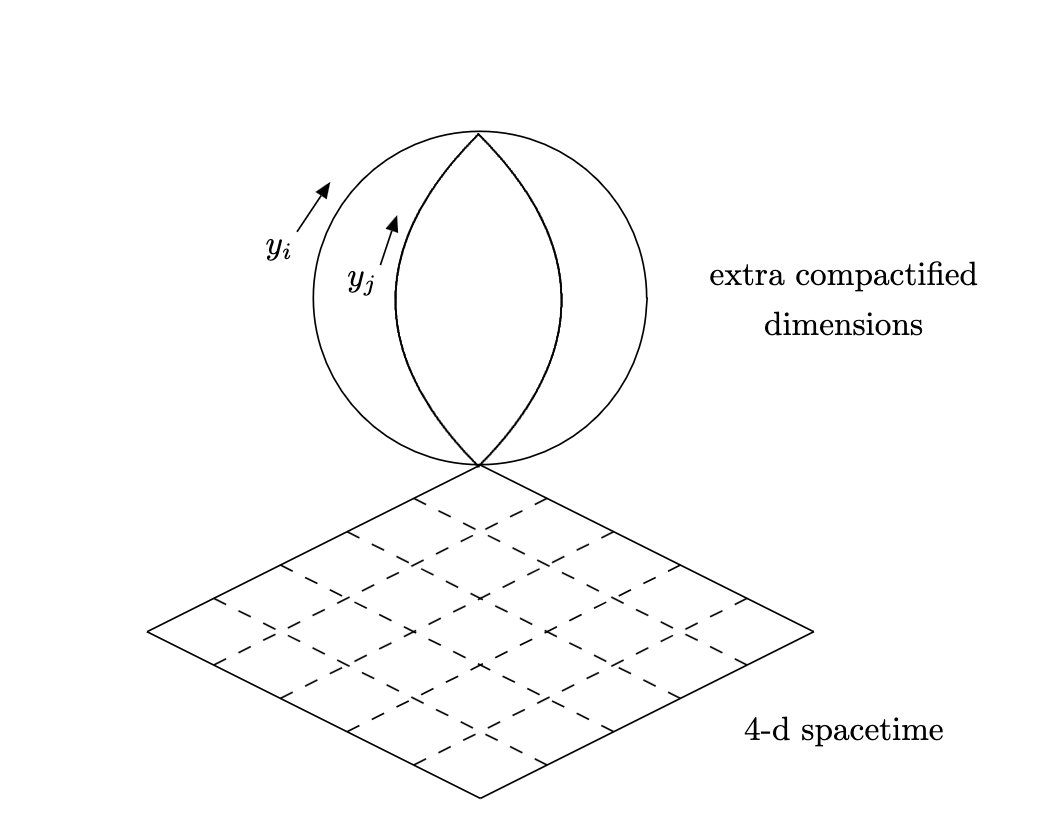
\includegraphics[scale=0.7]{fig/LEDsketch.png}
    \label{fig:LEDSketch}
\end{figure}

With this as a guiding principle, a new fundamental scale, much closer than the Planck scale and therefore experimentally accessible, is established. 
The Planck scale in terms of this new scale $M_D$ can be written as:

\begin{equation}
    \label{eq:NewPlanckMass}
    M^2_{Pl} = M_{D}^{2+n}R^n.
\end{equation}

To illustrate this, we follow the ideas given in the first paper on the ADD LED scenario~\cite{Arkani-Hamed:1998jmv}. Here, all SM particles and gauge interactions are confined our 4-dimensional brane which is embedded in a larger 4+$N$-dimensional bulk space, with $N$ extra dimensions that are compactified in a sphere or torus of radius R, with volume $V_n =(2 \pi R)^n$. In this 4+$N$ world, the gravitational potential between two masses $m_1$ and $m_2$, a distance $r \ll R$ from one another will feel a gravitational potential dictated by Gauss's law:

\begin{equation}
\label{eq:GaussLaw4D+nShort}
    V(r) \approx \frac{m_1m_2}{M^{N+2}_{Pl(4+N)}}\frac{1}{r^{n+1}}}, (r \ll R).
\end{equation}

If these two masses are separated with a distance $r \gg R$ from one another, their gravitational flux is too weak to penetrate the the extra dimensions so the usual $1/r$ potential is obtained,

\begin{equation}
\label{eq:GaussLaw4D+nLong}
    V(r) \approx \frac{m_1m_2}{M^{N+2}_{Pl(4+N)}R^N}\frac{1}{r}, (r\gg R).
\end{equation}

Comparing the two equations, we get the effective 4-D $M_{Pl}$, 

\begin{equation}
\label{eq:Mplanck_MEW}
   M^2_{Pl} \approx  M^{2+N}_{Pl(4+N)}R^N.
\end{equation}

This is equivalent to Eq.~\ref{eq:NewPlanckMass}.

For the hierarchy problem to be solved, we set $M_{D}\approx M_{EW}\approx1$~TeV, and demand that $R$ the observed $M_{Pl}$ yields,

\begin{equation}
    R \sim 10^{\frac{30}{n} -17} \text{cm}}\times\left(\frac{1~TeV}{m_{EW}}\right)^{1+\frac{2}{n}}.
\end{equation}

When $n=1$, the radius R is approximately $10^{13}$ centimeters which leads to observable deviations to Newtonian gravity within the solar system. This is clearly ruled out. For all cases $n \geq 2$, R goes at sub-mm distances. These are cases currently being explored in collider experiments and astrophysical and cosmological constraints are being set on the reduced Planck scale $M_D$ ~\cite{ParticleDataGroup:2020ssz}.

It's important to acknowledge that while the existence of large extra dimensions can address the hierarchy problem, it introduces another challenge in the form of a finely-tuned parameter: the size of the extra dimensions, R. As discussed earlier, R must be carefully chosen to match the 4D Planck scale and ensure that $M_D$ is on the Electroweak (EW) scale. This requirement replaces the need for fine-tuning of the bare Higgs boson mass. Regardless of our confidence in the ADD model specifically, it inspires a range of experiments to detect potential deviations from the Standard Model (SM). 

\subsubsection{ADD Phenomenology}

The Einstein-Hilbert Action for the ADD model can be 
pieces~\cite{Kribs:2006mq}: 

% The action of the ADD model can be decomposed into two pieces~\cite{Kribs:2006mq}: 

\begin{equation}
    \label{eq:ADDAction}
    S = S_{bulk} + S_{brane}
\end{equation}

where we are assuming that there is only one brane where the SM fields exist. The bulk action is just the Einstein-Hilbert Action for $4+n$ dimensional gravity:

\begin{equation}
    \label{eq:SBulkADD}
     S_{bulk} = -\int d^{(4+n)}x \sqrt{g^{4+n}}M^{n+2}_{D} \, R^{(4+n)}, 
\end{equation}

where $R^{(4+n)}$ is the higher-dimensional Ricci curvature scalar. 

In terms of the lagrangian density for the lagrangian density of the bulk fields $\phi(x,\Vec{y})$, we have:
\begin{equation}
    \label{eq:SBulkADD}
     S_{bulk} = \int d^{4}xd^ny \sqrt{|g^{4+n}|} \mathcal{L}(\phi(x,\Vec{y})), 
\end{equation}, 

Here $x$ stands for the (3+1) coordinates of the brane and $y$ is for the n extra dimensions ~\cite{Perez-Lorenzana:2005fzz}. On the other hand the action for the Brane Fields, $\xi(x)$ is written as
\begin{equation}
    \label{eq:SBraneADD}
     S_{Brane} = \int d^{4}xd^ny \sqrt{|g^{4+n}|} \mathcal{L}(\xi(x)) \delta^{n}(\Vec{y}-y_0), 
\end{equation}
where the use of the delta density promotes the fields to a higher dimensional expression. The brane is taken to be at a position $\Vec{y}=\Vec{y_0}$.

The line element in the bulk is 

\begin{equation}
    \label{eq:ADDBulkMetric}
    ds^2 = g^{4+n}_{\mu\nu}dx^{\mu}dx^{\nu}.
\end{equation}

The ADD model assumes spacetime is flat, in contrast to the RS model where it is warped. Hence, the metric tensor $g_{\mu\nu}$, the quantity that encodes the curvature of spacetime, can be expanded about flat spacetime with 4D metric fluctuations $h_{\mu\nu}$,

\begin{equation}
    \label{eq:ADDBulkMetric}
    ds^2 = (\eta_{\mu\nu} + h_{\mu\nu})dx^{\mu}dx^{\nu}-r^2d\Omega^2(n), 
\end{equation}

where $d\Omega_{(n)}$ are n-dimensional toroidal coordinates. Following the steps in ref.~\cite{Kribs:2006mq}, we can integrate out the higher dimensions and arrive at the result

\begin{equation}
    \label{eq:MplanckVolume}
    M^2_{\pl} = M^{n+2}_D (2 \pi r)^n,
\end{equation}

which is the same result in Eq.~\ref{eq:Mplanck_MEW} we quote in the previous section. The arbitrary metric fluctuations about the flat space time, $h_{\mu\nu}$ could be interpreted as the higher dimensional graviton which are laid out in more detail Refs.~\cite{Perez-Lorenzana:2005fzz,Kribs:2006mq, Giudice:1998ck}. Defining higher dimensional coordinates $y_i$, and imposing a periodic boundary conditions, $y_i \rightarrow y_i + 2\piR$ due to the compactifications of the extra dimensions, we have the expansion of the higher dimensional graviton in terms of the 4D Kaluza-Klein (KK) fields:

\begin{equation}
    \label{eq:KKexpansion}
    h_{\mu\nu} = \sum_{m1 = -\infty}^{\infty} ... \sum_{mn = -\infty}^{\infty} \frac{h^{(m)}_{\mu\nu}(x)}{\sqrt{V_n}} e^{i\frac{m_jy_j}{R}},
\end{equation} 

where $h^{m}$ is shorthand for $h^{(m_1,m_2,...m_n)}$. 
These KK graviton excitations or "tower" results from the coupling of the graviton to SM fields. Each of these KK modes couple to the stress-energy tensor of the SM field by the strength of gravity. The KK mass is given by $m^2_n = m^2 + \frac{k^2}{r^2}$. This mass spectrum, illustrated in Fig.~\ref{fig:KKmassSpectrum}, can be much less than the detector resolution. These discrete KK states are closely-spaced together and get closer together and appear as a continuum. In this CMS analysis, we look at the invariant diphoton mass spectrum illustrated by a result from a previous analysis in Fig.~\ref{fig:CMSModelDiphotonInvMass}~\cite{CMS:2011uvc}. The closely spaced KK modes are therefore predicted to appear as a continuum excess in the diphoton mass spectrum. 

\begin{figure}[!htbp]
    \centering
    \caption{Mass spectrum for KK gravitons for $n=2$.}
    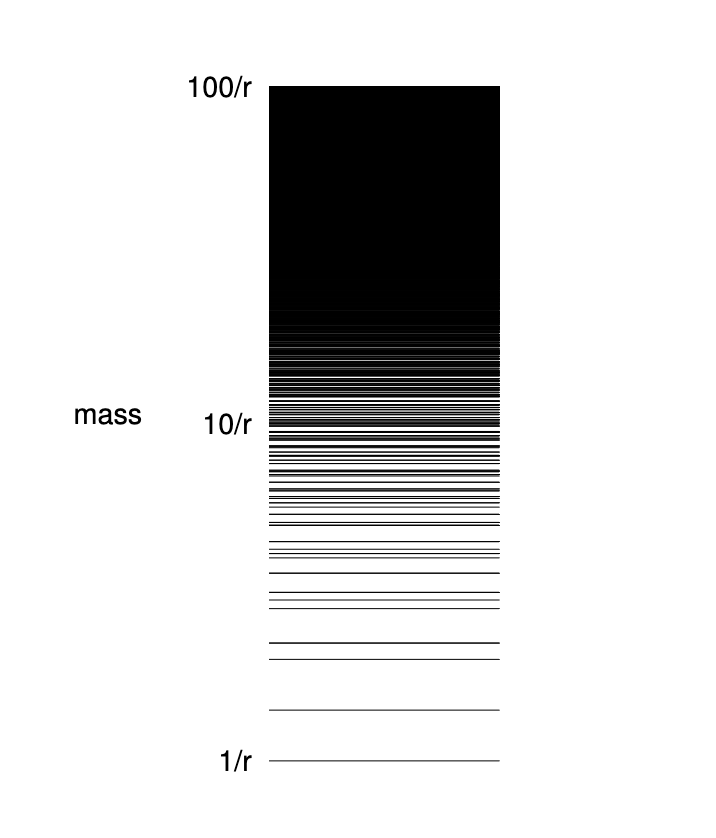
\includegraphics[scale=0.4]{fig/KKMassSpectrum.png}
    \label{fig:KKmassSpectrum}
\end{figure}


\begin{figure}[!htbp]
    \centering
     \caption{A CMS result~\cite{CMS:2011uvc} using data from $\sqrt{s} = 7$~\TeV pp-collisions which shows a comparison of the invariant mass spectrum predicted for the Standard Model diphoton production in light blue, overlayed with a continuous spectra for two Large Extra Dimensions signal points shown in dashed lines. The observed data and additional background predictions from $\gamma+$jet and dijet events are also shown in various markers indicated in the legend.}
    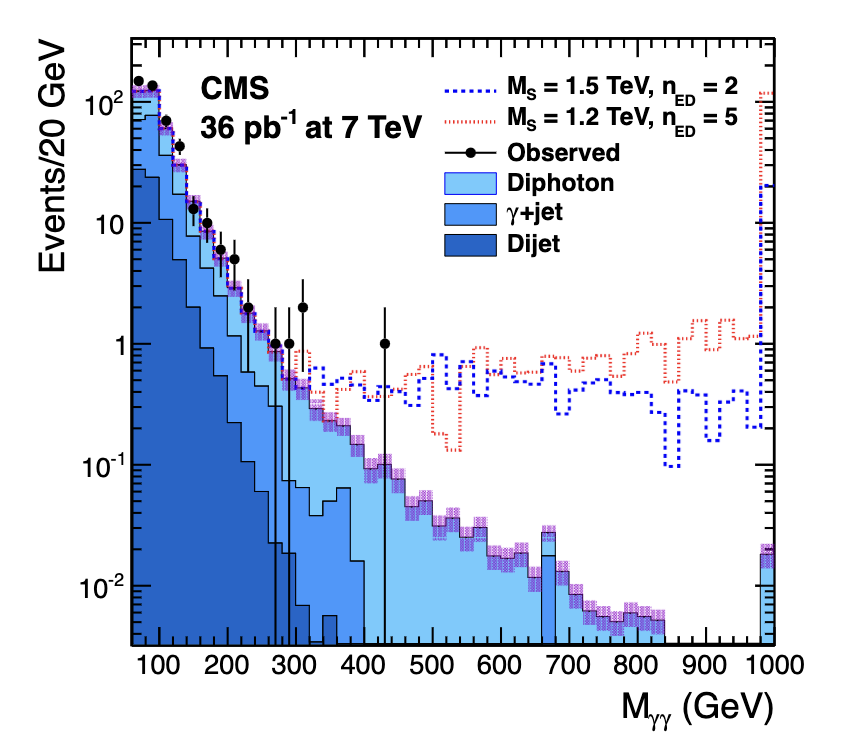
\includegraphics[scale=0.6]{fig/InvariantMass.png}
    \label{fig:CMSModelDiphotonInvMass}
\end{figure}


Since there are an infinite number of KK modes, an ultraviolet (UV) cutoff $M_s$ is introduced to get a non-diverging cross-section. The cross-sections for the virtual graviton exchange (see Fig.~\ref{fig:FeynmanDiagramUG}) for various parameters are shown in in Appendix~\ref{ch:appendix_signal_monte_carlo}. Any contributions above the cutoff scale $M_s$ is set to zero. The total cross-section is a combination of the contributions from the SM, ADD as well as the interference between the SM and ADD:

\begin{equation}
\sigma_{total} = \sigma_{SM} + \frac{\mathcal{F}}{M^4_{S}} \sigma_{int}+\frac{\mathcal{F}}{M^8_{S}} \sigma_{ADD} 
\label{eq:totalADDxsec}
\end{equation}

Here, $\mathcal{F}$ is parameter which allows us to translate our results in the different conventions for the ADD model that are found in literature. Here we  consider the GRW~\cite{Giudice:1998ck}, HLZ~\cite{Han:1998sg} and the Hewett~\cite{Hewett:1998sn} conventions where we have, 

\begin{equation}
\mathcal{F}=
    \begin{cases}
        1 & \text{if } \textnormal{GRW} \\
        log\left(\frac{M^2_s}{\hat{s}}\right) & \text{if } n_{ED} = 2 \\
        \frac{2}{n_{ED} - 2} & \text{if } n_{ED} > 2 \\
        \pm \frac{2}{\pi} & \text{if } \textnormal{Hewett}.
    \end{cases}
    \label{eq:KKConventions}
\end{equation} 

Here $\hat{s}$ is the centre-of-mass energy of the colliding partons. It is important to note that the GRW and the HLZ conventions interfere constructively while the Hewett could either interfere constructively (+) or destructively (-), according to the signs in Eq.~\ref{eq:KKConventions}. Later in Ch.~\ref{ch:SignalModelling}, $M_s$, is replaced by $\Lambda_{T}$ whose equivalence varies by convention.

% \begin{equation}
% \mathcal{F}=
%     \begin{cases}
%         1 & \text{if } x \in \mathbb{Q}\\
%         log\left(\frac{M^2_s}{\hat{s}}\right) & \text{if } x \in \mathbb{R}\setminus\mathbb{Q}
%     \end{cases}
% \end{equation}



\begin{figure}[!htbpt]
    \centering
     \caption{Feynman Diagrams for virtual graviton or Unparticle exchange in the diphoton channel $\gamma\gamma$ through quark annihilation (left) and gluon fusion (right).}
    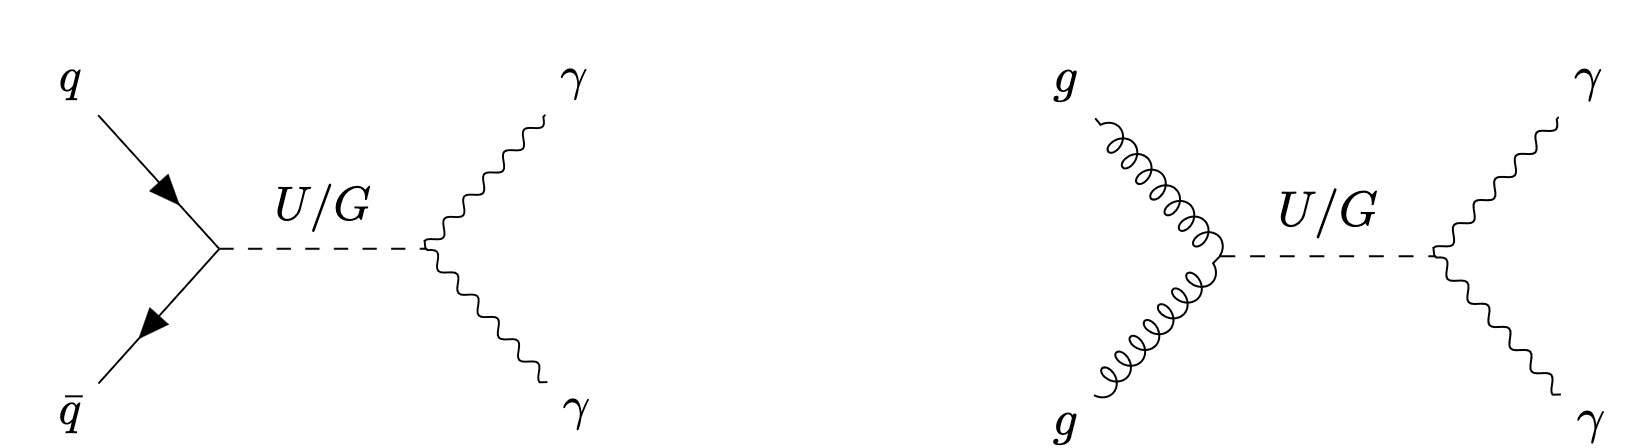
\includegraphics[scale=0.5]{fig/FeynmanDiagramUG.png}
    \label{fig:FeynmanDiagramUG}
\end{figure}

\subsection{Clockwork/ Linear Dilaton}~\label{sec:CWmodel} 
A more recent model that has been proposed is the Continuum Clockwork model which is equivalent to the Linear Dilaton theory in 5D. The CW/LD model is distinct but related to the more known extra-dimensional models which are the ADD LED and the RS Graviton scenarios. In the clockwork picture, the hierarchy is solved by introducing a continuum of clockwork fields which interact with each other. Inspired by gears transmitting energy, they are arranged in a way that the fields/particles associated have increasing masses/energy scales as you move along the chain as seen in Fig.~\ref{fig:ClockworkSchematic}.
This general mechanism can take large effective interaction scales from dynamics occuring at much lower energies. These ``gears" could also be interpreted as N copies of some particle content laid out on a one-dimensional lattice in theory space. In the continuum limit this lattice interpreted as a physical extra dimension and the gears are the KK modes~\cite{2Clockwork}. 

The basic mathematical setup of the CW/LD follows from Ref.~\cite{Giudice:2017fmj}. A 5D space is considered in which the extra dimension is a circle parametrized by $y$ where $- \pi R \leq y \leq \pi R$. The SM or TeV brane is set at $y = 0 $, whereas the Planck brane is set at $y = y_p = \pi R$. With a $Z_2$ orbifold symmetry, $y\leftrightarrow-y$ are identical. The full action in the Einstein frame is a sum of the SM action, the Bulk action and additional terms account for the extrinsic curvature of the two boundaries and the scalar potentials at the TeV and Planck branes near their local minima.

\begin{figure}[!htbp]
    \centering
    \caption{The ``Clockwork gears" schematic representation of the clockwork mechanism where the gears represent the interacting fields.~\cite{2Clockwork}. }
    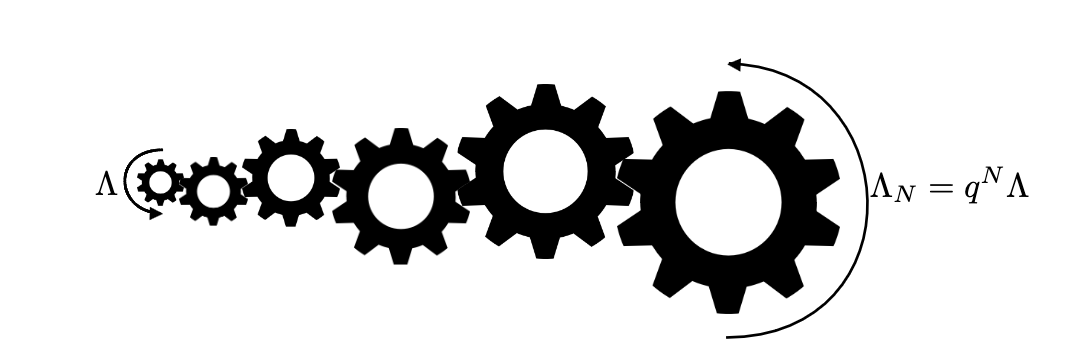
\includegraphics[scale=0.5]{fig/ClockworkSchematic.png}
    \label{fig:ClockworkSchematic}
\end{figure}

In this scenario, Einstein's equations and the dilaton equation of motion are solved by the metric,

\begin{equation}
    \label{eq:CWMetric}
    ds^2 = e^{\frac{4}{3}ky}g_{\mu\nu}dx^{\mu}dx^{\nu} + dy^2.
\end{equation}

Taking into account the metric in Eq.3.34 of Ref.~\cite{2Clockwork} which describes the graviton fluctuations around the 4D Minkowski space, we can write the decomposed graviton states as:

\begin{equation}
    \label{eq:GravitonEigenstates}
    h_{\mu\nu}=  \sum_{n = 0}^{\infty} \frac{\tilde{h}_{\mu\nu}(x) \Psi_n(y)}{\sqrt{\pi R}}.
\end{equation}

If we suppose that the SM fields localized at $y=0$, we can write the interaction lagrangian as 


\begin{equation}
    \label{eq:GravIntclockwork}
    \mathcal{L} = -\frac{h_{\mu\nu}(x,0)T^{SM}_{\mu\nu}(x)}{M^{3/2}_5} = -\sum_{n = 0}^{\infty} \frac{\tilde{h}_{\mu\nu}(x) T^{SM}_{\mu\nu}(x)}{\Lambda_n}, 
\end{equation}

where $T^{\textnormal{SM}}_{\mu\nu}(x)$, is the SM energy-momentum tensor and $\Lambda_n$ is the effective scale of interaction. In more detail these are written as, 

\begin{equation}
\label{eq:TuvAndIntScale}
T^{SM}_{\mu\nu}(x) &= -2\frac{\partial \mathcal{L}^{SM}}{\partial g_{\mu\nu}} + g_{\mu\nu}\mathcal{L}^{\textnormal{SM}} ; \quad
\Lambda_n &\equiv \frac{\sqrt{\pi R M^{3/2}_5}}{\psi_n(0)}.
\end{equation}

With this metric and the action, (see Appendix A of Ref.~\cite{2Clockwork}) one can derive the analogue to Eq.~\ref{eq:NewPlanckMass},

\begin{equation}
    \label{eq:MP_CW}
    M^2_{P} \approx \frac{M^3_5}{k} \left(e^{2 \pi kR-1}\right),
\end{equation}

where $M_5$ is the fundamental scale or the 5D reduced Planck Mass $M_D$.
This is the scale at which the theory must be UV-completed and it is assumed to be close to $M_{EW}$. Here, $M_P$ is an illusion caused by exponential factor, similar to the RS scenario. Using the Eq.~\ref{eq:TuvAndIntScale}, Eq.~\ref{eq:MP_CW}, as well as Eq.3.16 and 3.17 of Ref.~\cite{2Clockwork}, the effective scales of gravitational interaction are:
\begin{equation}
\label{eq:CWKInteractionScales}
\Lambda_0 &= M_P; \quad
\Lambda_n &= \sqrt{M^3_5 \pi R \left(1 + \frac{k^2 R^2}{n^2}  \right)}.
\end{equation}

To account for hierarchy, one needs to choose an appropriate $kR$ and expand the natural logarithm

\begin{equation}
    \label{eq:kRCW}
    kR \approx \frac{1}{\pi} ln\left(\frac{M_P}{M_5} \sqrt{\frac{k}{M_5}}\right) \approx 10 + \frac{1}{2\pi}ln\left(\frac{k}{\textnormal{TeV}}\right)-\frac{3}{2\pi}ln\left(\frac{M_5}{10\textnormal{TeV}}\right).
\end{equation}

Here, $k$ is a mass parameter called the ``clockwork spring" which measures the effectiveness of the clockwork mechanism. A flat metric corresponds to $k = 0$. As described in the original paper, the extra dimension is discretized by choosing $y_j = ja$, where $j = 0,...,N$. The lattice spacing $a$ is such that $Na = \pi R$. While this construction resembles fields in a deconstructed flat extra dimension, there is a critical difference which comes from how each link breaks the symmetry of a single gear site. A parameter q treats the site $j+1$ and the site $j$ (with $j = 0,..., N - 1$) asymmetrically. It's important to note that we can establish a total of $N$ connections among the $N + 1$ available sites. As a consequence, one site retains its masslessness. For q to remain $y$-independent and for $q^N$ to give a finite but non-trivial clockwork behavior, as the number of sites approaches infinity, we set 

\begin{equation}
    \label{eq:qEq}
    q^N = e^{k \pi R}.
\end{equation}

The excitations have a similar form with the large extra dimensions, where at the large N limit, we have

\begin{equation}
\label{eq:CWKKModes}
m^2_0 &= 0; \quad
m^2_n &= k^2 + \frac{n^2}{R^2} + \frac{O(1)}{N}, \quad n = 1, \ldots, N
\end{equation}

which appears as a continuous spectrum like the ADD LED but with evenly distributed energy levels and mass-squared splitting equal to the inverse radius-squared. However, we will see later in Ch.~\ref{ch:SignalModelling} that the spectrum shifts by an amount equal to the clockwork spring constant k, introducing a mass gap~\cite{2Clockwork}. 

\subsection{Unparticles Model}~\label{sec:UnparticlesModel}
The two previous models propose scenarios which address the hierarchy problem via the existence of extra spatial dimensions. The Unparticles~\cite{Georgi_2007unpar} model on the other hand, addresses the hierarchy problem by introducing a new energy scale related to a yet-to-be-seen scale-invariant Banks-Zaks ($\mathcal{BZ}$) sector where ``unparticle stuff" live. If this sector exists, there are measureable effects coming from the interactions between the Standard model particles and the these hidden sector Unparticles. This has particular consequences with the Higgs naturalness problem - a dilemma where the Higgs mass receives quantum corrections that are quadratically sensitive to the energy scale of new Physics. Instead of the scale being at $M_P$, this new scale could be much closer via the existence of the $\mathcal{BZ}$ and the unparticle-SM interactions could help redistribute the quantum corrections and potentially reduce the fine-tuning problem~\cite{Kikuchi:2007qd}.

While not directly related to this dissertation, the Unparticles model can also potentially address issues related to flavor physics and CP violation via new interactions through the hidden sector and modifications in the flavor-changing and CP-violating processes that could still be consistent with experimental observations~\cite{Georgi_2007unpar, Chen:2007vv,Freitas:2007ip, Zwicky:2007vv}.

In the first paper by Georgi~\cite{Georgi_2007unpar}, the scale-invariant $\mathcal{BZ}$ sector must interact weakly with the Standard Model. Such a sector could not have particles of definite non-zero mass as mass terms explicitly breaks scale invariance.
It only holds ``Unparticles" which is a hazy concept that is different from our familiar notion of particulate notion of particulate matter. However, using a low-energy ``Effective field theory" (EFT), some phenomenological exploration is possible. 

% Thus the domain of utility of an effective theory is necessarily bounded
% from above in energy scale

In general, direct searches are only possible if the form of the BSM theory is established, but an EFT~\cite{Georgi:1993mps} approach allows us to quantify deviations from SM predictions of known particles without introducing additional assumptions about the BSM theory. The only assumption made is that the BSM theory will faithfully reproduce the SM in the regime where it is already empirically validated. As mentioned earlier, we can surmise that the SM is an effective field theory of some higher-energy theory which is valid to some cut-off energy scale $\Lambda$. 

For the Unparticles scheme, the new higher energy theory contains the SM fields and the $\mathcal{BZ}$ fields, which has a nontrivial IR fixed point. The two sets of fields interact via the exchange of particles with a large Mass Scale $M_{\mathcal{U}}$. Below this scale the interaction can be described by non-renormalizable couplings suppressed by powers of  $M_{\mathcal{U}}$ and we can write the interacting lagrangian in the following form

\begin{equation}
    \label{eq:LagIntUnpar}
    \mathcal{L}_{int} = \frac{1}{M^k_{\mathcal{U}}} \mathcal{O}_{SM}\mathcal{O}_{\mathcal{BZ}}
\end{equation}

where $\mathcal{O}_{SM}$  is an operator with mass dimension $d_{SM}$ that is built out of SM fields and $\mathcal{O}_{\mathcal{BZ}}$ is an operator $d_{\mathcal{BZ}}$ built out of $\mathcal{BZ}$ fields. The exponent $k= d_{SM} + d_{BZ}-4$.

At energy $\Lambda_{\mathcal{U}}$, the $\mathcal{BZ}$ sector emerges and it is expected to be conformal. However, this coupling transmutes as the energy increases to $\Lambda_{\mathcal{U}}$ as the scale invariance or conformal invariance is expected. In the effective theory below  $\Lambda_{\mathcal{U}}$, the $\mathcal{O}_{\mathcal{BZ}}$ operators match unto Unparticle operators and the interactions match onto the following form

\begin{equation}
    \label{eq:LagIntUnparMatch}
    \mathcal{L}_{int} =  \frac{C_{\mathcal{U}}\Lambda^{d_{BZ}-d_{SM}}_{\mathcal{U}}}{M^k_{\mathcal{U}}}\mathcal{O}_{SM}\mathcal{O}_{\mathcal{U}} = 
    \frac{\lambda}{ 
    \Lambda_{\mathcal{U}}^{ d_{\mathcal{U}}+d_{SM}-4}}} }\mathcal{O}_{\mathcal{U}}\mathcal{O}_{SM}
\end{equation}

Here $\mathcal{O}_{\mathcal{U}}$ is the Unparticle operator with dimension $d_{\mathcal{U}}$, $\lambda$ is the coupling constant between SM and $\mathcal{BZ}$. Georgi observed that the Unparticle mass spectrum looked like a $d_{\mathcal{U}}$ number of invisible massless particles. Following the arguments from Ref.~\cite{Georgi_2007unpar, Cheung:2007ap, CheungEtAl:2007}, scale invariance can be used to fix the two-point functions of these unparticle operators to show this effect. Consider a the vacuum matrix element, $\mathcal{O}_{\mathcal{U}}$,

\begin{equation}
\begin{align*}
    \langle 0|\mathcal{O}_{U}(x)\mathcal{O}_{U}^\dagger (0)|0\rangle 
    &= \langle 0|e^{i\hat{P}\cdot x}O_U(0)e^{-i\hat{P}\cdot x}O_U^\dagger (0)|0\rangle \\
    &= \int d\lambda \int d\lambda' \langle0| \mathcal{O}_{U}(0)|\lambda'\rangle 
    \times \langle \lambda'| e^{i\hat{P}\cdot x} |\lambda\rangle 
    \langle \lambda| \mathcal{O}^\dagger_{U}(0) |0\rangle \\
    &= \int \frac{d^{4}P}{(2\pi)^4} e^{i\hat{P}\cdot x} \rho_{\mathcal{U}} (P^2),
\end{align*}
\label{eq:TwoPointFuncUnpar}
\end{equation}

where $\rho_{\mathcal{U}} (P^2)$ is a spectral density given by:

\begin{equation}
\rho_{\mathcal{U}} (P^2) = A_{d_{\mathcal{U}}} \theta(P^0)\theta(P^2)(P^2)^{d_{\mathcal{U}}-2}.
\end{equation}

Here $P$ is the invariant Unparticle mass $P$, $\theta$ is the Heaviside step function, and $ A_{d_{\mathcal{U}}} $ is the normalization factor. The heaviside step functions $\theta(P^0)$, $\theta(P^2)$ ensure that the only positive energy solutions and that the unparticle stuff is not tachyonic, respectively~\cite{Kenzie:2022nza}. As shown in ref.~\cite{Cheung:2007ap}, under scale transformations $x \rightarrow sx $ and 
$\mathcal{O}_{\mathcal{U}}(sx) \rightarrow s^{-d_{\mathcal{U}}}\mathcal{O}_{\mathcal{U}}(x)$, $ A_{d_{\mathcal{U}}} $ becomes

\begin{equation}
 A_{d_{\mathcal{U}}}= \frac{16\pi^2\sqrt{\pi}}{(2\pi)^{2d_{\mathcal{U}}}} \frac{\Gamma\left(d_{\mathcal{U}} + \frac{1}{2}\right)}{\Gamma\left(d_{\mathcal{U}} -1\right) \Gamma\left(2d_{\mathcal{U}}\right)}.
\end{equation}

This phase space is the same as that for $d_{\mathcal{U}}$ massless particles, where $d_{\mathcal{U}}$, can be a fractional number. 

\subsubsection{Unparticle Physics to Diphotons}

There are several papers~\cite{Kumar:2007af, Kumar:2008dn, Ask:2009pv} in literature that explore the phenomenology of the Unparticle model decaying into two photons. In this dissertation, we consider scalar (Spin-0) and tensor (Spin-2) Unparticles. The virtual exchange of Unparticles, shown in Fig.~\ref{fig:FeynmanDiagramUG}, have the following associated matrix elements. For Spin-0, we have,


\begin{align*}
     |\bar{M}_{q\bar{q}}|^2 &= \frac{1}{8N_c} \lambda^4 \chi^2_{\mathcal{U}} \left(\frac{s}{\Lambda^2_{\mathcal{U}}}\right)^{2d_{\mathcal{U}}-1}, \\
     |\bar{M}_{gg}|^2 &= \frac{1}{8\left(N^2_c-1\right)}\frac{1}{4} \lambda^4 \chi^2_{\mathcal{U}} \left(\frac{s}{\Lambda^2_{\mathcal{U}}}\right)^{2d_{\mathcal{U}}}.
\end{align*}
~\label{eq:Unparspin0Matrix}

And for Spin-2 Unparticles, 
\begin{align*}
|M_{q\bar{q}}|^2 &= \frac{1}{8N_c} \left[ e^4Q_f^4 8 \left( \frac{u}{t} + \frac{t}{u}\right) \right] \\
&\quad - 8e^2Q_f^2\lambda^2_t\chi_{U} \cos(d_{U}\pi) \left(\frac{s}{\Lambda^2_{U}}\right)^{d_U} \frac{1}{s^2} \left(u^2 + t^2\right) \\
&\quad + 2 \lambda^4_t \chi^2_{U} \left(\frac{s}{\Lambda^2_{\mathcal{U}}}\right)^{2d_{\mathcal{U}}} \frac{1}{s^4} \left(u^4+t^4\right), \\
|\bar{M}_{gg}|^2 &= \frac{1}{8(N^2_c-1)}2 \lambda^4_t \left(\frac{s}{\Lambda^2_{\mathcal{U}}}\right)^{2d_{\mathcal{U}}}\chi^2_{U} \frac{1}{s^4} \left(u^4+t^4\right)
\end{align*}
~\label{eq:Unparspin2Matrix}
where $Q_f$ is the electric charge of the parton with flavor $f$,$\chi_{U} = \frac{A_{d_{\mathcal{U}}}}{2\sin(d_{\mathcal{U}} \pi)}$ and $N_c$ is the number of colors. The variables $s, t, u$ are the Mandelstam variables. It can be seen in the above equations that only Spin-2 tensor Unparticles interfere with the SM subprocess amplitudes. As the authors of ref.~\cite{Kumar:2007af} argued, that only $1< d_{u} <2$ is the viable range that could be explored in the LHC. It is also important to note that due to the factor $\Lambda^{-d_{U}}_U$ in Eqs.~\ref{eq:Unparspin0Matrix} and ~\ref{eq:Unparspin2Matrix}, the cross sections are suppressed with increasing $\Lambda_{U}$. The cross section also scales with the Wilson coefficient, $\frac{\lambda}{\Lambda_{u}}$.
 
\subsubsection{Unparticles and Extra Dimensions}

The Unparticles model and Extra Dimensions have been shown to have similar collider signatures. The calculation of their cross-sections are similar as they share analogous phase-space integrations~\cite{Ask:2009pv, Cheung:2007ap}. In a simple case where a scalar field is identified as a massless scalar bulk field permeating into the LED. With this setup, the dimension of the Unparticle field $d_{\mathcal{U}}$ is related to the number of extra dimension~\cite{Cheung:2007ap} as follows
\begin{equation}
    d_{\mathcal{U}} = \frac{n}{2} +1
\end{equation}

In this context, incorporating the Unparticles model interpretation into the Search for Non-resonant Signal Models appears to hold promise as a scientifically valuable endeavour.

\subsection{Previous Searches}

The search for signatures of Large extra dimensions, CW/LD and Unparticles go beyond collider searches. However, we limit the discussion of previous results to collider searches here. The methods and results in this study has a direct precedent from the work published in Ref.~\cite{CMS:2018dqv}. Limits have been placed on the relevant model parameters for the ADD Large Extra Dimensions as shown on Table~\ref{tab:ADD_limits2016}, and the Clockwork model using high-mass diphoton events from the 2016 data from the CMS experiment (see Fig.~\ref{fig:ClockworkCMS2016}) which was at the time the most stringent limits on the ADD Large Extra Dimensions and the Clockwork Model. The total asymmetric uncertainties are shown on the expected limits for Table~\ref{tab:ADD_limits2016}. In Figure~\ref{fig:ClockworkCMS2016}, the shaded green and yellow bands represent the 1 and 2 standard deviation uncertainty in the expected limit. The theory becomes nonperturbative in the $k > M_5$ region denoted by the light purple shaded region. The region below and to the left of the solid line constitutes the excluded region. A complementary search has also been done on dilepton events~\cite{CMS:2021ctt}. Both searches showed no significant deviation from the SM expectation of unity.

\begin{table}[pt]
	\centering
	\caption{Previous exclusion limits results on the mass scale \Ms in {\TeVns} for various conventions used in the calculation of the ADD large extra-dimensional scenario using the 2016 CMS detector data corresponding to an integrated luminosity of 35.9 \fbinv~\cite{CMS:2018dqv} only. }
	\cmsTable{
	\begin{tabular}{cccccccccc}
		\\	
		\hline \hline
		\vspace*{-3.5mm} &&&&&&&&& \\
		\multirow{2}{*}{Signal} & GRW & \multicolumn{2}{c}{Hewett} & \multicolumn{5}{c}{HLZ} \\
		& & negative & positive & $\nED=2$ & $\nED=3$ & $\nED=4$ & $\nED=5$ & $\nED=6$ & $\nED=7$ \\ [\cmsTabSkip]
		\hline
		\vspace*{-2.5mm} &&&&&&&&& \\
		Expected & $7.1^{+0.7}_{-0.5}$ & $5.5^{+0.1}_{-0.3}$ & $6.3^{+0.6}_{-0.4}$ & $8.4^{+1.3}_{-1.1}$ & $8.4^{+0.8}_{-0.6}$ & $7.1^{+0.7}_{-0.5}$ & $6.4^{+0.6}_{-0.5}$ & $6.0^{+0.6}_{-0.4}$ & $5.6^{+0.6}_{-0.4}$ \\ [\cmsTabSkip]
		Observed & 7.8 & 5.6 & 7.0 & 9.7 & 9.3 & 7.8 & 7.0 & 6.6 & 6.2 \vspace*{1.0mm} \\
		\hline \hline
	\end{tabular}
	}
	\label{tab:ADD_limits2016}
\end{table}


\begin{figure}[!htbp]
    \centering
    \caption{2016 95\%  CL exclusion limits results for the continuous clockwork mechanism over the $k -M_5$ parameter space.}
    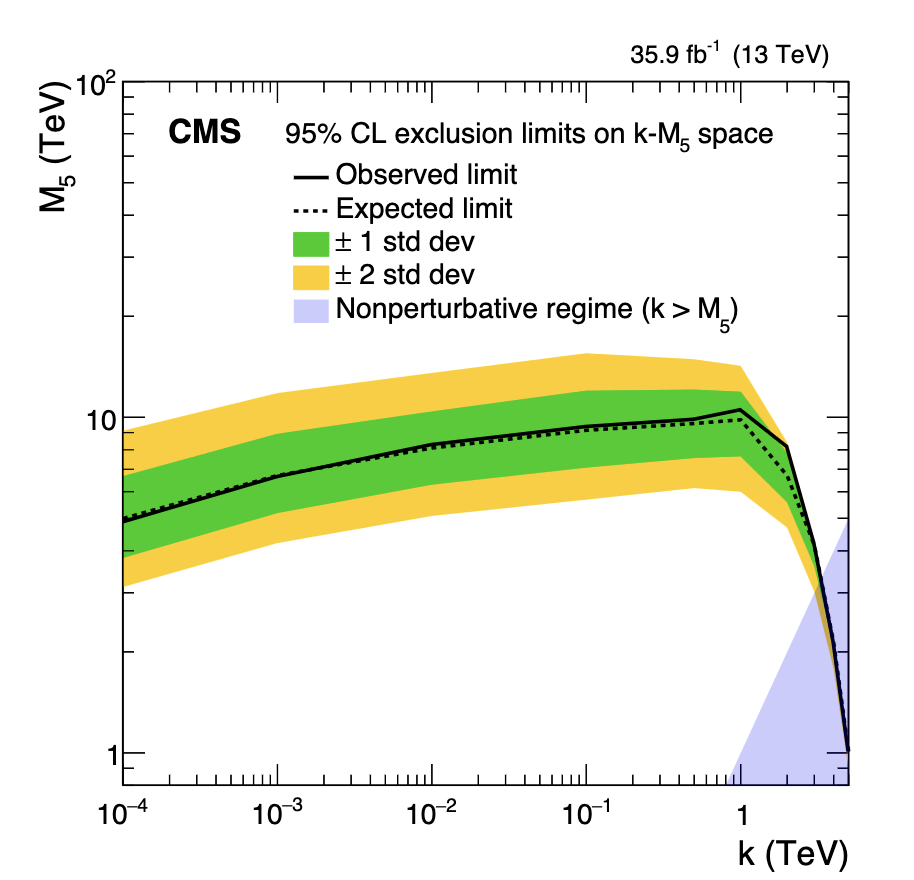
\includegraphics[scale=0.5]{fig/ClockworkCMS.png}
    \label{fig:ClockworkCMS2016}
\end{figure}


More recently, the ATLAS experiment~\cite{ATLAS:2023hbp} recently placed exclusion limits at 95\% on the two-dimensional parameter space of the clockwork gravity model in their search for periodic signals in the dielectron and diphoton mass spectrum. We compare these recent results with our latest findings in Ch.~\ref{ch:results}.

% \begin{figure}[ht]
%     \centering
%     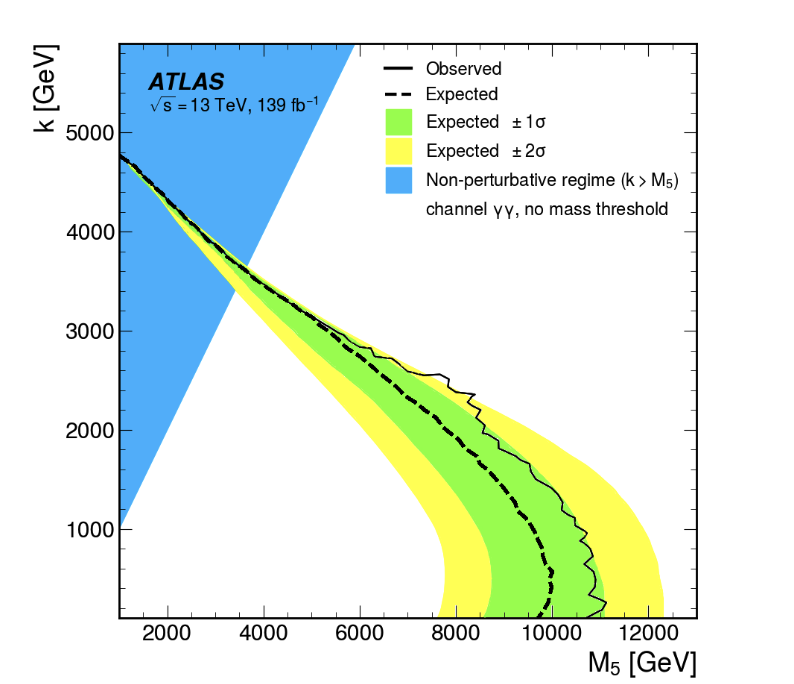
\includegraphics[scale=0.]{fig/ATLASkM5nomass.png}
%     \caption{The expected and observed exclusion limits at 95\% CL for the clockwork gravity model projected in the $k–M_5$ parameter space for the $\gamma\gamma$ channel for the case without mass thresholds. The shaded area with illustrates
% the region of phase space where the CW/LD theory becomes non-perturbative}
%     \label{fig:ATLASLimitsCW}
% \end{figure}

Both the Unparticles and Large Extra dimensions have also been used as additional model interpretations of Searches for Dark Matter that are produced in association with Z boson plus missing $E_{T}$ decays using the full Run II CMS data~\cite{CMS:2020ulv}. Figure~\ref{fig:UnparZMET} shows limits applied to fixed values of the effective cutoff scale $\Lambda_U$ = 15 TeV and the coupling constant $\lambda$ = 1. While this analysis involves a direct production rather than a virtual exchange of Unparticles, which is what is investigated here. The diphoton channel provides a complementary search where there is potentially more sensitivity for some values of $d_{\mathcal{U}}$ and $\Lambda_{\mathcal{U}}$.

\begin{figure}[!htbp]
    \centering
    \caption{A related report on the 95\% CL upper limits on unparticle+Z~\cite{CMS:2020ulv} production cross section, as a function of the scaling dimension $d_U$.}
    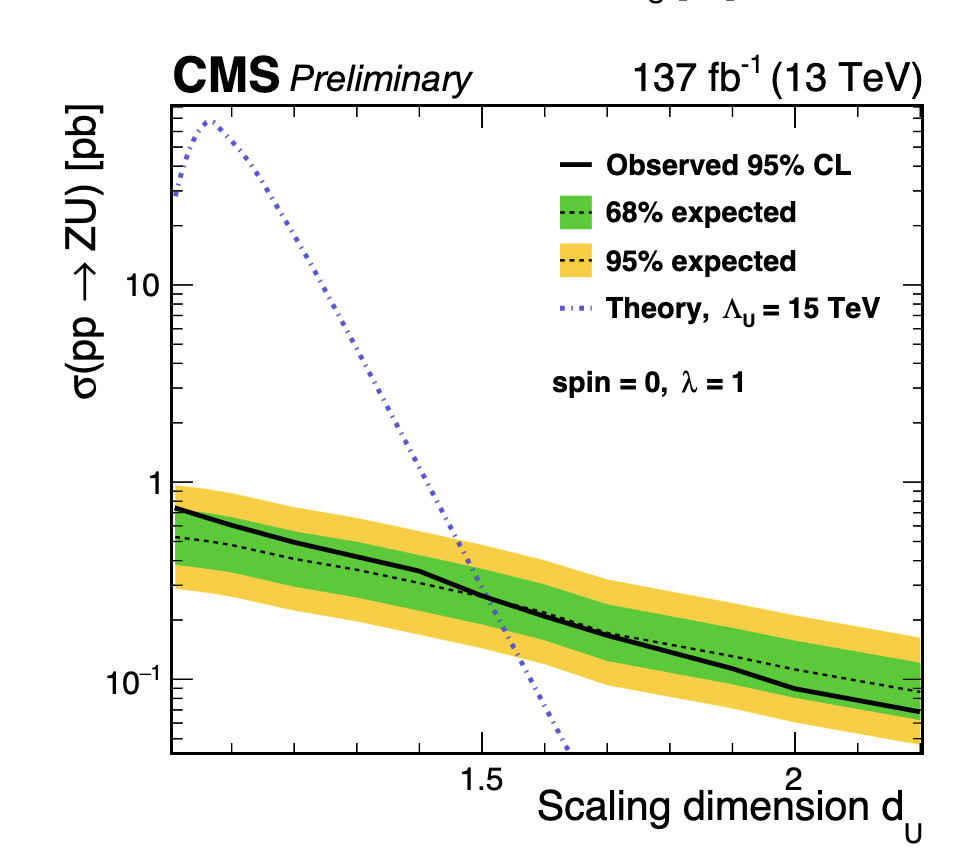
\includegraphics[scale=0.7]{fig/Unparticles.png}  
    \label{fig:UnparZMET}
\end{figure}

\newpage


% \renewcommand{\bibsection}{\topskip=32pt\chapter*{References}\topskip=0pt \addcontentsline{toc}{chapter}{References}\vspace*{6pt}}

% \begin{singlespacing}
% \bibliographystyle{lucas_unsrt.bst}
% \bibliography{references}
% \end{singlespacing}



\hypersetup{pageanchor=true}
\chapter{Experimental Setup: The Large Hadron Collider and the CMS Detector}~\label{ch:CMSExperiment}

{\small \rightline{“It doesn't matter how beautiful your theory is, it doesn't matter }
\vspace{-2ex}
\rightline{how smart you are. If it doesn't agree with experiment, it's wrong.”}
\rightline{-Richard Feynman}}
\vspace{4ex}

In this chapter, we discuss the experimental setup. First, in Sec~\ref{sec:LHC} we discuss the accelerator complex that accelerates protons into counter-rotating beams which are then collided to produce the two-photon events which are collected by the CMS detector~\ref{sec:CMSDetector}. 

\section{The Large Hadron Collider}~\label{sec:LHC}
\begin{figure}[!htb]
	\centering
	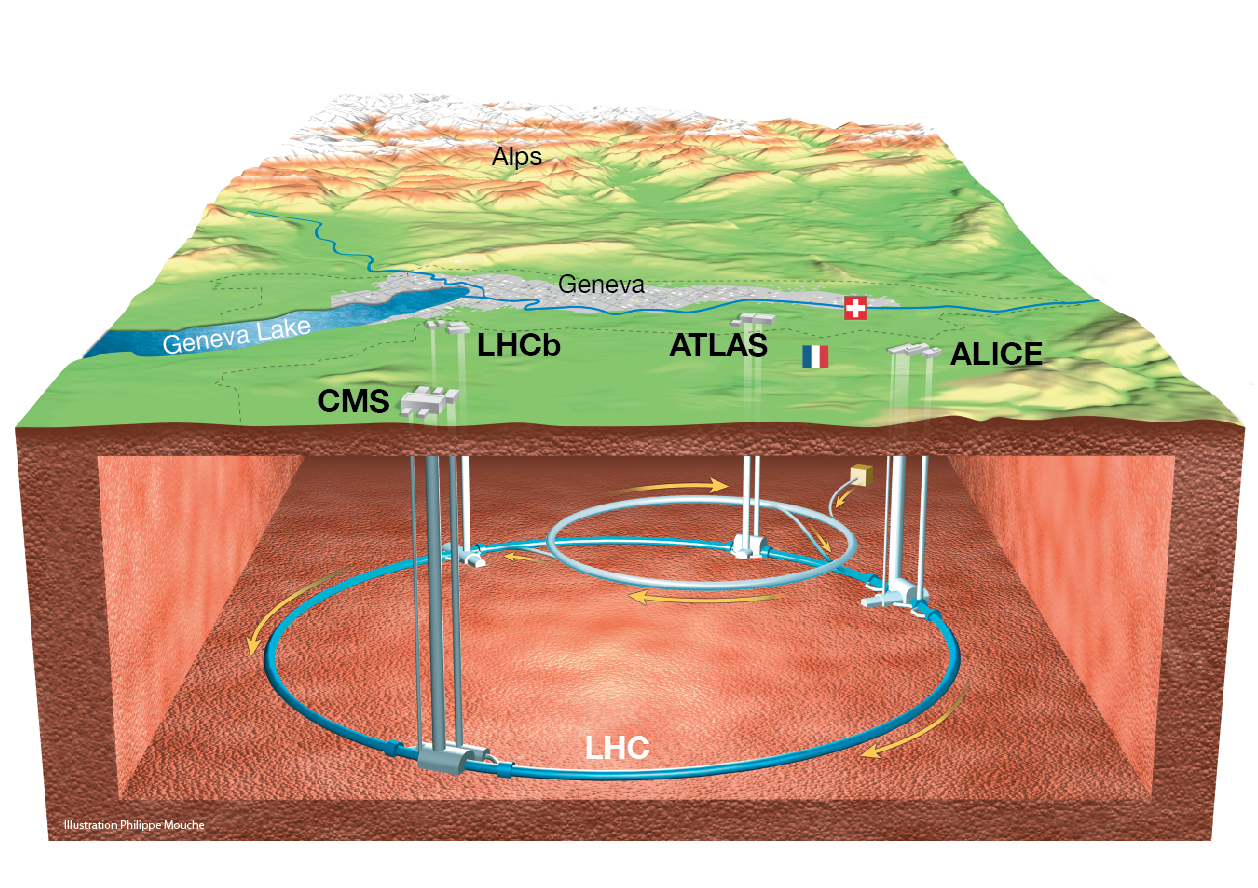
\includegraphics[scale=0.3]{fig/lhc_overview.png}
	\caption{A bird's eyeview and and schematic depiction of the underground LHC accelerator complex and its four interaction points in Geneva, Switzerland and France~\cite{Mouche:1708847}.}
	\label{lhc-overview}
\end{figure}


% \RaggedRight \parindent=25pt
\justifying \parindent=25pt


The Large Hadron Collider (LHC) depicted in Figure~\ref{lhc-overview}, is the world's largest and most powerful man-made particle accelerator as of date. It is nestled approximately 100 meters underground, beneath the Jura Mountains and Lac Leman, straddling Geneva, Switzerland and the neighbouring territory of France.

The LHC was built as a general purpose collider and the data it produces serve various physics programs from precision measurements in the Standard Model to searches for exotic, beyond standard model physics. In this section, we will briefly describe the LHC accelerator complex, the engineering motivations for the collider design and the key physics performance in various runs.

\subsubsection{LHC Ring of Magnets}
The full 27-km LHC ring is made up of segments of cryogenically-cooled superconducting dipole and quadrupole magnets that house two counter-rotating proton beam pipes. The dipole magnets steer the particle beams into an approximately circular orbit. Superconducting quadrupole magnets focus the particle beams while higher order moment magnets are used for beam corrections, all in the effort to maximize collision rates~\cite{Rossi:2002ye}. A total of 1248 dipole and 400 quadrupole magnets constitute the full ring, each of them 15-m and 3-m in length respectively. They are constructed with niobium-titanium (NbTi) which produce an operational field strength of 7.7 T. To maintain their superconductive state, they are cooled to 1.9 K with liquid helium.

\subsubsection{Experiments Overview}
 
 Protons are sourced from a bottle of hydrogen and end their journey when they collide at four interaction points in the LHC (see Figure~\ref{fig:accelerator_complex}). Around these interaction points are the four main experiments: ATLAS \cite{ATLAS:2008xda}, CMS \cite{CMS:2008xjf}, LHCb \cite{LHCb:2008vvz}, and ALICE \cite{ALICE:2008ngc}. ATLAS (A Toroidal LHC Apparatus) and CMS (Compact Muon Solenoid) are two of the general-purpose detectors that have similar physics programs where their results are often benchmarked against each other's. ALICE (A Large Ion Collider Experiment), focuses on heavy ion collisions and primarily studies the quark-gluon plasma. LHCb specializes on studying CP violation, or the investigating slight differences in matter and antimatter using ``beauty" quark decays. Four additional, auxiliary experiments also operate through these points, TOTEM, LHCf, MoEDAL and FASER.  

\subsubsection{The CERN Accelerator Complex}

Before the protons or lead ions reach the collision points, they first have to go through a series of accelerators shown in Figure~\ref{fig:accelerator_complex} to reach the desired total collision energy of 13 TeV for Run II. For the sake of brevity, we will only consider proton beams at this point but lead ions follow the same route but start from vaporized led. Protons, on the other hand, are sourced from molecular hydrogen which are ionized. Ionized hydrogen (H-) are then extracted and injected to Linac4 where Radiofrequency (RF) cavitites are used to accelerate them to 160 MeV. They are then prepared to enter the first of the circular accelerators called the Proton Synchrotron Booster (PSB). Before they enter the PSB, the ions are stripped of their electrons and the protons are accelerated to 2~\GeV. This prepares them for injection to the Proton Synchrotron (PS) which increases the beam energy to 26~\GeV. The final step prior to injection to the final LHC ring is in the Super Proton Synchrotron (SPS) where the beams reach up to 450~\GeV.
The proton beams take around 20 minutes to reach their maximum energy of 6.5~\TeV in the LHC ring and they can circulate for many hours inside the LHC beam pipes during normal operations. During collisions, the counter-rotating beams meat at the interaction points inside the four primary detectors described earlier.
% This means that the counter-rotating particle beams each have an energy of E = 6.5 TeV \cite{LHCpop}

% Once the proton beams are transferred into the two counter-rotating beam pipes of the LHC, it takes around 20 minutes for the protons to reach their maximum energy of 6.5 TeV. The beams can circulate for many hours inside the LHC beam pipes under normal operating conditions and during collisions, they meet at at the interaction points inside the four detectors described earlier. 


% \begin{figure}[!htbp]
% 	\centering
% 	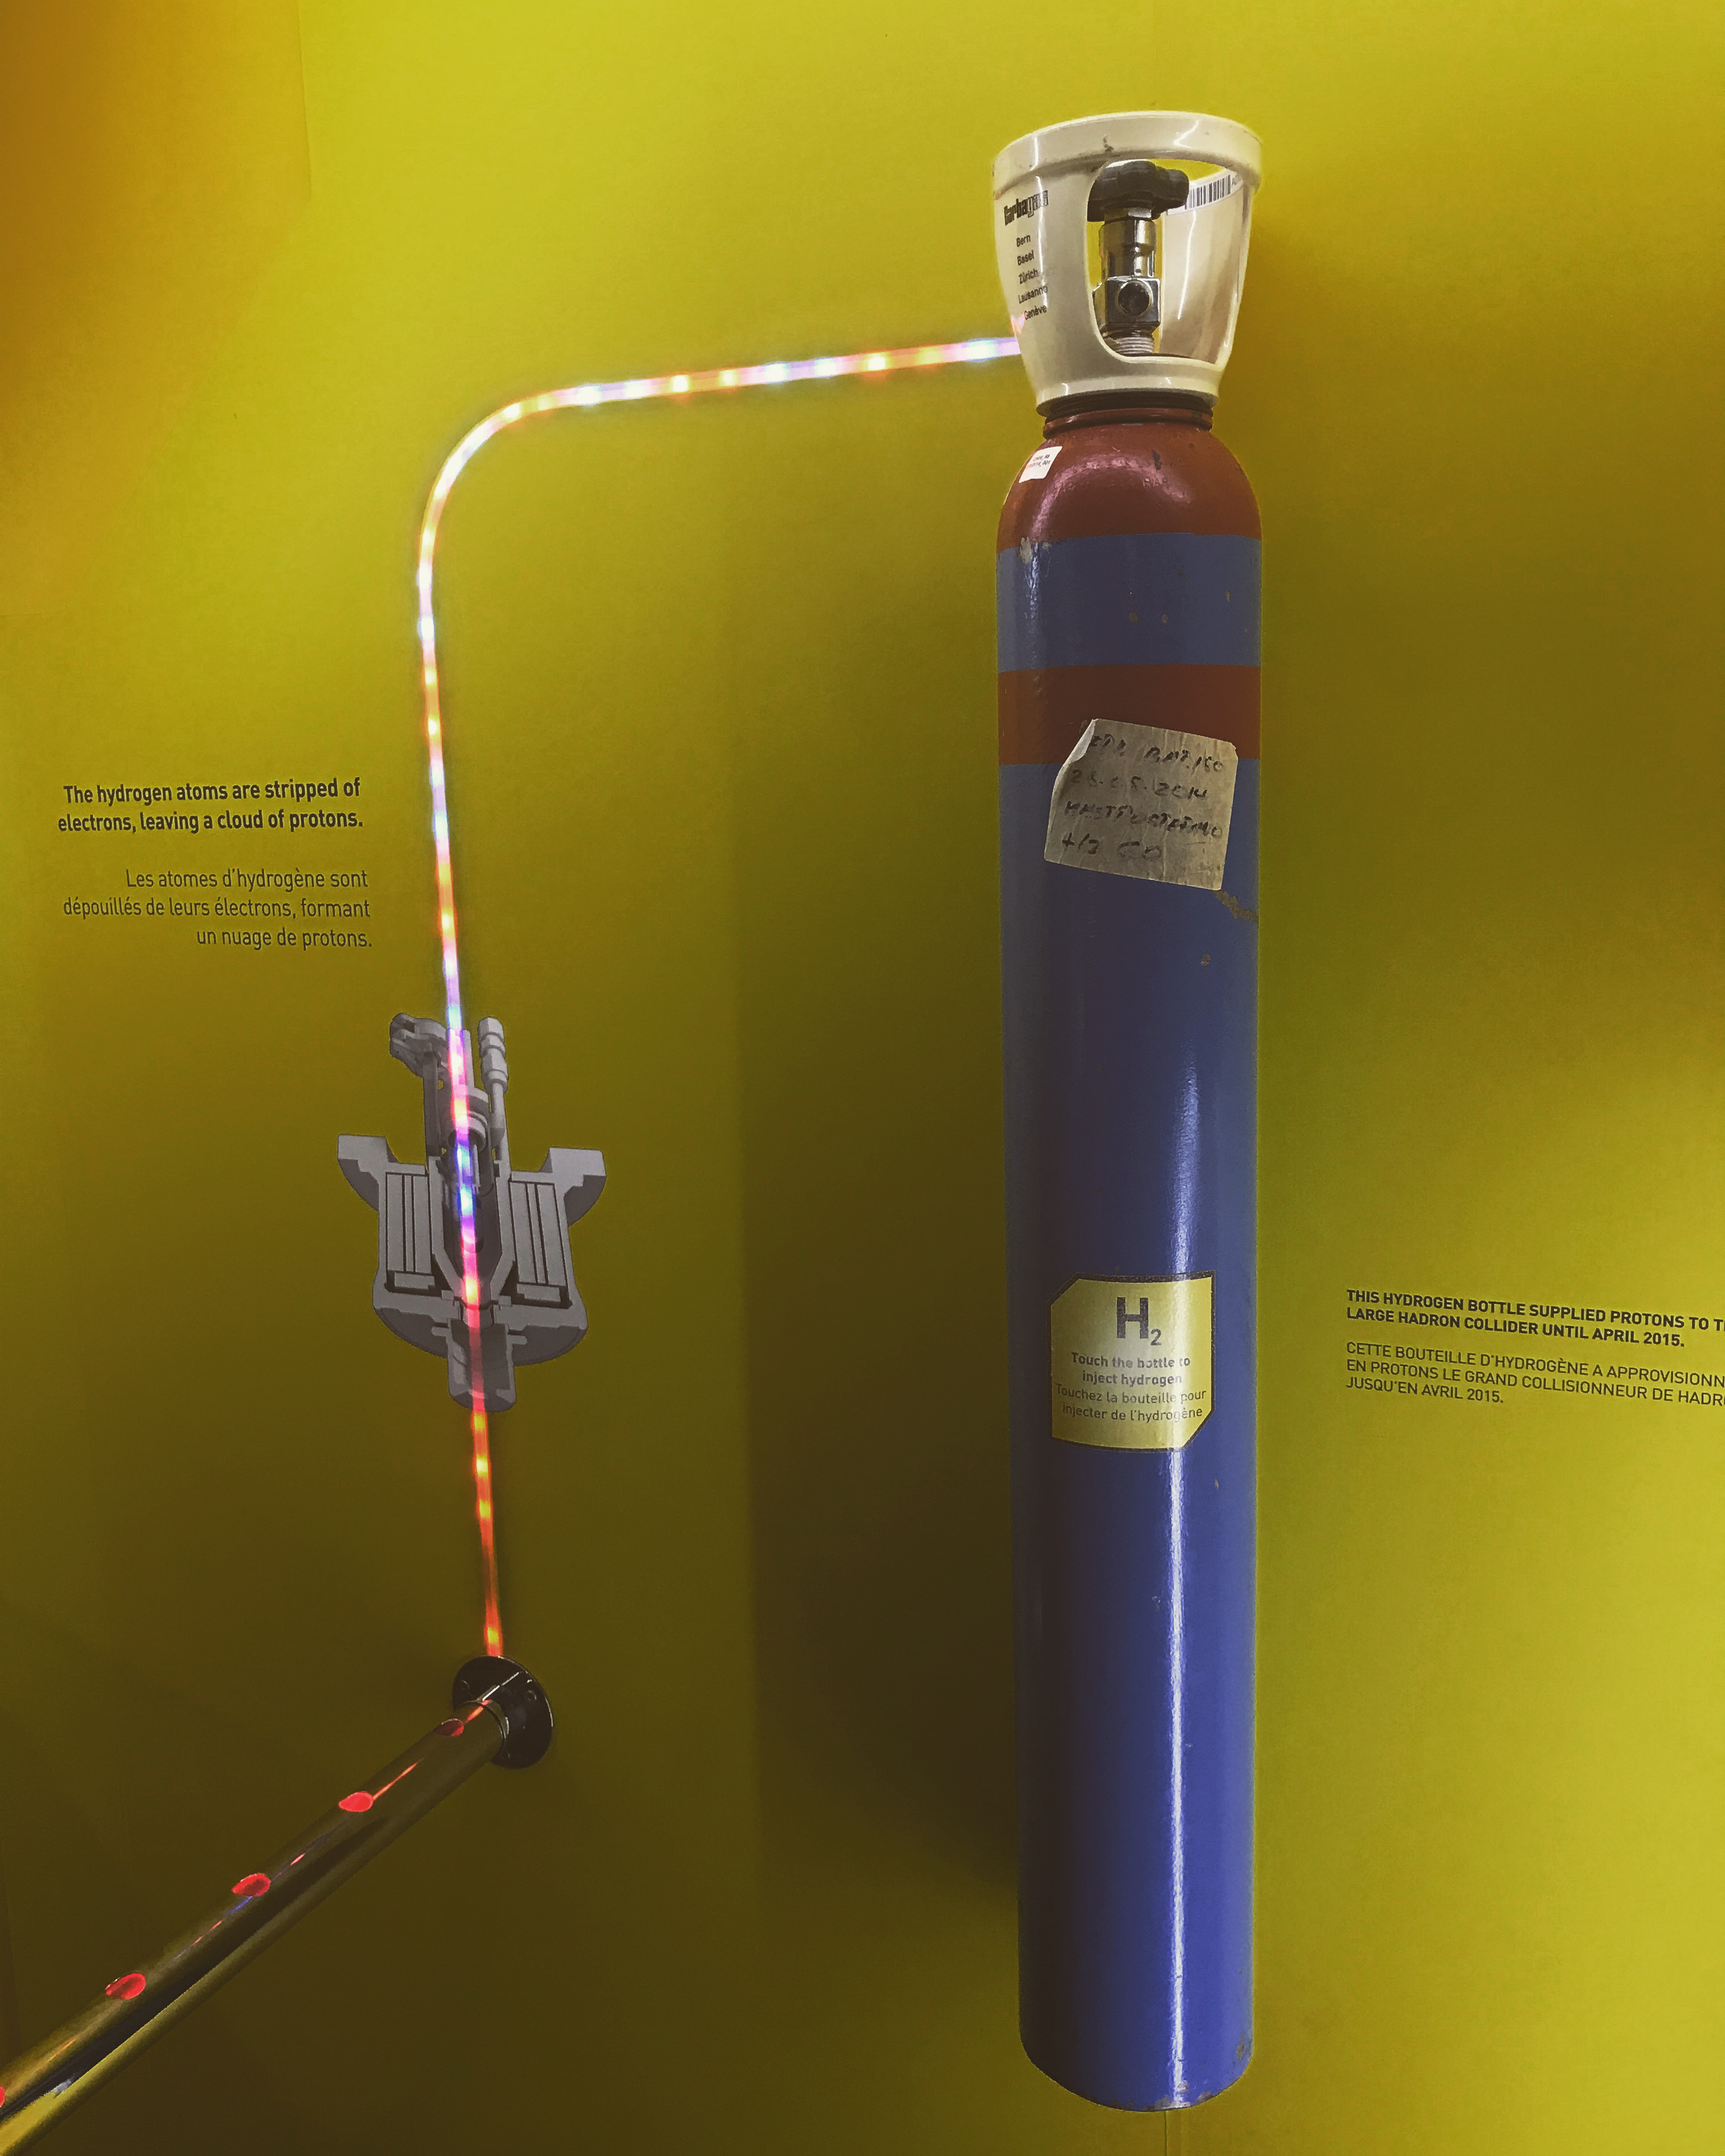
\includegraphics[scale=0.038]{fig/H2Bottle.JPG}
% 	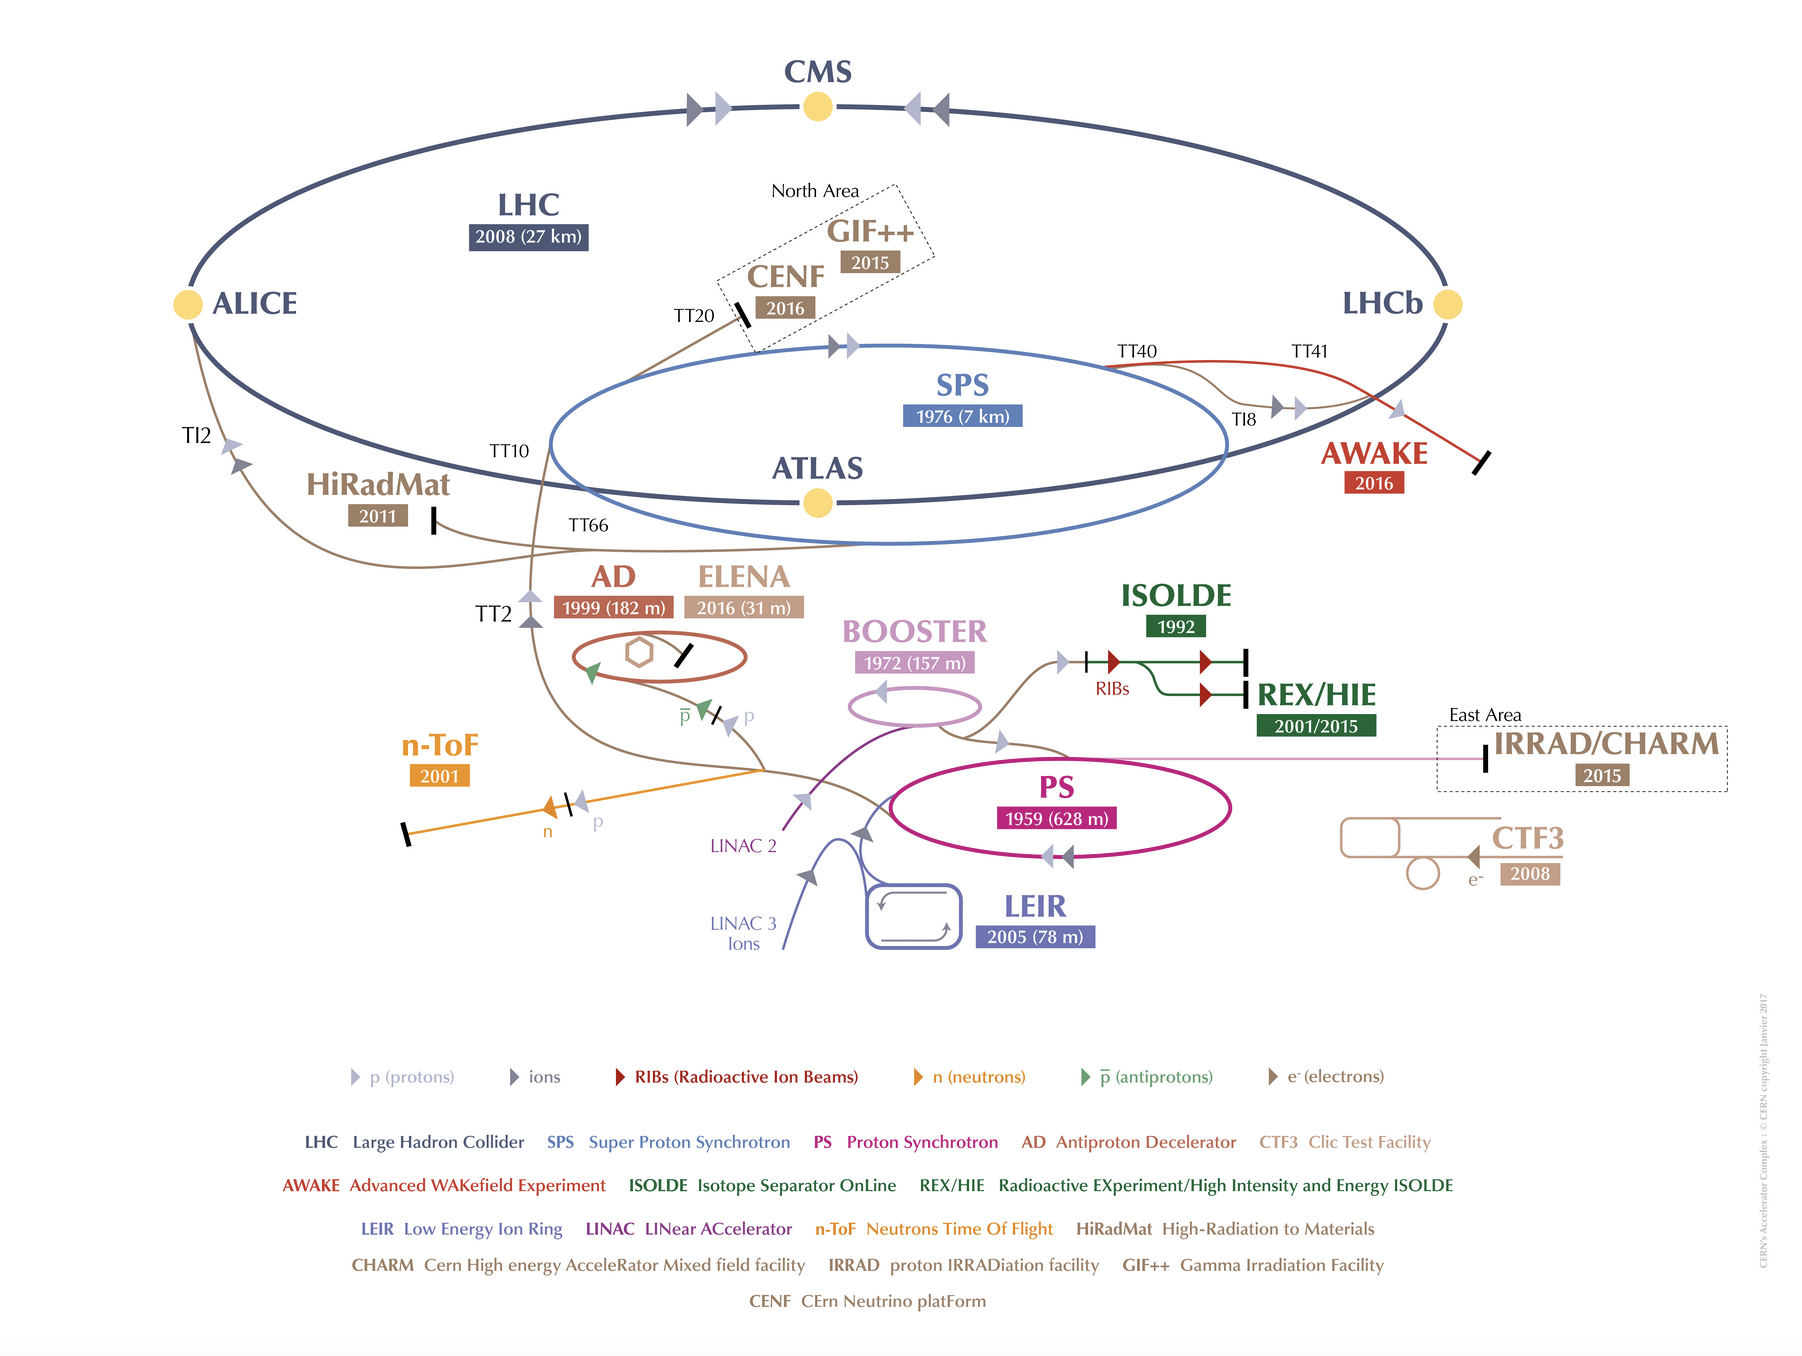
\includegraphics[scale=0.26]{fig/CERNAcceleratorComplex.png}
% 	\caption{The protons used for collisions begin their journey from a bottle of hydrogen \cite{LHCbottle} and they are sent through a series of accelerators to ramp up particle beam energies to 6.5 TeV  }
% 	\label{fig:accelerator_complex}
% \end{figure}

\begin{figure}[!htbp]
	\centering
	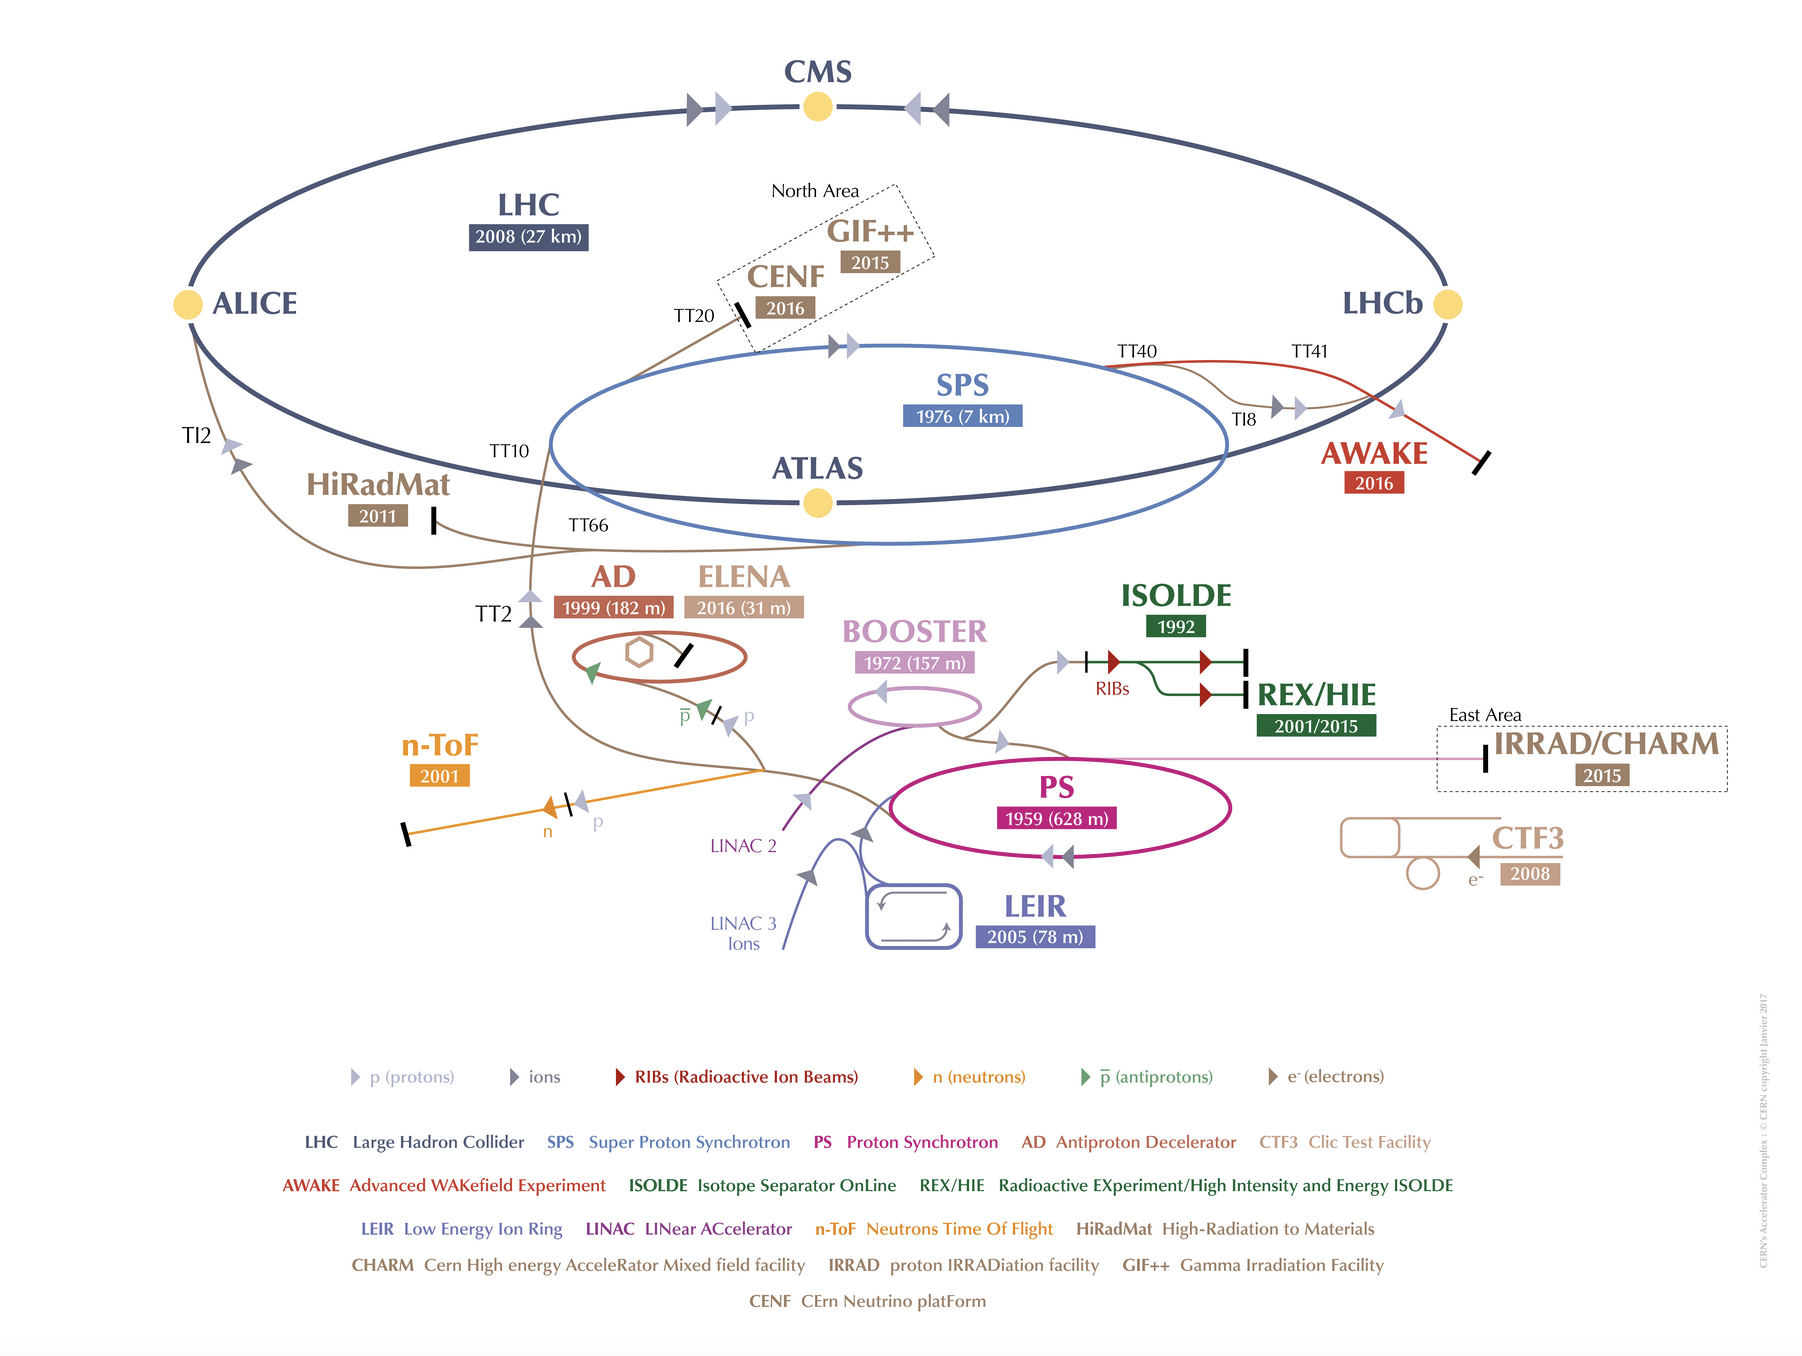
\includegraphics[scale=0.5]{fig/CERNAcceleratorComplex.png}
	\caption{The CERN Accelerator complex has a series of accelerators that ramp up particle beam energies to 6.5 TeV in Run II.}
	\label{fig:accelerator_complex}
\end{figure}

\subsubsection{Collider Design Fundamentals}

Creating new particles and probing the underying structure of matter requires energy and momenta - quantities whose magnitude are dictated by Einstein's equation on Mass-energy equivalence $E^2=(mc^2)^2+(pc)^2$ and de-Broglie's relation. The LHC achieves high energies through its near perfectly circular design with a large radius, $r\approx4$-km. In this section we discuss the advantages and disadvantages of these design choices to guide  future colliders.

Circular colliders have a distinct advantage over linear ones. The first one is high collision rates. Particle beams could circulate over the 27-km ring at a rate of 11 kHz, for many hours allowing it to achieve the highest nominal collision rates at 40 MHz. This collision rate is calculated by multiplying the number of bunches times their revolution frequency - which are experimentally modified. Linear colliders, on the other hand, have the disadvantage of having to be refilled with bunches at each collision. 

% The average crossing rate = number of bunches * revolution frequency = 2808 * 11245 = 31.6 MHz.  Times 19 events per crossing at nominal luminosity gives us our 600 million inelastic events per second." \cite{collisionRatePop}}. 

% To create new particles and to probe the underlying structure of atom, we would need energy. The higher the energy we could produce, the higher the masses of the particles we could probe, the better the resolution \footnote{Energy is related to mass: 
% \begin{equation}
%     E = mc^2 
% \end{equation} 
% where $c$ is the speed of light. For us to probe the underlying structure of matter in better detail, we would also require finer wavelengths or higher momenta as shown with de-Broglie relation given by:
% \begin{equation}
%    \lambda = \frac{h}{p}
% \end{equation} 
% where $h$ is $h = 6.626 * 10^{-34} Js$ and $p$ is the particle momentum.}.

 The drawbacks \cite{Ferrario:2020zwm, Andrews:2022nza} for ciruclar colliders mainly come from synchrotron radiation loss. Circulating charged particles means there are energy losses with the following proportionality rate:
\begin{equation}
    P \propto \frac{q^2}{m^4 R^2}.
\end{equation}
Second, a large magnetic magnetic field is also required to maintain the circular path of the particles. Assuming an idealized homogeneous dipole oriented along the particle orbit, the magnetic field strength required is:
\begin{equation}
    |\vec{B}|= \frac{|\vec{p}|}{qcR}.
\end{equation}

For the LHC, these radiation losses are mitigated by having a large-radius accelerator. This also simultaneously contributes to having a larger magnetic field. Interestingly, the LHC uses the repurposed tunnels of the Large Electron Positron (LEP) Collider, the largest radius of any collider in the world.

The LHC from the name itself, collides hadrons which are composite particles made of two or more quarks. Most hadrons are unstable, in contrast with Protons, or heavy elements like lead (\textbf{Pb}) or gold that have long lifetimes making them good choices for particle collisions. In our analysis, we only examine proton-proton collisions. A complication that arises from colliding a composite particle, is that the full momentum is shared by the actual interacting particles. Electrons, which are point-particles are much simpler, i.e. we know exactly the energy of the initial state, i.e. if we were to collide, an electron and a positron. In their simplest representation, protons (uud), are composed of two up quarks and a down quark and gluons which bind these components together. In addition, sea quarks arise from the energy of gluon splitting. The constituent quarks or gluons, collectively known as partons carry only a fraction of the energy and this fraction is determined by the parton distribution functions. Parton distribution functions give the probability to find partons carrying a fraction x of the proton's total momentum. Apart from the primary collision event or the hard scattering event, there are also softer scattering events which are called underlying events. 

The LHC program transitions to the High-Luminosity (HL-LHC) phase beginning in Run3 and ends by around 2040. At this time, a Future Circular Collider (FCC) is expected to push the energy and intensity frontier of particle colliders, with the aim of reaching collision energies up to 100 TeV \cite{Blondel:2021ema}. Figure~\ref{fig:hl-lhc} shows the LHC and HL-LHC scheduled in different phases, while Figure~\ref{fig:lhcschedule} shows the updated LHC schedule accounting for the delays due to the COVID-19 pandemic.

\begin{figure}[!htb]
	\centering
	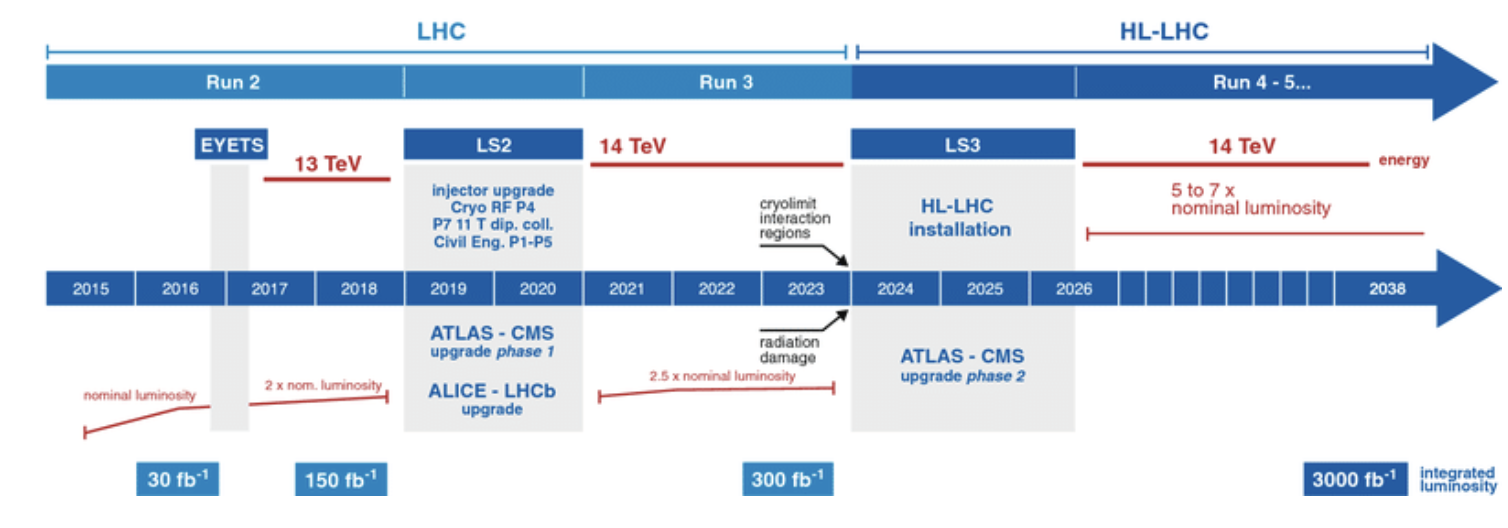
\includegraphics[scale=0.6]{fig/LHC-schedule.png}
	\caption{An overview of the LHC schedule from Run2 onwards before the COVID-19 pandemic delays.}
	\label{fig:hl-lhc}
\end{figure}


\begin{figure}[!htb]
	\centering
	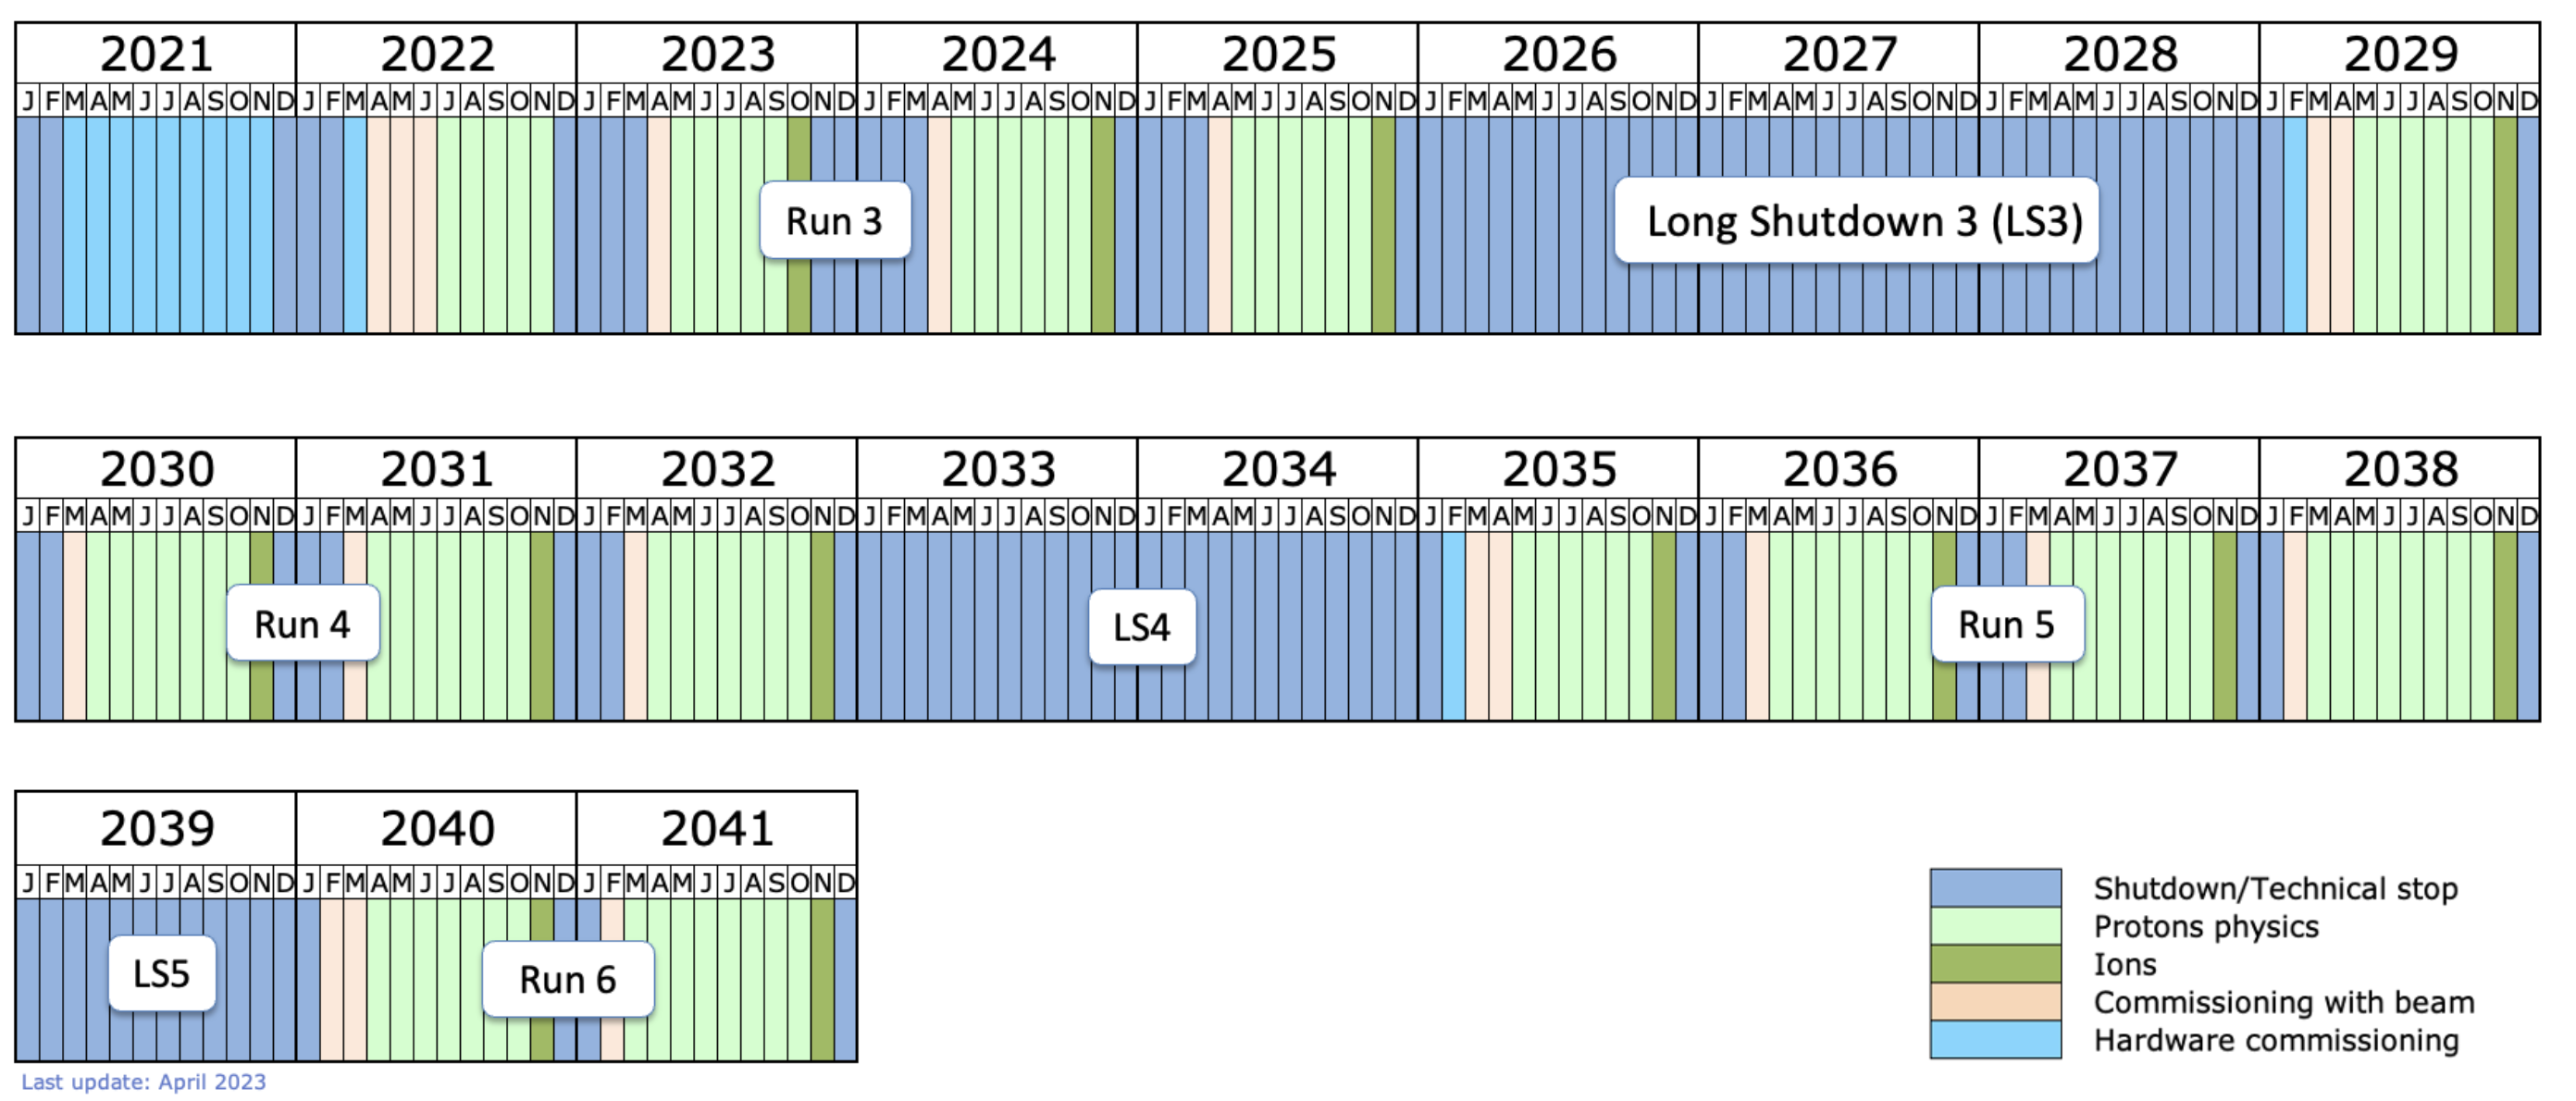
\includegraphics[scale=0.3]{fig/HL-LHC.png}
	\caption{An updated schedule of the LHC accounting for the delays due to the COVID-19 pandemic (Credits: LHC-Commissioning)}
	\label{fig:lhcschedule}
\end{figure}

\section{LHC Schedule, Beam Performance and Pileup}

The LHC operates in production cycles consisting of Runs and Long Shutdowns (LS). In Run 1 of the LHC, which took place from 2010-2012, the LHC operated at 7-8 TeV centre-of-mass energy. This was followed by a 3-year Long Shutdown period where upgrades and repairs were performed. Run 2 started in the summer of 2015 and ended in 2018. During this time, the LHC delivered $163.54$~\fbinv  of data at 13 TeV which surpassed the design luminosity goal of $L = 10^{34}$ cm$^{-2}$s$^{-1}$. This number is generally referred to as the integrated luminosity, $L = \int \mathcal{L} dt$.

The luminosity is different from the collision rate. The proton beam bunches cross at 40 MHz, but not all of the protons within the beam collide as the proton bunches have to be focused into a smaller cross-section.In terms of the beam parameters, the instantaneous luminosity is defined as 

% One could think of luminosity as a beam characteristic. It describes how much of the protons could be squeezed in a beam of a given cross-section. The more particles squeezed in a smaller space, the greater the luminosity. 
\begin{equation} \label{eq:beamParam}
    \mathcal{L} = \frac{N^2_{b}*fn_{b}}{4\pi\sigma^{*}_{x}\sigma^{*}_{y}}F,
\end{equation}

where $N_{b}$ is the beam intensity or the number of protons/bunch; $n_{b}$ is the number of bunches, $f$ is the revolution frequency of the protons, $\sigma^{*}_{x,y}$ are the transverse RMS beam widths at the interaction point; and $F$ is a geometric loss factor that accounts for crossing angle, shape, and longitudinal beam size.

% \footnote{At the LHC this is at 11 kHz with a beam energy of 6.5 TeV}

For a given physics cross-section, the total number of events produced is related to the Luminosity as such:

\begin{equation}
    N_{\textnormal{events} } = L \sigma.
\end{equation}
% To get more events therefore requires a more focused beam which translates to a requirement of higher luminosity.

While higher luminosities provide us more data, it comes with challenges. In each of the proton bunch crossing, multiple simultaneous interactions occur. This problem is known as \textbf{pileup}. This problem can be mitigated by attempts to reconstruct the primary collision vertex but there are also other spurious events that could lead to problems in the reconstruction of physics objects. Additionally, out-of-time pileup can also occur. These arise from collisions coming from prior or later bunch crossings. These factors are major driving forces in the design of CMS algorithms and future detector upgrades. 

% \begin{figure}[tbp!]
% \begin{center}
% 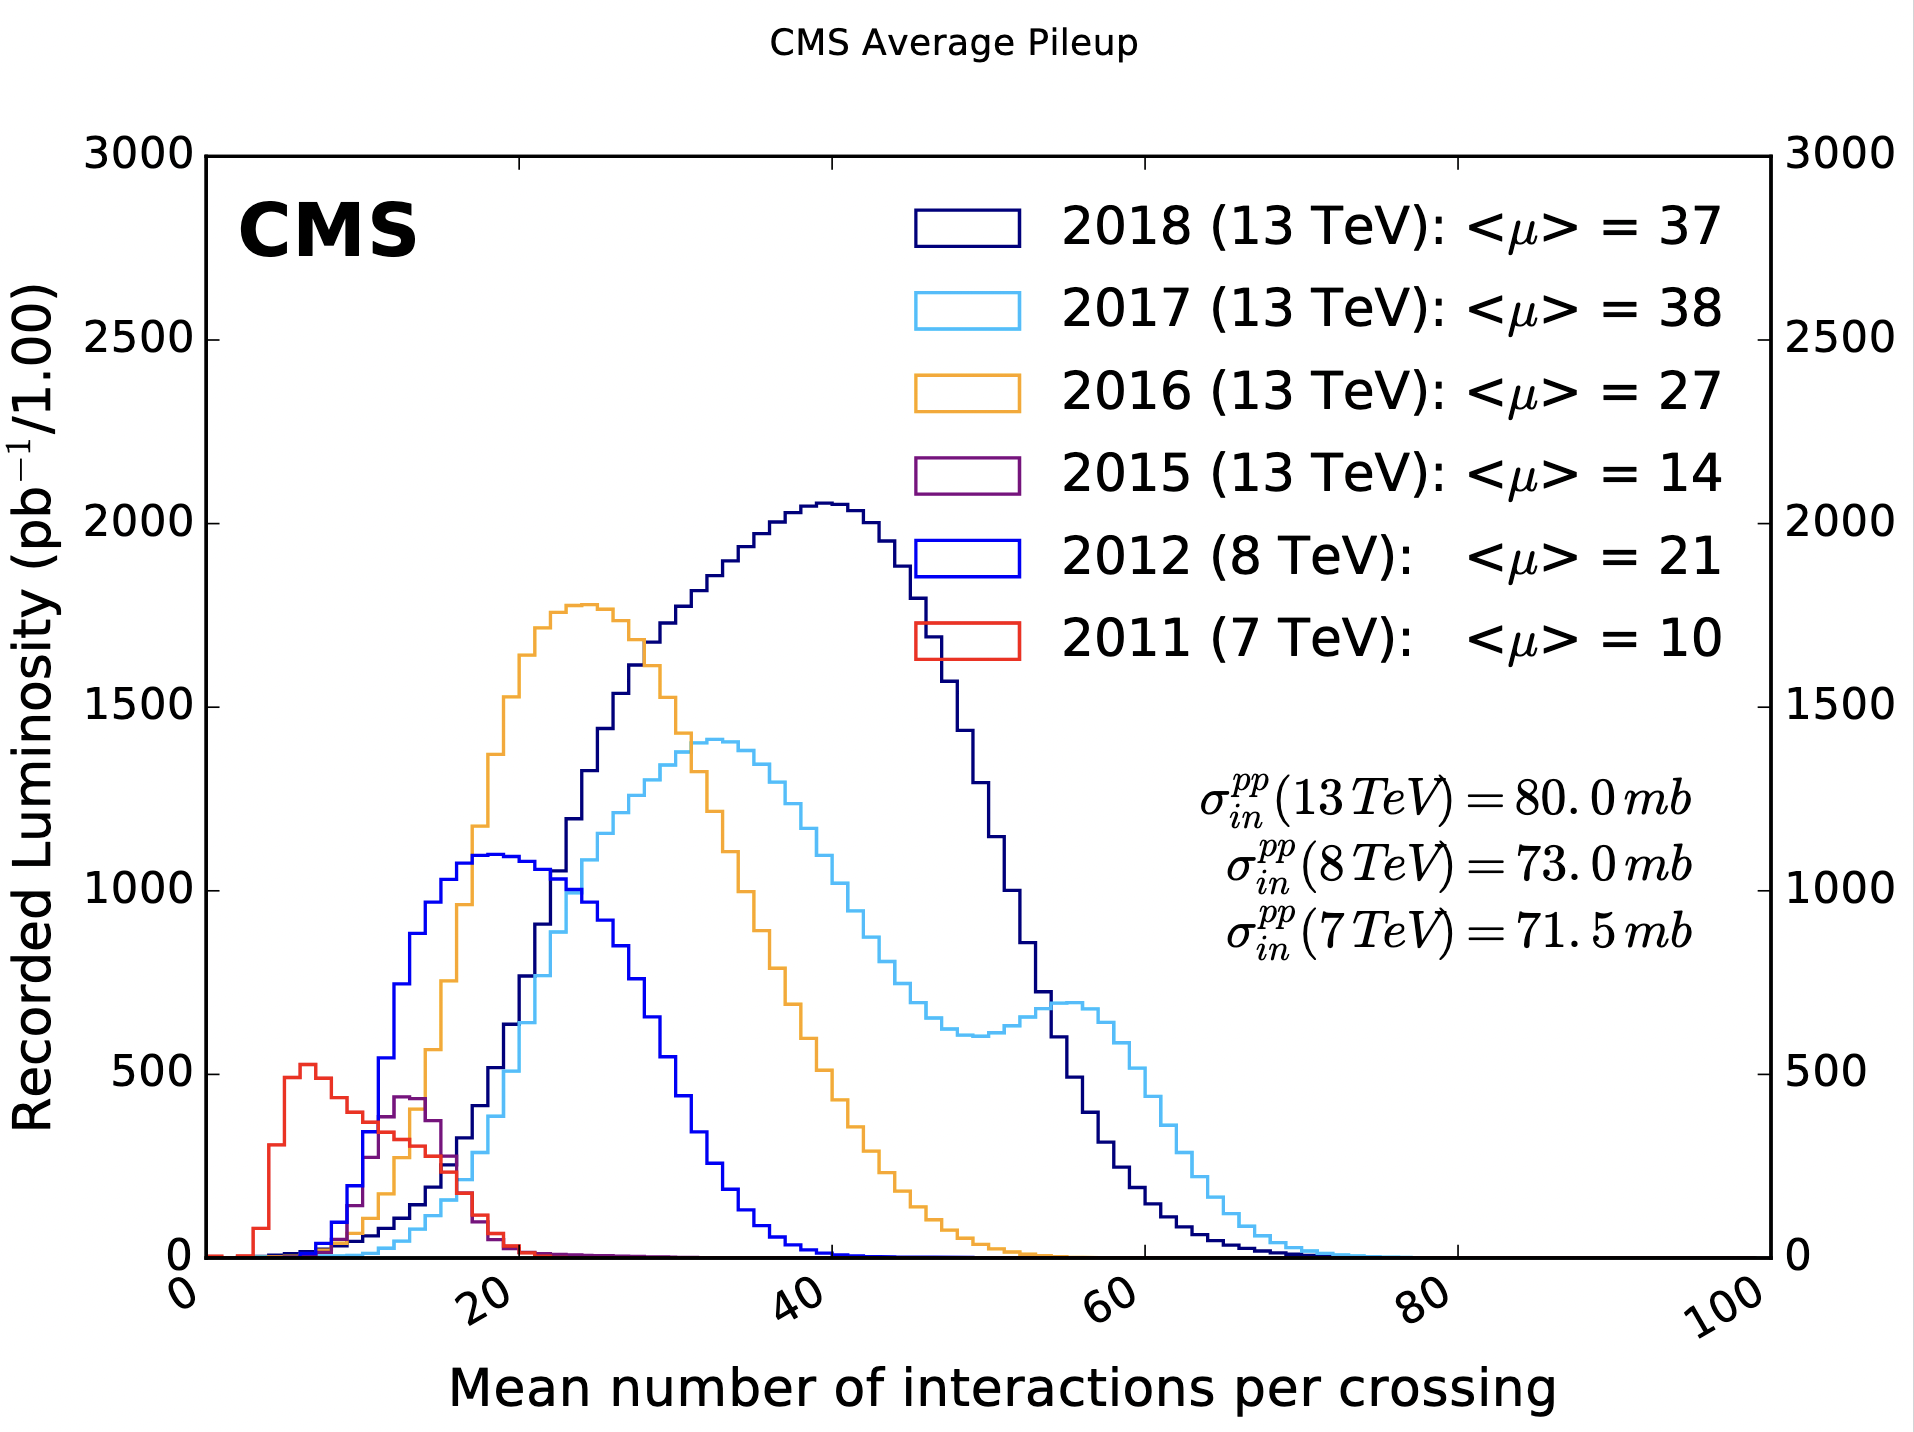
\includegraphics[angle=0,width=0.45\textwidth]{fig/PileUpRun2On.png}
% 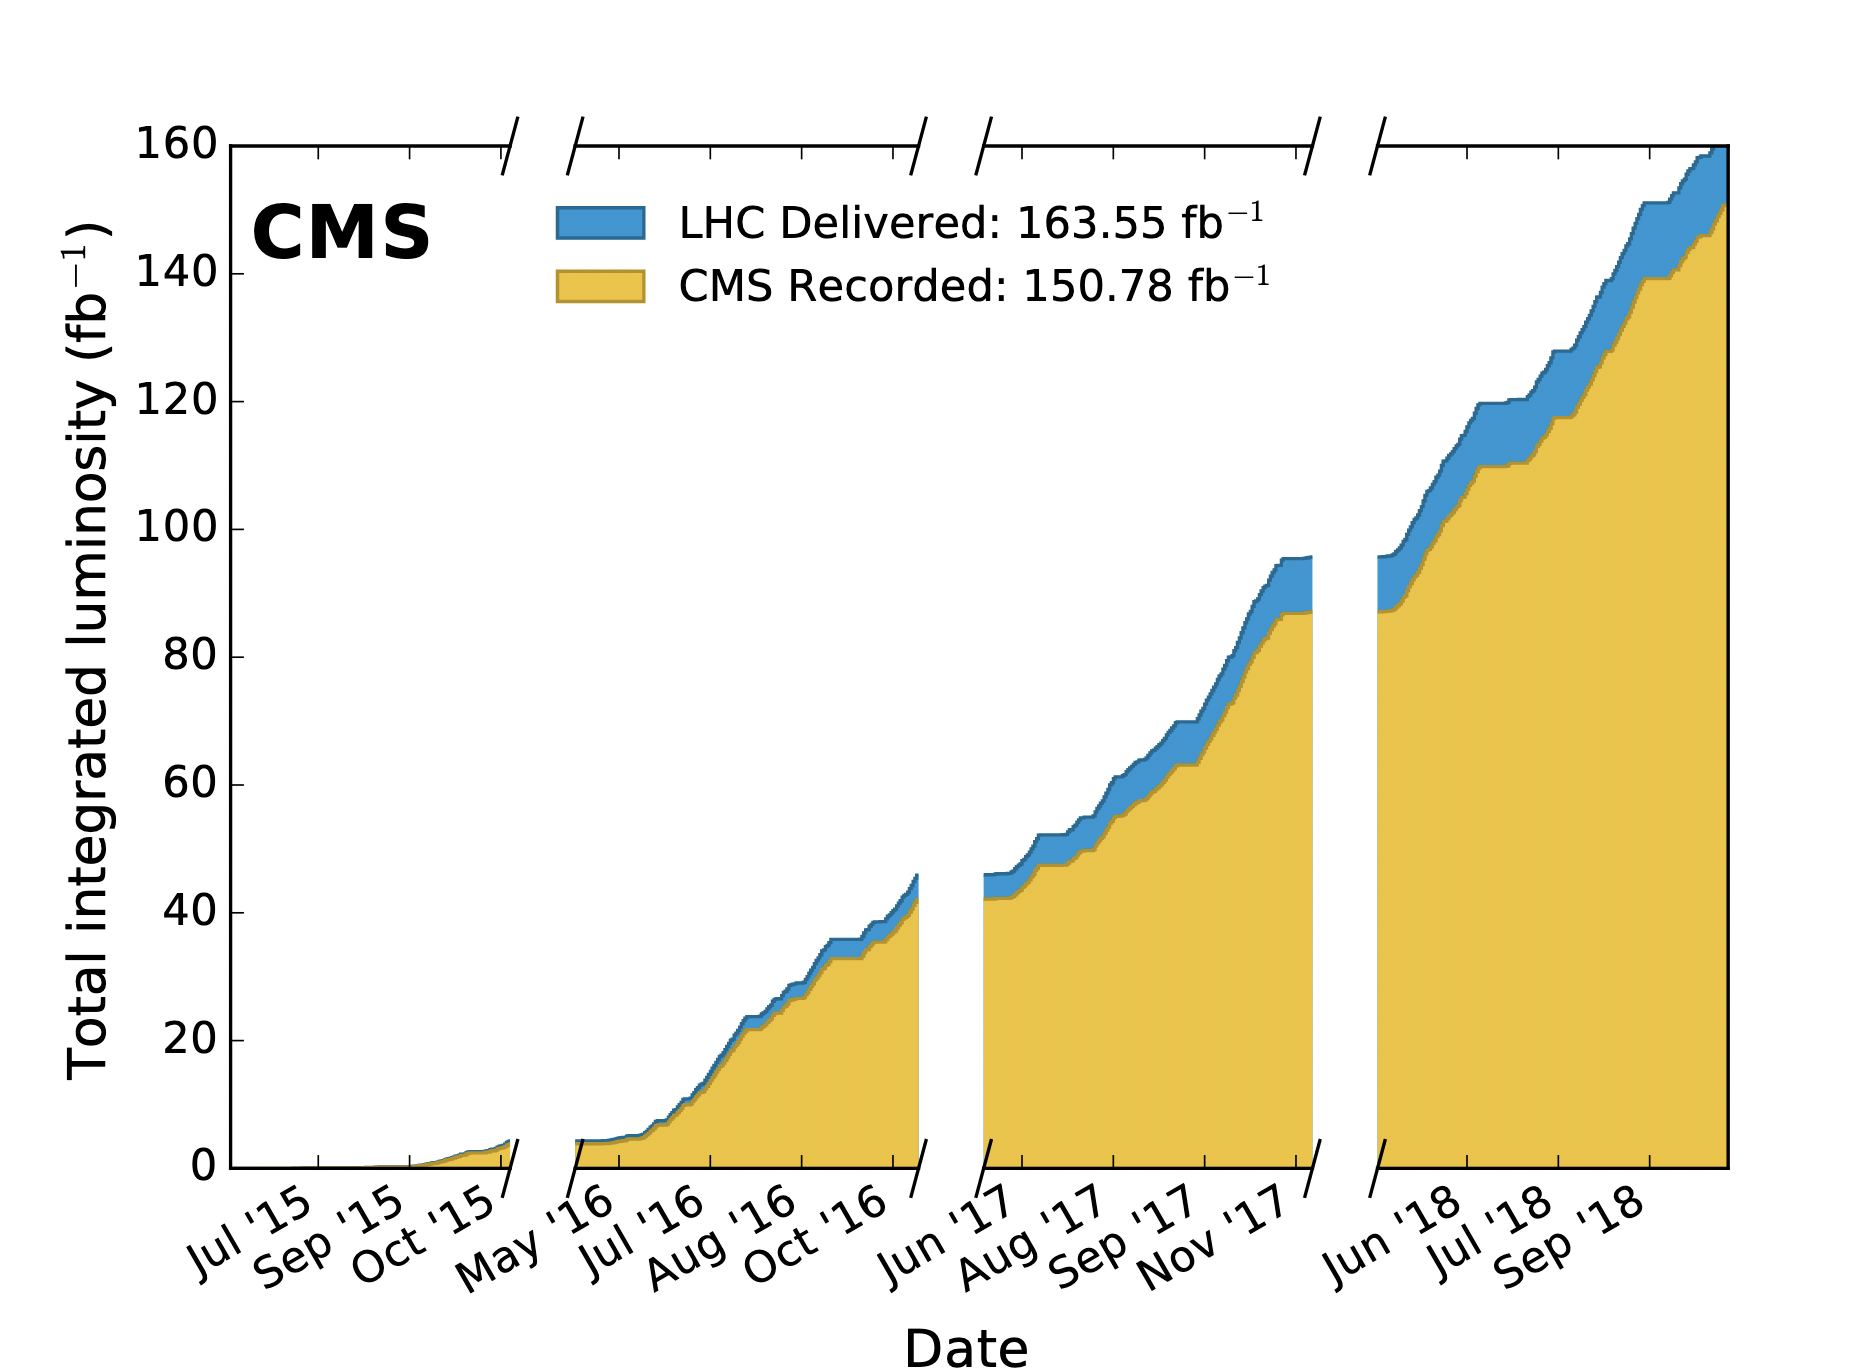
\includegraphics[angle=0,width=0.45\textwidth]{fig/LuminosityRun2.png}
% \end{center}
% \caption{Pileup and Luminosity information from Run II from CMS Lumi Public Results.
% }
% \label{fig:LHCBeam}
% \end{figure}

\begin{figure}[tbp!]
\begin{center}
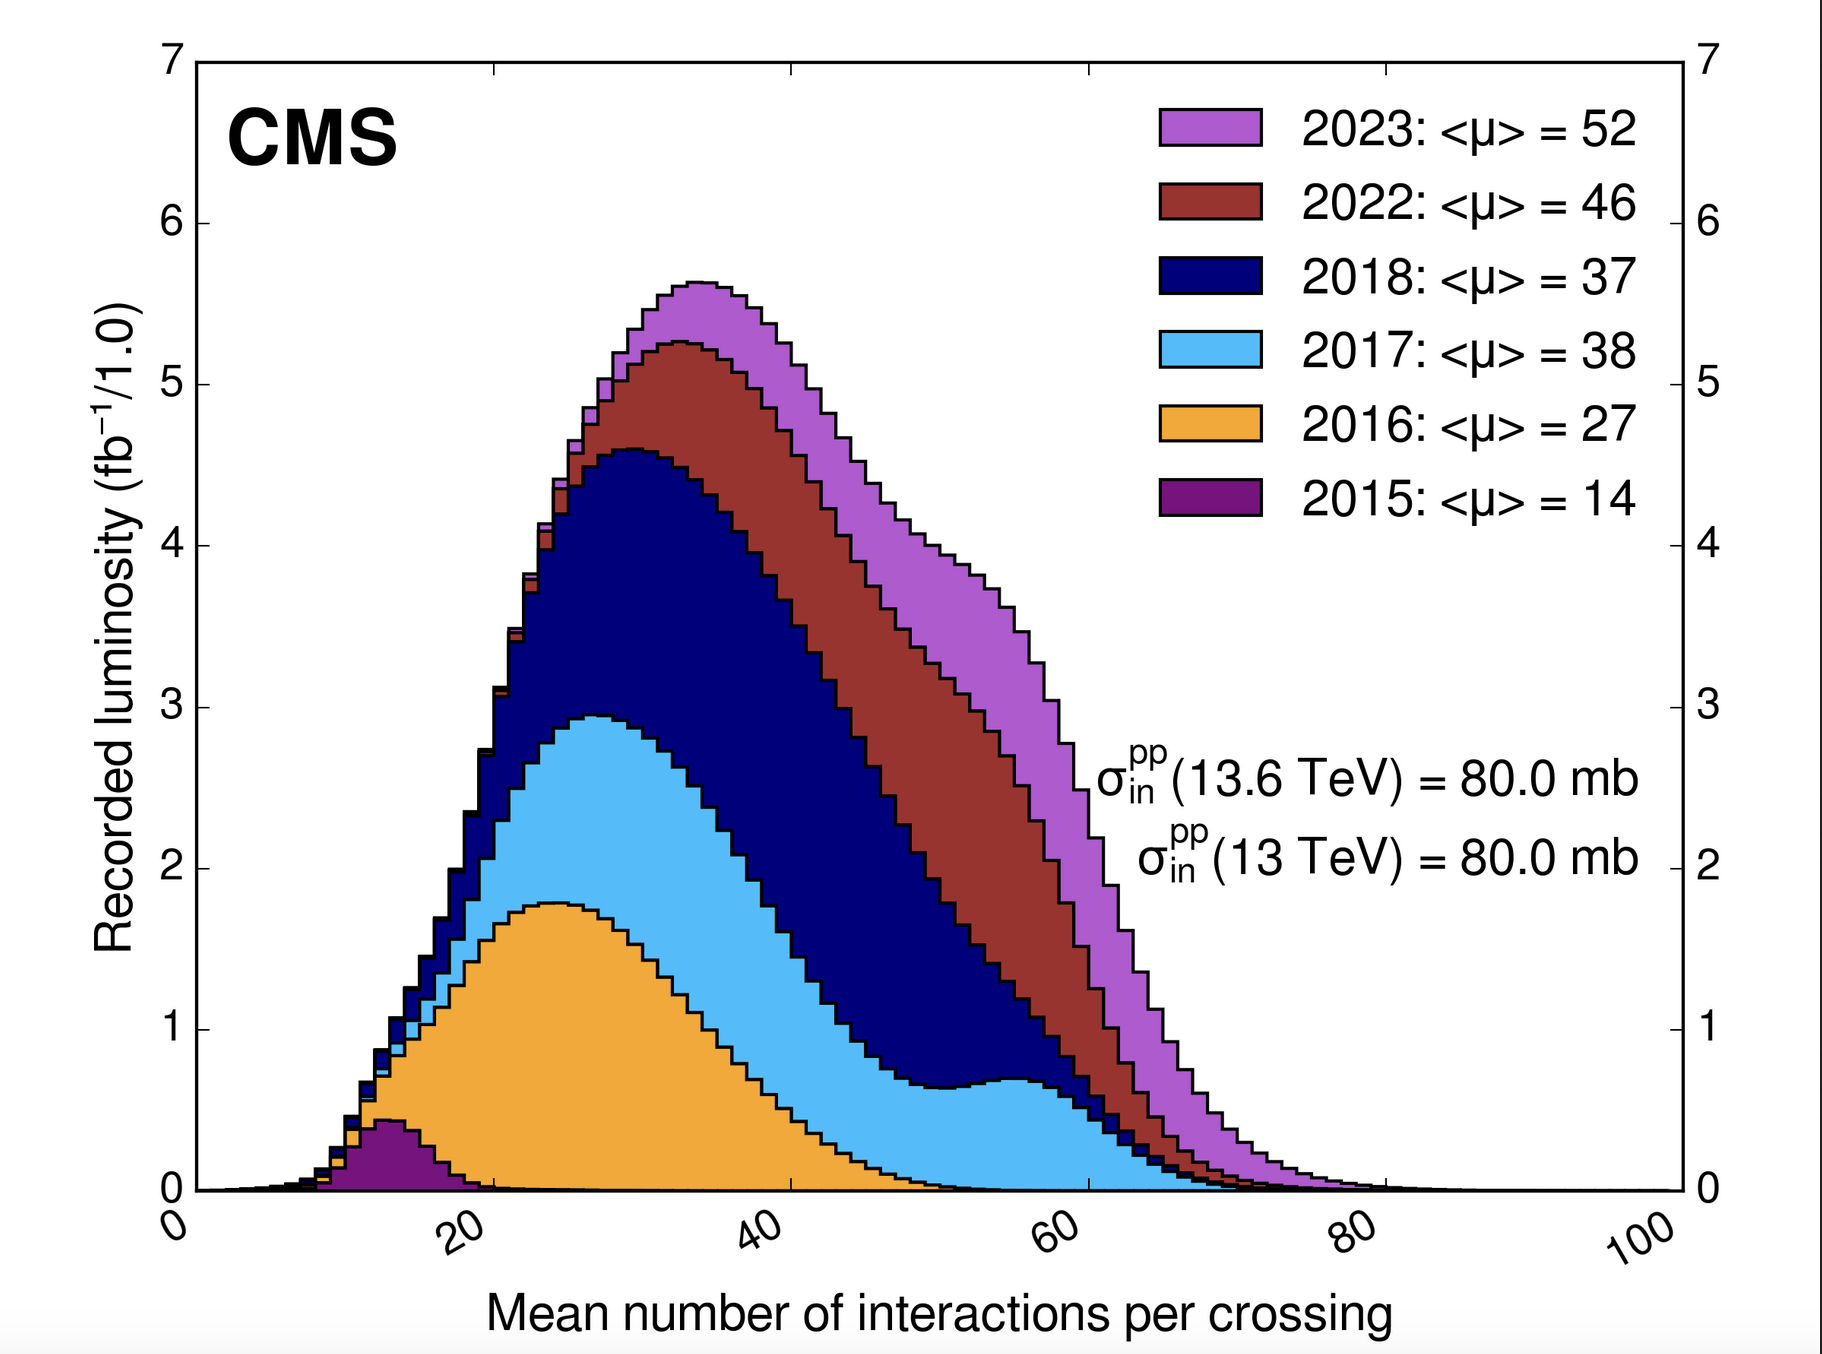
\includegraphics[angle=0,width=0.45\textwidth]{fig/PileupAcrossTheYears.png}
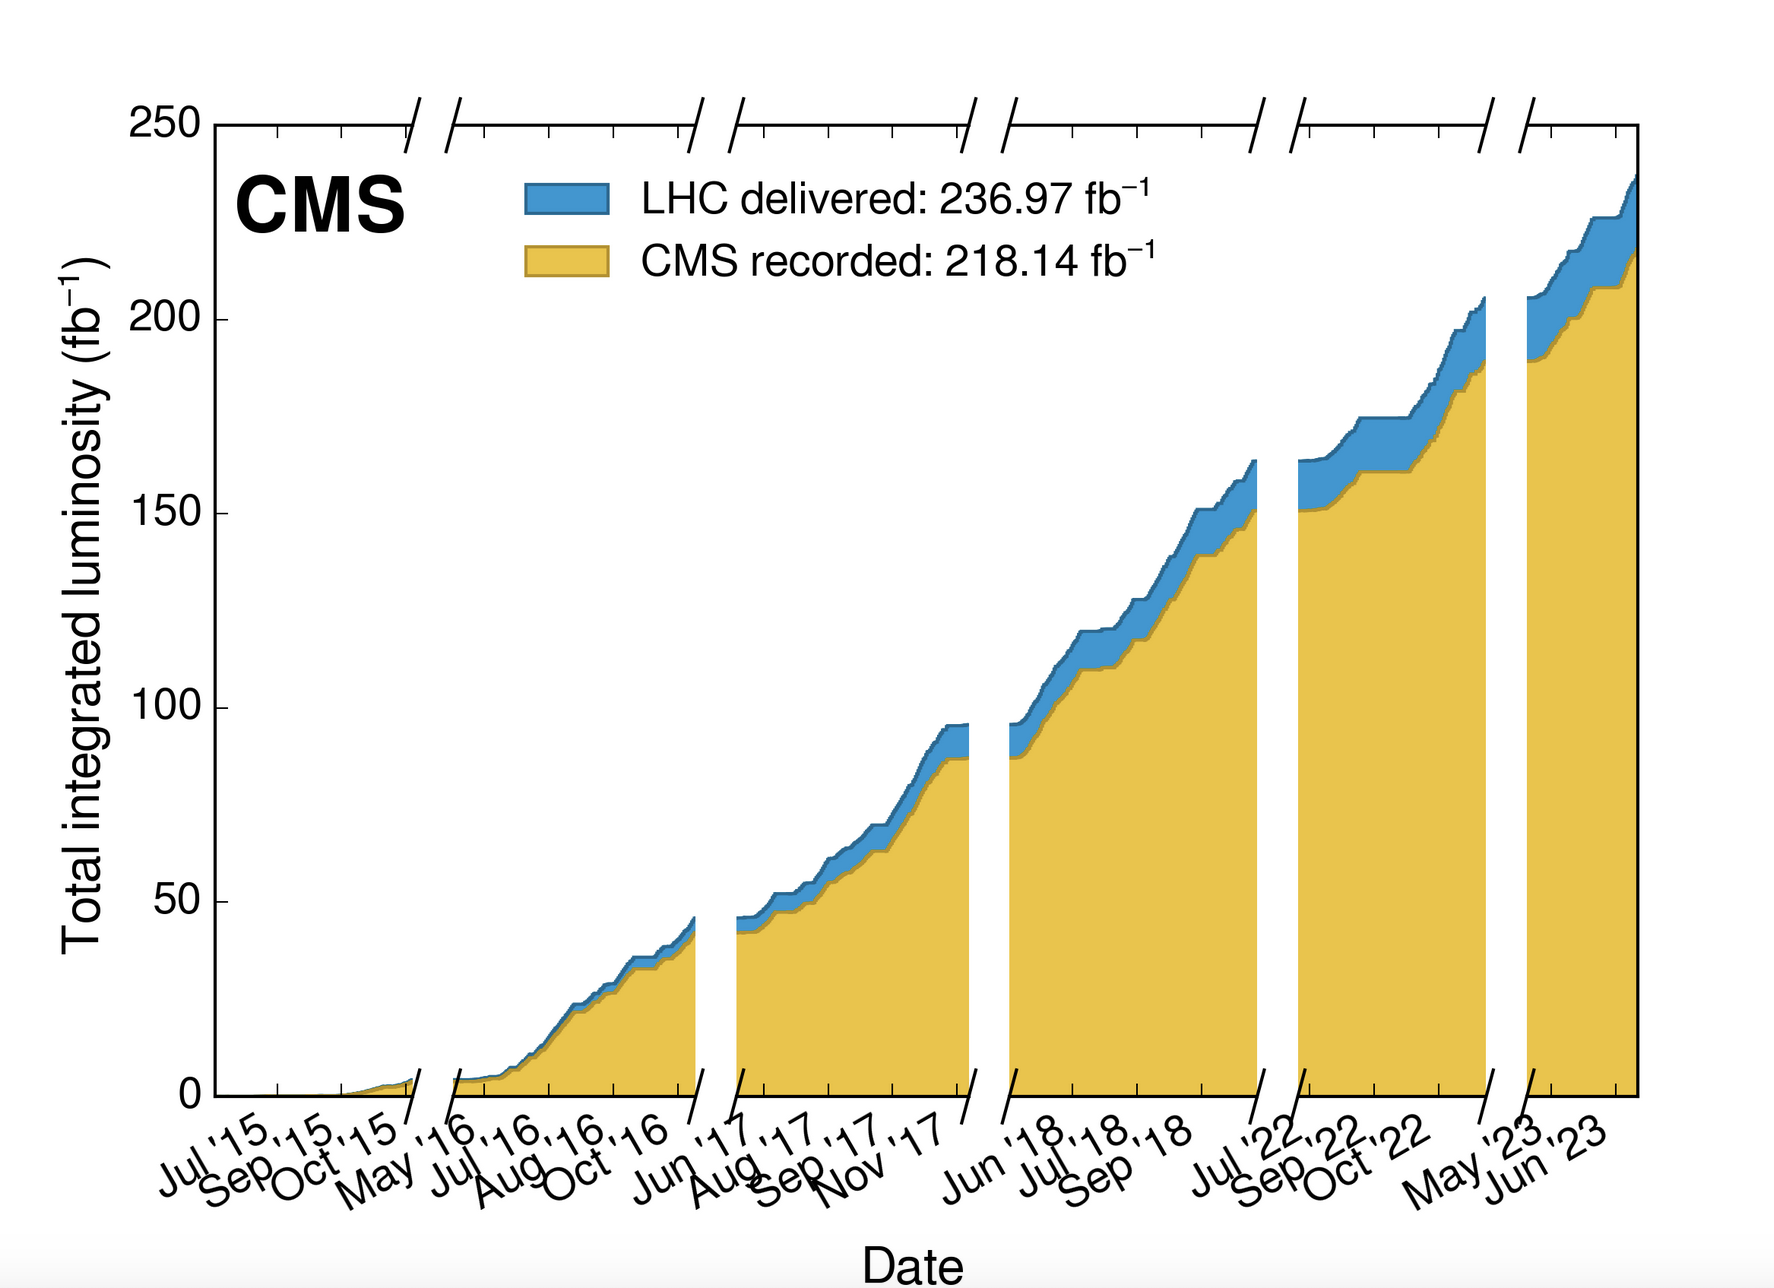
\includegraphics[angle=0,width=0.45\textwidth]{fig/LuminosityAcrossTheYears.png}
\end{center}
\caption{The mean number of pileup or inelastic interactions per proton bunch crossing in data
for proton-proton (pp) collisions for various years (left). A total inelastic pp collision
cross section of 69.2 mb is chosen~\cite{CMS:2020ebo}. The Luminosity is shown for various time with white spaces for periods the LHC is not operating (right).}
\label{fig:LHCBeam}
\end{figure}






% idealized homogeneous dipole oriented along the particle orbit, we define the condition for
% a perfect circular orbit as equality between these two forces; this yields the following condition for the
% idealized ring: p
% e = B · ρ, 
%%%
% How many times can proton beams circle around the LHC? 
%
%
%%%

% \feynmandiagram [horizontal=a to b] {
%   i1 -- [fermion] a -- [fermion] i2,
%   a -- [photon] b,
%   f1 -- [fermion] b -- [fermion] f2,
% };

% Linear accelerator\cite{Holzer:2016lud}


%%%%%
% - The Higgs Discovery: https://www.youtube.com/watch?v=so2nCu2Jkbc 
% - How does the LHC work: https://www.youtube.com/watch?v=oWpy0SAAI6E 
% - How does the 
% - https://www.nobelprize.org/prizes/physics/2013/summary/ 
% The Nobel Prize in Physics 2013 was awarded jointly to François Englert and Peter W. Higgs "for the theoretical discovery of a mechanism that contributes to our understanding of the origin of mass of subatomic particles, and which recently was confirmed through the discovery of the predicted fundamental particle, by the ATLAS and CMS experiments at CERN's Large Hadron Collider" 
%%%%%

% - Motivation 
% - the large 
% - proton journey starts from a bottle
% \cite{Evans:2008zzb} \\
% - accelerator complex \cite{Bulletin:1255151} \\ 

% -------------------------------
% - Proton-proton collisions, COM and Luminosity \cite{Bulletin:1255151} \\
% - ALICE \cite{ALICE:2008ngc} \\
% - CMS  \\
% - ATLAS \cite{ATLAS:2008xda}\\
% - LHCb \cite{LHCb:2008vvz} 
% - LHC schedule, CMS mass energies, pileup mitigation \cite{CMS:2020ebo}
% \section{CMS Experiment - Detector}
% The CMS detector\cite{CMS:2008xjf} \\ 

% Copy paste chunks from here:
% https://twiki.cern.ch/twiki/bin/viewauth/CMS/Internal/PubDetector

% Maybe add something from the TDR  \cite{CMS:2008xjf}
% ----------------------------------
% \subsection{Detector Coordinates}
% Nice discussion by Afiq \cite{Anuar:2019rft}
% \subsection{Particle Interaction with Matter}
% Mike has a very nice discussion here\cite{Andrews:2022nza}
% \subsection{Subdetectors}

% \subsection{CMS ECAL}

% % \subsection{Magnet}
% % \subsection{Inner Tracking System}
% precision tracking \cite{CMS:2018wqs}
% \subsubsection{Electromagnetic Calorimeter}
% Photons, calorimeter, lead-tungstate module 
% General description of passage of particles in materials \cite{ParticleDataGroup:2018ovx} \\
% \subsubsection{Hadron Calorimeter}

% Upgrade \cite{Cooper:2016kef}
% % \subsection{Muon System}
% Design and performance of the wedges\cite{CMSHCAL:2007zcq}

\section{CMS Experiment and Its Subdetectors}~\label{sec:CMSDetector}
The CMS detector (Figure~\ref{fig:CMSdetectorCutaway}), is one of general-purpose detectors of the LHC which collects the data generated at the CMS interaction point found in P5 in Cessy, France. The detector has a series of concentric cylindrical layers which comprise the Barrel region of the detector. To capture collision products going in the more forward regions, at angles moving closer to the beam line, Endcap detectors are also constructed. These layers hermetically seal the central collision point.

The CMS uses a coordinate system that is centered at nominal interaction point which is found halfway through the cylinder axis of the detector. The z-axis goes through the beam pipe, and the radial coordinate, r is measured from this axis. The angular coordinates $\phi$ and $\eta$ are defined as follows, $\phi$ corresponds to the azimuthal angle or the horizontal angle going clockwise around the z-axis, and $\eta$ is the pseudorapidity which is related to the angle $\theta$ by the equation (see Figure~\ref{fig:etatheta}),

\begin{equation}
    \eta = -ln (tan(\theta/2)).
\end{equation}

\begin{figure}[tbp!]
\begin{center}
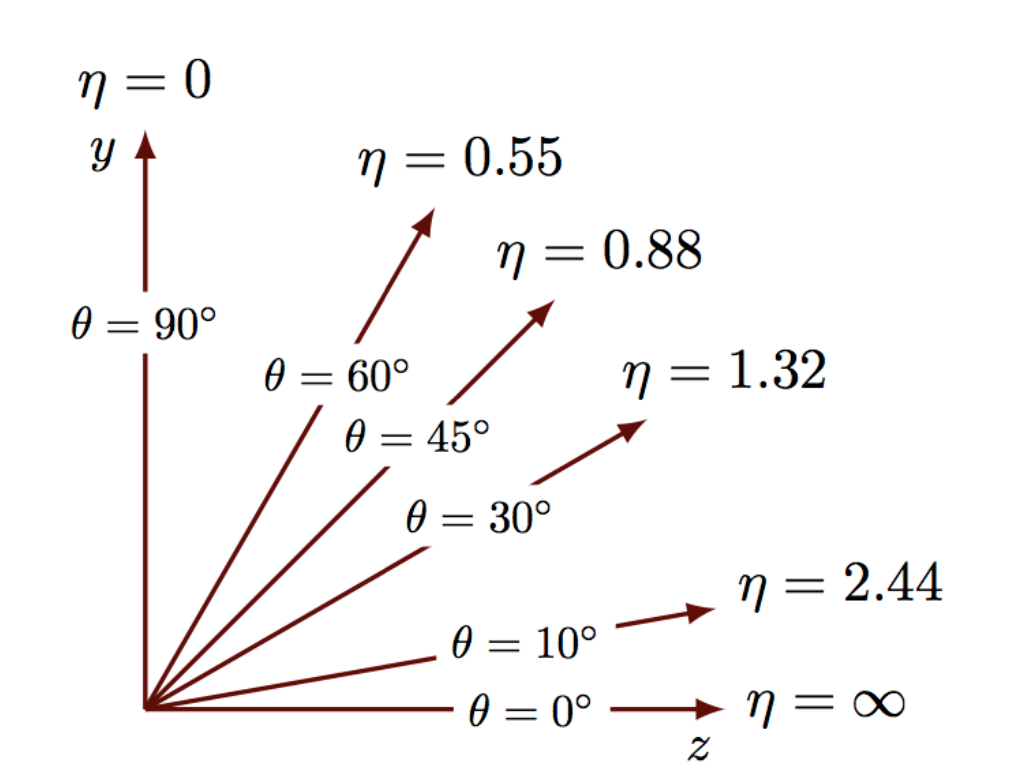
\includegraphics[angle=0,width=0.50\textwidth]{fig/pseudorapidity.png}
\end{center}
\caption{The relationship between $\eta$ and $\theta$.
}
\label{fig:etatheta}
\end{figure}


From the interaction point, collision products traverse layers of materials that are designed to identify, and absorb the energy of most of the particles. These layers are assembled in the following order: 1.) Tracker System, 2.) Electromagnetic Calorimeter, 3.) Hadron Calorimeter, 4.) Muon System. The particles first traverse the Silicon Tracker system which records the position or ``hits" of charged particles. 


The CMS silicon tracker system, records particle paths accurately but are of lightweight material such that they disturb the particle trajectory as little as possible~\cite{CMS:2008xjf}. In addition, they tolerate high radiation fluxes since they are close to the interaction point. Combining the information collected one could reconstruct charged particle $p_T$, and the particles could be traced back to a specific vertex. This information is used in pileup mitigation. 

The next two layers of the CMS detector are the calorimeters that measure the energies of electromagnetic and hadronic particles. Particles going through matter produce a shower, where each interaction with atomic nuclei produces secondary particles, which goes into a repetitive process of cascading particles until the full energy of the initial particle is spent. Ideally, full shower should be captured by the calorimeter so that a more accurate energy value could be reconstructed. We discuss them in more detail in the next two subsections.

Finally, the Muon system characterizes the muons which are minimally ionizing and can escape the calorimeters due to their long life-times and low-energy deposition characteristics. The muons identify muons, measure their momenta, and provide signals for triggering on them via four complementary systems arranged in the steel flux-return yoke of the CMS solenoid. These systems cover a large range of pseudorapidity. The location of the magnetized steel behind the calorimeters and solenoid ensures a low probability of penetration by non-muon or non-neutrino candidates. 

The drift tube system (DT) in the barrel covering $|\eta| < 1.2$ has the task of providing precise spatial measurements and trigger information through drift chambers with rectangular cells. Next, a cathode strip chamber (CSC) system in the endcap covers the forward region with pseudorapidity $0.9 < |\eta| < 2.4$. It has the same task as the DT but is comprised of a different material because of the higher flux of particles in the endcaps, and it also has a faster response time. Additionally, RPCs or resistive plate chambers -- double-gap chambers operated in avalanche mode are placed in both the barrel and endcap to complement the DTs and RPCs to unambiguously identify the bunch crossing corresponding to a muon trigger candidate. It also has a rapid response time~\cite{CMS:2023gfb}.

\begin{figure}[tbp!]
\begin{center}
% 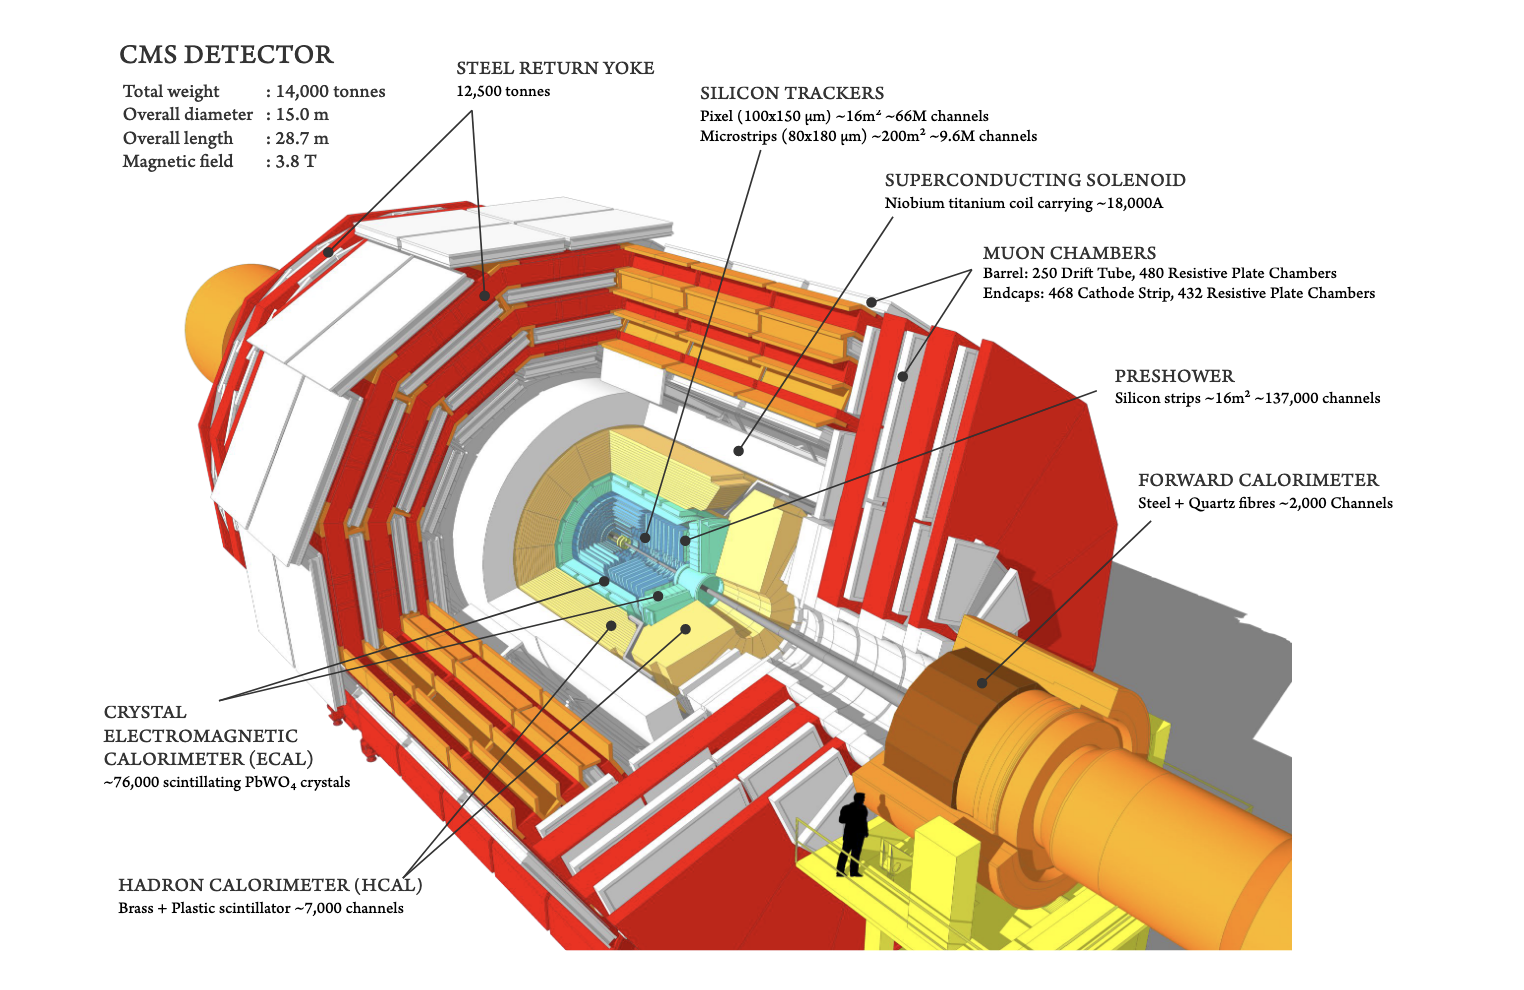
\includegraphics[angle=0,width=0.50\textwidth]{fig/CutawayViewCMSDetector.png}
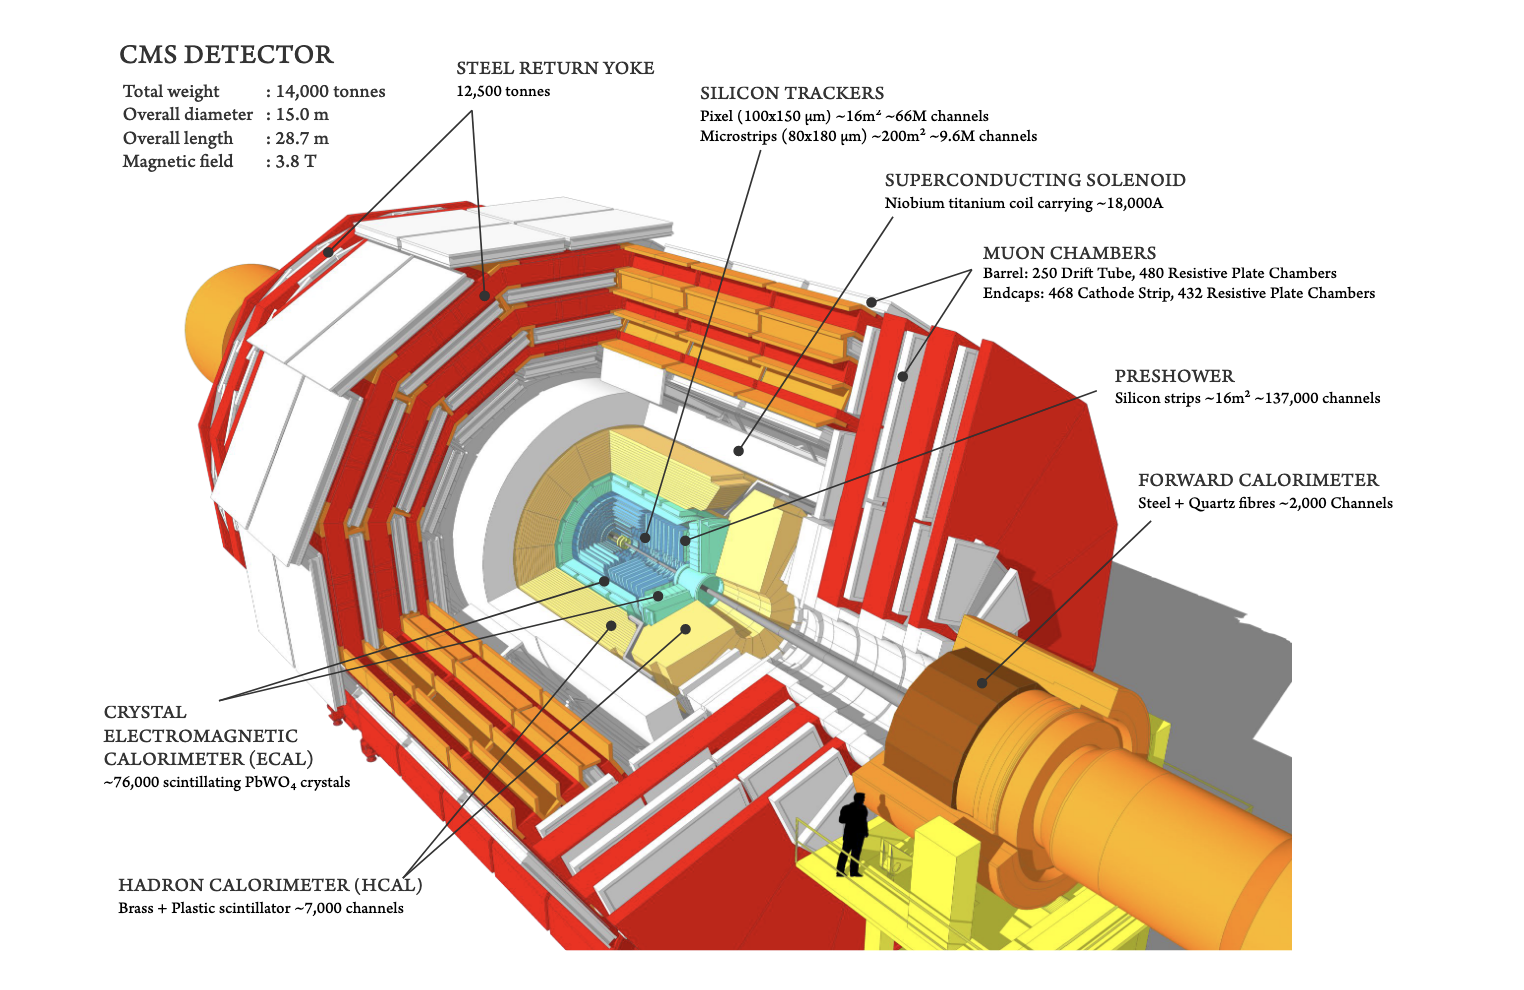
\includegraphics[scale=0.5]{fig/CutawayViewCMSDetector.png}
\end{center}
\caption{A cutaway view of the CMS detector showing its components~\cite{Sakuma:2013jqa}.
}
\label{fig:CMSdetectorCutaway}
\end{figure}

\subsection{ECAL}

The Electromagnetic calorimeter or ECAL, is the second layer of subdetectors that particles go through after the tracker. The ECAL is designed to measure the energies of particles that interact electromagnetically, particularly photons and electrons. It is made of a homogeneous and hermetic lead tungstate (PbW$\text{O}_4$) crystal calorimeter. Homogeneous calorimeters act both as absorbers and scintillators.
As the incident particle interacts with the atomic nuclei of the crystal, electromagnetic showers are induced. Ionization is induced in the atoms and light is emitted as they de-excite. In short, the scintillators convert energy from the showers to light that is in proportion to the incident particle's energy.

There are about 75000 lead tungstate crystals, 61200 of those are spread across the barrel section (EB), located 1.29 meters from the beam line, and the rest are placed at the circular endcaps (EE) which are at $\pm 3.14$ m from the detector origin. Each endcap seals the barrel, with 7324 crystals which gives coverage up to $|\eta| < 3.0$. The EB covers a pseudorapidity range of $|\eta| < 1.479$ where the crystals are laid out in a $170\times360$ $\eta$-$\phi$ grid. In the EE, the crystals are placed in an x-y grid, with a pseudorapidity coverage of $1.479 <|\eta| < 2.5$. 

There are dimensional differences in the EB and EE crystals. The EB crystals have dimensions of about $22\times22$ mm$^2$ in the front-and-rear-facing sides and are 230 mm is in length, corresponding to 25.8 radiation lengths $X_{0}$. The radiation length of a material is the mean length for an electron to lose all but $1/e$ of its original energy. The EB gives a $\Delta \eta$-$\Delta \phi = 0.174\times0.0174$ granularity. To prevent particles from slipping through the spaces in between, the crystals are tilted at 3$^{\circ}$ with respect to the interaction point normal. The endcap crystals have dimensions of $28.6\times28.6$ mm$^2$ in x-y and has a length of 220 mm which corresponds to 24.7$X_0$. 

To facilitate assembly of the detector, the crystals are arranged into groups supermodules in the EB and supercrystals in the EE. There are 36 identical supermodules in the EB and each of these covering half of the barrel length. The supermodules are made up of 4 modules that containe 2 rows of 5 crystals. In the EE, the supercrystals are $5\times5$ structures of crystals, where the inter-crystal gaps are 320 $\mu m$. Each supercrystals have a gap of $2$ mm between them.

Additionally, a preshower detector (ES) is placed in front of the EE with a pseudorapidity coverage of $1.653 < |\eta| < 2.6$ . These are used to help distinguish between photons and $\pi_{0}$ decays which mimic a single photon signature. The ES is a sampling calorimeter made of 2 disks of lead absorbers and 2 planes of silicon strip detectors which act mainly as scintillators. These provide about 3$X_{0}$ of material which impacts the energy resolution in the EE relative to EB. 

The energy resolution as a function of the energy E is as follows:

The energy resolution of the ECAL as a function of energy $E$ is characterized by separate terms added in quadrature of the form
\begin{equation}\label{eq:ECALEnergyRes}
	\frac{\sigma_E}{E} = \frac{a}{\sqrt{E}}\,\oplus\,\frac{b}{E}\,\oplus\,c
 \label{eq:energyresolution}
\end{equation}

% \begin{equation}
%     \frac{\sigma}{E} = \frac{a}{\sqrt{E}} \bigoplus  \frac{b}{E} \bigoplus c
%     \label{energyresolution}
% \end{equation}
where $a$ is a stochastic term related to the statistical nature of shower containment, $b$ is a noise term accounting for electronic terms, and c is a constant term dependent on the intercalibration of the readout channels. These terms are measured in test beam studies to be a = 2.8 $\%$, b = 12 $\%$, and c = 0.3$\%$. At high energies, the constant term dominates but is corrected for by the laser monitoring system. 

To amplify the light yield from the crystals, solid-state avalanche photodiodes (APDs) and vacuum phototriodes (VPTs) are fitted to the rear ends of the EB and EE crystals respectively. VPTs, a type of photomultiplier are chosen for the EE since magnetic field lines are bent there and higher radiation levels are present. There are two APDs that serve each crystal and each are operated at a gain of around 50. The VPTs are also operated at a gain of around 50 but require significantly higher bias voltages. From these photodetectors, the signals are passed off to the detector electronics for processing. These are discussed further in the Trigger and Electronics subsection. 

\begin{figure}[tbp!]
\begin{center}
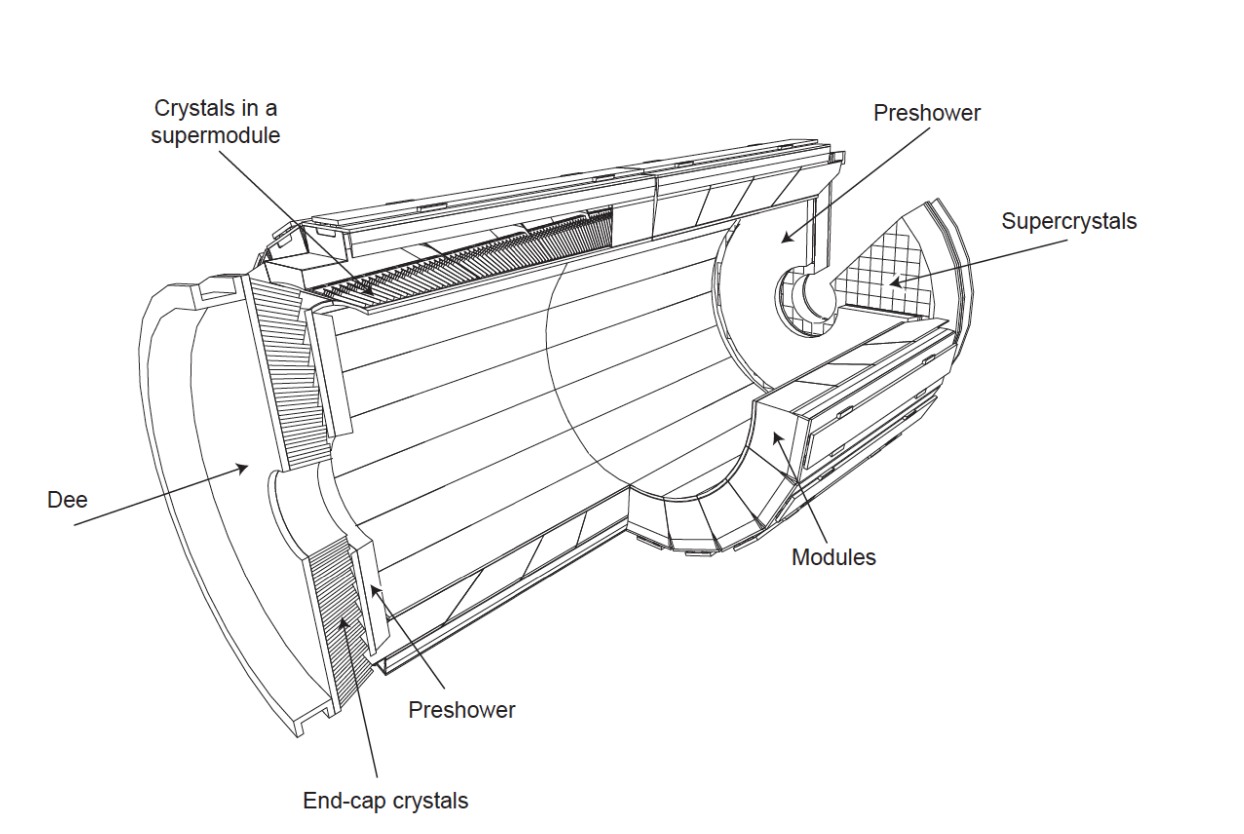
\includegraphics[scale=0.7]{fig/cutawayECAL.png}H
\end{center}
\caption{A cutaway view of the ECAL and its components~\cite{Chatrchyan:2008aa}.
}
\label{fig:cutawayECAL}
\end{figure}


\subsection{HCAL}

The Hadronic Calorimeter (HCAL) is designed to measure the energy of hadrons that are typically contained in jets. Hadronic showers are more complicated than electromagnetic showers, i.e. the cascade of different particles coming from strong interactions with the nuclei contain charged or neutral pions or neutrinos. This fact poses challenges with the energy resolution and providing coverage for missing energy. For these reasons, the HCAL is substantially longer than the ECAL to fully contain the energy of the incident hadrons. 

Due to budgetary and material constraints, the HCAL cannot be made with the same homogeneous calorimeter material like the ECAL is made from. Instead, it is built as a sampling calorimeter with alternating layers of steel and brass absorber plates and plastic scintillator tiles for most sections of the HCAL. The scintillator tiles carries light through wavelength-shifting fibers to photodetectors that convert the light pulses to electric signals. The sum of the light across the entire shower is proportional to the total energy of the incident hadrons. 

The HCAL is comprised of four subdetectors: The HCAL Barrel (HB) the HCAL Endcaps (HE), the HCAL Forward (HF) and the HCAL Outer (HO). The first two cover up to $|\eta| < 3$. Beyond the HE region, a complementary Cherenkov-light-based system called the HF (Forward), extends the coverage up to $|\eta| <5$. Outside of the magnet, the HO system, with coverage of $|\eta| < 1.26$ has additional scintillators that are installed to complement and improve the energy resolution in the HB. 

\begin{figure}[tbp!]
\begin{center}
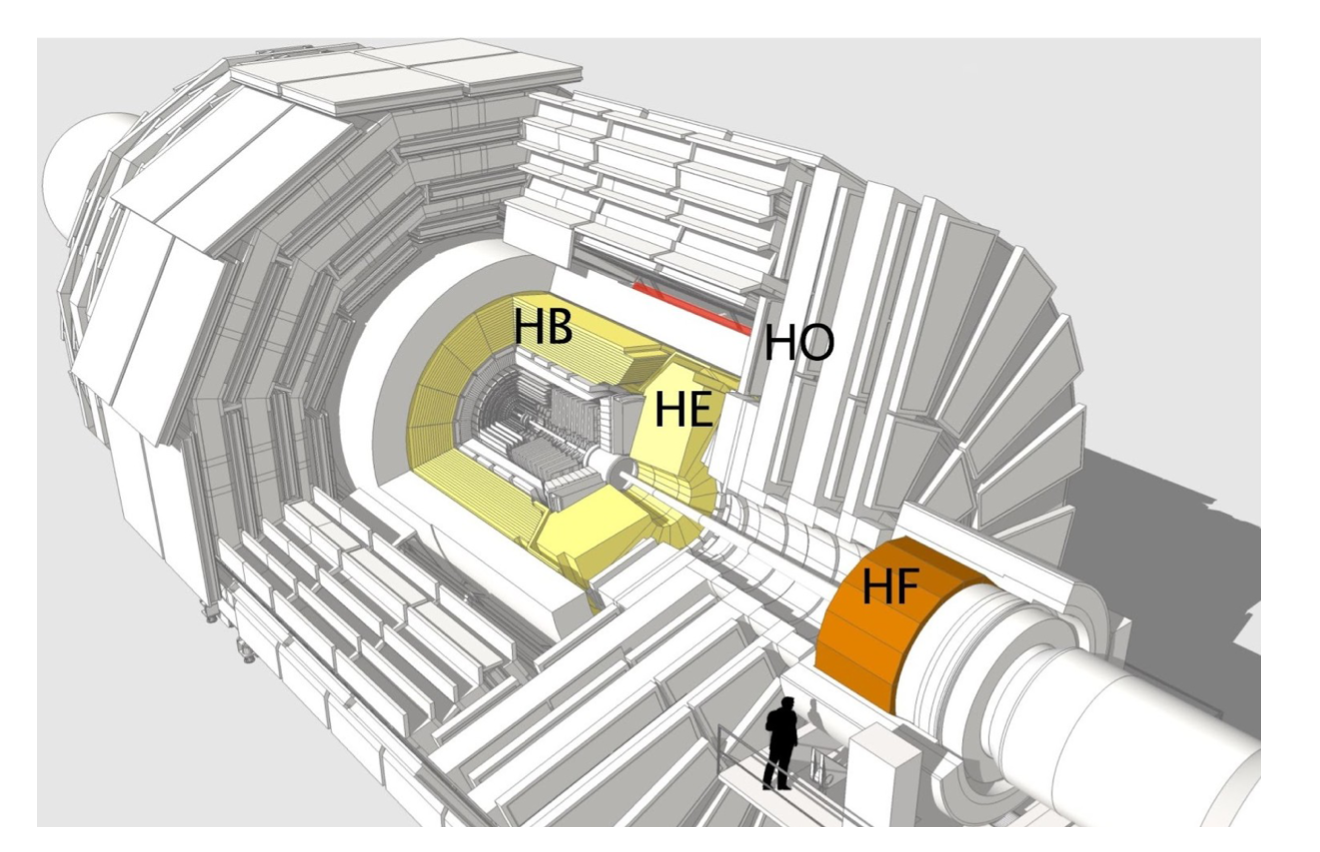
\includegraphics[scale=0.6]{fig/LabelledHCAL.png}
\end{center}
\caption{A cutaway view of the HCAL and its subdetectors~\cite{Chatrchyan:2008aa}
}
\label{fig:HCAL}
\end{figure}


% \begin{figure}[!htb]
% 	\centering
% 	\includegraphics[scale=0.65]{figures/hcal}
% 	\caption{A projection of the HCAL, highlighting its subdetectors~\cite{Chatrchyan:2008aa}.}
% 	\label{hcal}
% \end{figure}

The barrel region of the HCAL consists of the HCAL Barrel (HB) and the HCAL Outer (HO). The HB is situated between the CMS solenoid magnet and the ECAL and spans a radial distance of $1.77 < r < 2.96$ m, with a pseudorapidity coverage $|\eta| < 1.3$. The first layer of the HCAL consists of a plastic scintillator made of 9 mm Bicron BC408 which is different from the succeeding layers of scintillators. This upgrade was made to enhance the depth-segmented readout~\cite{Cummings_phdThesis}} which was made to measure the hadronic showers that began in the ECAL. The information obtained from this layer directly affects our photon identification strategy. The first and last layers of are made of stainless steel absorbers for the purposes of structural support. In between are pairs of brass absorber plates and plastic scintillators. Brass was chosen for cost-effectiveness and robustness against deformation under the strong 4T solenoid field. While these material provide excellent shower containment, the HO was placed behind the solenoid magnet to provide additional detection for the shower tails extending beyond HB. It is made of 10 mm the same scintillator material found behind the ECAL and an additional layer of iron absorber. The HB+HO combination provide an effective thickness of 11.8 nuclear interaction lengths $\lambda_{I}$. Nuclear interaction length is defined as the mean distance travelleld by a hadronic particle before undergoing an inelastic nuclear interaction.

The HCAL endcaps are located between $ 3.9 < |z| < 5.7$ and covers the range $1.3 < |\eta| < 3.0$. As mentioned earlier, the HF extends coverage in the forward region to $|\eta| = 5.2$, located 11.2 m from the detector origin. Instead of plastic scintillators, it uses quartz fibers as the active material to produce Cherenkov light. The forward region experiences the highest particle fluxes in the detector, about 8 times as much as other subdetectors and therefore the switch in material. Steel absorbers are used in the HF. 

The HB+HE region provides a granularity of $\Delta \eta \times \Delta \phi= 0.087 \times 0.087$, a similar coverage of $5\times5$ EB crystals for $|\eta| < 1.6$ while for $|\eta| > 1.6$ the granularity is coarser $\Delta \eta \times \Delta \phi= 0.174 \times 0.174$. Across the depth of a single $\Delta \eta$ region, towers of scintillation light are formed. The plastic scintillators of the towers are connected to wavelength-shifting (WLS) fibres which are routed to hybrid photodiodes (HPD) which are then read out to the electronics for processing. We discuss more on the electronics in later sections.  

In terms of resolution, the HCAL performance is much better evaluated with the jet and $p_T$ resolutions of the ECAL + HCAL system instead of just HCAL alone. The results are similar to that described in Eq.~\ref{eq:energyresolution}.

\subsection{CMS Data Trigger and Electronics }

The LHC proton-proton collisions occur every 25 ns, or 40 MHz. This corresponds to a 1 MB average event size, with 40 PB of data if every event was to be recorded. In one year alone, the data produced by the LHC is around one order of magnitude bigger than the total size of objects ever stored on commercial cloud storage services making the LHC one of the most prominent players in the Big Data era~\cite{Clissa:2021}. The strategy then is to determine in advance only the events that are of interest. CMS does this with a two-level filtering scheme employed to progressively reduce the data collected. The first stage of event rate reduction, called Level 1 (L1) trigger, is performed by high-speed electronics and uses coarser-grained detector information. The event rate is reduced from 40 MHz to about 100 kHz. In the second stage, the high-level trigger (HLT), is software-based menus to further reduce the rate even further from 100 kHz to 2kHz. Unlike L1, HLT uses the full detector granularity, i.e. the information from all the subdetectors including the inner tracks. Only events that pass through both the L1 and HLT are stored for offline physics analysis. Figure~\ref{fig:LHC_BigData} shows how untriggered LHC data compares other Big Data players. 

% \footnote{Overall, high-energy physics events of interest have $p_{T} > 10$ GeV. }

\begin{figure}[tbp!]
\begin{center}
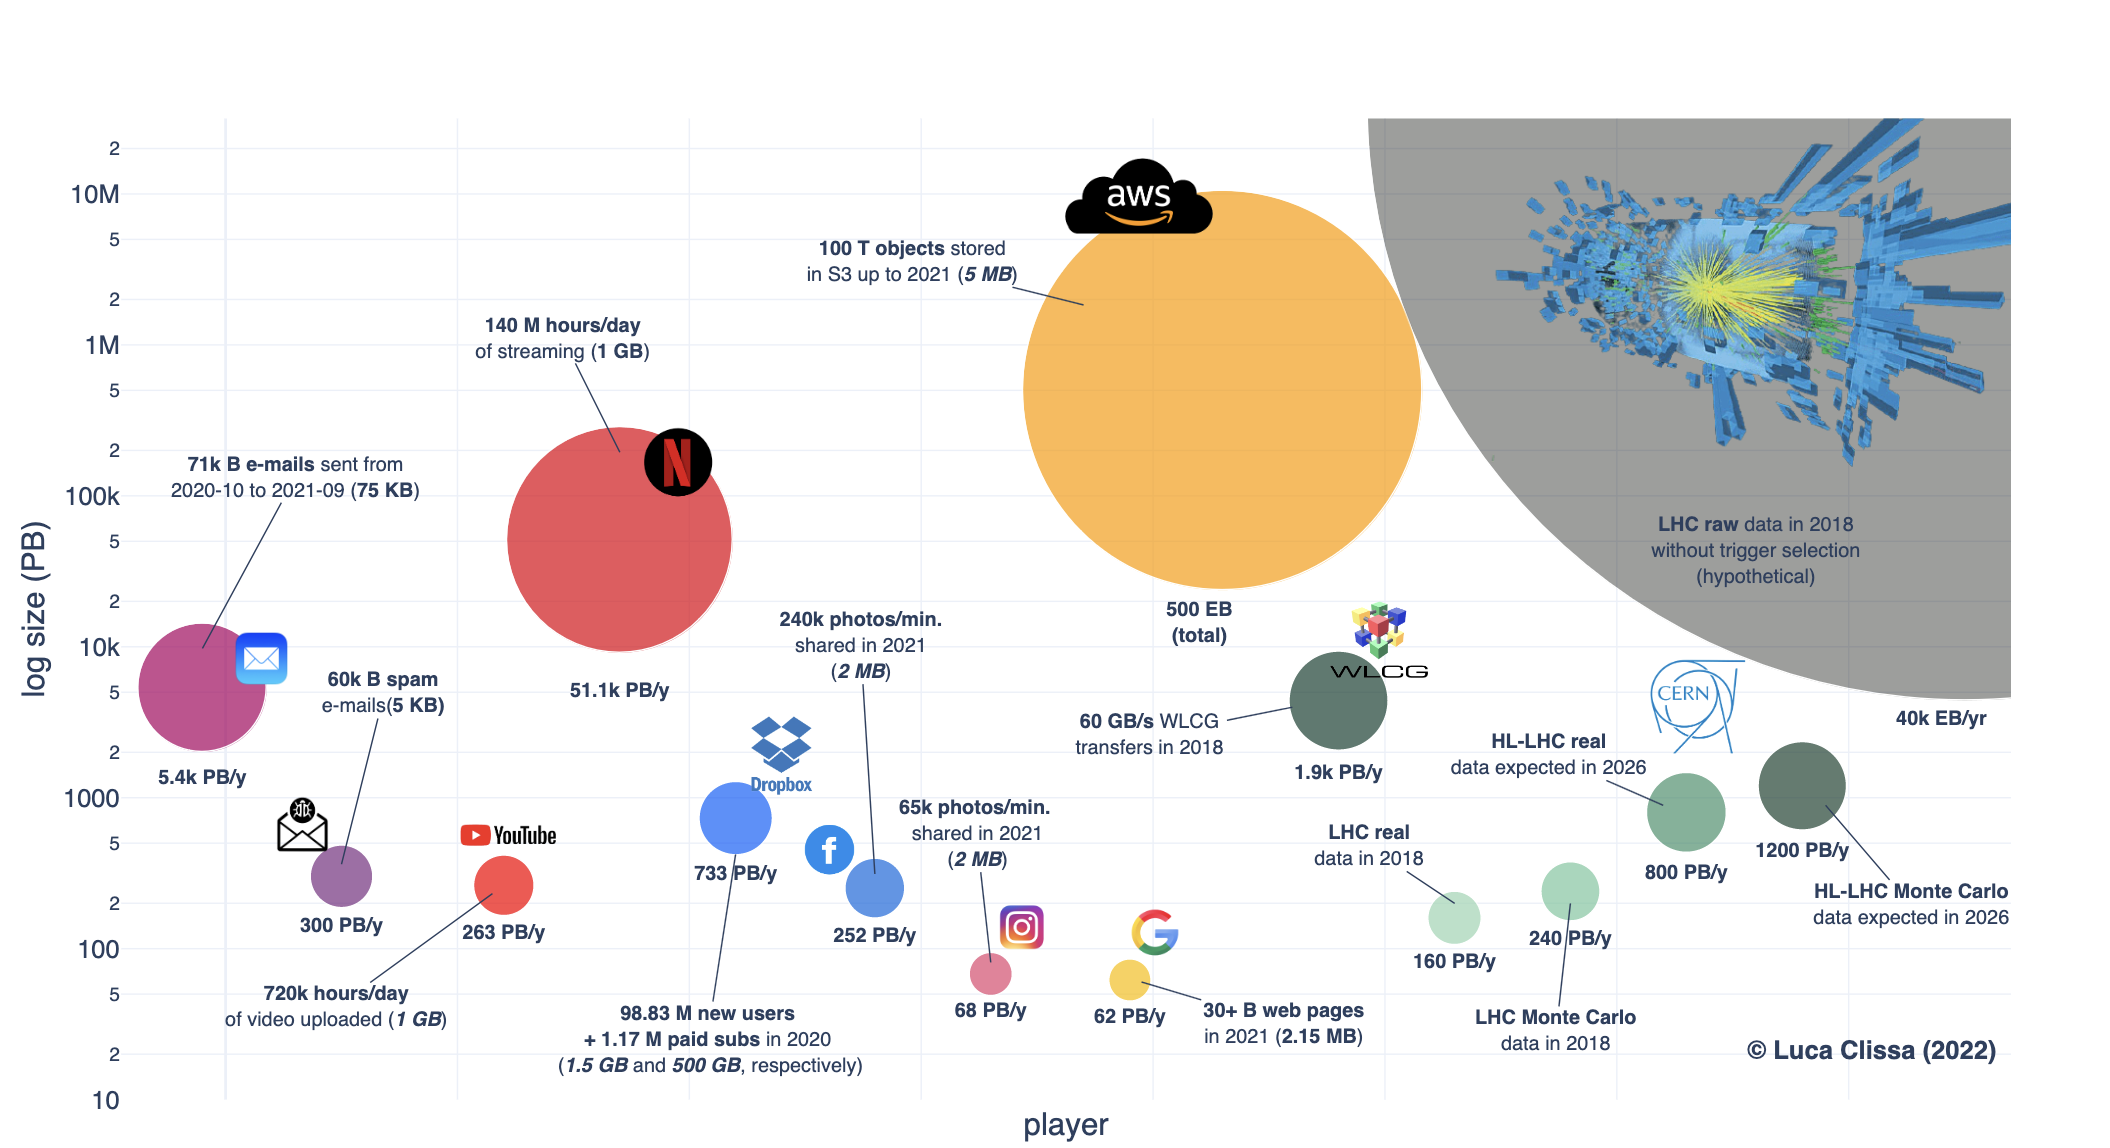
\includegraphics[scale=0.4]{fig/BigData.png}
\end{center}
\caption{An illustration comparing the LHC-produced data without trigger selection to the other Big data players~\cite{Clissa:2021}.
}
\label{fig:LHC_BigData}
\end{figure}


\subsubsection{L1 Trigger}
The L1 Trigger system makes a decision to accept an event within 3.2 $\mu s$, with every single step in the decision-making chain made before the next proton-proton bunch crossing, i.e. within less than 25 ns. This speed of decision-making requires custom-programmed FPGAs or ASICs that are situated in the front-end or what is called on-detector electronics. These hardware are characterized for their radiation tolerance being situated so close to the detector components. 

\begin{figure}[tbp!]
\begin{center}
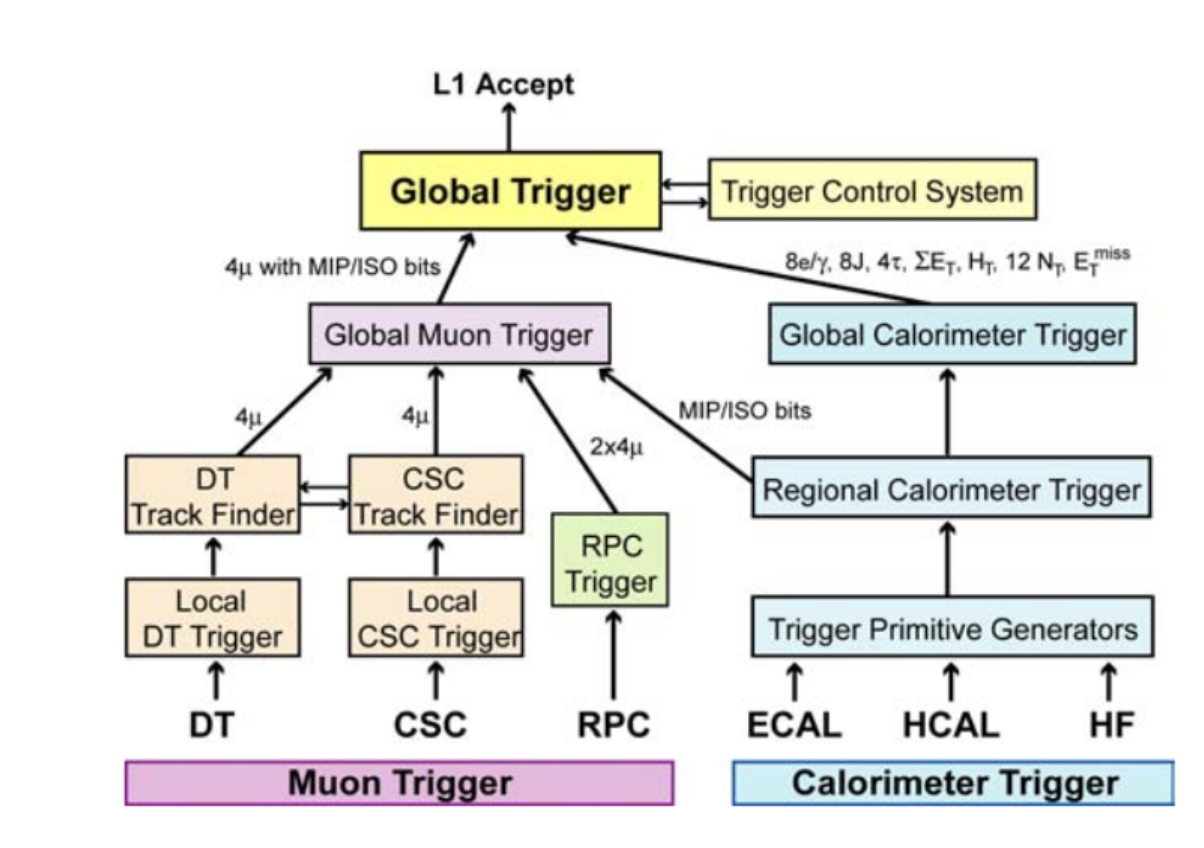
\includegraphics[scale=0.6]{fig/L1Trigger.png}
\end{center}
\caption{A cutaway view of the HCAL and its subdetectors \cite{CMS:2008xjf}
}
\label{fig:L1Trigger}
\end{figure}

The architecture of the L1 system is shown in Figure~\ref{fig:L1Trigger}. An event is ``L1 Accepted" based on aggregated information from the calorimeter and muon systems, both of which are organized into a hierarchy of local, regional and global components. For the Calorimeter Triggers, the first step are the local triggers also known as Trigger Primitive Generators (TPGs) which collect $E_{T}$ deposits from the ECAL or the HCAL trigger towers that have a granularity of $\Delta \eta \times \Delta \phi= 0.087 \times 0.087$. The local TPGs also correct bunch crossing information. In the next step, the TPGs are passed on to the Regional Calorimeter Trigger (RCT) which sums the TPG trigger towers into RCT towers ($4 \times 4$ TPG trigger towers). At this step, crude electromagnetic particle candidates are formed are formed. Finally, a Global Calorimeter Trigger receives the information from the RCT to construct jet candidates, and missing $E_{T}$ candidates and more complex electromagnetic particle candidates. The Muon Trigger has a similar pipeline at L1 begins with information coming from the DT, and CSC muon trackers which provide track hits. The aggregated information is passed on to the Regional Muon Trigger (RMT) which performs track reconstruction. The RPC Trigger information is able to reconstruct complete tracks without any intermediate steps because of its superior timing information. The CSC, DT, and RPC  Trigger Chain are then collectively passed on to the Global Muon Trigger (GMT). The combined Global Muon Trigger (GMT) and Global Calorimeter Triggers (GCT) are then passed on to the Global Trigger which makes the final decision on whether to trigger on the event and pass it on to the HLT.

Events that make it through the HLT must further pass a software-based list of cuts called an HLT menus, to reduce the event rate to 1 kHz. An on-site commercial processing farm of more than 10,000 cores, performs the event reconstruction. In this case, there is more time flexibility with triggering using the full detector granularity. Events that make it through this final step are then recorded for physics analysis. 

The HLT menus consists of a set of simple cuts on single objects or events based on topology. For example, in this analysis, we are interested in events with a two-photon final state. The algorithms used by the HLT are similar to that of the offline Physics Reconstruction which we will discuss in the next chapter. 

\subsection{HCAL Online Software and HCAL Upgrades}

A series of upgrades have been planned for CMS with an eye to prepare the detector for the challenges of the High-Luminosity (HL-LHC) era. The first of the of the series termed Phase 1, in between Run 2 and Run 3, in a period called Long Shutdown (2). In this section we discuss the HCAL Phase I upgrade which was completed in October 2019 in time for Run 3 which was unfortunately pushed later to 2022 due to the COVID-19 pandemic. My contributions to HCAL encompassed upgrades in both HCAL Online Software and both Front-End (FE) and Back-End (BE) Electronics. My major contribution on the HCAL Online Software was work on providing software support for the improved timing information to create an L1 trigger on Long-Lived Particles (LLP), under the supervision of Seth Cooper and Aleko Khukhunaishvilli. I also participated in the refurbishing and accounting of Front-End (FE) and Back-end (BE) electronics which was performed with the team consisting primarily of Grace Cummings, Mary Hadley, Sebastian Yan, Candan Isik and Jay Dittman.

In the first two parts, we first give an overview of the FE and BE electronics in Section~\ref{sec:FEBEHCALElectronics} to guide the reader into the idea behind the L1 trigger on Long-Lived Particles (LLP).

\subsubsection{Front-End and Back-End Electronics}~\label{sec:FEBEHCALElectronics}
The Front-End and Back-End electronics data flow diagram is shown in Figure~\ref{fig:DataFlowHCAL}. The Front-End electronics are composed of units called read-out boxes (RBXs) that contain the following: 4 read out modules or (RMs), 1 calibration unit (CU), Clock, Control and Monitoring Modules (CCMs) and a backplane that connects all the components within an RBX. Each of the RMs cover about a 5 degree division in $\phi$. Each RM is a card pack that has the QIE or charge integration boards and light detectors. The RMs combine light into readout towers and converted into digital data and are transmitted to the back-end electronics. Figure~\ref{fig:ReadOutModules} shows a schematic of the RBXs and Figure~\ref{fig:RBXBurnin904} shows an example RBX set-up at the HCAL test facility at Building 904.

The HCAL Back-end electronics are responsible for receiving the continuous readout information coming from the front-end electronics, calculating and transmitting trigger information, storing and sending the front-end trigger data when a L1-accept has been received from the CMS global trigger~\cite{Cooper:2016kef}. Figure~\ref{fig:DataFlowHCAL} shows a schematic diagram for the backend. It also has a local data acquisition and triggering mode, and also handles fast clock and control signals. Back-end crates are called $\mu$TCA crates which contain an Advanced Mezzanine Card (AMC13) which is responsible for event building and linking the back-end to the CMS central data acquisition (cDAQ) system. The $\mu$HTR performs two functions via the two Xilinx FPGAs. The front FPGA takes input from the front-end data, synchronizes the data and pipelines and calculates and transmits the trigger information. The back FPGA is responsible for buffering and applying zero suppression and transmits data to cDAQ. The upgraded electronics include increased granularity and feature bits based on TDC information which will be relevant in our work on the software support for the HB TDC LUTs. 

I was part of the last phase of the ngCCM refurbishing project and I also helped coordinate the start of the front-end and back-end electronic spares bookkeeping and preparation. The refurbishing of the ngCCMs is largely because of a communication issue loss which was attributed to a manufacturing weakness in the VTRxs. The VTRx optical receivers were found to be temperature-sensitive with temperature increases causing outgassing material to obscure the central part of the optical fibers where light is transmitted~\cite{Cummings:2022kgm}. To mitigate the issue, heat sinks were added within the ngCCMs. 

I also began the preparation of the new AMC13s which were production-tested by Chris Cosby from Boston University. I also updated the firmware to match the latest firmware at P5 which was T1, T2 = $0\times2266$ $0\times34$. As there was not a good criteria as to what would qualify as a good spare, I went through several testing steps such as local event building tests and taking local runs with the new AMC13s loaded in the mock up test area of Bldg. 904 at the CERN Prevessin site. We determined that the final step before swapping them at P5~\footnote{Jay Dittman also proposed that we could swap the five spares with the AMC13s that are known to be working well at P5 so we have 'good hot spares'.} was to do a 904 miniDAQ testing. Local runs do not test cDAQ links. As the miniDAQ software was not well configured before my stay at CERN ended, I delegated the tasks to the rest of the team who would take over the project. Figure~\ref{fig:BackendCrate9041} and Figure~\ref{fig:BackendCrate9042} shows the reworking and testing setups for the AMC13 and ngCCM testing. Credits to Jay Dittman and Grace Cummings for the set-up.

In the first half 2021, I have also participated DAQ On-call and DCS Technical shifts at P5 as well as in the updating of the firmwares for the igloo2 FPGAs in the HF ngCCMs located at the CMS cavern shown in Figure~\ref{fig:HFIglooReprogramming}. 

% \begin{figure}[tbp!]
% \label{fig:DataFlowHCAL}
% \begin{center}
% 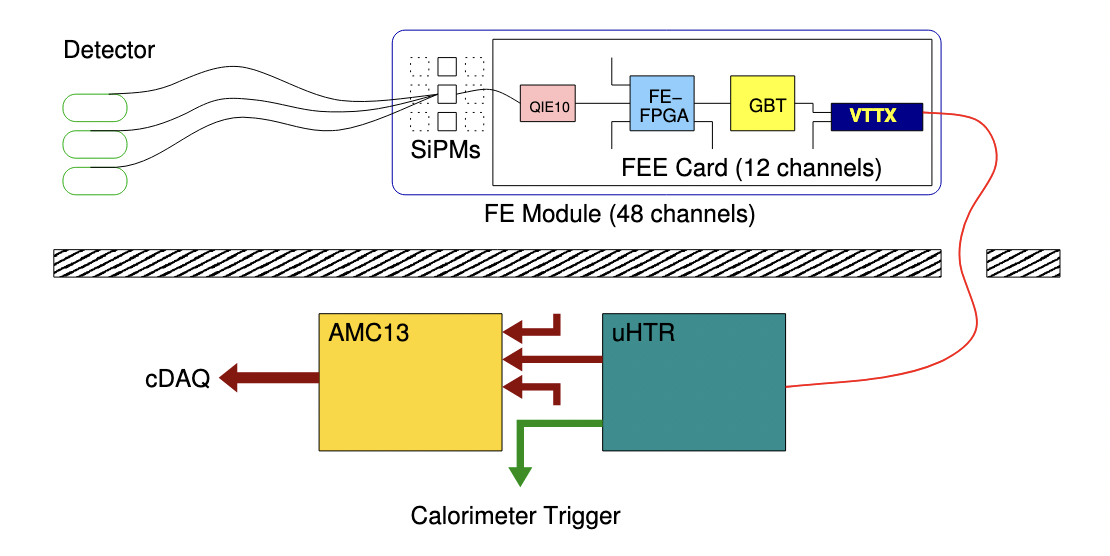
\includegraphics[scale=0.6]{fig/CalorimeterTrigger.png}
% \end{center}
% \caption{ Schematic diagram of the data flow in HB/HE starting from the photomultipliers through the QIE, FPGA and to the backend and AMC13 and to the CMS DAQ~\cite{Cooper:2016kef}.
% }
% \end{figure}

\begin{figure}
\centering
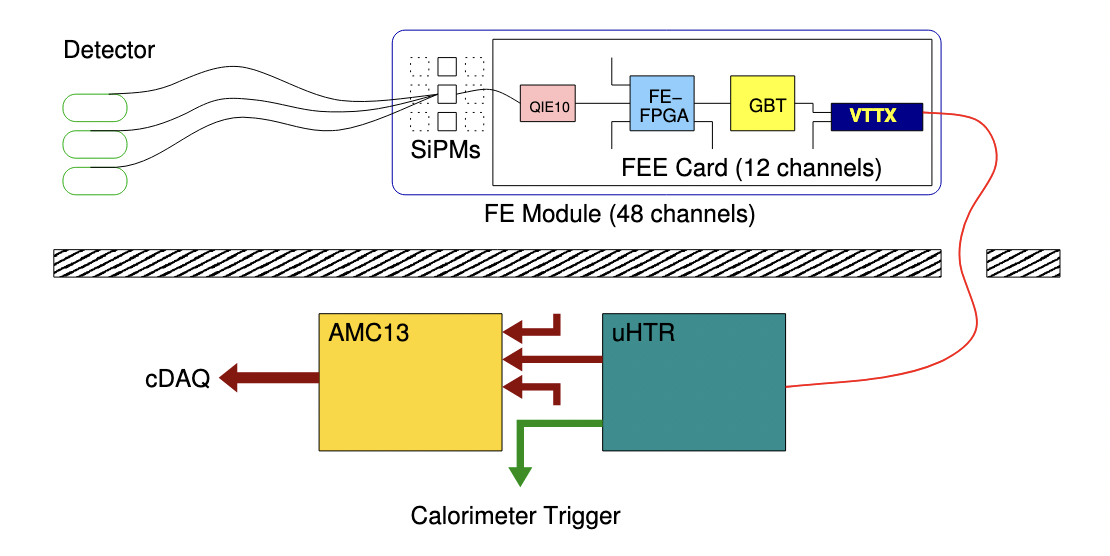
\includegraphics[scale=0.6]{fig/CalorimeterTrigger.png}
\caption{Schematic diagram of the data flow in HB/HE starting from the photomultipliers through the QIE, FPGA and to the backend and AMC13 and to the CMS DAQ~\cite{Cooper:2016kef}.}
\label{fig:DataFlowHCAL}
\end{figure}


\begin{figure}[!htb]
	\centering
	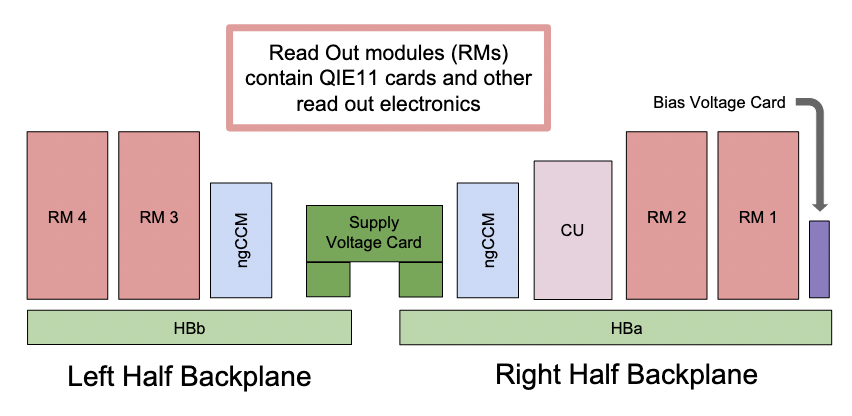
\includegraphics[scale=0.7]{fig/RMs.png}
	\caption{A schematic diagram of an HB RBX containing the 4 RMs, 2 ngCCMs and the backplanes~\cite{Cummings_phdThesis}}
	\label{fig:ReadOutModules}
\end{figure}

\begin{figure}[!htb]
	\centering
	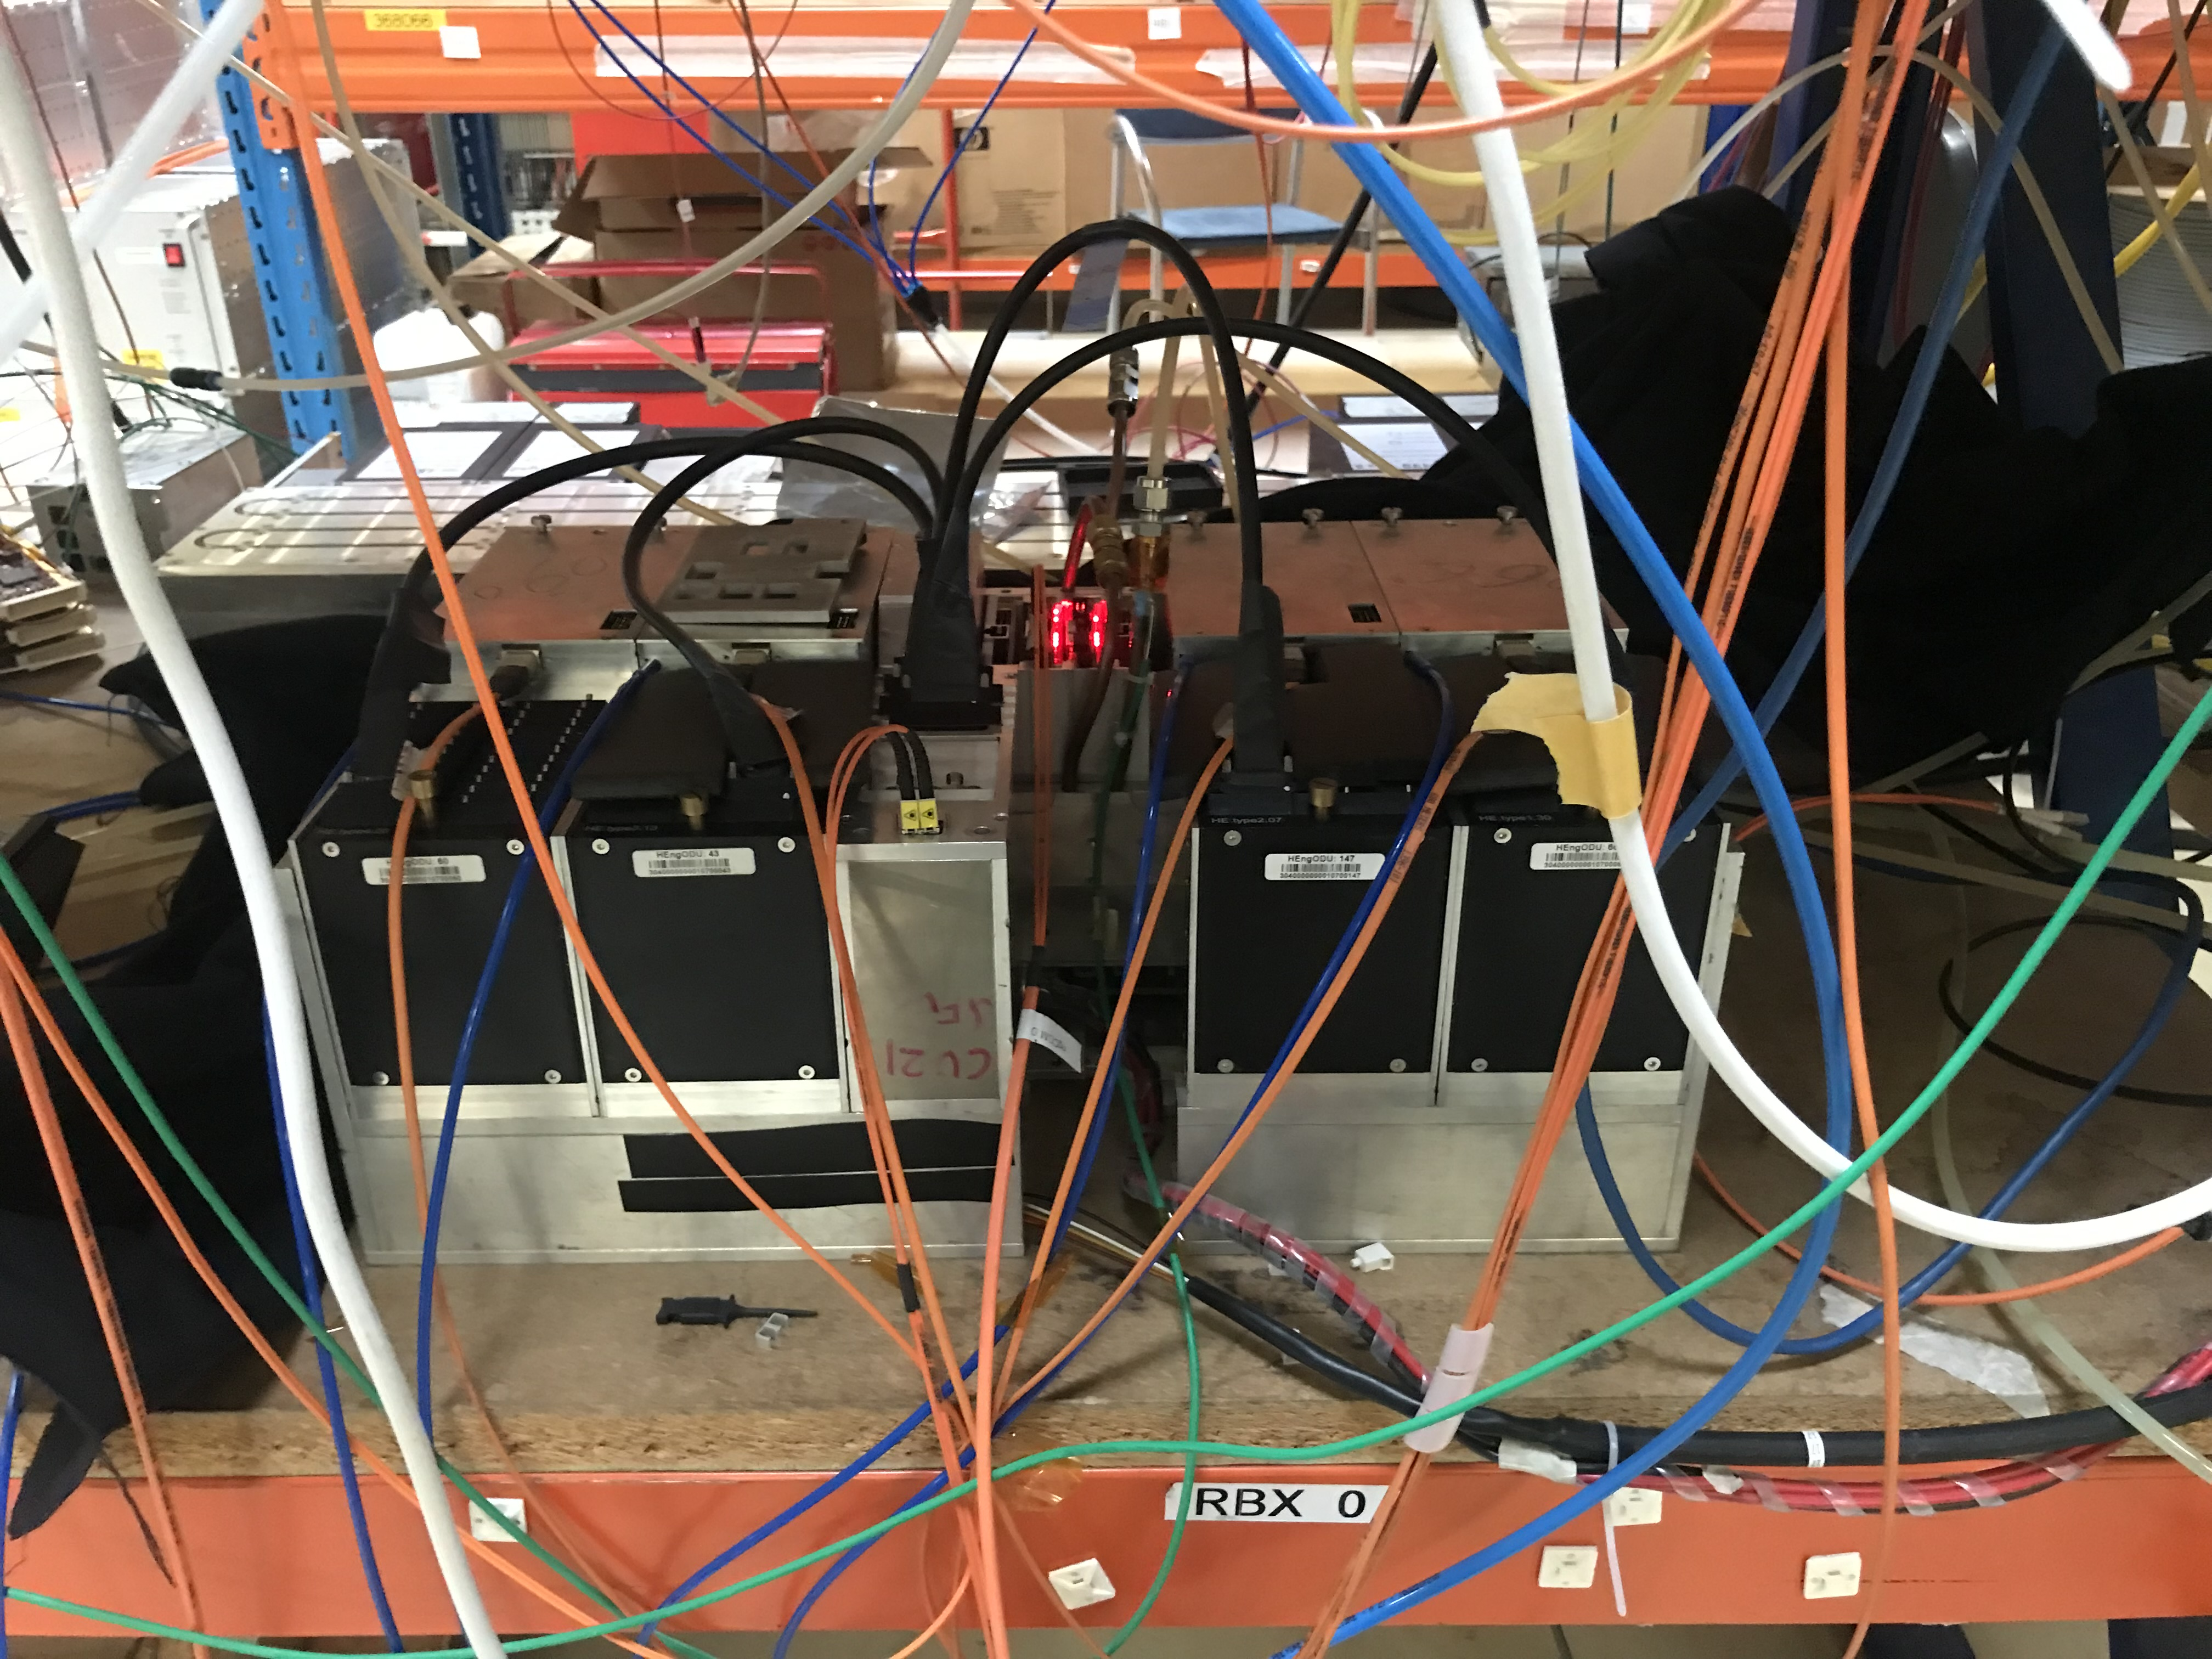
\includegraphics[scale=0.07]{fig/RBXBurn-in.jpg}
	\caption{Image of an RBX at Building 904 where a mock-up of the CMS HCAL Front-End electronics are set up for testing.}
	\label{fig:RBXBurnin904}
\end{figure}

% \begin{figure}[!htb]
% 	\centering
% 	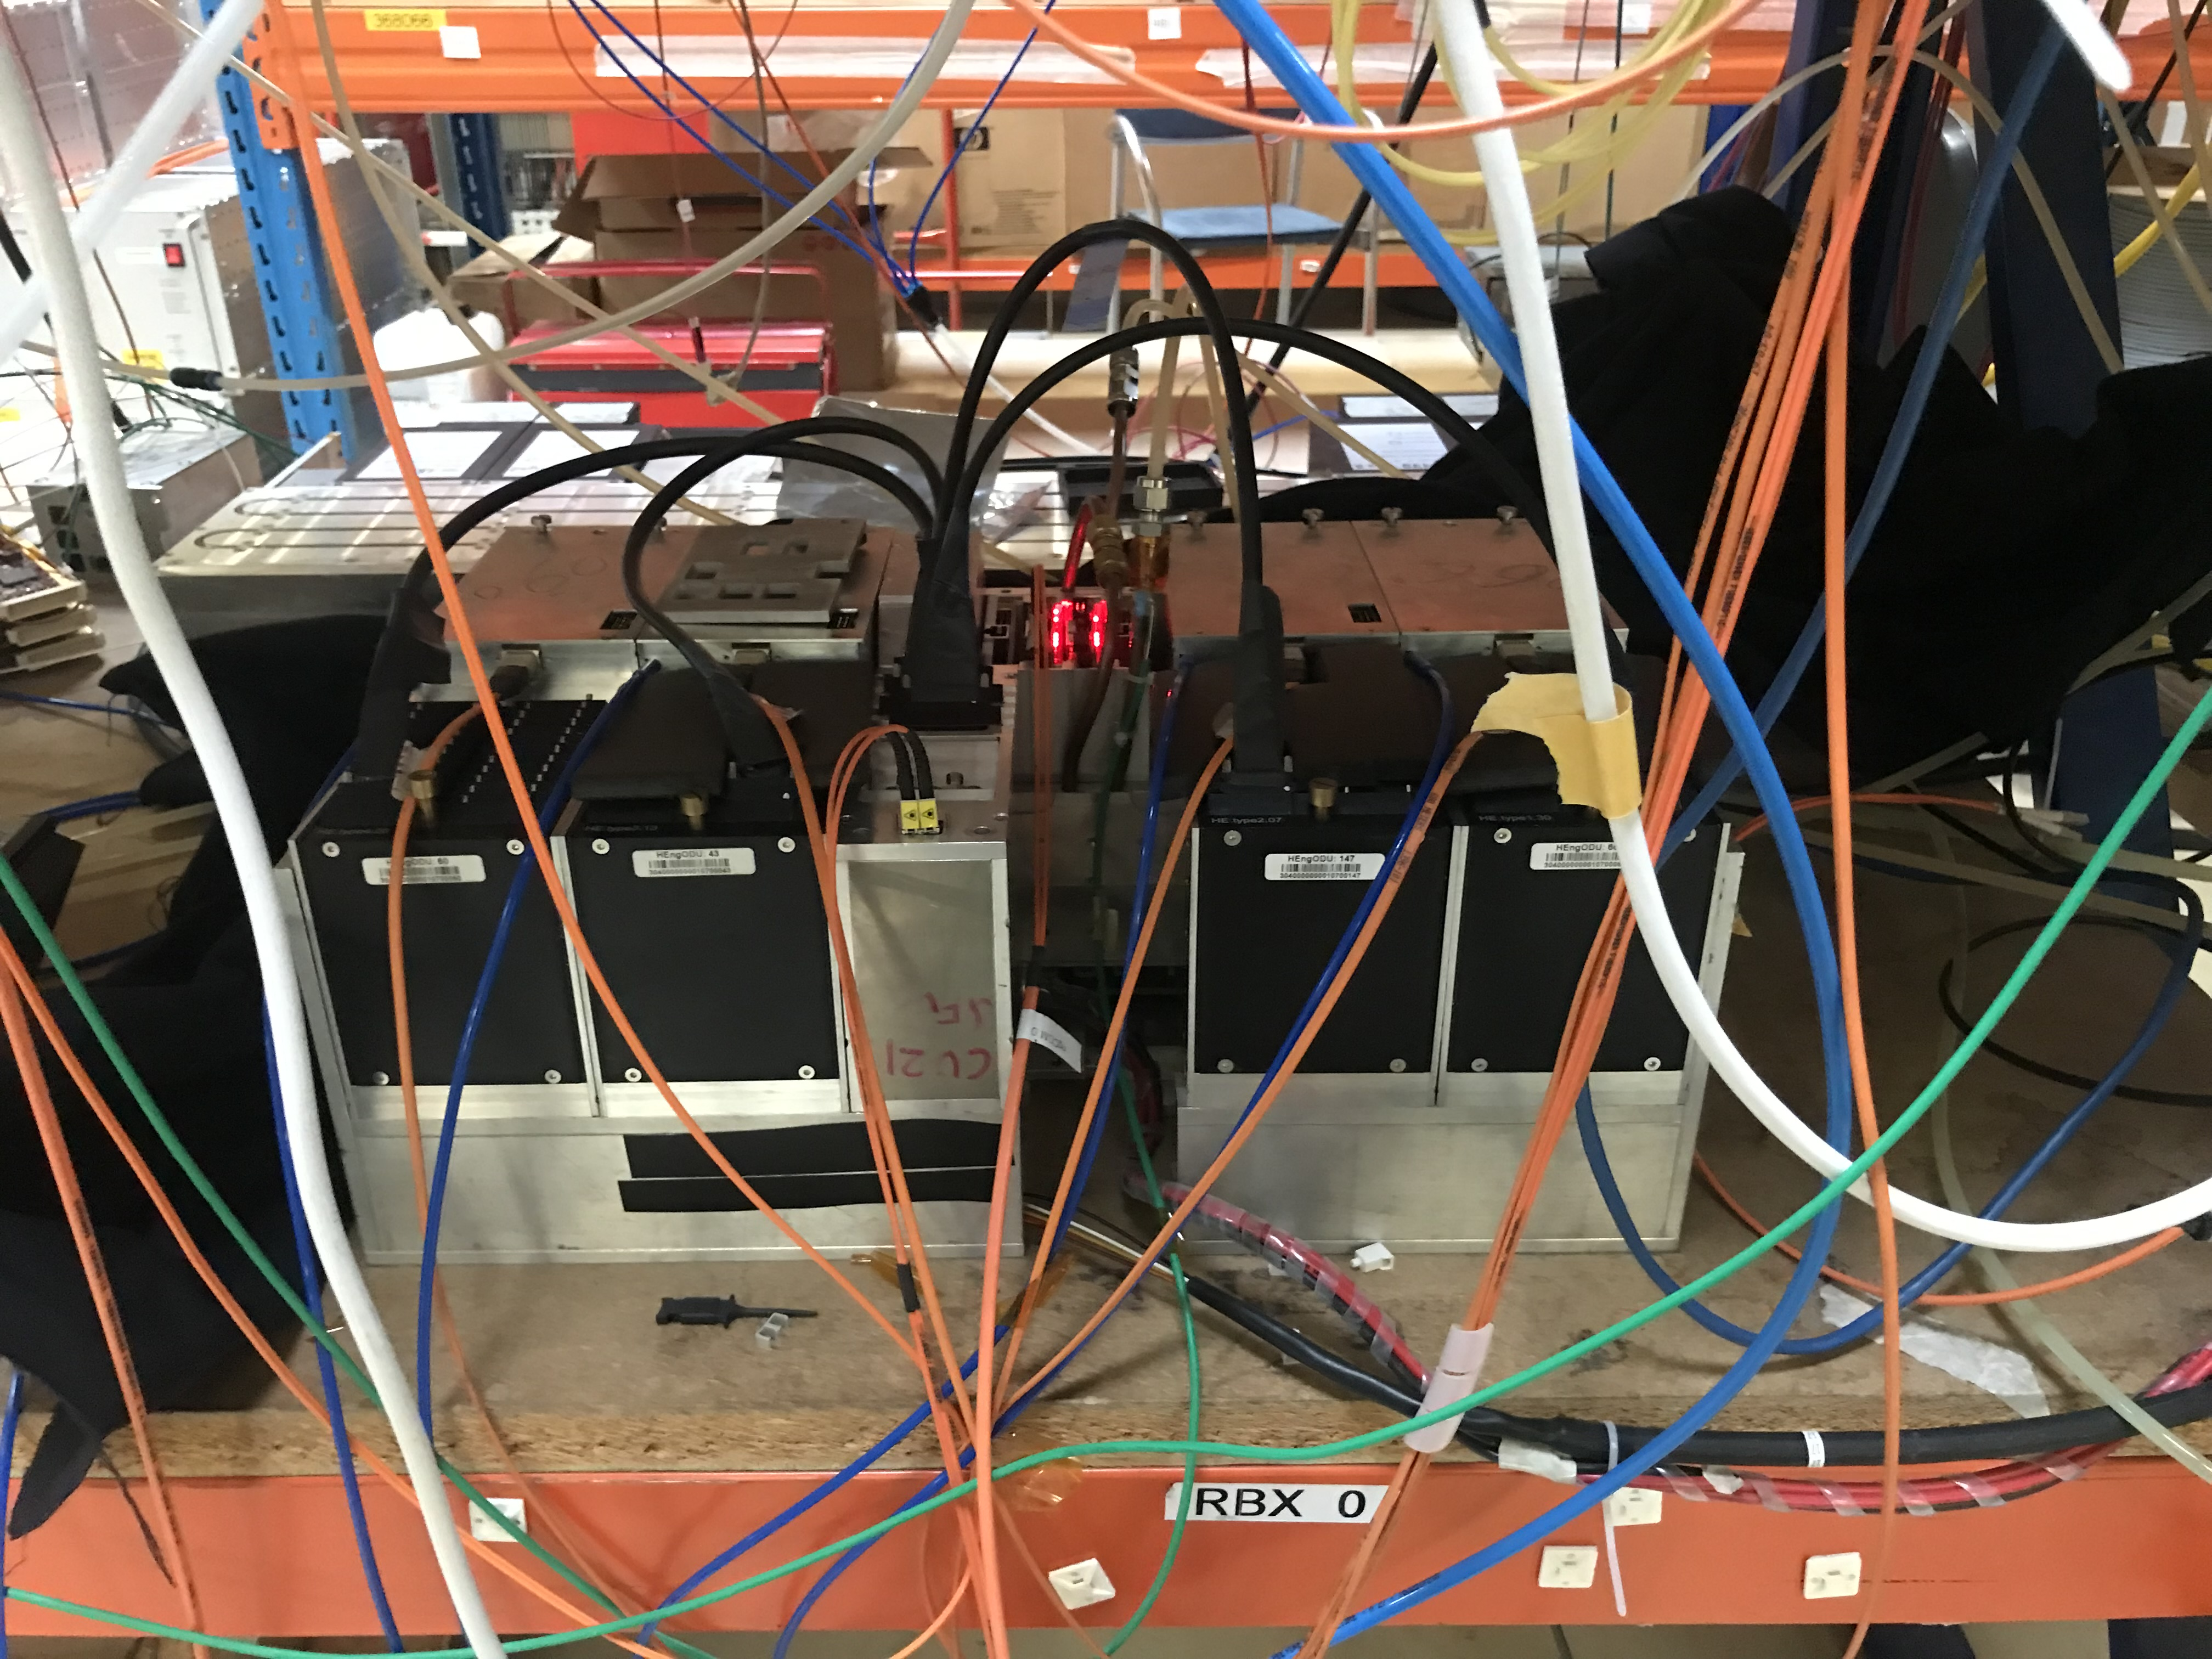
\includegraphics[scale=0.07]{fig/RBXBurn-in.jpg}
% 	\caption{Image of an RBX at Building 904 where a mock-up of the CMS HCAL Front-End electronics are set up for testing.}
% 	\label{fig:BackendCrate904}
% \end{figure}

\begin{figure}[!htb]
	\centering
	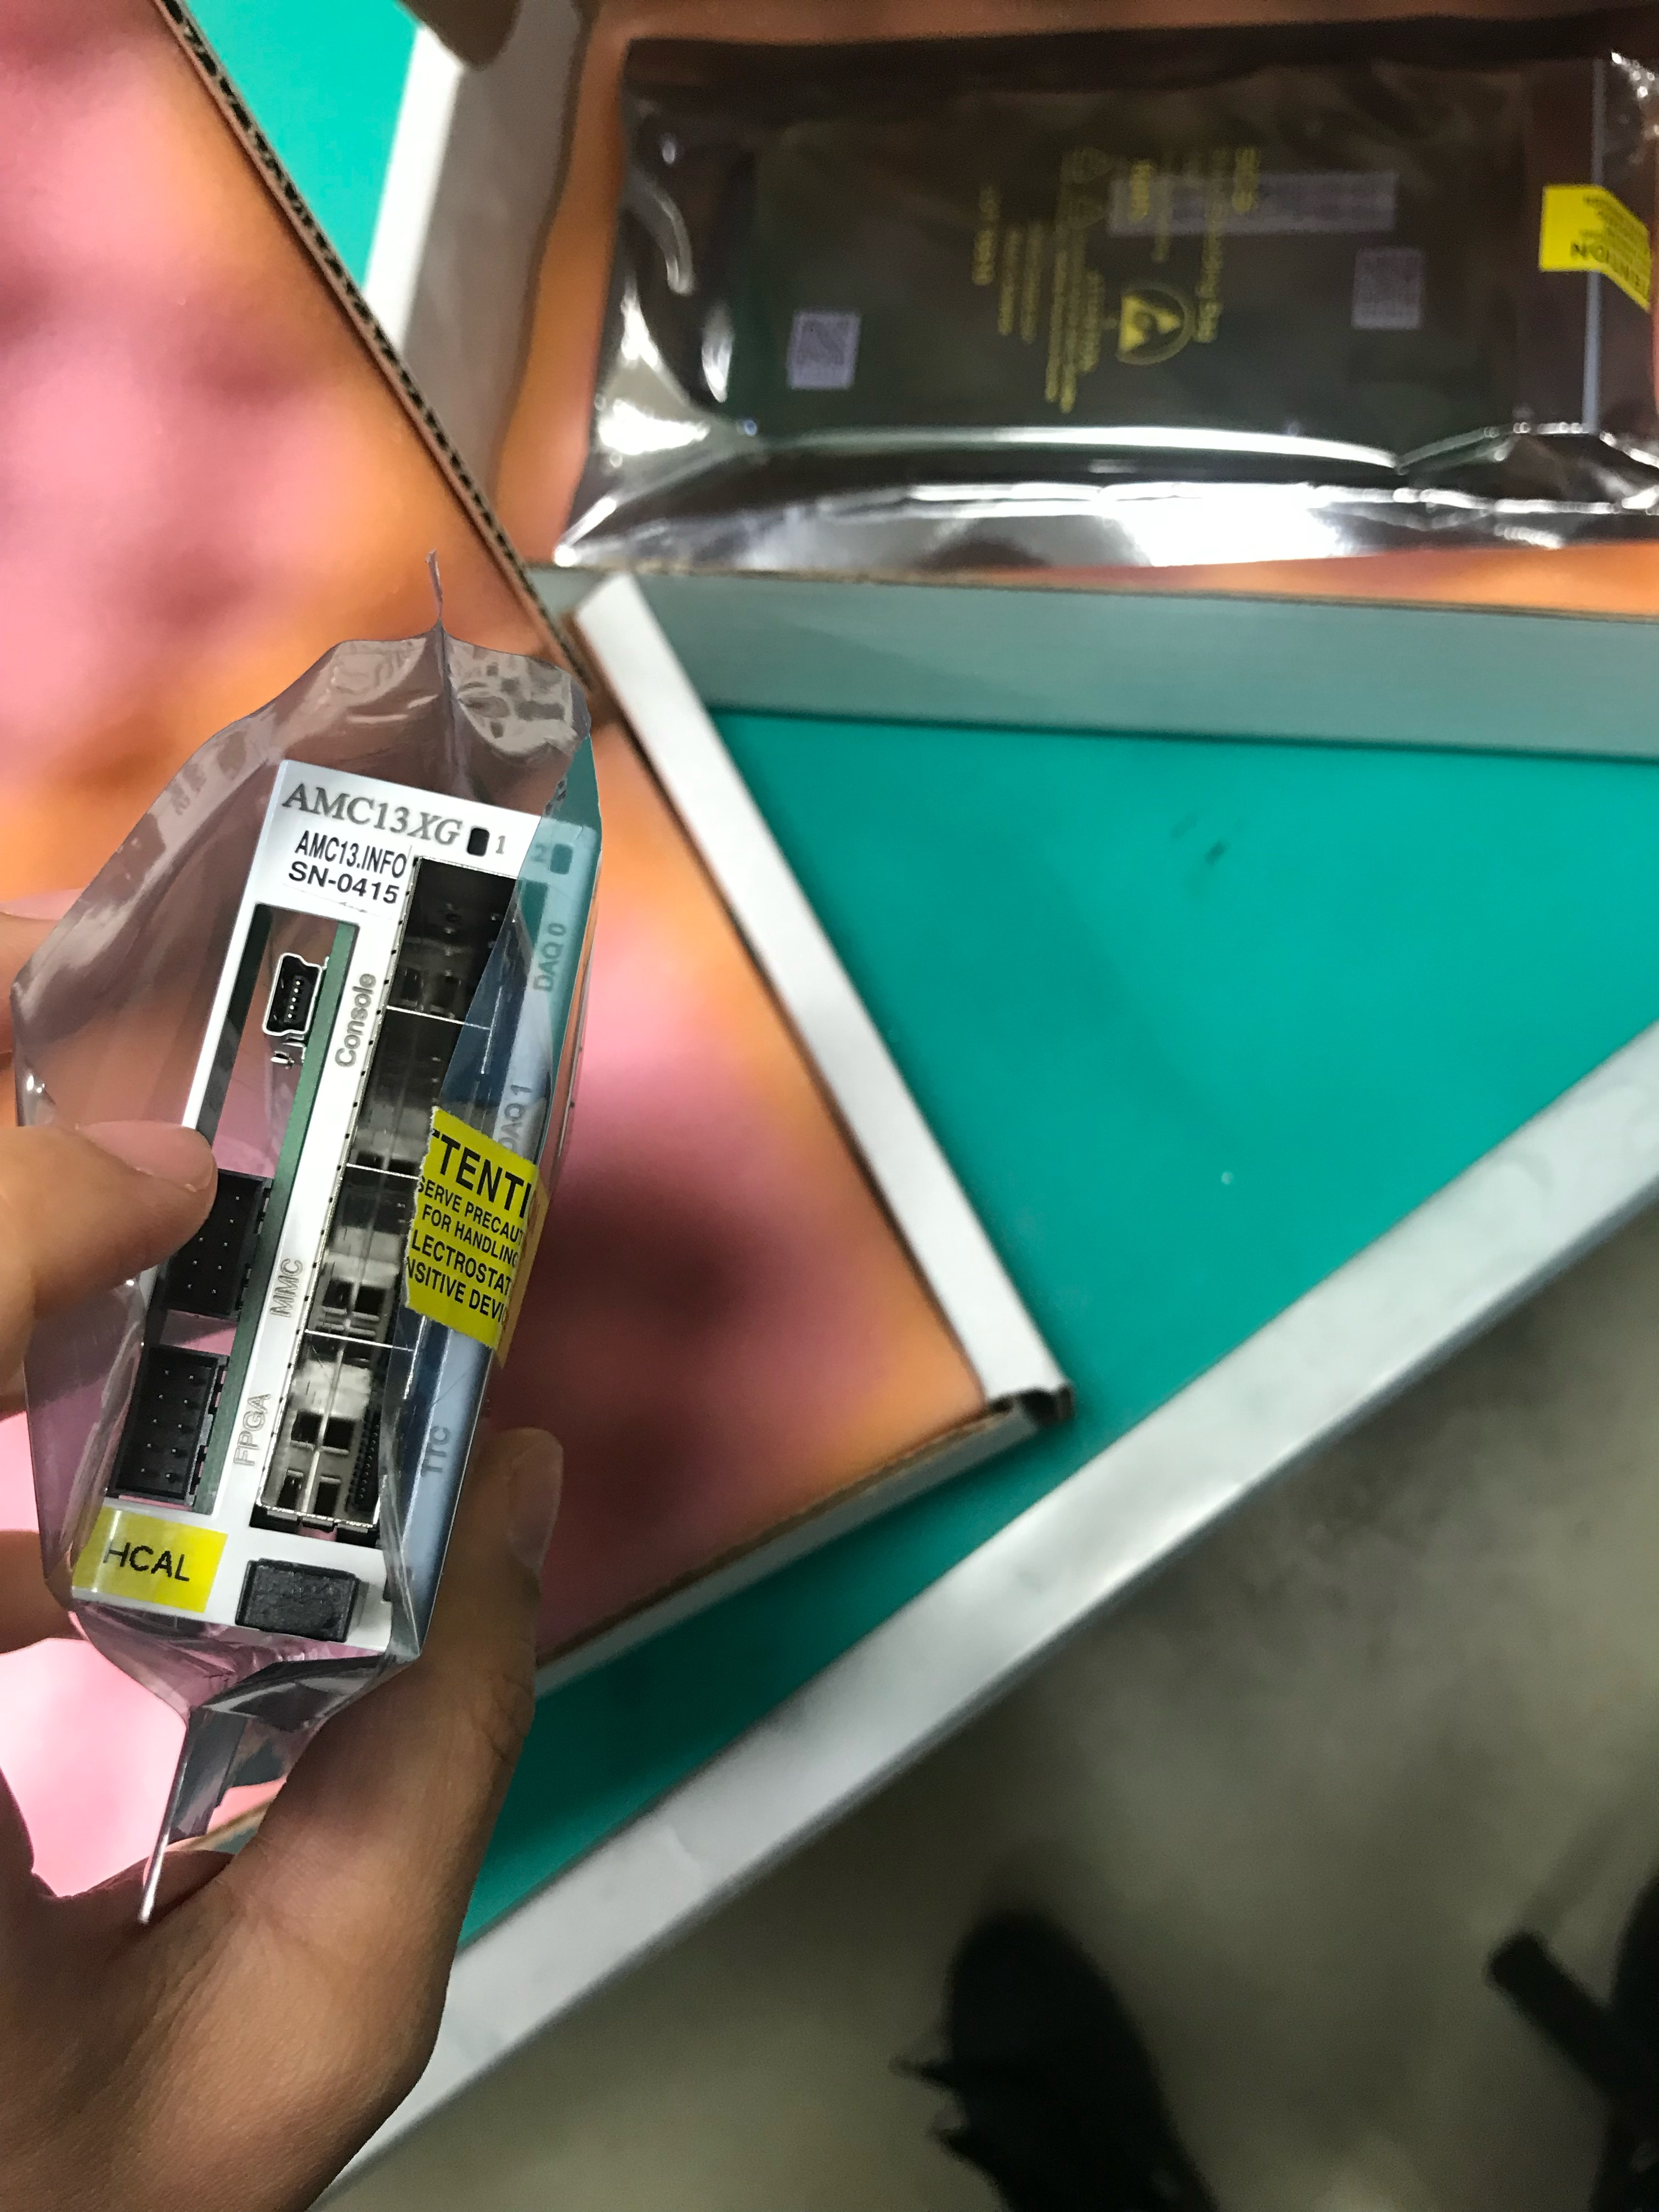
\includegraphics[scale=0.07]{fig/AMC13Reprogramming.jpg}
 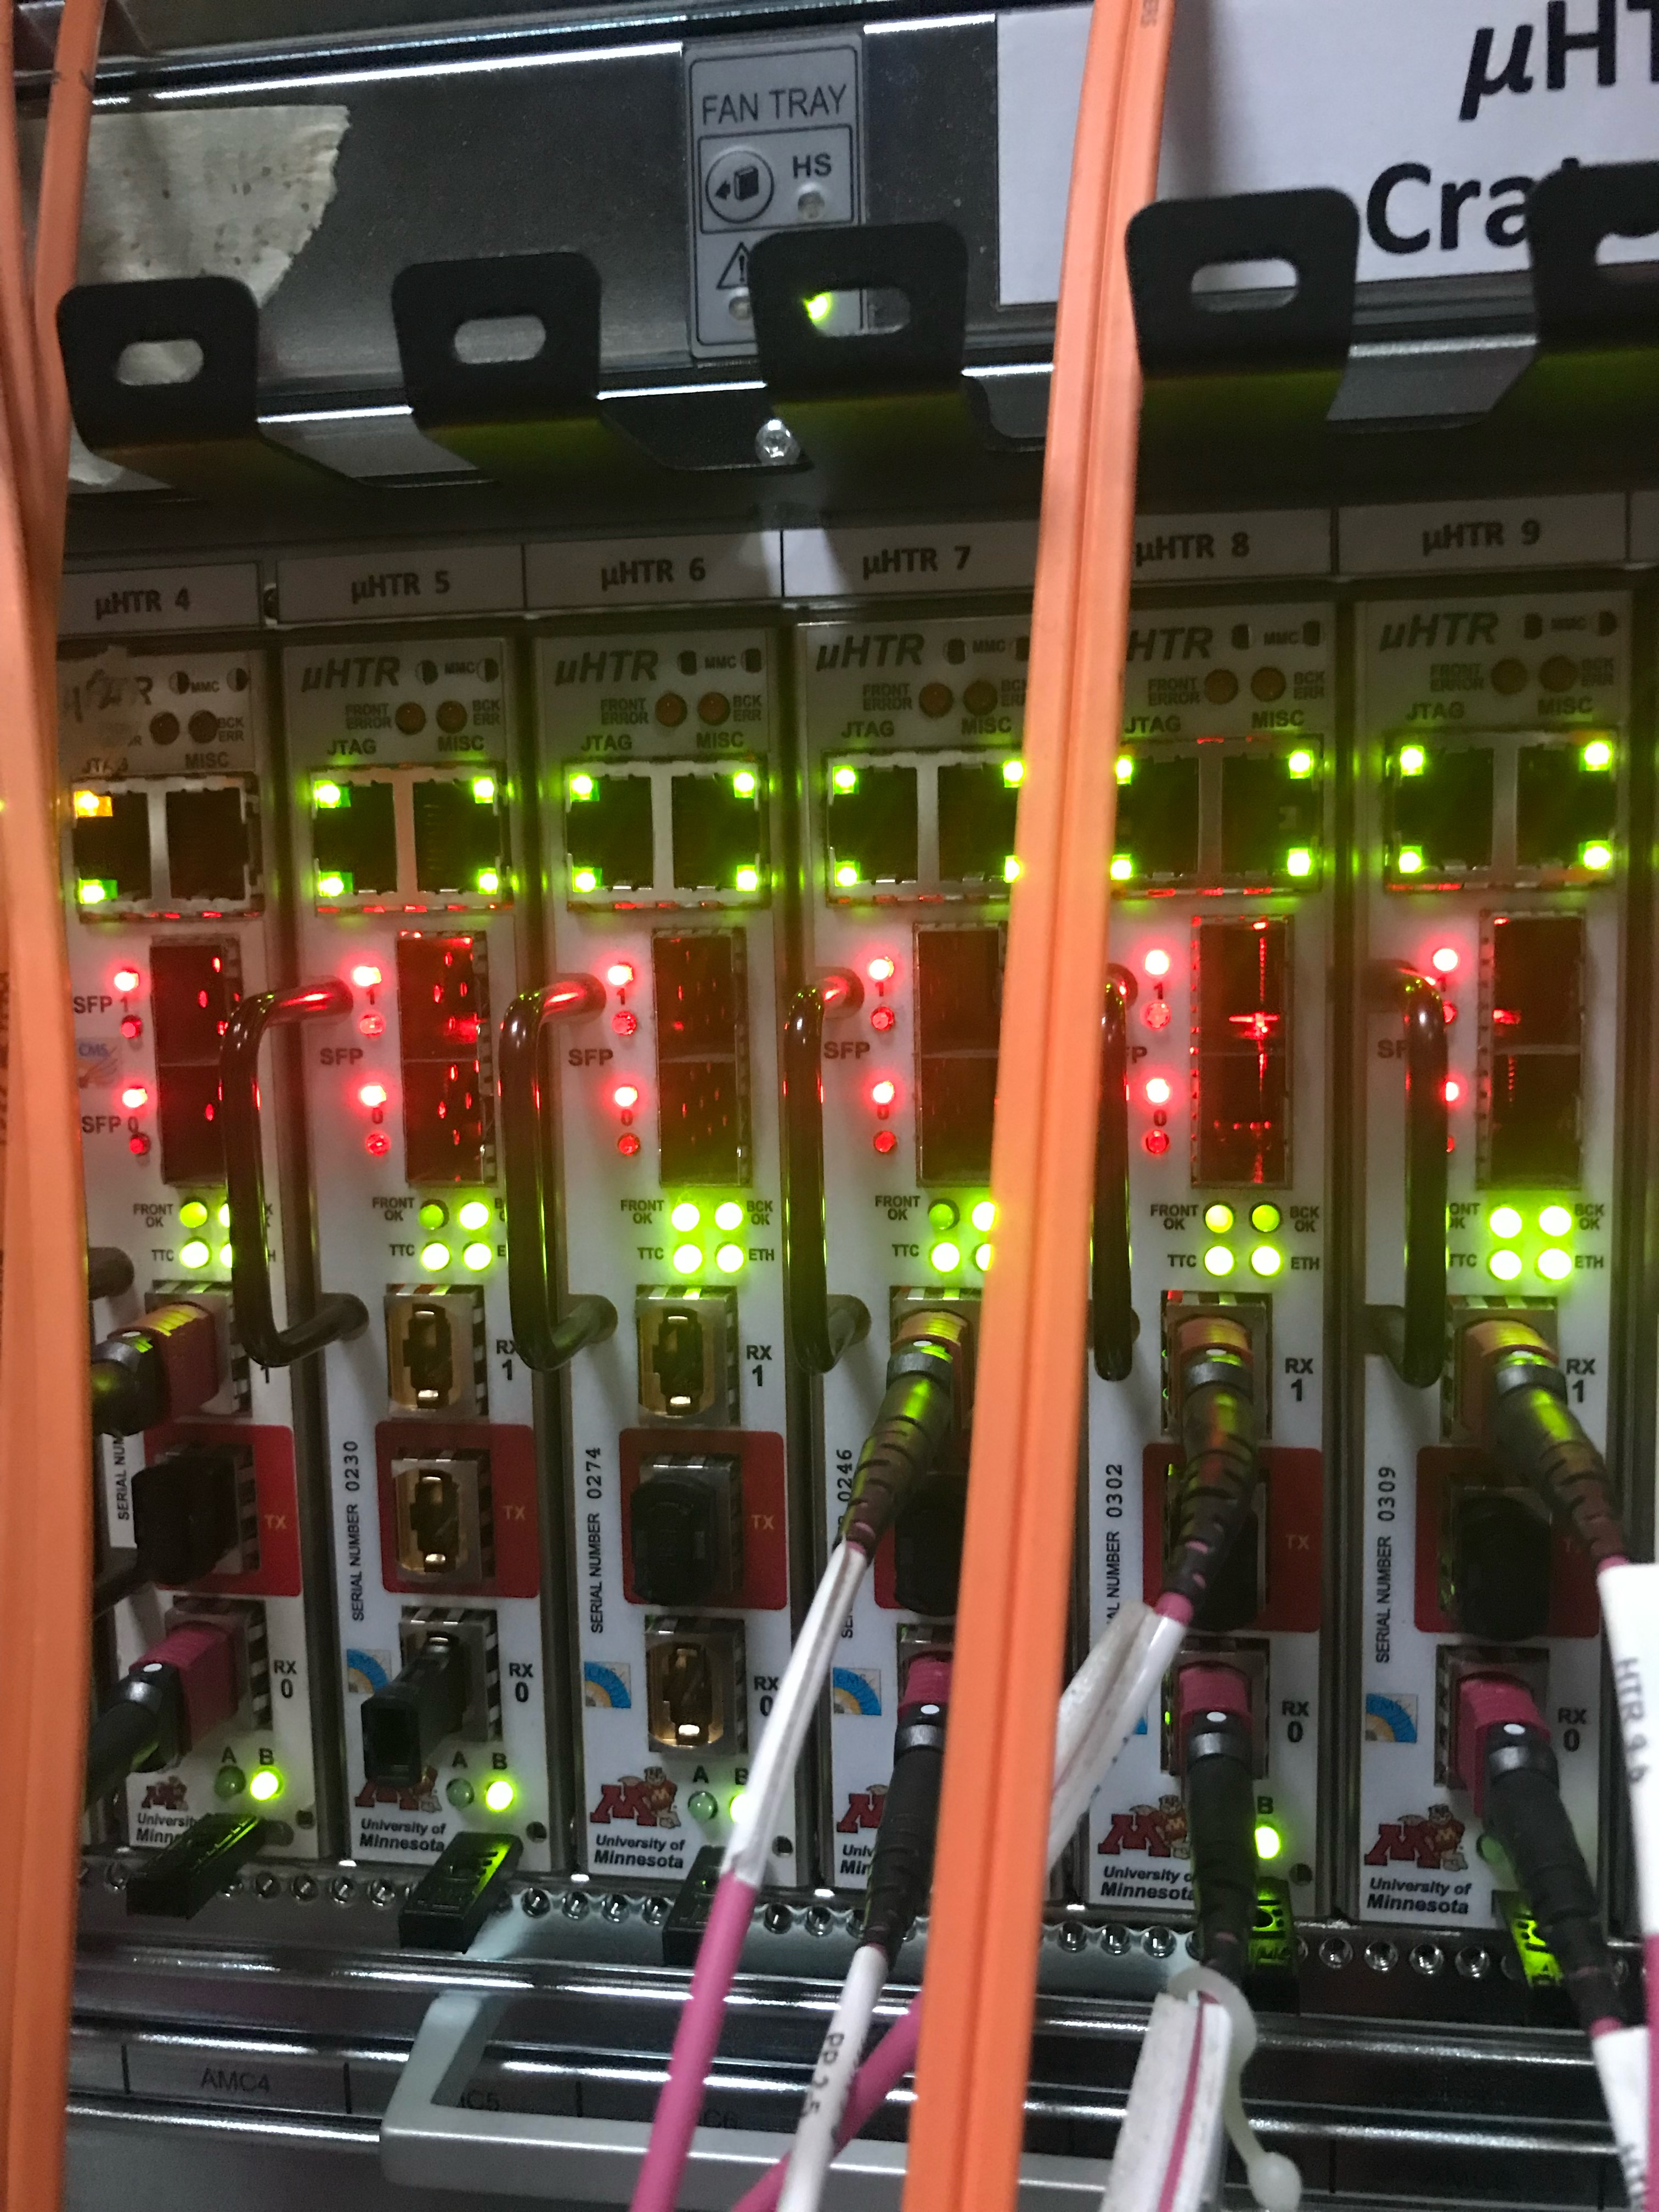
\includegraphics[scale=0.07]{fig/904BE.jpg}
	\caption{On the left is a new AMC13 tested at 904 with the $\mu$HTRs in a selected Back-End Crate shown on the right.}
	\label{fig:BackendCrate9041}
\end{figure}

\begin{figure}[!htb]
	\centering
	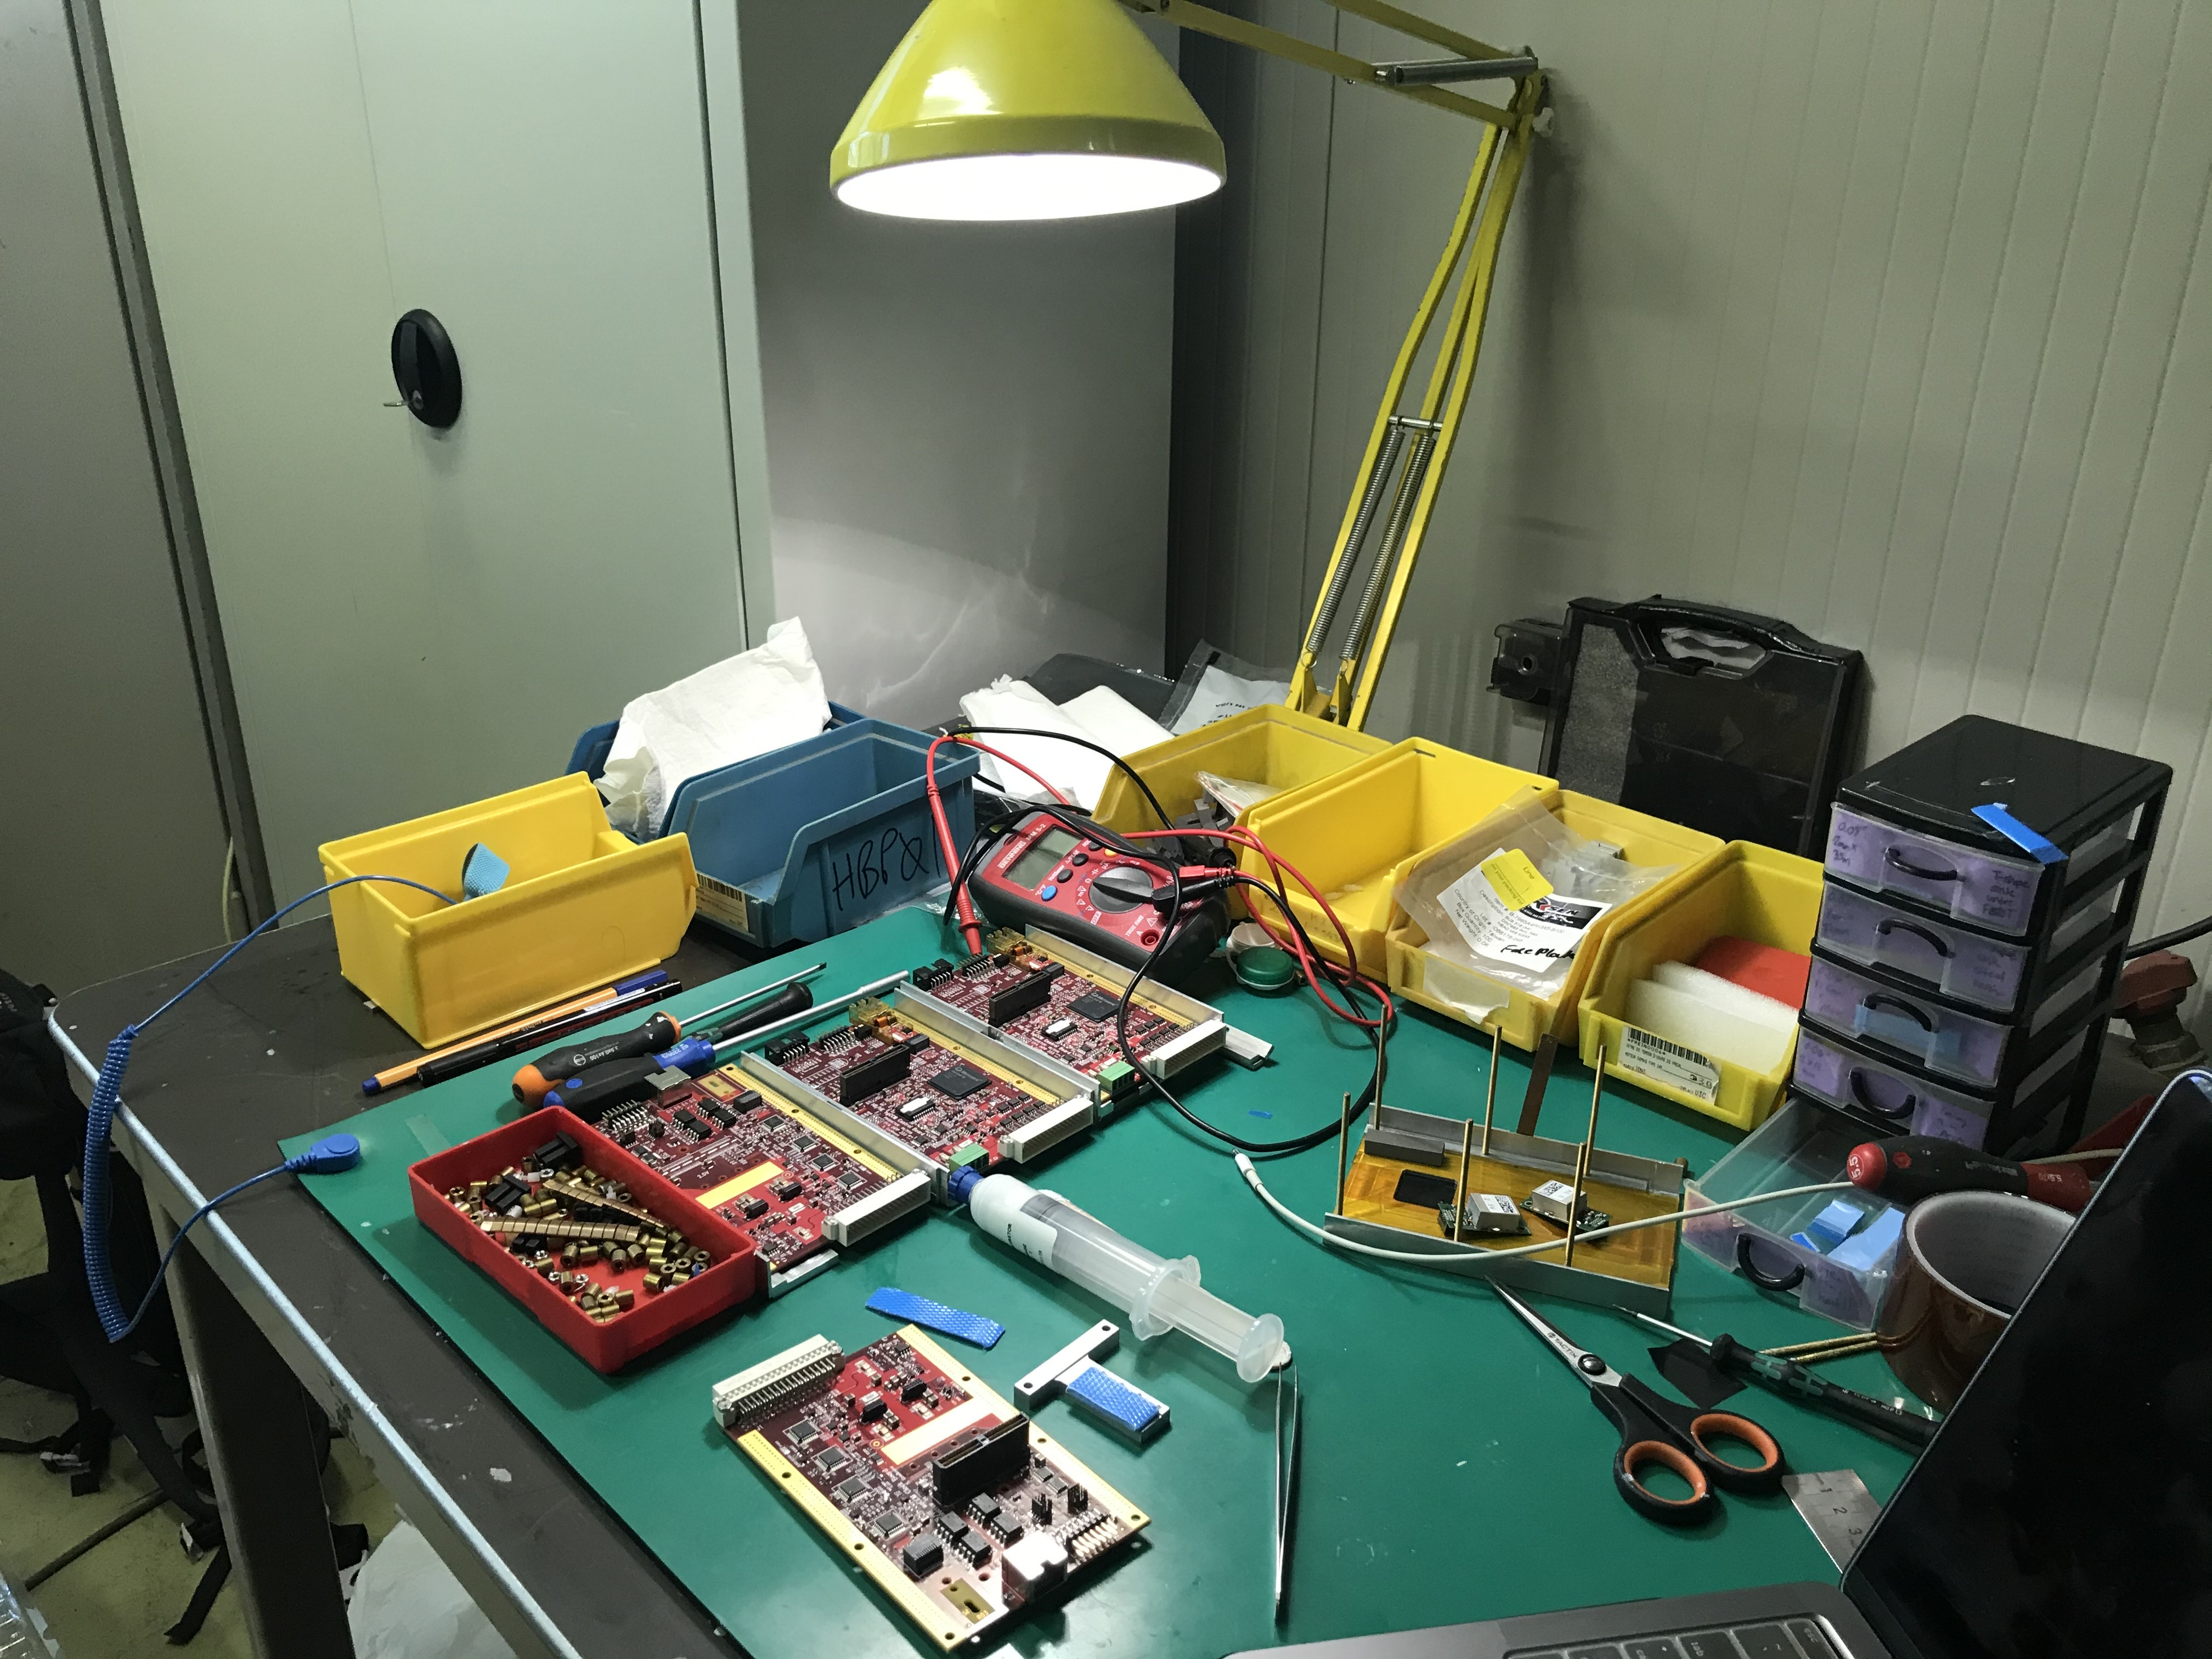
\includegraphics[scale=0.08]{fig/coolingfins.jpg}
     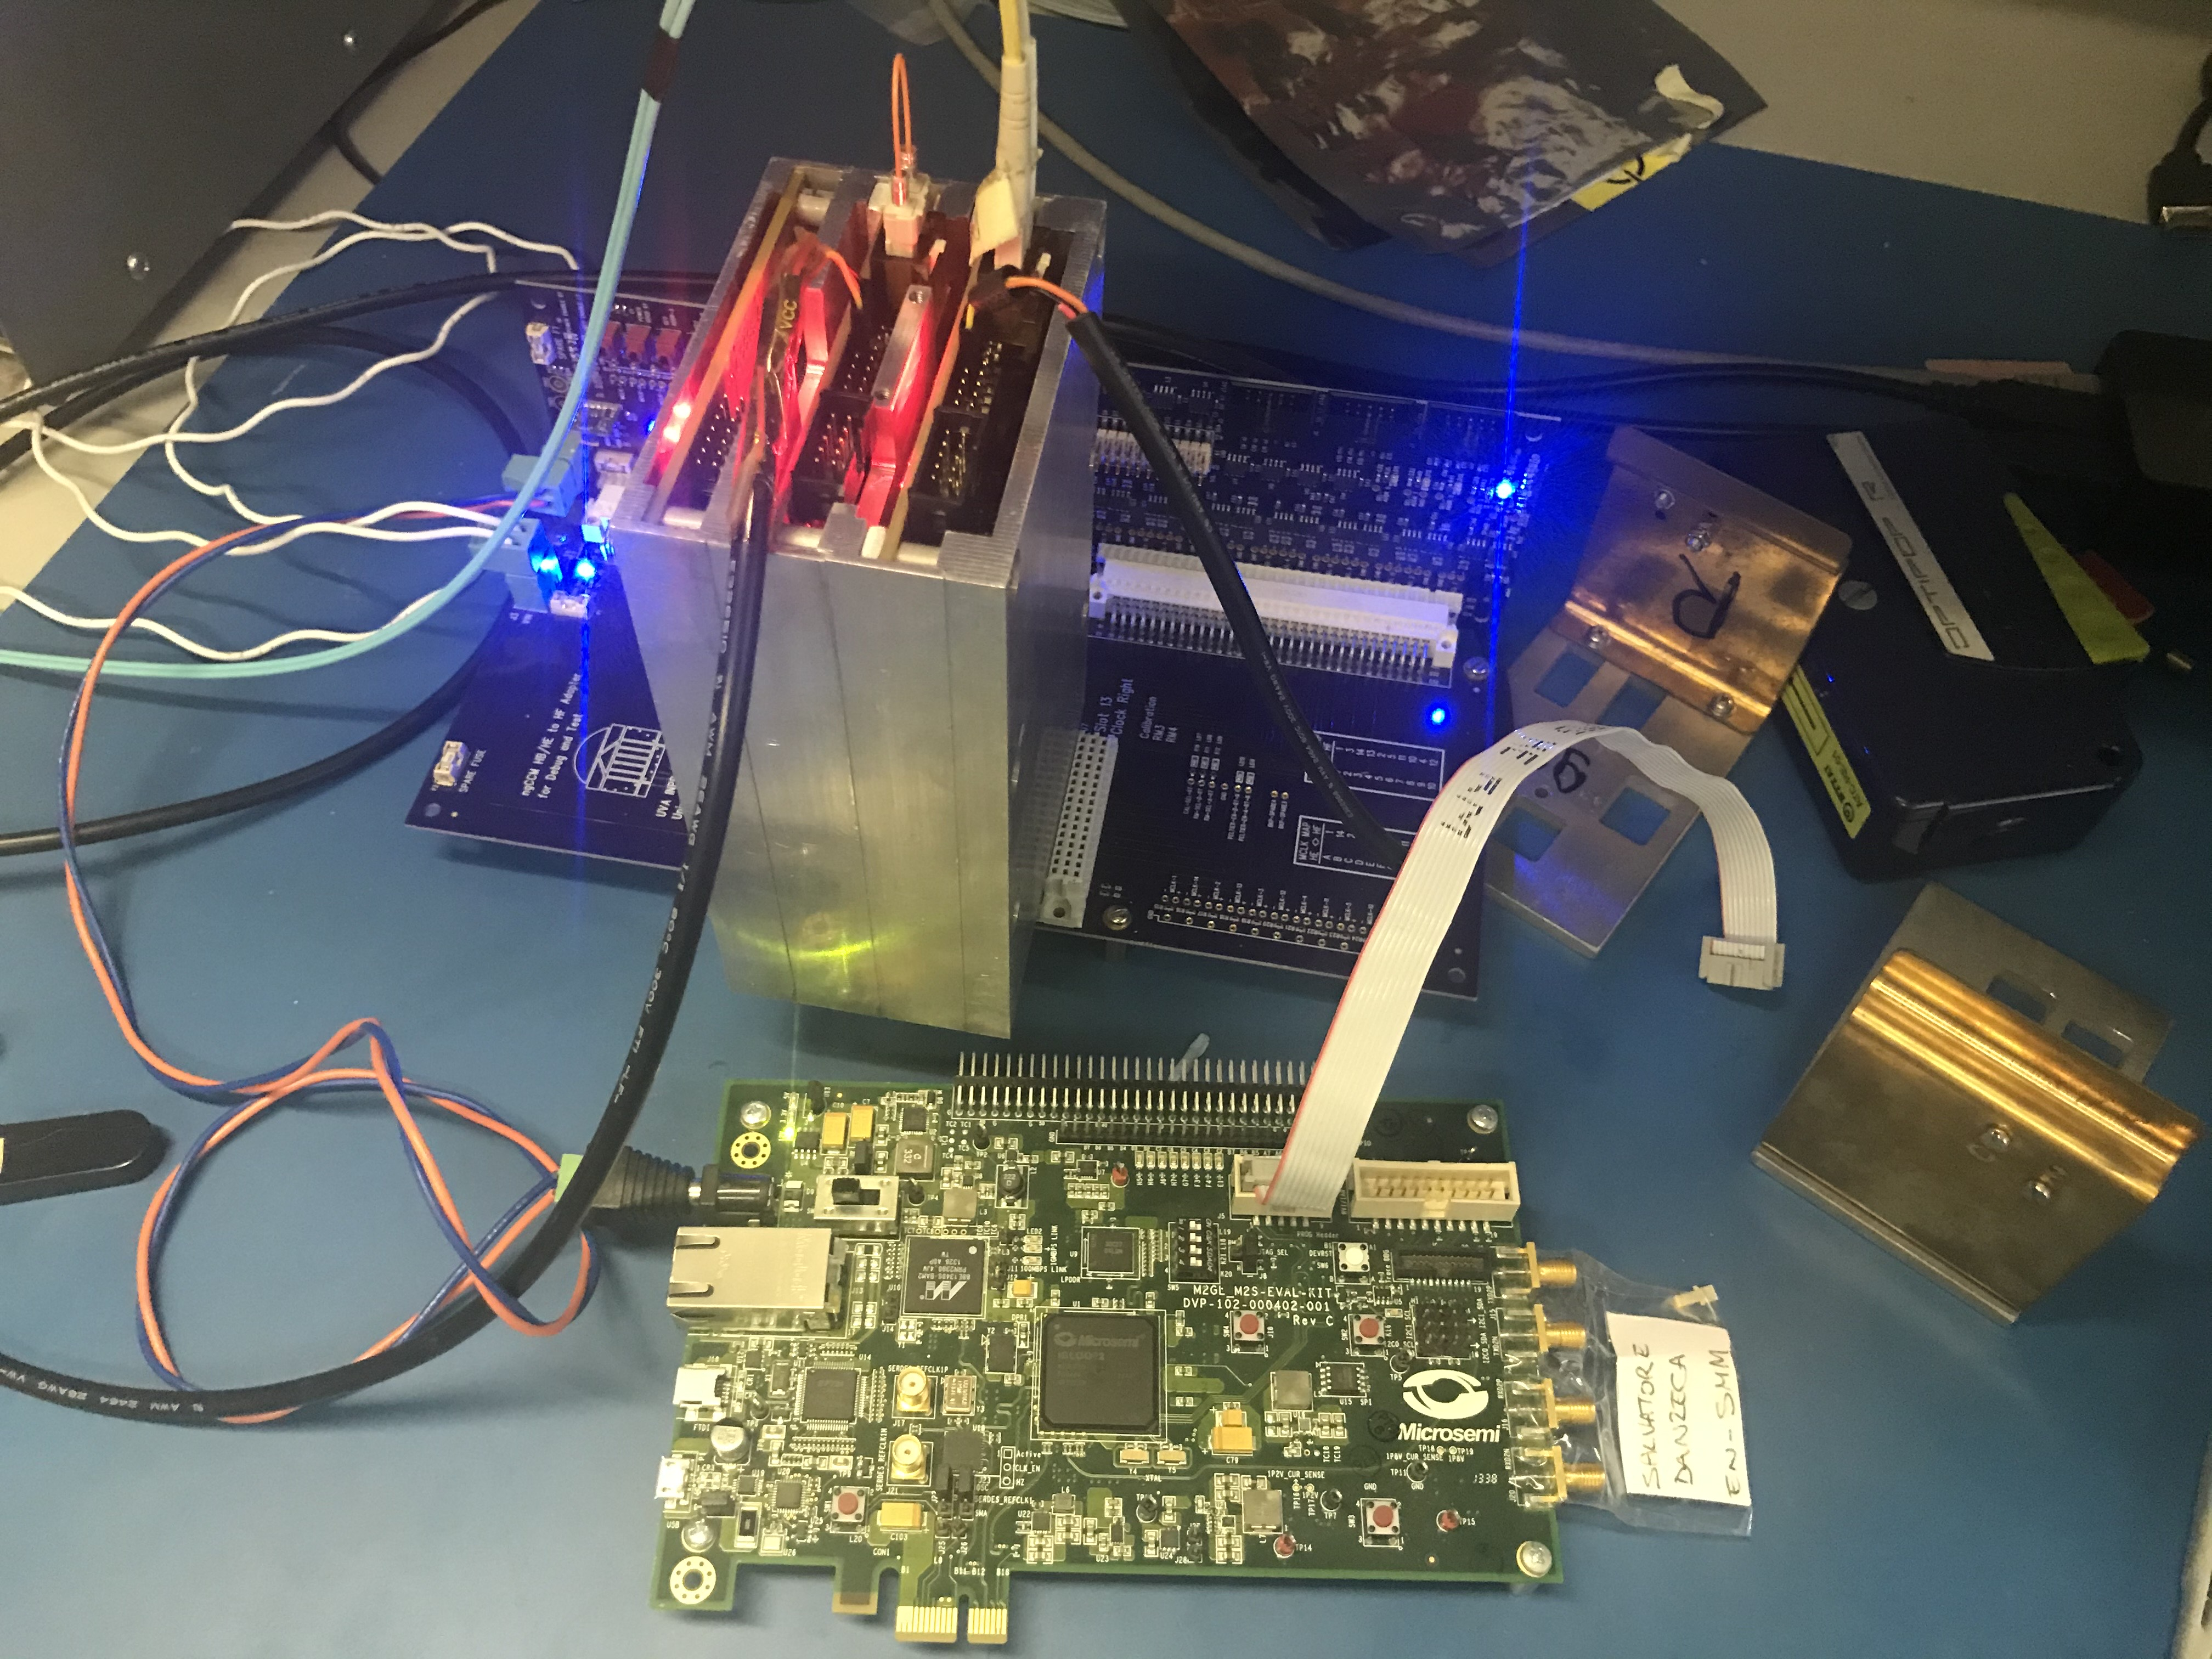
\includegraphics[scale=0.08]{fig/testing.jpg}
	\caption{The top picture shows an ngCCM being reworked to add heat sinks to mitigate the VTRx RSSI drift issue which was related to the communications loss in the HCAL endcap. The right shows a reworked ngCCM being tested on a spare backplane.}
	\label{fig:BackendCrate9042}
\end{figure}

\begin{figure}[!htb]
	\centering
	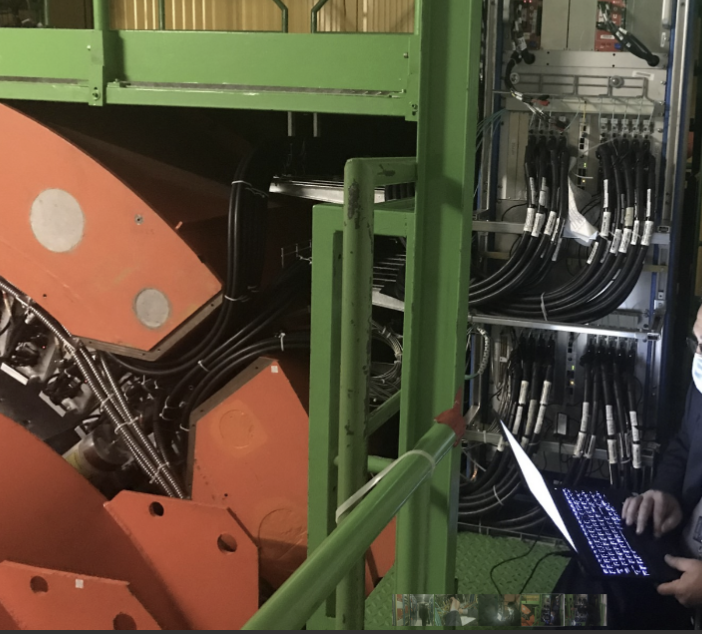
\includegraphics[scale=0.7]{fig/HFIglooReprogramming.png}
	\caption{Reprogramming of the HF Igloo mounted on the HF ngCCMs at the CMS cavern.}
	\label{fig:HFIglooReprogramming}
\end{figure}

\subsubsection{HB TDC LUTs Support for Long-lived Particles}

CMS can take full picture events at 40 MHz but can only record ~1000 full events per second. The idea is to construct a Level-1 (L1) Hardware trigger using the HCAL TDC information within each bunch crossing of 25 ns. Currently, hadronic Long-Lived Particle (LLP) trigger can cover lifetimes greater than ns or microseconds. It is currently at L1 trigger level where the heaviest contstraint lies when it comes to distinguishing prompt particles from long-lived ones. 

\begin{figure}[tbp!]
\begin{center}
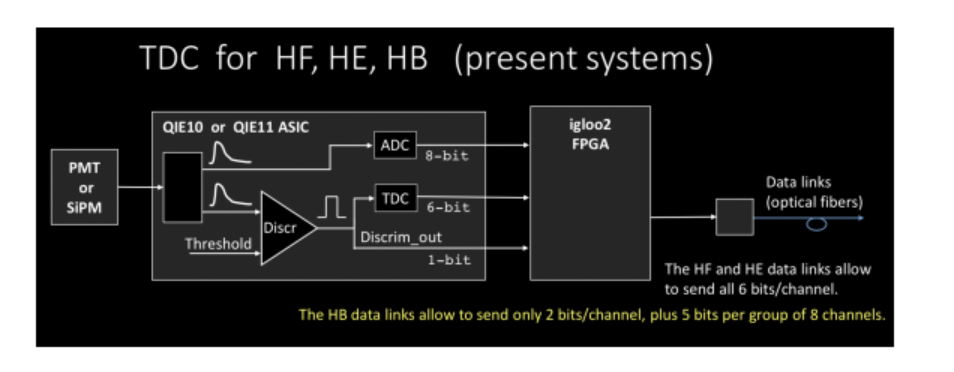
\includegraphics[scale=0.9]{fig/TDCLLP.png}
\end{center}
\caption{TDC Current support Credits: Tullio Grassi}
\label{fig:TDCHBLimits}
\end{figure}

\begin{figure}[tbp!]
\begin{center}
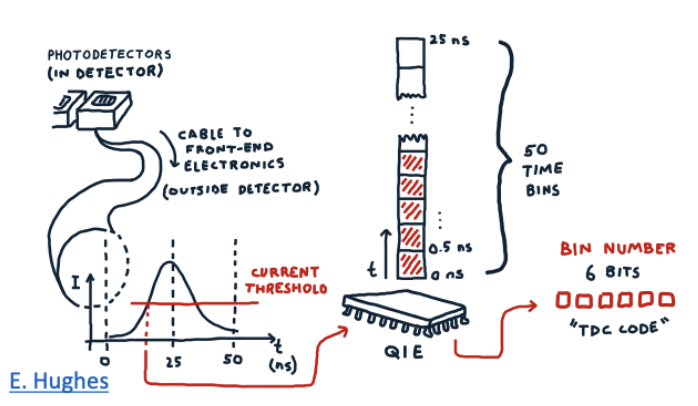
\includegraphics[scale=1.2]{fig/TDCCode.png}
\end{center}
\caption{With the Phase I Upgrade, each QIE channel now has a time-to-digital converter (TDC) which sends out a 6-bit TDC Code. Credit: E.Hughes}
\label{fig:L1TriggerSketch}
\end{figure}

One way to workaround this constraint is to take advantage of the limited bandwidth information. In the HB, only 2 bits/channel are allowed to be sent from the Front-End (FE) electronics to the Back-End (BE) (see Figure~\ref{fig:TDCHBLimits}). This constraint does not exist for both the HE and the HF where the full 6 bit/ channel are transmitted through the data links from FE to the BE. In the Phase I upgrade, each QIE channel now has a time-to-digital converter (TDC), that sends out a 6 bit code.  This is illustrated in a schematics shown in Figure~\ref{fig:L1TriggerSketch}. The Igloo2 FPGAs pack the 6-bit information into meaningful 2-bit information through physics Look-up tables (LUTs). In computer science, Look Up Tables maps keys to some value. In this context, the LUTs map the available TDC codes to the time windows within the bunch crossing of interest. Previously, these LUTs were only hard-coded mappings from the 6-bit to 2-bit information. There are several disadvantages to this. One, the FPGA Igloo2 Firmware would need to be updated each time a new Look Up Table is to be used or investigated. Updating the firmware could be time consuming and also could run into the danger of turning the hardware into ``bricks" when the updating process is interrupted. Not only are the FPGAs expensive to replace, one would also have to wait for a time-window to be able to replace them manually underground. The idea then is to make the LUTs configurable and loadable prior to each data taking run. 

Currently, the software support we implemented for the HB TDC Look Up Tables, takes in xml files. An example xml file containing the LUTs is shown in  Figure~\ref{fig:XMLFile}. They are indexed by RBX, QIE, RM which has a one-to-one map to the detector coordinates indexed by $\eta$, $\phi$, and depth. 

\begin{figure}[tbp!]
\begin{center}
\includegraphics[scale=0.6]{fig/ExampleLUT.png}
\end{center}
\caption{Sample LUT. The RM index ranges from 1-5, where the 5th is the Calibration Unit. Labeling credits: Gillian Kopp}
\label{fig:XMLFile}
\end{figure}

\begin{figure}[tbp!]
\begin{center}
\includegraphics[scale=0.6]{fig/6bitTo2bitMap.png}
\end{center}
\caption{An example of a 6-bit to 2-bit hardmapping information. Credits: Tullio Grassi}
\label{fig:bitMapping}
\end{figure}

An example of a 6-bit to 2-bit mapping as shown in Figure~\ref{fig:bitMapping}. The 6-bit TDC code information comes from the QIE11, which is the processed output of the silicon photomultiplier pulse coming from the detector. Each bunch crossing happens every 25 ns, so the TDC values range from 0-49 in half ns steps to cover the whole time range. Additional error codes are also encoded for example in cases where the pulse starts high (62) or starts low and stays low 
(63).

The 6-bit TDC address from QIE11 is packed into 2-bits in the IGLOO2 firmware LUT, to encode the
following 4 states:

\begin{itemize}
  \item 00 prompt pulse:    $ TDC \leq t_{p}$
  \item 01 slightly delayed pulse: $ t_{p} < TDC \leq t_{p} +2$
  \item 10 very delayed pulse:  $ t_{p} +2 < TDC < 50$
  \item 11 invalid pulse: $ TDC > 50$
\end{itemize}

To determine exactly the time boundary between the states is ascertained from the the distribution of TDC values in a prompt QCD sample and is currently being studies as of time of writing~\cite{HBTDCLUT_uHTR}. One of the potential downsides of loading LUTs was the effect on the configuration time. Prior to every run, the configuration of the various electronics components are set. The new software version was tested at P5 and only an average of 7s was added to the Configuration time. 

% \FIXME{Wishlist: Muon System, References, How the megatiles are grouped together}

% Phase 1 is the system after upgrades installed during Long Shutdown 2 (LS2) of the LHC, between Run 2 and Run 3 of 13 TeV (13.6) TeV running. After the completion of Run 3, the LHC itself will transition to the High Luminosity LHC (HL-LHC). The running conditions of the HL-LHC dramatically differ from those informing the Phase 0 design. Phase 2 upgrades will complete CMS’s preparation for the high luminosity Run 4, and will be installed during Long Shutdown 3 (LS3).
% My work has encompassed almost the entirety of the CMS HCAL Barrel upgrade: the first PCB tests, installation, operations, and finally solving a mystery that ulti- mately impacted a large part of the High Energy Physics community. The following sections describe my contributions to the upgrade effort. First, Section 4.1 intro- duces the HCAL design and upgrade goals. Section 4.2 describes my roles within the HCAL Barrel Upgrade. Finally, Section 4.3 recounts the VTRx (Versatile Link Transmitter/Receiver) failure investigation.

% -------
% Phase I Upgrade of the CMS Hadron Calorimeter
% Seth I. Cooper on behalf of the CMS Collaboration
% Abstract
% In preparation for Run 2 (2015) and Run 3 of the LHC (2019), the CMS hadron calorimeter has begun a series
% of ambitious upgrades. These include new photodetectors in addition to improved front-end and back-end readout
% electronics. In the hadron forward calorimeter, the existing photomultiplier tubes are being replaced with thinner
% window, multi-anode readout models, while in the central region, the hybrid photodiodes will be replaced with silicon
% photomultipliers. The front-end electronics will include high precision timing readout, and the back-end electronics
% will handle the increased data bandwidth. The barrel and endcap longitudinal segmentation will also be increased.
% This report will describe the motivation for the upgrade, its major components, and its current status.

% % https://indico.cern.ch/event/863077/contributions/3850846/attachments/2045904/3427672/llpWorkshop7CMSTriggerV3.pdf


% The Hadron Calorimeter plays an important role in the reconstruction of events in CMS, most notably as the only subdetector capable of measuring neutral hadrons. The hermetic design of the calorimeter allows for the reconstruction of missing trans- verse momentum, a feature that augments HCAL’s existing roles in the calorimeter- based L1-triggers and in electron identification. With the unprecedented luminosity conditions of the HL-LHC on the horizon and the shortcomings of the original front end electronics degrading performance, CMS decided to replace the HCAL front end during the “Phase 1 Upgrade.”
% There are three phases of CMS, each preparing CMS for the next stages of LHC physics. Phase 0 is the originally installed system. 

% In October 2019, the Phase-1 upgrade of the CMS HCAL calorimeter was completed. Each channel now has
% a time-to-digital converter (TDC). The photo-detector technology was changed (hybrid photodiodes were
% replaced with silicon photomultipliers, SiPMs), providing better signal-to-noise performance. In conjunction
% with an increase in the number of readout channels, this allowed a much-improved segmentation in calorime-
% ter depth (longitudinal segmentation). Instead of the previous 1 or 2 (2 or 3) longitudinal readout segments
% in the barrel (endcap) HCAL detector, there are now 4 (up to 7).
% The HCAL trigger is based on the HCAL calorimeter towers. The calorimeter trigger towers in HBHE are
% typically comprised of physical calorimeter towers ganged together in depth. The HCAL trigger primitives
% (TPs) are formed for each trigger tower by combining the information from individual calorimeter towers.
% In addition to the TP generation in HBHE, six “extended bits” of information are also generated that can
% be transmitted to the Level-1 trigger. The meanings of these extended bits (or feature bits) aim to facilitate
% encoding of information about: (i) the longitudinal shower profile data, and (ii) the shower time data
% constructed from the two bits of the TDC information available in each constituent channel of the trigger
% tower. Configurable look-up tables determine which time windows within the BX of interest are represented
% by the available TDC codes. These time window boundaries have a granularity of 0.5 ns. Feature bits as
% determined by the TDC timing or shower profile data can be used to mark hits from late times or from
% distinctive energy deposits in the various layers of the HCAL respectively, that are characteristic of signals
% from long lived exotic particle decays.
% These bits allow the deployment of high efficiency hadronic triggers in Run 3 (and Run 4) operation, and
% are able to capture decays from long lived particles with lifetimes relevant to decays prior to and within the
% HCAL calorimeter volume.








% \section{CMS Experiment - Data Acquisition and Processing}
% The CMS apparatus~\cite{CMS:2008xjf} is a multipurpose, nearly hermetic detector, designed to trigger on~\cite{CMS:2020cmk,CMS:2016ngn} and identify electrons, muons, photons, and (charged and neutral) hadrons~\cite{CMS:2020uim,CMS:2018rym,CMS:2014pgm}. A global "particle-flow" (PF) algorithm~\cite{CMS:2017yfk} aims to reconstruct all individual particles in an event, combining information provided by the all-silicon inner tracker and by the crystal electromagnetic and brass-scintillator hadron calorimeters, operating inside a 3.8\unit{T} superconducting solenoid, with data from the gas-ionization muon detectors embedded in the flux-return yoke outside the solenoid. The reconstructed particles are used to build \PGt leptons, jets, and missing transverse momentum~\cite{CMS:2018jrd,CMS:2016lmd,CMS:2019ctu}. 

% The central feature of the CMS apparatus is a superconducting solenoid of 6\unit{m} internal diameter, providing a magnetic field of 3.8\unit{T}. Within the solenoid volume are a silicon pixel and strip tracker, a lead tungstate crystal electromagnetic calorimeter (ECAL), and a brass and scintillator hadron calorimeter (HCAL), each composed of a barrel and two endcap sections. Forward calorimeters extend the pseudorapidity coverage provided by the barrel and endcap detectors. Muons are measured in gas-ionization detectors embedded in the steel flux-return yoke outside the solenoid. A more detailed description of the CMS detector, together with a definition of the coordinate system used and the relevant kinematic variables, can be found in Ref.~\cite{CMS:2008xjf}. 

% \subsection{Trigger}
% Events of interest are selected using a two-tiered trigger system. The first level (L1), composed of custom hardware processors, uses information from the calorimeters and muon detectors to select events at a rate of around 100\unit{kHz} within a fixed latency of about 4\mus~\cite{CMS:2020cmk}. The second level, known as the high-level trigger (HLT), consists of a farm of processors running a version of the full event reconstruction software optimized for fast processing, and reduces the event rate to around 1\unit{kHz} before data storage~\cite{CMS:2016ngn}. 

% \subsection{Offline Analysis}
% \section{CMS HCAL Online Software and Electronics}
% Upgrade \cite{Cooper:2016kef}
% VTRX communications loss \cite{Cummings:2022kgm}

% The total integrated luminosity of Run 2 is known with a better relative uncertainty than that of the partial data taking periods. Here is a sentence that could be used in standard papers:

% The integrated luminosities for the 2016, 2017, and 2018 data-taking years have 1.2--2.5\% individual uncertainties~\cite{CMS-LUM-17-003,CMS-PAS-LUM-17-004,CMS-PAS-LUM-18-002}, while the overall uncertainty for the 2016--2018 period is 1.6\%.

% In case the 2015 data is included in the analysis, the sentence above should mention "2015--2018", everything else remaining identical.

% Physics coordination would like to see a citation to the paper CMS-LUM-17-003 in all CMS papers. The BibTeX for the other two PASes is also given below. 





        
\newpage
% \section{References}
% \renewcommand{\bibsection}{}%removes the spaces and unwanted references heading from the list
% \begin{singlespacing}
% \bibliographystyle{apsrev}
% \bibliography{Ref_LHC_CMS.bib}
% \end{singlespacing}\par
% %{\let\thefootnote\relax\footnote{{Copyright: \copyright 2019 Elsevier B.V.}}}

\chapter{Particle Reconstruction and Event Selection}
The CMS Detector is composed of layers of subdetectors each of which provide information from the footprints left behind by the particles that come out of the collisions. The data across all the subdetectors are complementary and are linked to reconstruct Physics Objects~\cite{Beaudette:2013kbl}. For most CMS analyses, the Particle Flow Algorithm is used to construct idealized representations of physics objects such as photons, electrons, muons and jets. In the algorithm, tracks are first reconstructed through an efficient track reconstruction algorithm. If these tracks fall within a defined boundaries of one or several clusters, these tracks are associated with the cluster via a linking procedure. A separate clustering algorithm is used to disentangle the overlapping showers. Muons that go all the way to the end of detector are determined first as their tracks do not give rise to a charged hadron. Multiple clusters across various subdetectors and have an associated track are considered charged hadrons. The electrons, due to Bremhsstrahlung photon emissions, uses a tailor-made track reconstruction to properly attach these photon cluster to the electron it originated from. This also avoids energy double counting. Once all the tracks have been considered, the remaining clusters without any associated tracks are used to determine the neutral particles. Energy clusters concentrated in the ECAL and without associated tracks, are categorized as photons, the primary physics objects used for this analysis. In the case of neutral hadrons, most of their energies are contained in the HCAL. Once the once tracks are linked to appropriate clusters, for charged particles, and the neutral objects are determined, they are linked to the best fit primary vertex, the nature of the particles are assessed and a four-momenta is calculated. Further details on the Particle Flow Algorithm and other physics objects are found in~\cite{CMS-PRF-14-001}.

In this analysis, the events of interest are those with two high-energy, prompt photons. The events containint this signature are first required to pass a trigger selection and an offline reconstruction is performed. To obtain even higher purity and higher search sensitivity, these diphoton candidates are required to pass additional pre-selection and various levels of identification criteria called photon IDs. 

In the succeeding pages we discuss the Particle Flow elements and Particle Reconstruction, event selection, triggers used in this analysis. The second half of the chapter will discuss the the Photon ID~\ref{subsec:photonID} used for high-mass diphoton events, the data sets used for the analysis as well as the known detector issues that might affect the results of the analysis. 

% In the succeeding pages we discuss the Particle Flow elements and Particle Reconstruction in Sec.~\ref{sec:PFelements}. Sec.~\ref{sec:Ev} discusses the event selection, triggers used in this analysis. Sec.~\ref{subsec:photonID} discusses the Photon ID used for high-mass diphoton events. In the last section, we discuss the selection efficiency for our chosen cuts.

\section{PF Elements and Phyics Objects}~\label{sec:PFelements}
The Particle Flow (PF) elements are the basic building blocks used for particle reconstruction for CMS. These are mainly the \textit{Tracks and Vertices} and the \textit{Calorimeter Clusters}. The PF algorithm makes use of the track and vertices to identify and measure the momentum of charged particles and also identify displaced vertices, particularly from b-quark jets. The energy deposits in the calorimeters are clustered by the algorithm and used to identify neutral particles such as photons. These are also used to augment the reconstruction of physics objects like electrons and charged hadrons in jets. The information from the vertices, tracks and clusters are then chained, to the best estimate of the algorithm to form the basic physics objects. This is shown in a schematic in Figure~\ref{fig:CMSParticleFlow}. More detailed information on the algorithm is found in reference~\cite{CMS-PRF-14-001}. While not used in this dissertation, it is interesting to note that novel machine learning methods have recently been developed to directly exploit detector level data without going through the hand-engineered features that the particle flow algorithm has to categorize particles~\cite{Andrews_2020_e22_jet, Andrews_2020_e2e_direct}.

% \FIXME{Wishlist: Describe a little more how the PF elements are formed just for fun.}

\begin{figure}[!htb]
	\centering
	\includegraphics[scale=0.6]{fig/CMSParticleFlow.png}
	\caption{The information from the vertices, tracks and calorimeter energy deposits are chained by the PF algorithm to form the various physics objects.}
	\label{fig:CMSParticleFlow}
\end{figure}

For this analysis, we are mostly interested in photons, muons and jets. We are interested in signal events containing two photons and some of our background estimates are derived from jet and muon datasets. 


\subsection{Tracks and Vertices}\label{sec:track_vertex}

Charged particles leave tracks as they propagate through the Silicon tracker layers. These tracks are fundamental as they contribute towards the subsequent reconstruction of other physics objects in an event. CMS makes use of the Combinatorial Track Finder algorithm (CTF) based on a Kalman filter to reconstruct tracks by fitting tracker hits taking into account hit position uncertainty and the effects of multiple Coulomb scattering and energy loss. The fit then returns the track information incuding the charge, initial momentum of the particle as well as the impact parameter with respect to the primary vertex. This process is described in more detail in Ref.~\cite{Chatrchyan:2014fea}.

The primary vertex is determined based on its compatibility with the hard scattering from the pp interactions along the beam line. In each event, there are accompanying secondary vertices resulting from particle decays after the hard interaction. To reconstruct the primary vertex, tracks that are compatible with the LHC beam spot are selected and clustered. The LHC beam spot corresponds to the 3D luminous region where the LHC beams collide. The track clustering algorithm is described more in Ref.~\cite{Chatrchyan:2014fea}. Due to pileup, multiple primary vertices can be reconstructed in an event but the main primary vertex is chosen such that it has the largest summed charge particle track $\pt^2$, with some additional constraints described. Ref.~\cite{CMS:2014pgm} gives more details on the deterministic annealing algorithm used for vertex reconstruction. Their result also achieved a position resolution of 10-12 $\mu$m in each of the three spatial dimensions for the reconstructed primary vertices for interesting \Pp collisions. 

\subsection{Photon and Electron Reconstruction}~\label{sec:PhotonAndElectronRECO}
Photon candidates are reconstructed from energy deposits in the ECAL that typically do not have any associated tracks in the tracker. Individual energy deposits are grouped into superclusters~\cite{Khachatryan:2015iwa} that are compatible with the expected shower shape extending along the azimuthal ($\phi$) direction. This allows for the recovery of the energy deposited by bremsstrahlung and photon conversions. The clustering algorithm does not make any hypothesis as to whether the particle originating from the interaction point is a photon or an electron. Thus the same algorithm used for photon reconstruction can be applied to $Z \rightarrow e^+e^-$ events and these events are used to
measure the efficiency of the photon selection criteria and of the photon energy scale and resolution. Additionally, these photons should not have any associated HCAL deposit containing more than $10\%$ of its energy from the ECAL supercluster. Photon Energy reconstruction includes energy corrections that account for detector effects. For the endcap photons, energy from the ECAL preshower are also added to the photon energy measurement. Pileup contamination and photon shower loss are also accounted for. Photon showers may be lost in the gaps between crystals or ECAL modules. To correct for these losses, the photon efficiency is calculated and the differences between efficiencies in data and simulation are corrected using scale factors (see Sec.~\ref{selection_efficiency}). More details on the full process are found in \cite{Mukherjee:2021wzi}. 

% Photon and Electron Reconstruction is performed in various steps starting from the clustering of photon energy in the ECAL and track matching. Corrections are applied as well as the energy scale uncertainty.

% Individual particles in the CMS detector are reconstructed using the particle-flow event algorithm~\cite{CMS-PRF-14-001}.
% A more detailed description of photon reconstruction in the CMS detector can be found in Ref.~\cite{Khachatryan:2015iwa}.

% Photons are neutral particles and should leave no track in the inner tracker. However, photons may also convert in the tracker into an electron-positron pair whose paths bend under the influence of the magnetic field. They leave most of their energy deposits in the ECAL. In cases where their trajectories are bent, the energy deposits are extended along the $\phi$ direction. The energy deposits are grouped into so-called ECAL superclusters with transverse energy $E_{T} > 10 GeV$. Details on the procedures on how these superclusters are formed are found in \cite{PhotonReconstruction_2015}. Additionally, these photons should not have any associated HCAL deposit containing more than $10\%$ of its energy from the ECAL supercluster. 
% Photon Energy reconstruction includes energy corrections that account for detector effects. For the endcap photons, energy from the ECAL preshower are also added to the photon energy measurement. Pileup contamination and photon shower loss are also accounted for. Photon showers are lost in the gaps between crystals or ECAL modules. To correct for these losses, the photon \textbf{efficiency} is calculated and the differences between efficiencies data and simulation are corrected using \textbf{scale factors}. More details on the full process are found in \cite{PhotonAndElectronReco}

% Electrons are reconstructed by associating a clus-
% ter in the ECAL with a track in the tracker. The
% clusters are reconstructed by summing up the en-
% ergy deposits in crystals surrounding the “seed” crys-
% tal, which is locally the crystal with largest energy
% deposit. The summing algorithm incorporates en-
% ergy deposits arising from bremsstrahlung emissions
% in the tracker. Energy clusters in the ECAL are
% matched to hits in the inner tracker, which are then
% used to seed tracks in the rest of the tracking detec-
% tor. A dedicated electron track reconstruction algo-
% rithm, known as Gaussian Sum Filter (GSF) algo-
% rithm, accounts for bremsstrahlung emission before
% the calorimeter. The resulting cluster–track matched
% objects form the final electron candidates. 

% The effi-
% ciency for electron reconstruction is measured with
% the tag-and-probe method [3, 4] by using Z → ee
% events. A tag electron is established by applying
% tight cuts to one electron candidate; the other can-
% didate is used as a probe. A large sample of high-
% purity probes is obtained by requiring that the tag-
% and-probe pair has an invariant mass consistent with
% the Z-boson mass. All efficiencies and scale factors
% described in this article, including trigger efficiency,
% the GSF track reconstruction efficiency in the sili-
% con tracker, electron and photon identification effi-

Electrons being charged particles are reconstructed by associating an ECAL cluster with a track in the tracker. The ECAL clusters are reconstructed by summing up the energy deposits in the crystals around the ``seed" crystal which has largest energy deposit. These clusters are matched to hits in the inner tracker using the Gaussian sum filter (GSF) algorithm. Both the summing and the GSF algorithms take into account the energy deposits arising from the bremsstrahlung emissions in the tracker~\cite{Mukherjee:2021wzi}.

% Electrons being charged particles should leave tracks in the tracker. To reconstruct these objects, the tracks are matched to an ECAL supercluster.  using the same method for photons that convert into electron-positron pairs in the tracker. To date, the standard track reconstruction uses a Gaussian sum filter (GSF) to fit the tracker hits. The GSF also takes account secondary tracks coming from emitted bremsstrahlung photons. More details on the procedure are found in \cite{CMS:2015xaf}.

%% Khachatryan:2015iwa is the same as CMS:EGM-14-001 cited in Detector section
% \FIXME{}
\subsection{Muon Reconstruction}

Muon candidates are reconstructed from information from the muon system and inner tracker. The presence of reconstructed tracks from the outer tracking muon system must satisfy compatibility requirements with a track in the inner tracker. The track segments in the muon system are generated by requiring a certain number of hits in the layers within a single DT or CSC chamber. Within an angular cone of $\Delta R < 0.3$, the summed $p_{T}$ of any additional tracks and calorimeter deposits should not exceed 10$\%$ of the muon track's $p_{T}$. For $p_{T} < 200$ GeV, the muon $p_{T}$ and direction are based on the associated inner track's momentum and direction. Above that, they are based on the best track fit between the inner and outer track, with the information from the RPCs included. More details on the algorithm used are found in Ref.~\cite{CMS:2018rym} 

\subsection{Jets Reconstruction}

Jets are reconstructed from what is left from the pool of PF candidates after isolated photons, electrons, and muons have been identified. These jets are typically reconstructed with the anti-$k_{t}$ algorithm \cite{antikt_algorithm} with a radius parameter $R=0.5$. These candidates are further classified into charged hadrons (e.g. $\pi^{\pm}$, $K^{\pm}$, protons), neutral hadrons (e.g. $K^{0}$) and non-isolated photons ($\pi^{0}$). Non-isolated photons have ECAL clusters that are not linked to any track. Neutral hadrons are also not linked to any track but have energy clusters in the HCAL. Reconstructed tracks matching to ECAL and or HCAL clusters form charged hadrons. Their energy deposits are corrected to account for the nonlinear response of the calorimeters. For $|\eta| > 2.5$, neutral hadrons cannot be distinguished from charged hadrons since that range is beyond the tracker acceptance.  For non-isolated photons or neutral hadrons, their energies are determined by the corrected ECAL or HCAL cluster energy or the combined cluster energy of ECAL and HCAL if $|\eta| > 2.5$. Charged hadron energies are derived from whichever is the larger value between the calorimeter cluster energies or the sum of the matched track momenta \cite{Strologas:2287326}. 

\section{Event Selection}~\label{sec:EventSelection}
This analysis selects events containing two high-energy, prompt photons. To select these events, an online trigger selection, and further offline selection and photon identification criteria are imposed. These further selections ensure that the  photons are well-measured and isolated from other particles in the event, help reduce background from other processes and thereby increase the sensitivity of this analysis. 

\subsection{Trigger Selection}~\label{sec:TriggerSelection}
Events for this analysis are required to pass an online high-level trigger (HLT) selection containing two reconstructed photon candidates each with a transverse momentum $p_{T} > 60 (70)$~GeV in the range $|\eta| < 3.0$ for 2016 (2017/2018). We refer to these as the Double Photon Triggers. Each photon candidate must also have a ratio of the hadronic to the electromagnetic energy (H/E) $<$ 0.15. The electromagnetic energy here is defined as the corrected supercluster energy while the hadronic energy is the total HCAL energy within a cone of $\Delta R <$  0.15 from the supercluster position. This ratio is also the amount of the HCAL energy in the tower directly behind the photon seed crystal. 

To quantify the efficiency of the Double Photon triggers, we use a reference for normalization. This reference trigger selects events that contains two photons each with transverse momentum greater than 33 GeV and satisfies the Calorimeter Identification (CaloId) criteria. The efficiency is primarily a function of the $p_{T}$ of the second-leading photon, the photon which has the second highest $p_{T}$ among the collection of photons. The results are shown in Figure~\ref{fig:trigger_efficiency}. The precise form of the fit is irrelevant as the efficiency plateaus well before the offline cut value. This procedure only probes the turn-on of the $p_{T}$ leg \cite{ref:AN2016_167} have shown that there is no additional source of efficiency and this study serves as a cross-check. An additional backup trigger was also used to mitigate potential efficiency losses at high diphoton invariant masses. We calculated an additional 0.2$\%$ yield over the full analysis region with several thousand events, without viewing any distributions to avoid bias during the blinded phase of the analysis. The trigger efficiency is fully efficient at $p_T > 125$ GeV, which is the photon $p_{T}$ selection used in this analysis. For details on the exact trigger path names see Appendix~\ref{ch:appendix_datasets_triggerpaths}.

% These selection details are contained in the trigger code \texttt{HLT\_DoublePhoton60} or \texttt{HLT\_DoublePhoton70} for 2016 and 2017/2018 data respectively.

% Events for this analysis are required to pass a high-level trigger selection containing two reconstructed photon candidates in the range |eta|< 3, above a certain threshold in transvserse momentum. That threshold value was 60 GeV for the 2016 dataset and 70 GeV for the 2017/18 datasets. Each photon candidate must have  …had/em… etc…
% At the Level1 trigger stage, the events were required to pass  …. [here describe the triggers without using the trigger names. You can see what is written in our journal papers for inspiration]
% To quantify the efficiency of the HLT triggers, we consider a reference trigger with a lower pT threshold and  looser photon identification requirements …

% Events containing two prompt photon events are selected online with \texttt{HLT\_DoublePhoton60} or \texttt{HLT\_DoublePhoton70} trigger paths for 2016 and 2017/2018 data respectively. These two triggers require at least two reconstructed photon candidates with a transverse momentum $p_{T} > 60 (70)$~GeV across the range $|\eta| < 3.0$. At this level, the primary selection requires that each photon candidate must have a ratio of the hadronic to the electromagnetic energy (H/E) $<$ 0.15. The electromagnetic energy here is defined as the corrected supercluster energy while the hadronic energy is the total HCAL energy within a cone of $\Delta R <$  0.15 from the supercluster position. This ratio is also the amount of the HCAL energy in the tower directly behind the photon seed crystal. 

% To quantify the efficiency of the \texttt{HLT\_DoublePhoton60/70} triggers, we used the reference trigger \texttt{HLT\_DoublePhoton33\_CaloIdL} for normalization. The \texttt{HLT\_DoublePhoton33\_CaloIdL} trigger selects events that contain two photons, each with transverse momentum greater than 33 GeV and satisfying the Calorimeter Identification (CaloId) criteria.

% The efficiency is primarily a function of the $p_{T}$ of the second-leading photon, the photon which has the second highest $p_{T}$ among the collection of photons. The results are shown in Figure~\ref{fig:trigger_efficiency}. This procedure only probes the turn-on of the $p_{T}$ leg \cite{ref:AN2016_167} have shown that there is no additional source of efficiency and this study serves as a cross-check. 



% generated by Tools/bin/efficiency.cc
\begin{figure}[tbp!]
\begin{center}
%\includegraphics[angle=0,width=0.4\textwidth]{figures/eff2015.pdf}
\includegraphics[angle=0,width=0.3\textwidth]{fig/eff_2016_Photon2_pt.pdf}
\includegraphics[angle=0,width=0.3\textwidth]{fig/eff_2017_Photon2_pt.pdf}
\includegraphics[angle=0,width=0.3\textwidth]{fig/eff_2018_Photon2_pt.pdf}
\end{center}
\caption{Efficiency of the Double Photon triggers (measured with reference trigger as a function of the \pt of the second-leading photon in 2016 (left), 2017 (center) and 2018 (right) data.}
\label{fig:trigger_efficiency}
\end{figure}


\subsection{Photon Identification}~\label{subsec:photonID}
The reconstructed photon candidates passing the trigger selection must pass additional identification criteria to supress background events coming from misidentified jets and electrons while maintaining high efficiency. These criteria are based on observables sensitive to the electromagnetic shower shape, shower containment within ECAL and any extra activity surrounding the shower. The electromagnetic shower is  measured using \sieie. The \sieie variable~\cite{Khachatryan:2015iwa}, is the spatial second-order moment of the photon candidate with coordinates $(\eta_\gamma,\,\phi_\gamma)$. It is defined mathematically as follows:

\begin{equation}
    \sigma_{i\eta_{i} i\eta} = \sqrt{\frac{\sum_i w_i (\eta - \Bar{\eta})^2}{\sum_i w_i}}
\end{equation}

where $w_i = max(0.0, 4.7 + ln E_{i}/E_{5x5})$, $\eta_{i}$ is the coordinate of crystal $i$ in the $5 \times 5$ array, $\Bar{\eta}$ is the average supercluster position in $\eta$, $i$ runs over a $5\times 5$ matrix of crystals centered on the crystal with maximum energy deposit and the sums are taken over all the crystals in the matrix. This variable is a measure of the spread of the energy distribution within the crystal matrix, along the $\eta$ direction of the detector. It is a useful quantity for identifying electromagnetic showers initiated by electrons or photons, which typically have a narrow, localized distribution of energy, in contrast to showers initiated by hadrons, which are broader and more diffuse. Prompt photons have smaller values of \sieie corresponding to narrower showers. The variable $\sigma_{i\phi_{i} i\phi}$ is defined analogously and together with \sieie they form a covariance matrix which describes the spatial extension of the electromagnetic showers in the $(\eta, \phi)$ space. Additionally, a selection on the shower shape variable $R_{9} < 0.8$ is imposed to reduce the contribution of jets that fake photons. $R_{9}$ is defined as the ratio of the energy deposited in a $3\times 3$ array of crystals centered around the most energetic crystal in the supercluster, to the total energy deposited in the supercluster. It is a measure of the degree of lateral containment of the shower. Values closer to 1 indicate a more compact shower and values closer to 0 indicate a more spread-out shower. 

\begin{figure}[!htb]
	\centering
	\includegraphics[scale=0.9]{fig/PromptPhotonsVsFakes.png}
	\caption{Prompt photons (REAL) and Fake Photons are shown on top and bottom. The figures on the left show the \sieie distributions for real and fake. On the right, a representative illustration of a prompt (fake) photon energy deposit in a $5 \times 5$ array of crystals is shown on top (bottom).}
	\label{fig:PromptPhotonsVsFakes}
\end{figure}

Isolation variables are based on the total transverse momentum of the particle candidates with $(\eta,\,\phi)$ reconstructed within a cone of size $\Delta R < 0.3$ around the photon candidate with coordinates $(\eta_\gamma,\,\phi_\gamma)$, where $\Delta R = \sqrt{(\eta - \eta_\gamma)^2 +(\phi-\phi_\gamma)^2}$. Separate isolation variables are defined for charged hadron ($Iso_{Ch}$) and photon candidates ($Iso_{\gamma}$). Prompt photons are well-isolated for both variables. $Iso_{\gamma}$ isolation variable is also found to be sensitive to photon $p_{T}$, and pileup. We then use a corrected photon isolation variable that has been pileup subtracted with $p_{T}$ dependence removed according to:

\begin{equation}
 \corphoiso = \alpha + Iso_{\gamma} - \rho A + \kappa p_{T}  
\end{equation}

where $\kappa$ is a coefficient that governs the $p_{T}$, $\rho$ is the average pileup $p_{T}$ flow density per unit area in the event calculated using the jet area method~\cite{Cacciari:2008gp, Cacciari:2011ma}, $A$ is the effective area of the isolation cone times an $\eta$-dependent correction factor, and $\alpha$ is an empirical constant that is chosen to make the \corphoiso peak near zero. More details on the pileup removal are found in Ref.~\cite{CMS:2020ebo}.

% “Saturated crystals” -> it is not the *crystal* that saturates, it is the electronic readout of the energy that reaches a maximum, because there are only a certain number of bits to encode the readout, so at some point, all energies above a certain value will give the same max readout value.
 
The cuts on these variables are summarized in Table~\ref{table:highptid}. In the case of saturated crystals, a situation where the energy deposited by a particle exceeds the crystal's capacity to accurately measure that energy, a different \sieie cut is used to recover efficiency. Note that it is not the crystal itself that gets saturated but the electronic readout of the energy reaches a maximum. Since only a certain number of bits encode the readout, energies above maximum are given the same readout value. ECAL readout electronics saturate at around 1.7 (3.0) TeV in the barrel (endcaps). Objects with very high energy electromagnetic showers which deposit energy in a single crystal must take into account this saturation \cite{saturation_readout, Clerbaux:2006kp}. For our purposes, this impact is negligible. We counted saturated photons passing a preselection of $p_{T} > 125$ GeV and $M_{\gamma\gamma} > 500\GeV$ in the full 2016-2018 dataset. Only one saturated photon was observed in both the barrel region and one in the endcap. This counting allows to avoid simply relying entirely on simulation to validate the assumption that saturated photons are negligible. We did not check any other details of these photons or whether they passed the final selection, to avoid bias during the blinded phase of the analysis. 

Finally, we apply the energy scale and smearing corrections recommended by the CMS Electron/Photon Physics Object Working Group~\cite{EGM_twiki}. These residual corrections scale the data to the MC and smear the MC to the resolution matched in the data. The photon energy scale correction is a multiplicative correction applied to the photon energy, which ensures that the energy measured in the detector corresponds to the true energy of the photon. The correction is typically determined using a combination of simulation and data-driven techniques, such as measuring the energy of photons produced in the decay of the Z boson~\ref{selection_efficiency}. The correction is typically a function of the photon energy and other variables, such as the position of the photon in the detector. The photon energy resolution, or smearing, correction is a Gaussian smearing applied to the photon energy to account for the detector resolution. The smearing is typically determined from simulation studies and depends on the photon energy and other variables, such as the angle of the photon with respect to the beamline. The energy resolution is often parameterized as a function of the photon energy and the pseudorapidity of the photon.

The Conversion-safe electron veto is designed as a variable that rejects direct electrons and not electrons that might come from photon conversions. This veto requires that a photon cluster in the ECAL is not matched to a reconstructed conversion vertex, and a hit in the inner layer of the pixel detector associated with a charged-particle track indicating a direct and real electron~\cite{CMS:2015myp}. 

% The photon identification prescriptions discussed in this paper use the “conversion-safe elec-
% tron veto” to reject electrons. This veto requires that there be no charged-particle track with a
% hit in the inner layer of the pixel detector not matched to a reconstructed conversion vertex,
% pointing to the photon cluster in the ECAL. The “hit in the inner layer” is computed as a hit in
% the first layer where a hit is possible, accounting for the small number of inoperative sensors,
% and for geometrical configurations where a track can pass between the first layer of sensors
% without leaving a hit. The photon inefficiency is thus reduced, almost entirely, to that resulting
% from photons converting in the beam pipe.

% Conversions can occur when the photons hit materials before they reach the ECAL crystals. The photon energy supercluster is checked for whether it is shared by an electron candidate. If it is, additional checks on missing on the existence hits are required. If none exis

% We predicted 0.22 (0.06) \FIXME{Where was this information obtained?} events with saturated photons in the full 2016-2018 dataset in the barrel-barrel (barrel-endcap) signal region.

%-----------------------------------------------------------------------------
\begin{table}[h]{ \caption{Selection details for the high-\pt photon ID v2. Numbers in $[~]$ are used if the crystal is saturated.}\label{table:highptid}\begin{center}\begin{tabular}{c|cccccc}\hline
Photon  & \chiso &\corphoiso& H/E        &$R_{9}$  & \sieie  &Conversion-safe            \\
category& (GeV)  & (GeV)    & (tower-based)&         & &electron veto              \\ \hline
EB               & $<$5     & $<$2.75      & $<$0.05 & $< 0.8$ & $<$0.0105 [0.0112]&applied \\
EE               & $<$5     & $<$2.0       & $<$0.05 & $< 0.8$ & $<$0.0280 [0.0300]&applied \\ \hline
\end{tabular}\end{center} }\end{table}
%-----------------------------------------------------------------------------

\subsection{Offline Event Selection}~\label{sec:OfflineEvtSel}
Events are selected which contain two photons passing the above ID requirements and having $\pt > 125\GeV$. This \pt selection is set above the trigger threshold described in Sec.~\ref{sec:TriggerSelection} to ensure uniform efficiency. 

% We select events which contain at least two photons passing the above ID requirements~\ref{table:highptid} with each photon having $p_{T} > 125$ \GeV. This \pt selection is set above the trigger threshold to ensure uniform efficiency. 

Each diphoton candidate is assigned a primary vertex and the photon candidate's kinematic properties are computed. The primary $\Pp\Pp$ interaction vertex is the candidate vertex with the largest value of summed physics-object $\pt^2$. These physics objects are the jets which are clustered using the jet finding algorithm~\cite{Cacciari:2008gp,Cacciari:2011ma} with the tracks assigned to candidate vertices as inputs, and the associated missing transverse momentum, taken as the negative vector sum of the \pt of those jets. 

Events are also required to have one photon in the ECAL barrel (EB) and the other landing either in the barrel (EB) or endcap (EE). EB covers the range $|\eta| < 1.4442$ while the endcap has $1.566 < |\eta| < 2.5$. Events with both photon candidates in the EEs are rejected. From these we consider two signal regions, (1) EBEB - where two photons are found both in the barrel, and (2) EBEE - where one photon is in the barrel and the other is in the endcap. The diphoton invariant mass must satisfy a minimum requirement of $\mgg>600$~\GeV in both EBEB and EBEE categories. This threshold avoids sculpting of the distribution while maintaining full efficiency in each region. 

Photon pairs must additionally satisfy $\Delta R> 0.45$, to be consistent with the background calculation for SM diphoton production, as described in the next chapter.

% The combined acceptance and efficiency of this selection for signal events is shown in Section~\ref{sec:signal}. It is found to be roughly 60\% for the highest-mass signal models studied her

\subsection{Photon ID Efficiency and Scale Factors}~\label{selection_efficiency}
The efficiency of the high-$p_{T}$ photon ID was measured using the tag-and-probe (TnP) technique~\cite{generic_TnP}. It is a technique used to get a high purity set of physical objects from known resonances such as $J/\psi$ and Z. Due to the similarity between the photon and electron IDs, the $Z \to e^{+}e^{-}$ channel is chosen to compute the photon ID scale factors which are corrections to the efficiency difference between data and MC. The determination of these corrections is a critical ingredient in any physics analysis as it accounts for particles missed by reconstructions and any inefficiencies in the algorithms used. 

In the generic tag-and-probe technique, one of the electrons in the $Z \to e^{+}e^{-}$ resonance decay, labeled as tag, is required to pass a tight identification criteria while the probe passes a looser identification. For this analysis, we define the efficiency as the ratio of signal yield of the passing probe and the sum of the signal yields of the passing and failing probe:

\begin{equation} \label{eq:efficiency}
  \text{Efficiency} = \frac{\text{Signal Yield}_{\text{passing probe}}}{\text{Signal Yield}_{\text{passing probe}} + \text{Signal Yield}_{\text{failing probe}}}.
\end{equation}
These signal yields were obtained by fitting the passing and failing probe distributions for each $\eta-\pt$ bins with the signal + background model. Representative fitting results are shown in Figure~\ref{fig:Sysbkg}. The scale factors obtained from the ratio between the Data and MC efficiencies for different years are shown in Figure~\ref{fig:SFvsPt}. They are calculated by dividing the efficiency in data and the MC in $\eta-\pt$ bins as shown in this equation. 

\begin{equation} \label{eq:SF}
  \text{Scale Factor}(\eta,p_{T}) = \frac{\text{Efficiency}_{\text{Data}}(\eta,p_{T})}{\text{Efficiency}_{\text{MC}}(\eta,p_{T})}.
\end{equation}

Above 200 GeV, the uncertainties are larger and the scale factors are extrapolated. The results are shown in Figures.~\ref{fig:Extrapolation},~\ref{fig:Extrapolation2017},~\ref{fig:Extrapolation2018}. The datasets used for the calculation of the scale factors are shown in Appendix~\ref{ch:appendix_scaleFactors}. The results are consistent within uncertainties. The figures (g,h,i) are systematics comparison plots between a constant 6\% uncertainties and the current extrapolated uncertainties.

\begin{figure}[!htbp]
  \centering
  \includegraphics[width=1.0\textwidth]{fig/NominalBkg.png}\\
  \includegraphics[width=1.0\textwidth]{fig/AltBkg_exponential.png}\\
 \includegraphics[width=1.0\textwidth]{fig/AltBkg_Polynomial.png}
  \caption{A comparison of the fitting results between nominal background model (top) and two alternative background models which are exponential (middle) and a second-order polynomial background models (bottom).}
  \label{fig:Sysbkg}
\end{figure}

\begin{figure}[!htbp]
  \centering
  \includegraphics[width=0.3\textwidth]{fig/Extrapolate_2016_0_Fit.pdf}
  \includegraphics[width=0.3\textwidth]{fig/Extrapolate_2016_1_Fit.pdf}
  \includegraphics[width=0.3\textwidth]{fig/Extrapolate_2016_2_Fit.pdf}\\
  \includegraphics[width=0.3\textwidth]{fig/Extrapolate_2016_0_Check.pdf}
  \includegraphics[width=0.3\textwidth]{fig/Extrapolate_2016_1_Check.pdf}
  \includegraphics[width=0.3\textwidth]{fig/Extrapolate_2016_2_Check.pdf}\\
  \includegraphics[width=0.3\textwidth]{fig/Extrapolate_2016_0_Compare.pdf}
  \includegraphics[width=0.3\textwidth]{fig/Extrapolate_2016_1_Compare.pdf}
  \includegraphics[width=0.3\textwidth]{fig/Extrapolate_2016_2_Compare.pdf}
  \caption{Extrapolation plots for 2016. (a,b,c) are the extrapolation fitting results. (d,e,f) are consistency checks. The extrapolated scale factors and uncertainties are drawn on top of the tag-and-probe measured results.}
  \label{fig:Extrapolation}
\end{figure}

\begin{figure}[!htbp]
  \centering
  \includegraphics[width=0.3\textwidth]{fig/Extrapolate_2017_0_Fit.pdf}
  \includegraphics[width=0.3\textwidth]{fig/Extrapolate_2017_1_Fit.pdf}
  \includegraphics[width=0.3\textwidth]{fig/Extrapolate_2017_2_Fit.pdf}\\
  \includegraphics[width=0.3\textwidth]{fig/Extrapolate_2017_0_Check.pdf}
  \includegraphics[width=0.3\textwidth]{fig/Extrapolate_2017_1_Check.pdf}
  \includegraphics[width=0.3\textwidth]{fig/Extrapolate_2017_2_Check.pdf}\\
  \includegraphics[width=0.3\textwidth]{fig/Extrapolate_2017_0_Compare.pdf}
  \includegraphics[width=0.3\textwidth]{fig/Extrapolate_2017_1_Compare.pdf}
  \includegraphics[width=0.3\textwidth]{fig/Extrapolate_2017_2_Compare.pdf}
  \caption{Extrapolation plots for 2017. (a,b,c) are the extrapolation fitting results. (d,e,f) are consistency checks. The extrapolated scale factors and uncertainties are drawn on top of the tag-and-probe measured results.}
  \label{fig:Extrapolation2017}
\end{figure}

\begin{figure}[!htbp]
  \centering
  \includegraphics[width=0.3\textwidth]{fig/Extrapolate_2018_0_Fit.pdf}
  \includegraphics[width=0.3\textwidth]{fig/Extrapolate_2018_1_Fit.pdf}
  \includegraphics[width=0.3\textwidth]{fig/Extrapolate_2018_2_Fit.pdf}\\
  \includegraphics[width=0.3\textwidth]{fig/Extrapolate_2018_0_Check.pdf}
  \includegraphics[width=0.3\textwidth]{fig/Extrapolate_2018_1_Check.pdf}
  \includegraphics[width=0.3\textwidth]{fig/Extrapolate_2018_2_Check.pdf}\\
  \includegraphics[width=0.3\textwidth]{fig/Extrapolate_2018_0_Compare.pdf}
  \includegraphics[width=0.3\textwidth]{fig/Extrapolate_2018_1_Compare.pdf}
  \includegraphics[width=0.3\textwidth]{fig/Extrapolate_2018_2_Compare.pdf}
  \caption{Extrapolation plots for 2018. (a,b,c) are the extrapolation fitting results. (d,e,f) are consistency checks. The extrapolated scale factors and uncertainties are drawn on top of the tag-and-probe measured results.}
  \label{fig:Extrapolation2018}
\end{figure}

\begin{figure}[tbp!]
\begin{center}
%\includegraphics[angle=0,width=0.4\textwidth]{figures/eff2015.pdf}
\includegraphics[angle=0,width=0.3\textwidth]{fig/eff2016.pdf}
\includegraphics[angle=0,width=0.3\textwidth]{fig/eff2017.pdf}
\includegraphics[angle=0,width=0.3\textwidth]{fig/eff2018.pdf}
\end{center}
\caption{Data efficiency and scale factors (bottom) extracted from the tag-and-probe package are plotted vs \pt for three years.}
~\label{fig:SFvsPt}
\end{figure}

% \begin{figure}[!htbp]
%   \centering
%   \includegraphics[width=0.3\textwidth]{fig/eff2016.pdf}\\
%   \includegraphics[width=0.3\textwidth]{fig/eff2017.pdf}\\
%   \includegraphics[width=0.3\textwidth]{fig/eff2018.pdf}}
%   \caption{}
%   \label{fig:SFvsPt}
% \end{figure}


\subsection{Datasets}~\label{sec:CMSDataRunII}~\label{sec:datasets}
In this analysis we used data collected by the CMS experiment from 2016 to the end of 2018, corresponding to a total integrated luminosity of 138~\fbinv. These samples are listed in Table~\ref{table:datasets2016-18}, fulfill the standard data quality criteria for all of the subdetectors of CMS as specified by the good run JSONs listed in Table~\ref{table:json}. These JSONs or JavaScript Object Notation are lightweight file formats which contains the details about specific run periods that are considered to be of high quality and good for analysis.


% The data samples considered for this analysis are listed in Table~\ref{table:datasets2016-18} and correspond to an integrated luminosity of 138~\fbinv collected by the CMS experiment from 2016 to the end of 2018. The 2016 and 2017 data sets were processed in {\tt CMSSW\_9\_4\_13}, while the 2018 data sets are processed using {\tt CMSSW\_10\_2\_16}. The global tags used to analyze the data are listed in Table~\ref{table:datasets2016-18}. These samples also fulfill standard data quality criteria for all the subdetectors of CMS as specified by the good run JSONs listed in Table~\ref{table:json}. 




% I don’t think you need the table of dataset names or JSOn names in your dissertation (unlike the internal AN). Nor CMSSW versions.  But do describe the lumi, the idea of applying data quality checks etc. Think about describing this to a non-CMS person – what is meaningful to them? (Its very different than CMS internal review)






\section{Endcap Region Issues}~\label{sec:EEIssues}
There were two known issues in the endcaps which had to be accounted for in CMS analyses. These issues were related to the L1 trigger prefiring~\cite{CMS:2020cmk, CMS_Collaboration_reweighting} and the HEM15/16 failures. We discuss the problem in more detail in this section and show that in both cases, the effects on this diphoton analysis were negligible. 

\subsection{EE L1 Prefiring}
From the end of the 2016 data taking and the beginning of Run 2, there was a slowly developing shift in the shape of the ECAL pulses. The effect showed as an increasing offset in the timing calibration of the pulses which resulted from a transparency loss of the ECAL crystals. It is assumed that this loss is radiation-induced as the endcap region is subject to higher fluxes of radiation compared to the ECAL barrel. The problem was realized in early 2018. For this reason, the trigger primitives of the L1 trigger located in the ECAL endcaps were not matched to the correct bunch crossing (BX). Since there is also a rule which prevents the L1 trigger to trigger on two consecutive bunch crossings, an event which should have been accepted by the L1 trigger could have been discarded inappropriately. To mitigate this issue a reweighting procedure was designed in Ref.~\cite{CMS_Collaboration_reweighting}.

The affected region of ECAL was in the pseudorapidity range $\eta >$ 2.5. Here the L1 trigger system “prefired” and accepted the earlier collision in BX-1, whereas BX 0 is the one of interest. This effect is not accounted for in Monte Carlo simulations. To mitigate the issue a weight is assigned to each object that can cause the prefire issue which are photons and jets. The weight is a probability for the object to cause the prefiring and the total weight assigned to the event is the probability that none of the objects causes a prefiring. We checked photons that land in the $2.25 < |\eta| <3.0$ affected region for both signal (Figure~\ref{fig:EEL1Prefiringcheck2} and background (Figure~\ref{fig:EEL1Prefiringcheck1}) Monte Carlo Events. The pre-firing has a 10\% effect on the samples but the overall effect on the analysis is less than 1\% as the endcap region only contributes 10\% additional sensitivity to the analysis. Since the combined EBEE region only constitutes 10\% of our sensitivity, and the issue is only present at the tail-end of 2016 and parts of 2017 data-taking, the overall effect is smaller than 1\%. Hence, no reweighting was necessary in accordance to the guidelines stipulated in Ref.~\cite{CMS_Collaboration_reweighting}.

\begin{figure}[!htb]
	\centering
	\includegraphics[scale=0.6]{fig/EEL1Prefiring2.png}
	\caption{Representative signal samples that land in the pseudorapidity range $2.25 < |\eta| <3.0$ which is affected by the prefiring.}
	\label{fig:EEL1Prefiringcheck2}
\end{figure}

% \begin{figure}[!htb]
% 	\centering
% 	\includegraphics[scale=0.6]{fig/EEL1Prefiring1.png}
% 	\caption{Representative background samples that land in the pseudorapidity range $2.25 < |\eta| <3.0$ which is affected by the prefiring. The pre-firing has a 10\% effect on the samples but the overall effect on the analysis is less than 1\% as the endcap region only contributes 10\% additional sensitivity to the analysis.}
% 	\label{fig:EEL1Prefiringcheck1}
% \end{figure}

\begin{figure}[!htb]
    \centering
    \includegraphics[scale=0.6]{fig/EEL1Prefiring1.png}
    \caption{Representative background samples that land in the pseudorapidity range $2.25 < |\eta| < 3.0$, which is affected by the pre-firing.}
    \label{fig:EEL1Prefiringcheck1}
\end{figure}


\subsection{HEM 15/16: Endcap Minus Power Outage}

From May 2018 to December 2018, the HCAL endcap minus side experienced power issues in wedges 30-31 known as HEM15 an wedges 32-33 or HEM16 which is shown in the numbering scheme shown in Figure~\ref{fig:HCALwedges}. This issue then is isolated for run era C of the 2018 data taking. We compare in Figure~\ref{fig:HEM1516BarrelBeforeAndAfter} the diphoton mass spectrum in the control region before run A and B and after, run C and D the HEM15/16 issue. From the plots, we see no significant effects were seen. This is expected as HCAL is mostly seen as a veto for $e-\gamma$ events. 

\begin{figure}[!htb]
	\centering
	\includegraphics[scale=0.65]{fig/NumberingSchemeHCALWedges.png}
	\caption{Numbering scheme for the HCAL Wedges. Each wedge is 20 degrees.}
	\label{fig:HCALwedges}
\end{figure}


\begin{figure}[!htb]
	\centering
	\includegraphics[scale=0.65]{fig/HEM15:16BarrelBeforeAndAfter.png}
	\caption{No effects were seen on control region of the diphoton mass spectrum before and after the HEM15/16 issue.}
	\label{fig:HEM1516BarrelBeforeAndAfter}
\end{figure}

% \begin{figure}[!htb]
% 	\centering
% 	\includegraphics[scale=0.6]{fig/HEM15:16BarrellNoEff.png}
% 	\caption{No effects were seen on control region of the diphoton mass spectrum before and after the HEM15/16 issue.}
% 	\label{fig:HEM1516BarrelNoEff}
% \end{figure}


\newpage
% \section{References}
% \renewcommand{\bibsection}{}%removes the spaces and unwanted references heading from the list
% \begin{singlespacing}
% \bibliographystyle{apsrev}
% \bibliography{Ref_SignalSimClockwork.bib}
% \end{singlespacing}\par
% %{\let\thefootnote\relax\footnote{{Copyright: \copyright 2019 Elsevier B.V.}}}

\chapter{Background Prediction}~\label{ch:background}

% \FIXME{Join the two chapters together and write introduction to both} NO

In this Chapter, we give a brief introduction to Monte Carlo Event generation in high-energy physics and the tools that are commonly used. In the succeeding sections, we will then discuss the modelling of the SM Prompt Diphoton Background and the process for including the next-to-next-to-leading-order corrections to the overall prediction. 

\section{Monte Carlo Event Generation}

To model and interpret the results coming from proton-proton collisions, Monte Carlo event generators are indispensable tools for high-energy physicists. Their results, together with detector simulation are used to estimate signals and backgrounds in high-energy processes \cite{Tanabashi:2018oca}. To model a complicated event or the collision of two protons, which are composed of quarks and gluons, a ``divide and conquer" strategy must be employed.  

\begin{figure}[!htb]
	\centering
	\includegraphics[scale=0.5]{fig/eventStructure.png}
	\caption{Schematic representation of the structure of an event. The first diagram (a) is a representation of the oncoming protons or ``bags of partons". In (b), the main hard subprocess with the resonance decays are shown. The hard subprocess is represented by matrix elements calculations. Finally, the Parton Shower is shown in (c), where full event is shown with other more components such as the initial and final state radiation and beam remnants. Credits: Sj{\"o}strand, Torbj{\"o}rn}
	\label{fig:EventStructure}
\end{figure}


We use two well-known general purpose event generators in this analysis: \SHERPA~\cite{Gleisberg:2008ta} and \PYTHIA8.2~\cite{bierlich2022comprehensive, Sjostrand:2008za}. In both generators, the phase space is split into domains, each having their own technologies. See for example \SHERPA's Event Generator Framework in Figure~\ref{fig:sherpaDivideAndConquer}. These domains include the hard process interaction, the parton shower and the hadronization part. The hard process, which occurs at $\mathcal{O}(1)$ TeV, is represented by the matrix element (ME). At  $\mathcal{O}(1)$ TeV, softer scattering particles emerge from parton-parton interactions, beam remnants and initial and final state radiation. These come from quarks and gluons not participating in the main hard process. They radiate gluons and split into quark-antiquark pairs in a splitting process called fragmentation. Fragmentation is dominated by the emission of soft and collinear radiation until the $\Lambda_{QCD} \approx 1 $GeV scale is reached, and via the strong interaction, these fragments snap back into confinement within hadrons. This process is called Hadronization. These domains taken together comprise a full event picture which are represented schematically in Figure~\ref{fig:EventStructure}.

\begin{figure}[!htb]
	\centering
	\includegraphics[scale=0.5]{fig/SHERPAD&C.png}
	\caption{This image shows the Sherpa Event Generator Framework with the various elements that are needed to produce simulation, from user inputs, to matrix elements to additional interfaces.}
	\label{fig:sherpaDivideAndConquer}
\end{figure}

The Monte Carlo generators also makes use of parton distribution functions (PDFs) which have the descriptions of the probability of some struck parton within the proton to carry a fraction $x$ of the proton's momentum $p$. Both \SHERPA and \PYTHIA8 include the NNPDF~\cite{NNPDF:2021uiq} set of parton distribution functions. NNPDF makes use of neural networks to extract PDFs from data to describe the structure of protons in terms of their quark and gluon constituents. These PDFs cannot be computed from first principles and hence must be extracted from data by carefully matching data with their corresponding theoretical predictions dictated by non-perturbative QCD. The PDFs are also a function of the factorization scale $\mu_{f}$ which roughly separates the long-distance (lower energy) and short-distance (higher energy) processes. This is typically set at $\mu_{f}\approx Q^{2}$, the hard scattering scale where $Q^2$ represents the scale of the collision momentum transfer. At short-distances, QCD is perturbative but for longer-distances non-perturbative techniques are employed. 

% The factorization scale is usually set at the scale of the hard scattering interaction $\mu_{f} \approx Q^{2}$ where $Q^2$ is the momentum transfer in the collision.

\begin{figure}[!htb]
	\centering
	\includegraphics[scale=0.5]{fig/NNPDFGlobalFit.png}
	\caption{Latest results of the global fit done by the NNPDF collaboration showing the PDFs at factorization scales of 10~$\GeV^{2}$ and 10~$\GeV^{4}$. The different PDFs are related by the DGLAP evolution equations~\cite{DelDebbio:2018siw}}
	\label{fig:NNPDF}
\end{figure}

The generators allow users to configure the collider setup, the PDFs, other underlying-event parameters \cite{Sirunyan:2019dfx}, as well as the main physics model and their corresponding decays to a final state. 

% First, the hard scattering process is described by the matrix element (ME) calculators, and then the Parton Showers (PS) regime are an attempt at constructing the entire event. The two regimes are combined via the Matching and Merging (M&M) scheme 

\subsection{Background Determination}

This dissertation searches for non-resonant BSM signatures decaying into the two-photon final state. In this analysis, we account for two main sources of background, 1.) Real background: SM Prompt Diphoton, 2.) Fake Background, which comes from jets that fragment and are misidentified as photons in the detector. The SM diphoton real background is the dominant, irreducible background which is determined up to next-to-next-to-leading (NNLO) accuracy. The subdominant background coming from ``fakes" is on the other hand, reducible and is estimated from control samples in data. 


% \begin{tikzpicture}
%   \begin{feynman}
%     \vertex (a);
%     \vertex [right=of a] (b);
%     \vertex [below=of b] (c);
%     \vertex [left=of c] (d);
%     \vertex [right=of b] (p1);
%     \vertex [right=of c] (p2);

%     \diagram* {
%       (a) -- [fermion] (b) -- [fermion] (c),
%       (c) -- [fermion] (d),
%       (b) -- [photon] (p1), 
%       (c) -- [photon] (p2)
%     };
%   \end{feynman}
% \end{tikzpicture}

%%%%% BOX DIAGRAM
% \begin{tikzpicture}
%   \begin{feynman}
%     \vertex (a);
%     \vertex [right=of a] (b);
%     \vertex [right=of b] (c);
%     \vertex [below=of b] (d);
%     \vertex [below=of c] (f);
%     \vertex [left=of f] (d);
%     \vertex [left=of d] (e);
%     \vertex [right=of c] (p1);
%     \vertex [right=of f] (p2);

%     \diagram* {
%       (a) -- [gluon] (b) -- [fermion] (c),
%       (b) -- [fermion] (d),
%       (d) -- [gluon] (e),
%       (c) -- [fermion] (f),
%       (f) -- [fermion] (d),
%       (c) -- [photon] (p1), 
%       (f) -- [photon] (p2)
%     };
%   \end{feynman}
% \end{tikzpicture}

\section{Nonresonant Prompt Diphoton Background}\label{sec:bkg_real}
The main source of the background arises from the prompt SM diphoton production, $pp\longrightarrow \gamma\gamma$, which occurs via quark annihilation (``Born'') or the gluon fusion process (``Box''). These are illustrated in Figure~\ref{fig:LOFeynmanBackgroundDiphoton}. The Born process dominates over the box process due to large quark PDFs. These processes constitute the irreducible background for this search. We use the \SHERPA event-generator to prepare diphoton+jets (GGJets) Monte Carlo sample which include the effects of detector simulation. 

\begin{figure}[tbp!]
\begin{center}
\includegraphics[angle=0,width=0.7\textwidth]{fig/PromptDiphotonBackground.png}
\end{center}
\caption{The irreducible and primary background for the analysis comes from the prompt standard model $\gamma\gamma$ production which occur via the q-q$\Bar{q}$ annihilation (Born) or through the gluon fusion (Box)  process as shown from left to right.}
\label{fig:LOFeynmanBackgroundDiphoton}
\end{figure}


\begin{figure}[tbp!]
\begin{center}
\includegraphics[angle=0,width=0.7\textwidth]{fig/FeynmanDiagramsNLO.png}
\end{center}
\caption{Sample Feynman Diagrams for (a) $q\Bar{q}$ and (b) gq-initiated processes for NLO SM diphoton production are shown. \cite{DErrico:2011cgc}}
\label{fig:NLOSMBackground}
\end{figure}

Additionally, up to three additional final state partons, i.e. ($\gamma\gamma + nj$) are included in \SHERPA. Here, $j$ stands for jets and $n$ stands for $n = 0, 1, 2, 3$. While gq-initiated processes are also possible, it is formally a higher-order term and is suppressed compared to the box process due to the same reason. These contributions arise at NLO are not present at LO and scale variations of the quark-antiquark contributions that are present at LO do not provide a reliable estimate of these contributions. Similarly, the gluon-gluon-initiated contributions in the box diagram at NNLO are absent at LO. 


% The Born process includes up to three additional final state partons, i.e. $pp\longrightarrow \gamma\gamma + nj$ where $j$ stands for jet and $n = 0,$ 1, 2, or 3. The Box process on the other hand, is formally at NNLO however its contribution to the overall cross-section or the diphoton production rate is comparable to the leading order contribution due to the large quark PDFs. 

% The NLO and NNLO predictions do not lie within the scale variations at LO and NLO, re-505
% spectively. Quark-gluon-initiated contributions that arise at NLO are not present at LO and so506
% scale variations of the quark-antiquark contributions that are present at LO do not provide a507
% reliable estimate of these contributions. Similarly, the gluon-gluon-initiated contributions that508
% contribute via a box diagram at NNLO are absent at LO. However, the SHERPA + 3 jet MC509
% includes the quark-gluon contributions involving real radiation that arise at NLO.

It must be noted that \SHERPA only includes the real radiation component of these higher order processes. The virtual corrections will later on be accounted in the K-factor corrections calculated from \MCFM which will be discussed in more detail in the next section. A distinguishing trait of calculators versus event generators is that, the former's output cannot be interfaced with a program such as \GEANT4 which accounts for detector effects on the outgoing particles in a collision. However, they can calculate the diphoton cross-section at generator-level in a specified phase space and yield various kinematic distributions.

Higher order corrections have been shown to substantially reduce scale uncertainties estimated from scale variations on total cross section predictions \cite{Badger:2013ava}. Additional final state jets are important in sampling the diphoton phase space as shown in Ref.~\cite{CMS-PAS-EXO-12-045}. It was found that the separation in $\phi$ of the two photons are sensitive to the presence of the additional jets and using an leading-order LO simulation was insufficient for calculating the process. \SHERPA applies event weights to the additional final state partons. These weights are accounted for in the analysis. Final state photons could also come from non-perturbative contributions, i.e. fragmentations from a quark or gluon, where soft or collinear photons are emitted from harder jets through a QED $q\longrightarrow q\gamma$ splittings. \SHERPA interlaces photons into the QCD + QED parton shower. This fragmentation is represented in Figure~\ref{fig:NLOSMBackgroundFragmentation}


\begin{figure}[tbp!]
\begin{center}
\includegraphics[angle=0,width=0.7\textwidth]{fig/GluonOrQuarkFragmentation.png}
\end{center}
\caption{Representative Feynman Diagrams for NLO diphoton production through quark or gluon fragmentation \cite{DErrico:2011cgc}}
\label{fig:NLOSMBackgroundFragmentation}
\end{figure}

\subsubsection{The K factor}

As mentioned earlier, our background determination from \SHERPA which has up to 3 final state jets in the simulated events includes most of the QCD real emission component of the higher order corrections to the basic diphoton process. However, virtual corrections are not included. To attempt to remedy this, we use \MCFM v8.0 \cite{Campbell:2016yrh} which is capable of performing a full next-to-next-to-leading order (NNLO) calculation. The MCFM diphoton calculation is based on the $Q_T$-subtraction procedure using N-jettiness as a phase-space-slicing variable~\cite{Campbell:2019dru} and it also includes virtual processes. \MCFM and \SHERPA outputs generator-level distributions which are distributions that are not interfaced with a detector-level simulator like Geant4. An attempt to provide a full NNLO diphoton background prediction is done by calculating the K factor which is the ratio of the \MCFM and \SHERPA outputs. Reweighting the \SHERPA out-of-the-box background prediction with the K-factor accounts for the missing higher order terms and virtual corrections. The K-factor is specifically calculated as a function of the diphoton invariant mass from the ratio of the MCFM NNLO prediction to the \SHERPA MC. The K-factor-reweighted \SHERPA MC events that passed through detector simulation becomes the final prediction for the real SM diphoton invariant mass spectrum. This is shown in Figure~\ref{fig:SMBackgroundKfactorreweighted}.

To avoid bias, K-factor is calculated separately for the diphoton barrel-barrel (BB) and barrel-endcap (BE) acceptance categories. The NNLO cross-section from MCFM is calculated separately in four bins of $m_{\gamma\gamma}}$:

\begin{itemize}
\item $500 < \mgg < 750$\GeV
\item $750 < \mgg < 1000$\GeV
\item $1000 < \mgg < 1500$\GeV
\item $1500 < \mgg < 4000$\GeV
\end{itemize}

If the invariant mass range is too large, larger invariant mass bins within the range wouldn't be adequately sampled. This is because the stopping criteria for the estimated accuracy of the numerical integration will be satisfied early. These separate bins, weighted by their cross-sections are ultimately stitched together to form a continuous and smooth distribution. 

\begin{figure}[tbp!]
\begin{center}
\includegraphics[angle=0,width=0.9\textwidth]{fig/diphotonblinded.png}
\end{center}
\caption{Shown here are the out-of-the-box SHERPA prompt simulated \mgg prediction reweighted with the K-factor in light teal. The fake prediction is shown with a darker shade of teal.}
\label{fig:SMBackgroundKfactorreweighted}
\end{figure}

Figure~\ref{fig:kfactor_mgg}, shows the K factor distributions for both barrel-barrel and barrel-endcap diphotons. The effects of simultaneously varying the renormalization $\mu_{r}$ and factorization $\mu_{f}$ scales by a factor of two in each direction, up and down around the nominal prediction which is the diphoton invariant mass. The parameters, $\mu_{r}$ and $\mu_{f}$ are introduced in QCD calculations to remedy the UV and infrared divergences in the calculation of the amplitude squared of any given partonic process. The UV divergences come from large momentum in the loops of Feynman diagrams while infrared divergences happen due to virtual or real particle that reach zero momentum. The coupling constant $\alpha_{s}$ becomes a function of the renormalization scale $\mu_{r}$. The PDF, introduced earlier in the chapter, and fragmentation functions will become a function of the factorization scale. The choice of varying the scale factors as done here is often sufficient to know how observables vary within those scales.

% \footnote{UV divergences appear because of large momentum in the loops of Feynman diagrams representing the amplitude while infrared divergences appear when either a virtual or real particle can reach a zero momentum \FIXME{citation: https://physics.stackexchange.com/questions/365124/what-is-meant-by-factorization-scale-factor-in-qcd-calculations}} 


% generated by Tools/bin/plotKFactor.cc
\begin{figure}[tbp!]
\begin{center}
\includegraphics[angle=0,width=0.33\textwidth]{fig/BB_hist1_R0p5F0p5_125GeV_NNPDF.pdf}
\includegraphics[angle=0,width=0.33\textwidth]{fig/BE_hist1_R0p5F0p5_125GeV_NNPDF.pdf}
\includegraphics[angle=0,width=0.33\textwidth]{fig/BB_hist1_R1F1_125GeV_NNPDF.pdf}
\includegraphics[angle=0,width=0.33\textwidth]{fig/BE_hist1_R1F1_125GeV_NNPDF.pdf}
\includegraphics[angle=0,width=0.33\textwidth]{fig/BB_hist1_R2F2_125GeV_NNPDF.pdf}
\includegraphics[angle=0,width=0.33\textwidth]{fig/BE_hist1_R2F2_125GeV_NNPDF.pdf}
\end{center}
\caption{NNLO k-factor for the $m_{\gamma\gamma}$ distribution for barrel-barrel
  diphotons (left) and barrel-endcap diphotons (right) for the real diphoton k-factor. The
  renormalization $\mu_{r}$ and factorization $\mu_{f}$ scales have been varied as follows: $\mu_{r}=\mu_{f}=$ 0.5$m_{\gamma\gamma}$ (top), 1.0$m_{\gamma\gamma}$ (middle), and 2.0$m_{\gamma\gamma}$(bottom). The cuts on the generator-level photons are the same as the kinematic cuts used offline.}
\label{fig:kfactor_mgg}
\end{figure}

% generated by Tools/bin/draw_kfactor.cc
\begin{figure}[tbp!]
\begin{center}
\includegraphics[angle=0,width=0.45\textwidth]{fig/kfactor_comparison_BB_125GeV_NNPDF.pdf}
\includegraphics[angle=0,width=0.45\textwidth]{fig/kfactor_comparison_BE_125GeV_NNPDF.pdf}
\end{center}
\caption{Ratio of diphoton cross sections calculated by MCFM versus the results from \SHERPA in the barrel-barrel (left) and barrel-endcap (right) regions. Different orders of the MCFM calculation are shown and the dashed lines show the variation of the renormalization and factorization scales as shown in Figure~\ref{fig:kfactor_mgg}.
}
\label{fig:kfactor_comparison}
\end{figure}

Figure~\ref{fig:kfactor_comparison} shows a summary of the ratios of the diphoton cross section from MCFM to that from \SHERPA. The nominal ratios are shown in full lines while the dashed lines show the effect of the simultaneous renormalization and factorization variations. This effect is treated as a systematic uncertainty and will be discussed more in Ch.~\ref{ch:systematics}.

In MCFM, the fragmentation scale is set to the renormalization scale by default. The fragmentation scale is the scale of the fragmentation functions that describe the probability for a parton to fragment into a hadron. This contribution is negligible when using the Frixione isolation which is discussed more in \cite{Frixione:1998jh}. The fragmentation scale is a parameter that describes the energy scale at which a high-energy quark or gluon (parton) fragments into a jet of hadrons, which are composite particles made up of quarks and gluons. Note that the fragmentation scale and the renormalization scale are both important concepts in theoretical particle physics, but they refer to different aspects of the theory. The fragmentation process is a non-perturbative phenomenon, which means it cannot be calculated using standard perturbative techniques. Instead, it is described using phenomenological models that are tuned to experimental data. The fragmentation scale is typically on the order of a few GeV to tens of GeV, depending on the process being studied. The renormalization scale, on the other hand, is a parameter that describes the energy scale at which the coupling constants in the theory are defined. In quantum field theory, the coupling constants are typically dependent on the energy scale at which they are probed. This is due to the effects of virtual particles that are created and annihilated in the vacuum. To account for these effects, the coupling constants are "renormalized", which means they are adjusted at different energy scales to remove divergences in the theory. The renormalization scale is typically chosen to be on the order of the energy scale at which the process of interest is taking place. In summary, the fragmentation scale and the renormalization scale are two different energy scales that are used in different contexts in theoretical particle physics. The fragmentation scale is used to describe the energy scale at which partons fragment into hadrons, while the renormalization scale is used to describe the energy scale at which the coupling constants in the theory are defined.

The \texttt{NNPDF30\_NNLO\_as\_0118} set of parton distribution functions (PDFs) are used~\cite{Ball:2014uwa}. \SHERPA includes the contribution of prompt photons from gluon and quark partons fragmenting to photons, which avoids the necessity of imposing an arbitrary $\Delta R$ selection between photons and jets to avoid infrared divergences~\cite{Hoeche:2009xc}. Infrared divergence is a phenomenon that arises in quantum field theory when the energies of the particles involved in a scattering process become very low. In particular, infrared divergence occurs when the energy of a particle becomes much smaller than the mass of the particle. 
The photons are required to satisfy $p_{T} > 50 \GeV$ at generator level.

As described later in Section~\ref{sec:bkg_real}, these simulated diphoton+jets events will be reweighted by the NNLO k-factor to provide our prediction to the irreducible diphoton background. 
The photon+jet samples listed in Table~\ref{table:mcbackgroundsamples} are used only for studies such as the MC closure test, cross-checking of fake predictions and deriving templates for real photons (helped by large statistics), but are not part of the final background prediction, which is data-driven for fakes. We list them here only for completeness. Also listed in Table~\ref{table:mcbackgroundsamples} are a separate set of leading-order-only MC background samples which were also generated with \PYTHIA~8.2~\cite{Sjostrand:2008za} with the \texttt{NNPDF}3.1 LO set of parton distribution functions as found in the event tune, \texttt{TuneCP2}~\cite{Sirunyan:2019dfx}. This LO diphoton set is used only for subtracting the background from the signal samples that are generated with the same generator and PDF. This takes into account the effect of interference between signal and background. 

While minor backgrounds arise from other SM processes, we have not included them in this analysis as their effects are negligible. The processing configuration (Campaign and Global Tag, by year) for all MC samples in this analysis is listed in Table~\ref{table:mcdatasets2016-18}.


% In addition to the SM diphoton process, minor backgrounds arise from other SM processes which can produce the diphoton signature if one or more object leaves a fake photon signature. Such processes include $(\PW/\PZ)\PGg$+jets, Drell-Yan, and $\PQt\PAQt\PGg$. Since these background contributions are found to be small in the diphoton final state, we estimate them directly from MC. The MC samples used for these minor backgrounds are listed in Table~\ref{table:minorbackgroundsamples}. These processes were mostly generated with MADGRAPH, although some used \PYTHIA.
% The tune used for these minor background samples was \texttt{TuneCUETP8M1} for 2016 data and \texttt{TuneCP2} for 2017--2018 data.





% \begin{landscape}
% \begin{table}[!htbp]
%       \caption{Minor background samples used in the analysis. Here XXX stands for RunIISummer16MiniAODv3-PUMoriond17\_94X\_mcRun2\_asymptotic\_v3 for 2016 samples, RunIIFall17MiniAODv2-PU2017\_12Apr2018\_94X\_mc2017\_realistic\_v14 for 2017 samples or RunIIAutumn18MiniAOD-102X\_upgrade2018\_realistic\_v15-v1 for 2018 samples. The subdivisions of the table correspond to, from top to bottom, the 2016, 2017 and 2018 datasets used in the analysis.
%       %YYY for RunIIFall17MiniAOD-94X\_mc2017\_realistic\_v10All
%   % ZZZ for RunIIFall17MiniAODv2-PU2017\_12Apr2018\_94X\_mc2017\_realistic\_v14/.
%       }
%       \centering
%       \vspace{\baselineskip}
%       \begin{tabular}{lc}
%       \hline \hline
%       Data set path & Cross section (pb)\\
%       \hline
% /WGJets\_MonoPhoton\_PtG-40to130\_TuneCUETP8M1\_13TeV-madgraph/XXX & 1.270e+01\\
% /WGJets\_MonoPhoton\_PtG-130\_TuneCUETP8M1\_13TeV-madgraph/XXX & 6.565e-01\\
% /ZGTo2LG\_TuneCUETP8M1\_13TeV-amcatnloFXFX-pythia8/XXX & 117.864\\
% /DYJetsToLL\_M-50\_HT-*\_TuneCUETP8M1\_13TeV-madgraphMLM-pythia8/XXX & Varies \\
% /TTGamma\_Hadronic\_ptGamma100-200\_TuneCP5\_PSweights\_13TeV-madgraph-pythia8/XXX & 1.251e-01\\
% /TTGamma\_Hadronic\_ptGamma200inf\_TuneCP5\_PSweights\_13TeV-madgraph-pythia8/XXX & 2.687e-02\\
% /TTGamma\_SingleLept\_ptGamma100-200\_TuneCP5\_PSweights\_13TeV-madgraph-pythia8/XXX & 1.320e-01\\
% /TTGamma\_SingleLept\_ptGamma200inf\_TuneCP5\_PSweights\_13TeV-madgraph-pythia8/XXX & 2.703e-02\\
% /TTGamma\_Dilept\_ptGamma100-200\_TuneCP5\_PSweights\_13TeV-madgraph-pythia8/XXX & 3.428e-02\\
% /TTGamma\_Dilept\_ptGamma200inf\_TuneCP5\_PSweights\_13TeV-madgraph-pythia8/XXX & 6.797e-03 \\
% \hline
% /WGJets\_MonoPhoton\_PtG-40to130\_TuneCP5\_13TeV-madgraph/XXX & 7.163e-01\\
% /WGJets\_MonoPhoton\_PtG-130\_TuneCP5\_13TeV-madgraph/XXX & 7.152e-01\\
% /ZGToLLG\_01J\_5f\_TuneCP5\_13TeV-amcatnloFXFX-pythia8/XXX & 5.559e+01\\
% /DYJetsToLL\_M-50\_HT-*\_TuneCP5\_13TeV-madgraphMLM-pythia8/XXX & Varies\\
% /TTGamma\_Hadronic\_ptGamma100-200\_TuneCP5\_PSweights\_13TeV-madgraph-pythia8/XXX & 1.251e-01\\
% /TTGamma\_Hadronic\_ptGamma200inf\_TuneCP5\_PSweights\_13TeV-madgraph-pythia8/XXX & 2.687e-02\\
% /TTGamma\_SingleLept\_ptGamma100-200\_TuneCP5\_PSweights\_13TeV-madgraph-pythia8/XXX & 1.320e-01\\
% /TTGamma\_SingleLept\_ptGamma200inf\_TuneCP5\_PSweights\_13TeV-madgraph-pythia8/XXX & 2.703e-02\\
% /TTGamma\_Dilept\_ptGamma100-200\_TuneCP5\_PSweights\_13TeV-madgraph-pythia8/XXX & 3.428e-02\\
% /TTGamma\_Dilept\_ptGamma200inf\_TuneCP5\_PSweights\_13TeV-madgraph-pythia8/XXX & 6.797e-03\\
% \hline
% /WGJets\_MonoPhoton\_PtG-40to130\_TuneCP5\_13TeV-madgraph/XXX & 7.163e-01\\
% /WGJets\_MonoPhoton\_PtG-130\_TuneCP5\_13TeV-madgraph/XXX & 7.152e-01\\
% /ZGToLLG\_01J\_5f\_TuneCP5\_13TeV-amcatnloFXFX-pythia8/XXX & 5.559e+01\\
% /DYJetsToLL\_M-50\_HT-*\_TuneCP5\_PSweights\_13TeV-madgraphMLM-pythia8/XXX & Varies\\
% /TTGamma\_Hadronic\_ptGamma100-200\_TuneCP5\_13TeV-madgraph-pythia8/XXX & 1.256e-01\\
% /TTGamma\_Hadronic\_ptGamma200inf\_TuneCP5\_13TeV-madgraph-pythia8/XXX & 2.678e-02\\
% /TTGamma\_SingleLept\_ptGamma100-200\_TuneCP5\_13TeV-madgraph-pythia8/XXX & 1.320e-01\\
% /TTGamma\_SingleLept\_ptGamma200inf\_TuneCP5\_13TeV-madgraph-pythia8/XXX & 2.703e-02\\
% /TTGamma\_Dilept\_ptGamma100-200\_TuneCP5\_13TeV-madgraph-pythia8/XXX & 3.427e-02\\
% /TTGamma\_Dilept\_ptGamma200inf\_TuneCP5\_13TeV-madgraph-pythia8/XXX & 6.800e-03\\
%       \hline \hline
%       \end{tabular}
%       \label{table:minorbackgroundsamples}
% \end{table}
% \end{landscape}





\section{Background from Fake Photons}\label{sec:bkg_fake}


\begin{figure}[tbp!]
\begin{center}
\includegraphics[angle=0,width=0.7\textwidth]{fig/SchematicOfJetFakingPhoton.png}
\end{center}
\caption{Schematic of a $\pi^{0}$ decaying into two photons that deposit energy that mimics energy-deposit features of prompt photons.}
\label{fig:pi0Decay}
\end{figure}
% \subsection{Overview of Photon Fake Rate Method}

Another source of background in the diphoton signal region comes from 'fake photons'. This term is assigned to events where one or two jets are misidentified as 'real' photons by virtue of passing the high $p_T$ ID. This occurs when jets fragments in such a way that when they decay to two photons; and at sufficiently high momentum they overlap in the detector and resemble a single photon signature. Such jet fragmentation typically happens with $\pi^{0}$ or another neutral meson decaying into two photons~\ref{fig:pi0Decay}. A neutral meson that has little hadronic activity around it can also be reconsturcted that can pass the photon isolation criteria and be mislabeled as a photon. 


% If at the same time there is little hadronic activity around the neutral meson, the reconstructed object can pass the isolation and other identification criteria and could be mislabeled as a 'photon' in our analysis. To estimate this 'fake' contribution, we use a data-based method rather than just MC simulation for such a rare jet fragmentation  process. This method is similar to that used to a previously published analysis of 2016 diphoton data~\cite{Sirunyan:2018wnk} and in the 8 TeV exotica diphoton analysis~\cite{CMS-PAS-EXO-12-045}.

The method used to estimate the 'fake' contribution assumes that dijet or $\gamma + j$ events where these jets fragmented in such a way to produce a fake photon signature could be modeled by other such events where the jet fragmented differently. Here we define two distinct categories of jet fragmentation which we measure. The ratio of these two categories provide us the 'fake rate'. 

The first category, the numerator, are jets that pass the high-\pt photon ID requirements specified in Table~\ref{table:highptid}. The denominator category, consist of 'photon-like' jets which pass an less strict version of the photon ID requirements, and are additionally required to fail at least one of the other photon ID requirements. The latter requirement ensures, that the numerator and denominator are orthogonal, i.e. there is no contamination from real photons in the denominator. The complete set of denominator selection criteria is given in Table~\ref{tab:fake_rate_cuts}. 

\begin{table}[!htbp]
\caption{Fake rate definitions, where fake rate = numerator / denominator. The real and fake templates are fit to the numerator candidates using the template variable labeled `template'.
 After the fitting procedure is performed, the cut associated with the template variable is applied. The photon ID is shown for comparison.}
\label{tab:fake_rate_cuts}

  % \caption{The cut-based definitions of the numerator and denominator objects for the fake rate calculation compared against the high-\pt photon ID. The numerator is determined after numerator candidates are fit with real and fake templates (definitions shown) using the template variable \sieie. The cuts listed are for both the EB and EE regions unless separately specified.}
  % \label{tab:fake_rate_cuts}
  \centering
  \vspace{\baselineskip}
  \tiny
  \begin{tabular}{l|cccccc}
  \hline \hline
  Cut [EB \{sat.\} (EE \{sat.\})] & Photon ID & Num. & Real template & Fake template & Denom. (EB) & Denom. (EE) \\
  \hline
   & & & & & & \\
  \textbf{Photon ID cuts} & & & & & & \\
  \hline
  $\hoe < 0.05$ & pass & pass & pass & pass & \multirow{5}{*}{fail at least one} &  \multirow{4}{*}{fail at least one} \\
  $\sieie < 0.0105\, \{0.0112\}\, (0.028\, \{0.030\})$ & pass & template & template & template & & \\
  $\chiso < 5\GeV$ & pass & pass & pass & not applied & & \\
  $\corphoiso < 2.75\, (2.00)\GeV$ & pass & pass & pass & pass & & pass \\
  $\rnine > 0.8$ & pass & pass & pass & pass & pass & pass \\
   & & & & & & \\
  \textbf{Electron veto} & & & & & & \\
  \hline
  CSEV & pass & pass & pass & pass & pass & pass \\
   & & & & & & \\
  \textbf{Additional fake rate cuts} & & & & & & \\
  \hline
  $\sigma_{i\phi i\phi} > 0.009$ & not applied & pass & pass & pass & pass & pass \\
  $5 < \chiso < 10\GeV$ & not applied & not applied & not applied & pass & not applied & not applied \\
  $\text{Hadronic/E} < 0.1$ & not applied & not applied & not applied & not applied & pass & pass \\
  $\chiso < 0.2\,\pt$ & not applied & not applied & not applied & not applied & pass & pass \\
  $\corphoiso < 0.2\,\pt$ & not applied & not applied & not applied & not applied & pass & not applied \\
  \hline \hline
  \end{tabular}
\end{table}

% \begin{table}[p]

% \begin{center}
% \tiny
% \begin{tabular}{l|cccccc}
% \hline \hline
% Cut [EB \{sat.\} (EE \{sat.\})] & High \pt photon ID & Numerator candidates & Real template & Fake template & Denominator (EB) & Denominator (EE) \\
% \hline
%  & & & & & & \\
% \textbf{High $\pt$ photon ID cuts} & & & & & & \\
% \hline
% $H/E < 0.05$ & pass & pass & pass & pass & \multirow{5}{*}{fail at least one} &  \multirow{4}{*}{fail at least one} \\
% $\sieie < 0.0105 \{0.0112\} (0.028 \{0.030\})$ & pass & template & template & template & & \\
% $\chiso < 5 \GeV$ & pass & pass & pass & not applied & & \\
% $\overline{Iso_{\gamma}} < 2.75 (2.00) \GeV$ & pass & pass & pass & pass & & pass \\
% $\RNINE > 0.8$ & pass & pass & pass & pass & pass & pass \\
%  & & & & & & \\
% \textbf{Electron veto} & & & & & & \\
% \hline
% CSEV & pass & pass & pass & pass & pass & pass \\
%  & & & & & & \\
% \textbf{Additional cuts for fake rate} & & & & & & \\
% \hline
% $\sigma_{i\phi i\phi} > 0.009$ & not applied & pass & pass & pass & pass & pass \\
% $5 < \chiso < 10 \GeV$ & not applied & not applied & not applied & pass & not applied & not applied \\
% $Hadronic/E < 0.1$ & not applied & not applied & not applied & not applied & pass & pass \\
% $\chiso < 0.2 \pt$ & not applied & not applied & not applied & not applied & pass & pass \\
% $\overline{Iso_{\gamma}} < 0.2 \pt$ & not applied & not applied & not applied & not applied & pass & not applied \\
% \hline \hline
% \end{tabular}
% \end{center}
% \end{table}

What we seek to measure, termed the \emph{fake rate}, is defined as 

\begin{equation} \label{eq:fakeRate}
f=\frac{\mbox{number of jets passing high \pt ID}}{\mbox{number of jets passing denominator definition}}
\end{equation}

Note that this ``fake rate" is just a relative ratio between two distinct categories of jet fragmentation, not the rate at which a generic jet fakes a photon, which is actually much smaller. The ``fake rate" is measured in a reference data sample as a function of the photon \pt, $\eta$ and the number of primary vertices. Events containing a denominator jet are taken to be representative of other possible events where the jets could have fragmented in a way that they pass the photon ID. To obtain the ``fake contribution", we take the data events containing objects that pass the pass the looser ``photon-like jet" denominator definition and reweight them by the fake rate. 

\subsection{Subtracting Real Photon Contamination in the Fake Rate}

In measuring the fake rate in Eq.~\ref{eq:fakeRate}, a complication arises in the determination of the numerator. The set of objects selected from data which pass the photon ID criteria will include both jets and real photons. This real photon contribution must be subtracted since our definition of the fake rate are from jets-faking-photons counts. The general procedure for subtracting this real photon contamination in the numerator is as follows. We consider a photon ID variable (such as shower-shape, \sieie which is sensitive to the difference between real and fake photons. We relax the cut on this variable, specified in Table~\ref{tab:fake_rate_cuts} as \texttt{template} and plot the distribution of this variable for all objects which otherwise pass the rest of the numerator ID. Shower-shape templates are constructed for both real and fake photons and then these templates are fit to the observed data. The fit allows us to determine the fraction of photons which are real/fake after applying the ID cut on the fitting variable. We then calculate the number we should use for our numerator in the fake rate. Because the variable distributions typically vary with $p_{T}$, this fitting and subtractions is done per \pt bin. 

The following sections describe this procedure in more detail. Closure tests that validate this procedure are described further in Section~\ref{sec:closure_test}. In the closure test, we found that splitting the barrel and endcap regions into inner and outer regions further improved the fake prediction. This is an improvement over the previous analysis in Ref.~\cite{cmsdiphoton2016}.

\subsection{Fake Rate Numerator: Templates and Fitting}

The fake rate in our analysis is defined as a ratio of strictly jets-which-fragmented-to-pass-photon-ID to jets-which-fragmented-to-pass-a-looser-ID. When we run through the data to measure the numerator, i.e. jets-which-fragmented-to-pass-photon-ID, we inevitably select real photons. To subtract this real photon contamination, we use a template fit to a variable that is sensitive to the difference between real and fake photons. Here we use the \sieie variable to form real and fake template distributions. 

%%real template
We construct the real photon \sieie distributions from MC \texttt{GGjets} samples that are listed in Section~\ref{sec:datasets}). The reconstructed photon object is required to match in $\Delta R$ to a GenParticle photon before being used to form the template.

%%Fake template ...
We derive the fake template from the \texttt{JetHT} dataset which provides a large supply of 'fake photons' from jets. These constructed fake templates are then used to fit separately to the \texttt{JetHT} or \texttt{DoubleMuon} datasets. Table~\ref{table:dset-JetHTFakeRate} and ~\ref{table:dset-DoubleMuonFakeRate} show the \JetHT and \DoubleMuon data sets, respectively.

We select a sideband sample of objects that pass most of the Photon ID, but are required to have a charged hadron isolation value in the sideband of $5<\chiso<10$\GeV. The idea behind the sideband is to select objects which still has similar properties to the ``fake" objects that pass the Photon ID. By requiring the objects to fail \chiso cut, makes the sample fake-enriched. The \chiso variable is chosen to define the sideband sample because it is the ID variable which is \emph{least} correlated with the \sieie template variable. There is still some unavoidable correlation between these variables. This is because of the physics of jet fragmentation which tends to produce high-EM content (via decays of neutral mesons) also tends to produce charged hadrons which contribute to the isolation variable. Using a different sideband definition will unavoidable sculpt the extracted \sieie template to some degree. To minimize the bias, we choose a sideband which is as close as possible to the cut value for passing the real photon ID. We then explore the variation in template shape that is obtained by using different sideband definitions. This is a source of systematic uncertainty on the fake rate method which will be discussed later in Ch.~\ref{ch:systematics}. 

% %%pt dependence ...
% The real and fake templates vary with \pt therefore, we generate templates in different \pt bins. 
Figure~\ref{fig:real_templates} and Figure~\ref{fig:fake_templates} show the \pt dependence or variation among the real and fake templates, respectively in both the EB and EE. The template fit to the \texttt{JetHT} or \texttt{DoubleMuon} datasets are then performed separately in each \pt bin.

% % generated by FakeRateAnalysis/RooFitTemplateFitting/analysis/makePlotsNew.py
\begin{figure}[!htbp]
\centering
\includegraphics[width=0.49\textwidth]{fig/realtemplatecompEB_2018.pdf}
\includegraphics[width=0.49\textwidth]{fig/realtemplatecompEE_2018.pdf}
\caption{Representative real templates derived from MC in EB and EE for different \pt bins.}
\label{fig:real_templates}
\end{figure}

% % % generated by FakeRateAnalysis/RooFitTemplateFitting/analysis/makePlotsNew.py
\begin{figure}[!htbp]
\centering
\includegraphics[width=0.49\textwidth]{fig/faketemplatecompEB_jetht_2018.pdf}
\includegraphics[width=0.49\textwidth]{fig/faketemplatecompEE_jetht_2018.pdf}
\caption{Fake templates comparison measured in various \pt bins extracted from the \texttt{JetHT} data set for EB (left) and EE (right).}
\label{fig:fake_templates}
\end{figure}

There is very little dependence of the template shape on the year. This is shown for the real template in Figure~\ref{fig:real_templates_by_year} for photons in each of the three calorimeter regions. Figure~\ref{fig:fake_templates_by_year} shows the same for the fake templates, separated by the data set in which they are derived. 

% % % generated by FakeRateAnalysis/python/plot_templates_by_year.py
\begin{figure}[!htbp]
\centering
\includegraphics[width=0.3\textwidth]{fig/sieie_comparison_EB_diphoton_fake_rate_real_templates_all_GGJets_GJets_pt130To150_chIso5To10.pdf}
\includegraphics[width=0.3\textwidth]{fig/sieie_comparison_EE1_diphoton_fake_rate_real_templates_all_GGJets_GJets_pt130To150_chIso5To10.pdf}
\includegraphics[width=0.3\textwidth]{fig/sieie_comparison_EE2_diphoton_fake_rate_real_templates_all_GGJets_GJets_pt130To150_chIso5To10.pdf}
\caption{Comparison of normalized real template shape among the three analysis years, for EB (left), EE1 ($1.566 < |\eta| < 2.033$)(center), and EE2 ($2.033 < \lvert \eta \rvert< 2.5$)(right).}
\label{fig:real_templates_by_year}
\end{figure}

% % % generated by FakeRateAnalysis/python/plot_templates_by_year.py
\begin{figure}[!htbp]
\centering
\includegraphics[width=0.3\textwidth]{fig/sieie_comparison_EB_jetht_pt130To150_chIso5To10.pdf}
\includegraphics[width=0.3\textwidth]{fig/sieie_comparison_EE1_jetht_pt130To150_chIso5To10.pdf}
\includegraphics[width=0.3\textwidth]{fig/sieie_comparison_EE2_jetht_pt130To150_chIso5To10.pdf}\\
\includegraphics[width=0.3\textwidth]{fig/sieie_comparison_EB_doublemuon_pt130To150_chIso5To10.pdf}
\includegraphics[width=0.3\textwidth]{fig/sieie_comparison_EE1_doublemuon_pt130To150_chIso5To10.pdf}
\includegraphics[width=0.3\textwidth]{fig/sieie_comparison_EE2_doublemuon_pt130To150_chIso5To10.pdf}
\caption{Comparison of normalized fake template shape among the three analysis years, for EB (left), EE1 ($1.566 < |\eta| < 2.033$)(center), and EE2 ($2.033 < \lvert \eta \rvert< 2.5$)(right). The top (bottom) row shows the templates derived from the \texttt{JetHT} (\texttt{DoubleMuon}) dataset.}
\label{fig:fake_templates_by_year}
\end{figure}

% % %%FIXME: illustration of templates and fit!
An illustration of the template fit for a given \pt bin is shown in Figure~\ref{fig:templatefit}. Real photons are primarily found near the peak for the \sieie template variable, while the fake photons generally populate the broad tail at large \sieie values. This indicates a broader shower-shape in ECAL, arising from the presence of more than one photon in the shower from neutral meson decays. The overall scale factors for the real and fake templates serve as the only two free parameters for the fit. After fitting, the post-fit fake template is integrated from $\sieie=0$ up to the appropriate cut value from Table~\ref{table:highptid} to give the estimated number of fake-photons-from-jets in the sample. This number serves as the value for the \emph{numerator} in our fake rate for the particular \pt bin. 

% % % generated by fakeRateCalculation.exe
\begin{figure}[!htbp]
\centering
\includegraphics[scale=0.80]{fig/fakeRatePlot_jetht_2018_EE_pT130To150_chIso5To10.pdf}
\caption{A representative template fit extracted from the 2018 \texttt{JetHT} data set using photon objects from the ECAL barrel in the $130<\pt<150\GeV$ range, in linear (left) and log scale (right) for the y-axis.}
\label{fig:templatefit}
\end{figure}

\subsection{Fake Rate Denominator}

We definee the denominator of the fake rate as a count of the number of objects passing our denominator definition in each $\pt$ bin. While this definition is arbitrary, the denominator objects obtained from the \texttt{JetHT} sample and the \texttt{DoubleEG} samples must be similar with this choice of definition which is defined as follows:
\begin{enumerate}
    \item Denominator object must \emph{FAIL} one of the high-\pt ID cuts
    \item Must \emph{PASS} the conversion-safe electron veto (CSEV)
    \item Both \chiso and \corphoiso must be $< 0.2$ times the object's \pt
    \item Cone-based H/E $< 0.1$ 
    \item $\RNINE>0.8$ to match the photon preselection cut.
\end{enumerate}~ label{denom_definition}

The first criteria requires that the denominator object fails at least one of the Photon ID cuts. This ensures that the denominator sample is orthogonal to the numerator, and is not contaminated by real photons. Additionally, the object must pass the conversion-safe electron veto variable which is a variable designed to reject direct electrons but not electrons that originate from photon conversions. To ensure that the denominator objects are still photon-like-jets, that is they are still reasonably isolated, we require that the isolation variables are not too large ($<20$\% maximum). This is important since we are reweighting the denominator by the fake rate to estimate our fake prediction. The cone-based H/E cut is used in the photon ID at HLT level while the tower-based Had/EM is the more typical offline variable used in our photon ID. Since we are selecting from data, we use the cone-based H/E cut. 

% The Conversion-safe electron veto is designed as a variable that rejects direct electrons and not electrons that might come from photon conversions. This veto requires that a photon cluster in the ECAL is not matched to a reconstructed conversion vertex, and a hit in the inner layer of the pixel detector associated with a charged-particle track indicating a direct and real electron~\cite{CMS:2015myp}. 

%%actual fake rate extracted
\subsection{Extracting the Fake Rate}

The fake rate is just the ratio of the numerator and denominator which we have counted using the procedure described above. The fake rate is primarily a function of \pt and is determined for EB and EE separately. The EE is further split into two bins, which we show later in Sec.~\ref{sec:closure_test} to be an improvement in our fake prediction for the $\eta$ distributions. The fake rates are also dependent on the number of selected primary vertices. This is shown in Figure~\ref{fig:frpileup_EB}, Figure~\ref{fig:frpileup_EE1}, and Figure~\ref{fig:frpileup_EE2} for EB, EE1 and EE2, respectively. EE1 covers the region $1.566 < |\eta| < 2.033$ while EE2 covers $2.033 < \lvert \eta \rvert< 2.5$. We take the average of the fake rates derived from the \texttt{JetHT} and \texttt{DoubleMuon} data sets. As a consequence of the lower statistics in the \texttt{DoubleMuon} dataset, the fake rate derivation have a different \pt binning. We apply the fake rate separately for each of the two data sets at the given \pt, then the two fake rates are averaged. We chose ranges for comparison that have a roughly uniform level of statistics between them.

% generated by compare_pv.exe
\begin{figure}[!htbp]
\centering
\includegraphics[width=0.3\textwidth]{fig/compare_pv_EB_2016_jetht.pdf}
\includegraphics[width=0.3\textwidth]{fig/compare_pv_EB_2017_jetht.pdf}
\includegraphics[width=0.3\textwidth]{fig/compare_pv_EB_2018_jetht.pdf}\\
\includegraphics[width=0.3\textwidth]{fig/compare_pv_EB_2016_doublemuon.pdf}
\includegraphics[width=0.3\textwidth]{fig/compare_pv_EB_2017_doublemuon.pdf}
\includegraphics[width=0.3\textwidth]{fig/compare_pv_EB_2018_doublemuon.pdf}
\caption{A comparison of the fake rate in EB measured as a function of the number of selected primary vertices (nPV) in the event using the \texttt{JetHT} data set (top) and \texttt{DoubleMuon} data set (bottom). The fake rates are determined separately for 2016 at the left, 2017 at the center, and 2018 at the right.}
\label{fig:frpileup_EB}
\end{figure}

% % generated by compare_pv.exe
\begin{figure}[!htbp]
\centering
\includegraphics[width=0.3\textwidth]{fig/compare_pv_EE1_2016_jetht.pdf}
\includegraphics[width=0.3\textwidth]{fig/compare_pv_EE1_2017_jetht.pdf}
\includegraphics[width=0.3\textwidth]{fig/compare_pv_EE1_2018_jetht.pdf}
\includegraphics[width=0.3\textwidth]{fig/compare_pv_EE1_2016_doublemuon.pdf}
\includegraphics[width=0.3\textwidth]{fig/compare_pv_EE1_2017_doublemuon.pdf}
\includegraphics[width=0.3\textwidth]{fig/compare_pv_EE1_2018_doublemuon.pdf}
\caption{A comparison of the fake rate in EE1 ($1.566 < |\eta| < 2.033$) measured as a function of the number of selected primary vertices in the event using the \texttt{JetHT} data set (top) and \texttt{DoubleMuon} data set (bottom). The fake rates are determined separately for 2016 (left), 2017 (center), and 2018 (right). The ranges used for comparison were chosen to reflect a roughly uniform level of statistics between all ranges.}
\label{fig:frpileup_EE1}
\end{figure}


% generated by compare_pv.exe
\begin{figure}[!htbp]
\centering
\includegraphics[width=0.3\textwidth]{fig/compare_pv_EE2_2016_jetht.pdf}
\includegraphics[width=0.3\textwidth]{fig/compare_pv_EE2_2017_jetht.pdf}
\includegraphics[width=0.3\textwidth]{fig/compare_pv_EE2_2018_jetht.pdf}
\includegraphics[width=0.3\textwidth]{fig/compare_pv_EE2_2016_doublemuon.pdf}
\includegraphics[width=0.3\textwidth]{fig/compare_pv_EE2_2017_doublemuon.pdf}
\includegraphics[width=0.3\textwidth]{fig/compare_pv_EE2_2018_doublemuon.pdf}
\caption{A comparison of the fake rate in EE2 ($2.033 < \lvert \eta \rvert< 2.5$) measured as a function of the number of selected primary vertices in the event using the \texttt{JetHT} data set (top) and \texttt{DoubleMuon} data set (bottom). The fake rates are determined separately for 2016 (left), 2017 (center), and 2018 (right). The ranges used for comparison were chosen to reflect a roughly uniform level of statistics between all ranges.}
\label{fig:frpileup_EE2}
\end{figure}

\subsection{Fake Rate Systematics}
%% Data Sets and q/g dependence

Quarks and gluons hadronize differently. Gluon jets in general contain a larger number of particles and are therefore less likely to pass the isolation criteria of the photon ID. They therfore have a lower probability of faking a photon than quark jets. While taggers exist in data, it is difficult to distinguish between quark and gluon jets in data in an unbiased way. This represents a source of systematic uncertainty on our fake background estimation. The use of the \texttt{JetHT} and the \texttt{DoubleMuon} data sets are motivated by the need to  estimate the dependence between the fake rate on the ratio of quark to gluon flavor in the jets used in the fake rate measurement. The \texttt{JetHT} dataset is an admixture of both quark and gluon jets while the \texttt{DoubleMuon} dataset has a higher quark content. This higher quark content is due to the prevalence of EW bosons (V) which means there is a higher proportion of V+jet events. The difference between the fake rates extracted from these two datasets is taken as an estimate of the systematic uncertainty due to the quark/gluon flavor of jets. 

We emphasize that the \texttt{JetHT} and \texttt{DoubleMuon} are not MC samples but actual data sets. In the \texttt{JetHT} data set, all photons are matched within $\Delta R<0.6$ to the leading jet in the event - this removes any trigger bias that could arise if the fake photon is not the leading jet and therefore some other object has to fire the trigger. As much as possible we are trying to select photons that are comparable to the target sample composition, i.e. we would like our jet composition to be biased toward quark-initiated rather than gluon-initiated jets. By focusing on the photons near the leading jets, we achieve this goal. In principle, the \texttt{DoubleMuon} dataset covers this difference as explained earlier, but it is better to try to get the central value as close as possible. 

%% 2016 MC closure test confirmation of overall systematics?
\begin{table}[!htbp]
       \caption{ There are three nPV bins for 2016. The 28-200 bin are further split into 3 additional bins for 2017 and 2018. The ranges are $0 < n_{PV} \leq 22$ (left), $23 \leq n_{PV} \leq 27$ (center), and $28 \leq n_{PV} \leq 200$ (right). The ranges used for comparison were chosen to reflect a roughly uniform level of statistics between all ranges.}
       \centering
       \vspace{\baselineskip}
       \begin{tabular}{lc}
       \hline \hline
       2016 & 2017-2018\\
       \hline

       0-22 &  0-22 \\
       23-27 & 23-27 \\
       28-200 & 28-32 \\
       - & 33-37 \\
       - & 38-200\\

       \hline \hline
       \end{tabular}
       \label{table:nPV_bins}
% \end{longtable}
\end{table}

%%FIXME: fake rate dependence on Njet for subleading jets?
%%FIXME: select specific triggers within JetHT, and account for prescales?

%% pileup and Nvtx binning
Multiple interactions in each proton bunch crossings also affect our estimates of the fakes. The fake rate is then sensitive to the pileup conditions in the CMS detector as shown in Figure~\ref{fig:frpileup_compare_dataset_2016}, Figure~\ref{fig:frpileup_compare_dataset_2017}, and Figure~\ref{fig:frpileup_compare_dataset_2018}. These fake rates are binned by the number of primary vertices which are summarized in Table~\ref{table:nPV_bins}.

% generated by compare_pv_bin.exe
\begin{figure}[!htbp]
\centering
\includegraphics[width=0.3\textwidth]{fig/compare_pv_EB_2016_0to22.pdf}
\includegraphics[width=0.3\textwidth]{fig/compare_pv_EB_2016_23to27.pdf}
\includegraphics[width=0.3\textwidth]{fig/compare_pv_EB_2016_28to200.pdf}\\
\includegraphics[width=0.3\textwidth]{fig/compare_pv_EE1_2016_0to22.pdf}
\includegraphics[width=0.3\textwidth]{fig/compare_pv_EE1_2016_23to27.pdf}
\includegraphics[width=0.3\textwidth]{fig/compare_pv_EE1_2016_28to200.pdf}\\
\includegraphics[width=0.3\textwidth]{fig/compare_pv_EE2_2016_0to22.pdf}
\includegraphics[width=0.3\textwidth]{fig/compare_pv_EE2_2016_23to27.pdf}
\includegraphics[width=0.3\textwidth]{fig/compare_pv_EE2_2016_28to200.pdf}
\caption{A comparison of the fake rate in EB (top), EE1 ($1.566 < |\eta| < 2.033$)(middle), and EE2 ($2.033 < \lvert \eta \rvert< 2.5$)(bottom) measured as a function of the number of selected primary vertices in the event. The ranges are $0 < n_{PV} \leq 22$ (left), $23 \leq n_{PV} \leq 27$ (center), and $28 \leq n_{PV} \leq 200$ (right). The ranges used for comparison were chosen to reflect a roughly uniform level of statistics between all ranges.}
\label{fig:frpileup_compare_dataset_2016}
\end{figure}

% % generated by compare_pv_bin.exe
\begin{figure}[!htbp]
\centering
\includegraphics[width=0.19\textwidth]{fig/compare_pv_EB_2017_0to22.pdf}
\includegraphics[width=0.19\textwidth]{fig/compare_pv_EB_2017_23to27.pdf}
\includegraphics[width=0.19\textwidth]{fig/compare_pv_EB_2017_28to32.pdf}
\includegraphics[width=0.19\textwidth]{fig/compare_pv_EB_2017_33to37.pdf}
\includegraphics[width=0.19\textwidth]{fig/compare_pv_EB_2017_38to200.pdf}\\
\includegraphics[width=0.19\textwidth]{fig/compare_pv_EE1_2017_0to22.pdf}
\includegraphics[width=0.19\textwidth]{fig/compare_pv_EE1_2017_23to27.pdf}
\includegraphics[width=0.19\textwidth]{fig/compare_pv_EE1_2017_28to32.pdf}
\includegraphics[width=0.19\textwidth]{fig/compare_pv_EE1_2017_33to37.pdf}
\includegraphics[width=0.19\textwidth]{fig/compare_pv_EE1_2017_38to200.pdf}\\
\includegraphics[width=0.19\textwidth]{fig/compare_pv_EE2_2017_0to22.pdf}
\includegraphics[width=0.19\textwidth]{fig/compare_pv_EE2_2017_23to27.pdf}
\includegraphics[width=0.19\textwidth]{fig/compare_pv_EE2_2017_28to32.pdf}
\includegraphics[width=0.19\textwidth]{fig/compare_pv_EE2_2017_33to37.pdf}
\includegraphics[width=0.19\textwidth]{fig/compare_pv_EE2_2017_38to200.pdf}
\caption{A comparison of the fake rate in EB (top), EE1 ($1.566 < |\eta| < 2.033$)(middle), and EE2 ($2.033 < \lvert \eta \rvert< 2.5$)(bottom) measured as a function of the number of selected primary vertices in the event. From left to right, the ranges are $0 < n_{PV} \leq 22$, $23 \leq n_{PV} \leq 27$, $28 \leq n_{PV} \leq 32$,  $33 \leq n_{PV} \leq 37$, and  $38 \leq n_{PV} \leq 200$. The ranges used for comparison were chosen to reflect a roughly uniform level of statistics between all ranges.}
\label{fig:frpileup_compare_dataset_2017}
\end{figure}

% generated by compare_pv_bin.exe
\begin{figure}[!htbp]
\centering
\includegraphics[width=0.19\textwidth]{fig/compare_pv_EB_2018_0to22.pdf}
\includegraphics[width=0.19\textwidth]{fig/compare_pv_EB_2018_23to27.pdf}
\includegraphics[width=0.19\textwidth]{fig/compare_pv_EB_2018_28to32.pdf}
\includegraphics[width=0.19\textwidth]{fig/compare_pv_EB_2018_33to37.pdf}
\includegraphics[width=0.19\textwidth]{fig/compare_pv_EB_2018_38to200.pdf}\\
\includegraphics[width=0.19\textwidth]{fig/compare_pv_EE1_2018_0to22.pdf}
\includegraphics[width=0.19\textwidth]{fig/compare_pv_EE1_2018_23to27.pdf}
\includegraphics[width=0.19\textwidth]{fig/compare_pv_EE1_2018_28to32.pdf}
\includegraphics[width=0.19\textwidth]{fig/compare_pv_EE1_2018_33to37.pdf}
\includegraphics[width=0.19\textwidth]{fig/compare_pv_EE1_2018_38to200.pdf}\\
\includegraphics[width=0.19\textwidth]{fig/compare_pv_EE2_2018_0to22.pdf}
\includegraphics[width=0.19\textwidth]{fig/compare_pv_EE2_2018_23to27.pdf}
\includegraphics[width=0.19\textwidth]{fig/compare_pv_EE2_2018_28to32.pdf}
\includegraphics[width=0.19\textwidth]{fig/compare_pv_EE2_2018_33to37.pdf}
\includegraphics[width=0.19\textwidth]{fig/compare_pv_EE2_2018_38to200.pdf}
\caption{A comparison of the fake rate in EB (top), EE1 ($1.566 < |\eta| < 2.033$)(middle), and EE2 ($2.033 < \lvert \eta \rvert< 2.5$)(bottom) measured as a function of the number of selected primary vertices in the event. From left to right, the ranges are $0 < n_{PV} \leq 22$, $23 \leq n_{PV} \leq 27$, $28 \leq n_{PV} \leq 32$,  $33 \leq n_{PV} \leq 37$, and  $38 \leq n_{PV} \leq 200$. The ranges used for comparison were chosen to reflect a roughly uniform level of statistics between all ranges.}
\label{fig:frpileup_compare_dataset_2018}
\end{figure}

\subsection{Fake Rate Application}
The ``fake rate" obtained is used technically as a transfer function. We identify objects in the data which pass the denominator definition, then use the 'fake rate' to reweight those objects to reflect the relative probability that the object might have passed the Photon ID but is actually a jet that fragmented to look like a photon as defined by the numerator in the fake rate definition in Table~\ref{tab:fake_rate_cuts}. The data we use comes from the \texttt{DoubleEG} and \texttt{EGamma} datasets discussed in ~\label{sec:datasets}. These data sets are listed in Table~\ref{table:datasets2016-18}. We identify objects in these datasets which pass the Denominator selection in Table~\ref{tab:fake_rate_cuts} which is broadly speaking 'Loose-but-not-tight'. We call these objects Fake. There is no overlap with the 'Tight' objects, i.e. Numerator objects which pass the photon ID. Events that have an object pair where one candidate that passes the Denominator definition ('Fake') or Loose, and another candidate passes the actual photon ID (called 'Tight') are categorized as Tight-Fake (TF) or Fake-Tight (FT) depending on which object has a higher \pt. Events with objects that pass the Denominator definition are called Fake-Fake (FF). For these categories, we reweight the pair based on evaluating the appropriate fake rate function\footnote{The code for application of the fake rate is found in this \href{https://github.com/cms-exotica-diphotons/diphoton-analysis/blob/51de0227dce50e5ff11c2e0f718ca692094ee9bc/Tools/interface/fakePrediction.C#L249-L255}{link}.} depending on the eta region (EB central, EE forward, etc), pileup, and \pt of the Fake object(s). 

There are then two sources of fake background events. These are the $jj$ and $\gamma + j$, which are two jets and a photon+jet backgrounds. The $jj$ and $\gammaj$  backgrounds are estimated by reweighting each of the two $F$ objects in the data sample and by reweighting the $TF$ and $FT$ samples minus twice the $FF$ samples, respectively. This is succintly expressed as,

\begin{equation} \label{eq:nfake}
\begin{align}
   N_{jj} &= N_{LL}f_1f_2, \\
   N_{\gamma\textnormal{j}} &= N_{LT}f -  2N_{LL}f_1f_2. 
\end{align}
\end{equation}

% \begin{equation} \label{eq:jj_fakeRateApplication}
%     jj = (f_1F_1)(f_2F_2)
% \end{equation}
% where $f_i$ is the fake rate function $f$ evaluated at the \pt, $\eta$ region of photon $i=[1,2]$ and pileup. The $\gammaj$ background is a little more complicated as the $T$ objects are comprised of both real and fake photons. The $\gamma j$ background is estimated by reweighting the $TF$ and $FT$ samples minus twice the $FF$ samples as shown in Eq.~\ref{eq:gj_fakeRateApplication}. 

% \begin{equation} \label{eq:gj_fakeRateApplication}
%     \gamma j =  T_1(f_2F_2) + (f_1F_1)T_2 - 2(f_1F_1)(f_2F_2)
% \end{equation}

More details on the mathematical derivation of Eqs.~\ref{eq:nfake} is shown in Appendix~\ref{ch:appendix_fake_rate_app}. It is important to note that the $\texttt{jj}$ contribution was 100 times smaller than the $\texttt{gj}$ contribution and hence was dropped in the final limits calculation. 

\section{Photon Fake Rate Closure Test}\label{sec:closure_test}
We validated the fake rate method using an MC-based approach. The general idea is that if we apply the same method to MC, by treating it as if it were data, the results would yield a fake prediction comparable to the results from MC truth information. The MC samples that were treated as data were QCD dijets and GJets listed in Tables~\ref{table:dset-2016-closuretest} and \ref{table:dset-2017-18-closuretest}. These were chosen such that there is a sufficient number of fake photons present. The truth information on the actual number of fakes in the MC sample is obtained by matching each \texttt{pat::Photon} that passed our ID to the best final state (status 1) gen particle within $\Delta R \leq 0.1$ in the pruned collection of generated particles, if possible. In this section, we refer to photons that have been reconstructed and identified by the Particle Flow algorithm as \texttt{pat::Photon}s. If the \texttt{pat::Photon} is matched to a hadron or when the final state gen photon's comes from a hadron then they are fakes. A complication arises when the photon has multiple mothers, which is the usual case. The sole mother is chosen by finding the best match in $\Delta R$ among all of its mothers. In summary, fake photons are tagged as such if they come from hadron decays. Comparing the fake prediction from the fake rate method and using a simple counting method from the truth information, we validate our fake rate.

 The closure test has three steps. First we determine the accuracy of the fake templates produced using the sideband definition (treating MC as data) and comparing them with the MC truth templates as in Figure~\ref{fig:template_comparisons}. Second, we perform a fitting procedure where we extract the fake yields and compare with the actual yields from the MC truth information as a function of $\pt$ and $\eta$. Third, we use the fake rates from the previous step to reweight denominator objects, or objects that pass a looser photon ID, to predict the kinematics of the actual known fakes. These three steps are sequentially described in more detail below. Here we show that by splitting the EB and EE regions into inner and outer regions, the fake prediction improves as the fake rate is no longer averaged over the entire barrel or endcap region.

   % the fake rate was averaged over the entire barrel or endcap region, 


\subsection{Testing the Fake Template from the Sideband Definition}

The first step of the closure test is to create fake and real templates and validate the that the chosen sideband-defined template does a reasonable job of replicating the truth template for known fakes. The MC fake templates are filled from the MC sample listed in Tables~\ref{table:dset-2016-closuretest} and \ref{table:dset-2017-18-closuretest}, using the same selection and sideband definitions as done with the data (see Table~\ref{table:datasets2016-18}).  These templates are $\pt$-dependent so we prepared templates for $\pt$ bins of 50--70, 70--90, 90--110, 110--130, 130--150, 150--200, 200--250, 250--300, 250--300, 300--600 $\GeV$. We use coarser binning compared to the actual fake rate method due to the limited statistics in the MC samples.

In Figure~\ref{fig:template_comparisons}, we see that the fake templates for each sideband $\chiso$ choice does a reasonable job of replicating the MC truth templates. The comparison is shown for the lowest $\pt$ bin separated in EB and EE. We see that the templates don't fully replicate the MC truth because of some bias. This bias is unavoidable because fakes in a sideband are intrinsically different from fakes that pass the ID. This biasing is because of the correlation of the $\chiso$ variable with $\sieie$. This bias is the main source of systematic uncertainty on this fake rate method.

% The rest of the $\pt$ bins are found in Appendix~\ref{sec:appendix_closure_test}

The least bias is seen for the $5 < \chiso < 10$ $\GeV$ sideband making it our nominal sideband choice for the analysis.

% %%%%%%%%%%
% %
% % Closure Test Pt-binned fake rates only
% %
% %%%%%%%%%%

%%%% Template Comparisons
\begin{figure}[!htbp]
  \centering
  \includegraphics[width=0.49\textwidth]{fig/MCtemplates_pT50To70EB2017.pdf}
  \includegraphics[width=0.49\textwidth]{fig/MCtemplates_pT50To70EE2017.pdf}
  \caption{Representative \sieie templates for the ECAL barrel (left) and endcap (right) for 2017 in the 50-70~\GeV \pt-bin are shown here. The distributions in gold shows the MC truth while the black and red show the fake templates in the $5 < \chiso < 10$ $\GeV$ and $10 < \chiso < 15$ $\GeV$ sidebands.}
  \label{fig:template_comparisons}
\end{figure}

\subsection{Testing the Template Fit Method for Extracting Fake Yields}

After preparing and validating the fake templates in the previous step, we fit these templates together with the real templates (same as selection as the data) to the numerator $\sieie$ distribution. Figure~\ref{fig:templatefit_closure} illustrates the fit for \pt bin $90 < \pt < 130$ $\GeV$. The numerator templates are filled with objects that pass the photon ID and it contains both real and fake photons. The real and fake templates are fitted to the numerator templates which are by definition contains both real and fake photons that pass the photon ID. In this step we extract the fake yields by fitting the fake templates prepared and validated in the previous step.

% The remaining \pt bins are shown in Appendix~\ref{sec:appendix_closure_test} \FIXME{Add the closure test appendix?}.

The template fit in $\sieie$ is performed using a negative log-likelihood function with Barlow-Beeston errors~\cite{BarlowBeeston:1993}. The fits are done for each $\pt$ bin in EB, EE and then we split the EB and EE into inner and outer regions to fine-tune the fake yield prediction. After the fit, the $\sieie$ ID cut is applied yielding a fake prediction for each separate $\pt$ bin. We then divide this fake prediction by the denominator in the MC sample, where we then get an MC fake rate as a function of $\pt$. This same procedure was repeated using two different $\chiso$ sideband choices for the MC fake templates. We then compare the obtained MC fake rate to the MC truth fake rate which was obtained by simply counting the number of fake photons in each $\pt$ bin and dividing by the denominator to get an MC truth fake rate.

We see from Figure~\ref{fig:templates_2017_etaBinnedEB} and Figure~\ref{fig:templates_2017_etaBinnedEE} a generally good agreement between the MC Truth fake rates and the MC fake rates. The "non-closure" or the failure to fully replicate the truth MC fake rates is attributed to the bias in the fake templates constructed from the sideband definition. The underprediction is minimized by choosing the sideband that is close as possible to the ID region ($\chiso < 5$ $GeV$).

In general, we observe an underprediction within an uncertainty of about 30\% as shown in Figs.~\ref{fig:fakerates_2017} and ~\ref{fig:fakerates_2018}. Note that we see larger statistical fluctuations at higher \pt due to the lack of statistics for fake photons.

% %%%%  Template Fit
\begin{figure}[!htbp]
\centering
\includegraphics[scale=0.83]{fig/fakeRatePlot_all_2017_EB_pT50To70_chIso5To10.pdf}
\caption{A representative template fit from the 2018 shows using photon objects from the ECAL barrel that have \pT from 50 to 70 GeV in the \chiso sideband 5 to 10 GeV.}
\label{fig:templatefit_closure}
\end{figure}

% %%%%% Fake Rates
\begin{figure}[!htbp]
  \centering
  \includegraphics[width=0.49\textwidth]{fig/closureTest_MCTruth_comparisonsEB_2017_adjustrange.pdf}
  \includegraphics[width=0.49\textwidth]{fig/closureTest_MCTruth_comparisonsEE_2017_adjustrange.pdf}
  \caption{The 2017 MC Truth fake rates and the MC fake rates shows a generally good agreement with each other for both EB and EE. The MC Truth was obtained by a 'counting' procedure whereas the fake rate was obtained through a series of steps which involves a template fitting.}
  \label{fig:fakerates_2017}
\end{figure}



\begin{figure}[!htbp]
  \centering
  \includegraphics[width=0.49\textwidth]{fig/closureTest_MCTruth_comparisonsEB_2018_adjustrange.pdf}
  \includegraphics[width=0.49\textwidth]{fig/closureTest_MCTruth_comparisonsEE_2018_adjustrange.pdf}
  \caption{The 2018 MC Truth fake rates and the MC fake rates shows a generally good agreement with each other for both EB and EE. The MC Truth was obtained by a 'counting' procedure whereas the fake rate was obtained through a series of steps which involves a template fitting.}
  \label{fig:fakerates_2018}
\end{figure}

\subsection{Testing that Reweighted Denominator Objects Reflect the Kinematics of Known Fake Objects}

The final step in the MC closure test is to verify that we can reproduce an accurate representation of the actual fake background estimate used in the analysis. We do this by reweighting the denominator objects ('photon-like' jets) with the fake rate as a function of $\pt$ for different eta regions (EB or EE). This gives us the kinematic distributions of known fake events as seen in Figure~\ref{fig:kinematics17} and Figure~\ref{fig:kinematics18}. The fake rate used to reweight the denominator distributions were obtained by fitting separate functions to the MC fake rates using the sideband choice that reflects the best ``closure" or agreement with the truth. This is the nominal sideband choice which is $5 < \chiso < 10$ $\GeV$.

Figure~\ref{fig:kinematics17} and Figure~\ref{fig:kinematics18} shows single photon kinematics for $\pt$, $\eta$, and $\phi$ for the reweighted object compared against the distributions. Agreement in the barrel is excellent but in the endcap, we see some disagreement that indicates that endcap fake rate has more eta-dependence. To verify this we split the barrel and endcap regions into inner and outer regions and went through steps 1 to 3 of the closure test. The inner barrel (EB1) corresponds to $|\eta| <  0.7221$. The outer barrel (EB2) corresponds to $0.7221 < |\eta| < 1.4442$. The inner endcap (EE1) $1.566 < |\eta| < 2.033$ while the outer endcap corresponds to $2.033 < \lvert \eta \rvert< 2.5$. We can see from the figure~\ref{fig:EtaBinned} some improvement in the agreement in the fake prediction and the MC truth fakes.

% The fake rate reweighting of the denominator objects shows an excellent agreement in the number of events in the barrel region. The endcap region fake rates suggest a finer binning of the $\eta$ range might pull the agreement between the fake prediction and the MC truth.

% % FIXME: the first time the denominator is mentioned put a footnote on photon-like jets)

% %%%%  Kinematics

% \begin{figure}[!htbp]
% \centering
% \includegraphics[width=0.45\textwidth]{fig/closure_test_photon_kinematics_eta_2017sans_Denom.pdf}
% \includegraphics[width=0.45\textwidth]{fig/closure_test_photon_kinematics_eta_2018sans_Denom.pdf}\\
% \includegraphics[width=0.45\textwidth]{fig/closure_test_photon_kinematics_phi_2017sans_Denom.pdf}
% \includegraphics[width=0.45\textwidth]{fig/closure_test_photon_kinematics_phi_2018sans_Denom.pdf} \\
% \includegraphics[width=0.45\textwidth]{fig/closure_test_photon_kinematics_pt_2017.pdf}
% \includegraphics[width=0.45\textwidth]{fig/closure_test_photon_kinematics_pt_2018.pdf}
% \caption{The two columns from the left (right) of figures show the 2017(2018) EB and EE single photon kinematic plots for reweighted objects. This final step of the closure test. The fake rate reweighting of the denominator objects shows an excellent agreement in the barrel region. The endcap region fake rates suggests a finer binning of the $\eta$ range might pull the agreement between the fake prediction and the MC truth.}
% \label{fig:kinematics}
% \end{figure}

\begin{figure}[!htbp]
\centering
\includegraphics[width=0.85\textwidth]{fig/closure_test_photon_kinematics_eta_2017sans_Denom.pdf}\\
% \includegraphics[width=0.45\textwidth]{fig/closure_test_photon_kinematics_eta_2018sans_Denom.pdf}\\
\includegraphics[width=0.85\textwidth]{fig/closure_test_photon_kinematics_phi_2017sans_Denom.pdf}\\
% \includegraphics[width=0.45\textwidth]{fig/closure_test_photon_kinematics_phi_2018sans_Denom.pdf} \\
\includegraphics[width=0.85\textwidth]{fig/closure_test_photon_kinematics_pt_2017.pdf}
% \includegraphics[width=0.45\textwidth]{fig/closure_test_photon_kinematics_pt_2018.pdf}
\caption{The two columns show the EB (left) and EE (right) single photon kinematic plots for reweighted objects for 2017.}
\label{fig:kinematics17}
\end{figure}


% \begin{figure}[!htbp]
% \centering
% \includegraphics[width=0.9\textwidth]{fig/closure_test_photon_kinematics_eta_2017sans_Denom.pdf}\\
% % \includegraphics[width=0.45\textwidth]{fig/closure_test_photon_kinematics_eta_2018sans_Denom.pdf}\\
% \includegraphics[width=0.9\textwidth]{fig/closure_test_photon_kinematics_phi_2017sans_Denom.pdf}\\
% % \includegraphics[width=0.45\textwidth]{fig/closure_test_photon_kinematics_phi_2018sans_Denom.pdf} \\
% \includegraphics[width=0.9\textwidth]{fig/closure_test_photon_kinematics_pt_2017.pdf}
% % \includegraphics[width=0.45\textwidth]{fig/closure_test_photon_kinematics_pt_2018.pdf}
% \caption{The two columns show the EB (left) and EE (right) single photon kinematic plots for reweighted objects for 2017. The fake rate reweighting of the denominator objects shows an excellent agreement in the number of events in the barrel region. The endcap region fake rates suggests a finer binning of the $\eta$ range might pull the agreement between the fake prediction and the MC truth.}
% \label{fig:kinematics17}
% \end{figure}

% \begin{figure}[!htbp]
%     \centering
%     \includegraphics[width=0.45\textwidth]{fig/closure_test_photon_kinematics_eta_2017sans_Denom.pdf}\\
%     % \includegraphics[width=0.45\textwidth]{fig/closure_test_photon_kinematics_eta_2018sans_Denom.pdf}\\
%     \includegraphics[width=0.45\textwidth]{fig/closure_test_photon_kinematics_phi_2017sans_Denom.pdf}\\
%     % \includegraphics[width=0.45\textwidth]{fig/closure_test_photon_kinematics_phi_2018sans_Denom.pdf} \\
%     \includegraphics[width=0.45\textwidth]{fig/closure_test_photon_kinematics_pt_2017.pdf}
%     % \includegraphics[width=0.45\textwidth]{fig/closure_test_photon_kinematics_pt_2018.pdf}
%     \caption{The two columns show the EB (left) and EE (right) single photon kinematic plots for reweighted objects for 2017. The fake rate reweighting of the denominator objects shows an excellent agreement in the number of events in the barrel region. The endcap region fake rates suggest a finer binning of the $\eta$ range might pull the agreement between the fake prediction and the MC truth.}
%     \label{fig:kinematics17}
% \end{figure}



\begin{figure}[!htbp]
\centering
% \includegraphics[width=0.9\textwidth]{fig/closure_test_photon_kinematics_eta_2017sans_Denom.pdf}\\
\includegraphics[width=0.9\textwidth]{fig/closure_test_photon_kinematics_eta_2018sans_Denom.pdf}\\
% \includegraphics[width=0.9\textwidth]{fig/closure_test_photon_kinematics_phi_2017sans_Denom.pdf}\\
\includegraphics[width=0.9\textwidth]{fig/closure_test_photon_kinematics_phi_2018sans_Denom.pdf} \\
% \includegraphics[width=0.9\textwidth]{fig/closure_test_photon_kinematics_pt_2017.pdf}
\includegraphics[width=0.9\textwidth]{fig/closure_test_photon_kinematics_pt_2018.pdf}
\caption{The two columns show the EB (left) and EE (right) single photon kinematic plots for reweighted objects for 2018.}
\label{fig:kinematics18}
\end{figure}

% %%%%%%%%%%%
% %
% % Closure Test with Eta-binned Fake Rates
% %
% %%%%%%%%%%

% %%%%  Template Fit

% %
\begin{figure}[!htbp]
\centering
\includegraphics[scale=0.85]{fig/fakeRatePlot_all_2017_EB1_pT50To70_chIso5To10.pdf}
\caption{A representative template fit from the 2017.}
\label{fig:templatefit_2017_etabinned}
\end{figure}

% %%%%% Fake Rates
\begin{figure}[!htbp]
  \centering
  \includegraphics[width=0.49\textwidth]{fig/closureTest_MCTruth_comparisonsEB1_2017_adjustrange.pdf}
  \includegraphics[width=0.49\textwidth]{fig/closureTest_MCTruth_comparisonsEB2_2017_adjustrange.pdf}
  \caption{The Fake Rates were recalculated with the splitting of the barrel region into inner and outer regions. The inner barrel (EB1) corresponds to $|\eta| <  0.7221$. The outer barrel (EB2) corresponds to $0.7221 < |\eta| < 1.4442$. This was done to improve the agreement between the fake prediction and the MC Truth fake prediction for the last step of the closure test.}
  \label{fig:templates_2017_etaBinnedEB}
\end{figure}

\begin{figure}[!htbp]
  \centering
  \includegraphics[width=0.49\textwidth]{fig/closureTest_MCTruth_comparisonsEE1_2017_adjustrange.pdf}
  \includegraphics[width=0.49\textwidth]{fig/closureTest_MCTruth_comparisonsEE2_2017_adjustrange.pdf}
  % \includegraphics[width=0.3\textwidth]{fig/closureTest_MCTruth_comparisonsEE3_2017_adjustrange.pdf}
  \caption{We also split the endcaps into inner and outer regions to improve the fake prediction. The inner endcap (EE1) $1.566 < |\eta| < 2.033$ while the outer endcap corresponds to $2.033 < \lvert \eta \rvert< 2.5$.}
  \label{fig:templates_2017_etaBinnedEE}
\end{figure}

% %%%%  Kinematics

\begin{figure}[!htbp]
\centering
\includegraphics[width=0.8\textwidth]{fig/closure_test_photon_kinematics_eta_2017_withEtaBin.pdf}\\
\includegraphics[width=0.8\textwidth]{fig/closure_test_photon_kinematics_phi_2017_withEtaBin.pdf}\\
\includegraphics[width=0.8\textwidth]{fig/closure_test_photon_kinematics_pt_2017_withEtaBin.pdf}}\caption{Splitting the barrel and endcap regions show some improvements in the agreement between the fake rate reweighted Fake Prediction and the MC Truth Prediction for 2017. A similar result is observed for 2018. The inner barrel (EB1) corresponds to $|\eta| <  0.7221$. The outer barrel (EB2) corresponds to $0.7221 < |\eta| < 1.4442$. The inner endcap (EE1) $1.566 < |\eta| < 2.033$ while the outer endcap corresponds to $2.033 < \lvert \eta \rvert< 2.5$. }
\label{fig:EtaBinned}
\end{figure}

\subsection{Conclusions from the Closure Test}

The fake rate method was validated via the Closure Test by applying the same steps on MC. The fake rate extracted from the method does a reasonable job of replicating the MC Truth fake rate as shown in Figure~\ref{fig:fakerates_2017} and ~\ref{fig:fakerates_2018}. Approximately 30\% non-closure across the $0-600$ GeV pT range was observed. It was also observed that splitting the endcap and barrel into inner and outer regions improved the agreement between the kinematic plots of the Fake Prediction and the MC Truth. The inner barrel (EB1) corresponds to $|\eta| <  0.7221$. The outer barrel (EB2) corresponds to $0.7221 < |\eta| < 1.4442$. The inner endcap (EE1) $1.566 < |\eta| < 2.033$ while the outer endcap corresponds to $2.033 < \lvert \eta \rvert< 2.5$. In principle, implementing a further finer binning strategy would likely enhance the agreement between between the MC truth and the Fake prediction but it cocmes at the cost of reduced statistical reliability within individual bins.

% =CLOSURE ======================================================================
% he γj background estimation takes more care because the T objects are comprised of real photons (R) and not real photons (N), i.e., T = R + N, where N = fF. The γj background is estimated over all data events according to:

% =======================================================================

% \begin{equation}
%     P(T|\gamma) = \frac{f}{1+f}
% \end{equation}


% If an event has an object pair where both objects pass the Denominator definition, we call this Fake-Fake. For these categories, we then reweight the pair based on evaluating the appropriate fake rate function depending on the eta region (EB central, EE forward, etc), pileup, and pT of the Fake object(s). This reweighting applies only to the event weight. If say the fake rate factor is evaluated to 0.3 for a certain object, this means in a sense that the current object pair is expected to contribute 0.3 events to the fake contribution in the ‘signal’ selection. The kinematics (\pt, \eta, $M_{gg}$, etc) are not changed, only the overall weight.

% For Fake-Fake pairs, the reweight factor is calculated as the product of the two weights for the individual objects. This procedure gives the predicted contribution of fake photons from jets to the ‘signal’ selection of two candidates passing our Photon ID (called Tight-Tight).

% The


% ======================================================================================

%%Beam halo in fake rate - bump in sieie tail at high pt? See pg 29 of AN-17-030

%%sideband variation

%%flipping the sideband/template variables?





% generated by efficiency.exe
% \FIXME{NEED to redo the TF Photon Efficiency}
% \begin{figure}[tbp!]
% \begin{center}
% \includegraphics[angle=0,width=0.3\textwidth]{fig/eff_2016_TFPhoton2_pt_fake.pdf}
% \includegraphics[angle=0,width=0.3\textwidth]{fig/eff_2017_TFPhoton2_pt_fake.pdf}
% \includegraphics[angle=0,width=0.3\textwidth]{fig/eff_2018_TFPhoton2_pt_fake.pdf}
% \end{center}
% \caption{Efficiency of \texttt{HLT\_DoublePhoton60} (2016) or \texttt{HLT\_DoublePhoton70} (2017-2018) trigger (measured with reference trigger the logical \texttt{OR} of all \texttt{HLT\_PFJetXYZ}) as a function of the \pt of the second-leading photon numerator candidates in 2016 (left), 2017 (center) and 2018 (right) data.}
% \label{fig:trigger_efficiency_fake}
% \end{figure}

\clearpage


% After the fake rate is calculated, it is applied as a weight to each fake candidate in the \texttt{DoubleEG/EGamma} data sets, as a function of the \pt and region (EB or EE) of the candidate.
% The prediction of true-fake, fake-true and fake-fake contributions to the \mgg distribution are shown in Figure~\ref{fig:fake_comparison_BB} and Figure~\ref{fig:fake_comparison_BE} for the barrel-barrel and barrel-endcap regions, respectively. For the purpose of showing the differences among the predictions, these predictions are scaled to an integrated luminosity of 1\fbinv.
% {\em Be aware that the 2017 and 2018 predictions are scaled down by an addition factor of 2.}
% The additional factor of two difference between the 2016 and the 2017-2018 fake rate predictions is current under study.
% However, the consistency of the factor of two discrepancy between the \texttt{DoubleMuon} and \texttt{JetHT} data sets, and the consistency of the factor of two across many kinematic variables is suggestive of a single effect in the \texttt{EGamma} dataset.

% % generated by compare_fake_predictions.exe
% \begin{figure}[tbp!]
% \begin{center}
% \includegraphics[angle=0,width=0.3\textwidth]{fig/fake_compare/compare_fake_pred_Minv_BB_jetht.pdf}}
% \includegraphics[angle=0,width=0.3\textwidth]{fig/fake_compare/compare_fake_pred_Minv_BB_average.pdf}}
% \includegraphics[angle=0,width=0.3\textwidth]{fig/fake_compare/compare_fake_pred_Minv_BB_doublemuon.pdf}}\\
% \includegraphics[angle=0,width=0.3\textwidth]{fig/fake_compare/compare_fake_pred_pt1_BB_jetht.pdf}}
% \includegraphics[angle=0,width=0.3\textwidth]{fig/fake_compare/compare_fake_pred_pt1_BB_average.pdf}}
% \includegraphics[angle=0,width=0.3\textwidth]{fig/fake_compare/compare_fake_pred_pt1_BB_doublemuon.pdf}}\\
% \includegraphics[angle=0,width=0.3\textwidth]{fig/fake_compare/compare_fake_pred_pt2_BB_jetht.pdf}}
% \includegraphics[angle=0,width=0.3\textwidth]{fig/fake_compare/compare_fake_pred_pt2_BB_average.pdf}}
% \includegraphics[angle=0,width=0.3\textwidth]{fig/fake_compare/compare_fake_pred_pt2_BB_doublemuon.pdf}}
% \end{center}
% \caption{Contributions to predicted \mgg distribution in the barrel-barrel category from fake photons, where the fake rate is calculated from the \texttt{JetHT} (left) and \texttt{DoubleMuon} (right) data sets, and the average of the two fake rates (center). The top, center and bottom plots display \mgg, $p_{T1}$, and $p_{T2}$, respectively.}
% \label{fig:fake_comparison_BB}
% \end{figure}

% \clearpage

% % generated by compare_fake_predictions.exe
% \begin{figure}[tbp!]
% \begin{center}
% \includegraphics[angle=0,width=0.3\textwidth]{fig/fake_compare/compare_fake_pred_Minv_BE_jetht.pdf}}
% \includegraphics[angle=0,width=0.3\textwidth]{fig/fake_compare/compare_fake_pred_Minv_BE_average.pdf}}
% \includegraphics[angle=0,width=0.3\textwidth]{fig/fake_compare/compare_fake_pred_Minv_BE_doublemuon.pdf}}\\
% \includegraphics[angle=0,width=0.3\textwidth]{fig/fake_compare/compare_fake_pred_pt1_BE_jetht.pdf}}
% \includegraphics[angle=0,width=0.3\textwidth]{fig/fake_compare/compare_fake_pred_pt1_BE_average.pdf}}
% \includegraphics[angle=0,width=0.3\textwidth]{fig/fake_compare/compare_fake_pred_pt1_BE_doublemuon.pdf}}\\
% \includegraphics[angle=0,width=0.3\textwidth]{fig/fake_compare/compare_fake_pred_pt2_BE_jetht.pdf}}
% \includegraphics[angle=0,width=0.3\textwidth]{fig/fake_compare/compare_fake_pred_pt2_BE_average.pdf}}
% \includegraphics[angle=0,width=0.3\textwidth]{fig/fake_compare/compare_fake_pred_pt2_BE_doublemuon.pdf}}
% \end{center}
% \caption{Contributions to predicted \mgg distribution in the barrel-endcap category from fake photons, where the fake rate is calculated from the \texttt{JetHT} (left) and \texttt{DoubleMuon} (right) data sets, and the average of the two fake rates (center). The top, center and bottom plots display \mgg, $p_{T1}$, and $p_{T2}$, respectively.}
% \label{fig:fake_comparison_BE}
% \end{figure}

\clearpage




\newpage
% \section{References}
% \renewcommand{\bibsection}{}%removes the spaces and unwanted references heading from the list
% \begin{singlespacing}
% \bibliographystyle{apsrev}
% \bibliography{Ref_Background.bib}
% \end{singlespacing}\par
% %{\let\thefootnote\relax\footnote{{Copyright: \copyright 2019 Elsevier B.V.}}}




%Feynman Diagrams must compile with LuaLatex to render properly
%%% Some minimal working examples below
% \feynmandiagram [horizontal=a to b] {
%   i1 [particle=\(e^{-}\)] -- [fermion, very thick] a -- [fermion, opacity=0.2] i2 [particle=\(e^{+}\)],
%   a -- [red, photon, edge label=\(\gamma\), momentum'={[arrow style=red]\(k\)}] b,
%   f1 [particle=\(\mu^{+}\)] -- [fermion, opacity=0.2] b -- [fermion, very thick] f2 [particle=\(\mu^{-}\)],
% };

% \feynmandiagram [horizontal=a to b] {
%   i1 -- [fermion] a -- [fermion] i2,
%   a -- [photon] b,
%   f1 -- [fermion] b -- [fermion] f2,
% };

% \feynmandiagram [small, horizontal=a to t1] {
%   %a [particle=\(\pi^{0}\)] -- [scalar] t1 -- t2 -- t3 -- t1,
%   a [particle=\(\gluon\)] -- [scalar] t1 -- t2 -- t3 -- t1,
%   t2 -- [photon] p1 [particle=\(\gamma\)],
%   t3 -- [photon] p2 [particle=\(\gamma\)],
%   p1 -- [opacity=0.2] p2,
% };

% \begin{tikzpicture}
%   \begin{feynman}
%     \vertex (a) {\(\mu^{-}\)};
%     \vertex [right=of a] (b);
%     \vertex [above right=of b] (f1) {\(\nu_{\mu}\)};
%     \vertex [below right=of b] (c);
%     \vertex [above right=of c] (f2) {\(\overline \nu_{e}\)};
%     \vertex [below right=of c] (f3) {\(e^{-}\)};

%     \diagram* {
%       (a) -- [fermion] (b) -- [fermion] (f1),
%       (b) -- [boson, edge label'=\(W^{-}\)] (c),
%       (c) -- [anti fermion] (f2),
%       (c) -- [fermion] (f3),
%     };
%   \end{feynman}
% \end{tikzpicture}



\chapter{SIGNAL MODELLING}~\label{ch:SignalModelling}
\RaggedRight \parindent=25pt
In this chapter we discuss the MC generation of the ADD Large Extra Dimensions, Clockwork and the Unparticles - the three model interpretations used for our statistical analysis. 

\section{ADD Large ED Samples}~\label{subsec:MC_Signal_ADD}
The large extra dimensions model of Arkani-Hamed, Dimopoulos and Dvali
(ADD)~\cite{Arkani-Hamed:1998jmv, Arkani-Hamed:1998sfv} can produce diphoton events through virtual graviton exchange, leading to an enhancement of the diphoton invariant mass spectrum at large mass. Since the spacing between
Kaluza-Klein graviton states is typically small in the ADD scenario,
this effectively gives a continuum, non-resonant
enhancement.


We consider two conventions for the ADD signal, one having a positive interference with the Standard Model diphoton production process and another with negative interference. These conventions are equivalent to conventions by Giudice, Ratazzi and Wells (GRW) \cite{Giudice:1998ck}, and the one by Hewett \cite{Hewett:1998sn} which were explored in a previous paper~\cite{cmsdiphoton2016}. These are labeled as \texttt{NegInt-1} and \texttt{NegInt-0}, respectively \footnote{We found the convention choice in \PYTHIA a little odd for this parameter, so we note here that \PYTHIA default for the ADD model is to apply negative interference (paramater \texttt{NegInt} defaults to 0), and to turn this off, you have to set \texttt{NegInt=1}. This mislabeling was confirmed with Steve Mrenna. It results from the fact that the formula implemented within PYTHIA for the interference already has a minus sign built into it.}.

To span the entire mass spectrum, samples were produced in split mass bins from $\mgg = 500\GeV$ up to the value of $\Lambda_T$. Note that the ADD model is an effective theory that is only valid below $\Lambda_T$. The mass binning are split in such a way that a large effective luminosity is generated at higher masses so as to get better statistics. For illustration, the samples generated with $\Lambda_T = 9000$ have the following mass bins, 500--1000, 1000--2000, 2000--4000, 4000--9000.


The amplitude for a process involving virtual graviton exchange involves a sum over the Kaluza-Klein tower of graviton mass states.
This results in a higher dimension operator with coefficients suppressed by some mass scale~\cite{Gleisberg:2003ue}, which can be parametrized by $\eta_G = \mathcal{F}/M_S^4$, where $\mathcal{F}$ is a dimensionless parameter for which several conventions exist in the literature:

\begin{equation}
\label{eqn:add_f_conventions}
\mathcal{F} =
\begin{cases}
1 \quad \text{(GRW)}, \\
\log\left(\frac{M_S^2}{\hat{s}} \right) , \; \text{if} \; n_{ED} = 2 \\
\frac{2}{n_{ED} - 2} , \; \text{if} \; n_{ED} > 2 \\
\pm\frac{2}{\pi} \quad \text{(Hewett}),
\end{cases}
\text{(HLZ)} ,
\end{equation}
where $\sqrt{\hat{s}}$ is the center-of-mass energy of the colliding partons.
HLZ and GRW denote the names of the authors who introduced the convention: Han, Lykken and Zhang~\cite{Han:1998sg}; and Guidice, Rattazzi and Wells~\cite{Giudice:1998ck}.

The results of the 2016 nonresonant diphoton analysis were interpreted in each of these three scenarios. The results presented in this note use the GRW convention, with $\Lambda_{T} = M_{S}$, or the equivalent with negative interference, $\mathcal{F} = -1$ (as explained earlier, this change in convention is driven by the switch to ADD signal generation using PYTHIA, which uses a different ADD convention than the prior SHERPA usage in 2016).

The \mgg distributions for the signal samples are displayed in Figure~\ref{fig:ADDsignal} both before and after the subtraction of the SM background.
These plots were generated using the 2017 signal samples but the 2018 signal samples are similar.


% generated by Tools/bin/signal.cc
\begin{figure}[htbp!]
\begin{center}
\caption{The $m_{\gamma\gamma}$ distribution in signal events for the generated values of $\Lambda_T$ before (left) and after (right) subtraction of SM background. The upper (lower) plots show signals generated assuming positive (negative) interference with the SM background. The plots were generated using the 2017 ADD samples and are normalized to an integrated luminosity of 1\fbinv.}
\includegraphics[angle=0,width=0.48\textwidth]{fig/ADDGravToGG_NED-2017_KK-1-1.png}
\includegraphics[angle=0,width=0.48\textwidth]{fig/ADDGravToGG_NED-2017_KK-1_bkg_sub-1.png}
\includegraphics[angle=0,width=0.48\textwidth]{fig/ADDGravToGG_NED-2017_KK-0-1.png}
\includegraphics[angle=0,width=0.48\textwidth]{fig/ADDGravToGG_NED-2017_KK-0_bkg_sub-1.png}
\end{center}
\label{fig:ADDsignal}
\end{figure}

The ADD signal samples (Table~\ref{table:ADDsamples}) used for the analysis were produced at leading order (LO) using \PYTHIA~8.2~\cite{Sjostrand:2008za} with the \texttt{NNPDF}~3.1 LO set of parton distribution functions included in the underlying event tune, \texttt{TuneCP2}. In the context of Pythia, ``Tunes" refers to specific sets of parameters used to configure the event generator for simulating particle collision events. Previously, for our 2016 analysis~\cite{Sirunyan:2018wnk} , the samples were generated with a built-in implementation of the ADD model in \SHERPA~2.1.1;  but later \SHERPA versions moved to using Universal FeynRules Output (UFO) interface~\cite{Degrande:2011ua} and removed the built-in ADD implementation. The UFO interface makes use of the FeynRules package in Mathematica, which assists in the generation of Feynman diagrams for specific particle physics models. The output is then saved to a format that can be used as an input to Monte Carlo generators such as \SHERPA to generate events associated with the physics models. The Large Extra Dimensions (LED) implementation with the UFO presented some difficulties in interfacing with \SHERPA, so we switched to using \PYTHIA~8 which already has the ADD model built-in. Other related analyses, for example the dilepton~\cite{CMS:2021ctt, Sirunyan:2019} and dijet channels~\cite{CMS:2017caz} have also used \PYTHIA~8. In \PYTHIA~8, the ADD model is parametrized by the $\Lambda_T$ variable which is the ultraviolet cutoff parameter for the virtual graviton exchange process.

% The term "TuneCP2" in the context of Pythia refers to a specific set of parameters used to configure the Pythia event generator for simulating particle collisions in high-energy physics experiments. Pythia is a widely used software package for simulating the production and decay of high-energy particles in various collider experiments.

% "Tuning" in this context refers to the adjustment of the model parameters within Pythia to better match experimental data. The CP2 part of the name likely indicates that it is part of the CTEQ-TEA (Coordinated Theoretical-Experimental Project on QCD Theory and Experiment Analysis) package, which provides parton distribution functions (PDFs) for use in high-energy physics calculations.

As the ADD signal results in the same final state as the SM
background, interference effects are large in the regions of phase space where the signal and background amplitudes are comparable.
To take this effect into account, the signal samples are generated including both the signal and SM background amplitudes.
Additional samples generated identically, but excluding the signal contribution, are used to subtract the SM background, leaving the contributions of
signal and the interference between signal and background. These samples are listed in a table in the previous section.

It is not computationally feasible to include additional partons in
the matrix element in the signal plus background samples, and so
additional partons are not included in the either the 
signal+background or background-only samples.

Though the \textrm{GG} samples used to subtract the background from the ADD signal (which includes the SM interference and background) are generated with \PYTHIA~8 while the \textrm{GGJets}
samples are generated with \SHERPA, it is not necessary to use the same generator; the background prediction is not used in constructing the signal distributions and vice versa, so there is
no need for consistency. The only other difference between these background samples and those used in the background prediction is an increase of the photon \pt requirement at
generator level from 50\GeV to 70\GeV, which does not affect the
analysis since the actual \pt threshold used in the analysis exceeds both.

These background samples include a small contribution from the gluon-gluon-initiated box diagram.
This box diagram is not included in the simulation of the ADD signal and so, in order to avoid over-subtracting the background, we exclude events from the $\gamma\gamma$ background subtraction samples that have PDG ID equal to 21. Figure~\ref{fig:ADDsignal_and_GG} demonstrates, in the low \mgg region, for a signal sample with negligible signal contribution in this region, the agreement between the ADD signal and quark-antiquark background alone. 

% The GG background subtraction samples include an additional gluon-gluon-initiated box diagram that is not present in the ADD signal+interference+background samples. This extra component is excluded at analysis level.

% generated by Tools/bin/gg_bkg_sub.cc
\begin{figure}[htbp!]
\caption{A representative ADD sample signal agreement with the quark-antiquark background (light blue) alone in the low \mgg region.}
\begin{center}
\includegraphics[angle=0,width=0.48\textwidth]{fig/GG_bkg_sub-1.png}
\end{center}
\label{fig:ADDsignal_and_GG}
\end{figure}




\subsection{Clockwork Model}

% Models with extra-dimensions are attempts to address the Hierarchy Problem in the Standard Model of Particle Physics.
% One such model is called the Continuum Clockwork Mechanism~\cite{2Clockwork} which coincides with a five-dimensional gravitational theory on a linear dilaton background~\cite{3LittleStringTheoryAtATeV, 4LittleStringTheoryAtATeV}.
% The clockwork mechanism is a general mechanism that can take large effective interaction scales from dynamics occuring at much lower energies.
% This is achieved by introducing N copies of some particle content on different sites forming a one-dimensional lattice in theory space.
% The physical mass spectrum results in a single massless mode localised on the end site of the lattice and a set of massive modes ('gears') distributed along the sites.
% In the continuum limit of the clockwork with $N\rightarrow \infty$, this lattice is interpreted as a physical extra dimension and the gears play the role of the KK modes.
% It has been shown~\cite{2Clockwork} that, in this limit, the clockwork theory corresponds to the linear dilaton theory, which can be independently motivated by dual constructions of Little String Theory~\cite{3LittleStringTheoryAtATeV}.
% The usual massless graviton is accompanies by an infinite tower of massive spin-2 graviton gears with a characteristic pattern of masses and couplings. In particular, the masses of the graviton gears can be so densely distributed, as in the KK-modes of the Large Extra Dimensions, to produce an approximately continuous contribution to the diphoton spectrum as a function of $m_{\gamma\gamma}$~\cite{8GiudiceWIP}.

To generate the Clockwork signal, we make use of the ADD Large Extra Dimensions samples and translated them to produce the Clockwork Prediction. In the Clockwork model, the KK modes are all on shell, so there is no interference effect. The direct term for the ADD expression for the total cross section can be rescaled by

\begin{equation}
\theta(m_{\gamma\gamma} - k ) \frac{30 \Lambda^{8}_{T}}{283 \pi M_{5}^{3} } \sqrt{1-\frac{k^2}{m^{2}_{\gamma\gamma}}} \frac{1}{m^5_{\gamma\gamma}} \left[ 1+ \frac{5^2\cdot 7 \cdot 17}{283\cdot 2^8} \left(1-\frac{k}{m_{\gamma\gamma}}\right)^9 \sqrt{\frac{m_{\gamma\gamma}}{k}} \right]
\label{eq:rescalingfactorCW}
\end{equation}

where $\Lambda_{T}$ is equivalent to $M_{s}$ in the GRW convention, $M_{5}$ is the fundamental scale of the gravitational interactions analogous to the fundamental Planck scale $M_{D}$ in the ADD model, and $k$ is called the clockwork spring. The clockwork spring sets the inverse size of the extra dimension. Phenomenologically, it also controls the energy scale at which the KK modes can be excited. Perturbativity constrains $k <M_{5}$. The direct term for the ADD expression is the third term in the equation for the total cross section for the SM plus the ADD:

\begin{equation}
\sigma_{total} = \sigma_{SM} + \frac{\mathcal{F}}{M^4_{S}} \sigma_{int}+\frac{\mathcal{F}}{M^8_{S}} \sigma_{ADD} 
\label{eq:totalADDxsec}
\end{equation}

where $\mathcal{F}$ is defined in Eq.~\ref{eqn:add_f_conventions}.

% \begin{equation}
% \mathcal{F}=
%     \begin{cases}
%         1 & \text{if } \textit{GRW} \\
%         log\left(\frac{M^2_s}{\hat{s}}\right) & \text{if } n_{ED} = 2 \\
%         \frac{2}{n_{ED} - 2} & \text{if } n_{ED} > 2 \\
%         \pm \frac{2}{\pi} & \text{if } \textit{Hewett}
%     \end{cases}
%     \label{eq:KKConventions}
% \end{equation} 

% \begin{equation}
% \mathcal{F}=
%     \begin{cases}
%         1 & \text{if } x \in \mathbb{Q}\\
%         log\left(\frac{M^2_s}{\hat{s}}\right) & \text{if } x \in \mathbb{R}\setminus\mathbb{Q}
%     \end{cases}
% \end{equation}

% Here $\hat{s}$ is the centre-of-mass energy of the colliding partons.

% The different ADD conventions were generated with Pythia8. \FIXME{Write more on how the ADD samples were generated for the thesis}. 

We can take the linear combination of the SM-background subtracted positive interference GRW and the negative interference Hewett samples, given by the equations:

\begin{equation}
\sigma_{GRW} = \frac{1}{M^4_{s}} \sigma_{int} + \frac{1}{M^8_{s}} \sigma_{ADD}
\label{eq:GRWMs}
\end{equation}

\begin{equation}
\sigma_{Hewett} = \frac{-2/\pi}{M^4_{s}} \sigma_{int} + \frac{4/\pi}{M^8_{s}} \sigma_{ADD}
\label{eq:HewettMs}
\end{equation}

We can use Eq.~\ref{eq:KKConventions} to simplify and rewrite Eqs.~\ref{eq:GRWMs} and \ref{eq:HewettMs} in terms of $\Lambda_{T}$:

\begin{equation}
\sigma_{GRW} = \frac{1}{\Lambda^4_{T}} \sigma_{int} + \frac{1}{\Lambda^8_{T}} \sigma_{ADD}
\label{eq:GRWLambdaT}
\end{equation}

\begin{equation}
\sigma_{Hewett} = \frac{-1}{\Lambda^4_{T}} \sigma_{int} + \frac{1}{\Lambda^8_{T}} \sigma_{ADD}
\label{eq:HewettLambdaT}
\end{equation}

Combining these two we get the direct term:

\begin{equation}
\sigma_{ADD} = \frac{\sigma_{GRW}+\sigma_{Hewett_{-}}}{2}
\label{eq:GRWLambdaT}
\end{equation}

It is this equation that is rescaled by Eq.~\ref{eq:rescalingfactorCW} to produce the clockwork spectrum. We are careful to use the generator-level value of $M_{\gamma\gamma}$ rather than the reconstructed $m_{\gamma\gamma}$ to do the rescaling.

% \begin{figure}[htbp!]
%     \centering
%     \includegraphics[angle=0,width=0.48\textwidth]{fig/2016EBEB.png}\hspace{0.04\textwidth}
%     \includegraphics[angle=0,width=0.48\textwidth]{fig/2016EBEE.png}\\[0.5em]
%     \includegraphics[angle=0,width=0.48\textwidth]{fig/2017EBEB.png}\hspace{0.04\textwidth}
%     \includegraphics[angle=0,width=0.48\textwidth]{fig/2017EBEE.png}\\[0.5em]
%     \includegraphics[angle=0,width=0.48\textwidth]{fig/2018EBEB.png}\hspace{0.04\textwidth}
%     \includegraphics[angle=0,width=0.48\textwidth]{fig/2018EBEE.png}
%     \caption{Signal shapes for the clockwork signal after the final selection for a fixed value of $M_5$ = 10 TeV and varying values of $k$ normalized to the total integrated luminosity for EB-EB events (left) and EB-EE events (right), respectively.}
%     \label{fig:CWSignal}
% \end{figure}


% \begin{figure}[htbp!]
%     \centering
%     \begin{subfigure}[b]{0.48\textwidth}
%         \includegraphics[angle=0,width=\textwidth]{fig/2016EBEB.png}
%         \caption{}
%     \end{subfigure}
%     \hfill
%     \begin{subfigure}[b]{0.48\textwidth}
%         \includegraphics[angle=0,width=\textwidth]{fig/2016EBEE.png}
%         \caption{}
%     \end{subfigure}
%     \vspace{1em}
    
%     \begin{subfigure}[b]{0.48\textwidth}
%         \includegraphics[angle=0,width=\textwidth]{fig/2017EBEB.png}
%         \caption{}
%     \end{subfigure}
%     \hfill
%     \begin{subfigure}[b]{0.48\textwidth}
%         \includegraphics[angle=0,width=\textwidth]{fig/2017EBEE.png}
%         \caption{}
%     \end{subfigure}
%     \vspace{1em}
    
%     \begin{subfigure}[b]{0.48\textwidth}
%         \includegraphics[angle=0,width=\textwidth]{fig/2018EBEB.png}
%         \caption{}
%     \end{subfigure}
%     \hfill
%     \begin{subfigure}[b]{0.48\textwidth}
%         \includegraphics[angle=0,width=\textwidth]{fig/2018EBEE.png}
%         \caption{}
%     \end{subfigure}
%     \caption{Signal shapes for the clockwork signal after the final selection for a fixed value of $M_5$ = 10 TeV and varying values of $k$ normalized to the total integrated luminosity for EB-EB events (left) and EB-EE events (right), respectively.}
%     \label{fig:CWSignal}
% \end{figure}

% \begin{figure}[htbp!]
%     \centering
%     \includegraphics[angle=0,width=0.45\textwidth]{fig/2016EBEB.png}\hspace{0.05\textwidth}
%     \includegraphics[angle=0,width=0.45\textwidth]{fig/2016EBEE.png}\\[0.5em]
%     \includegraphics[angle=0,width=0.45\textwidth]{fig/2017EBEB.png}\hspace{0.05\textwidth}
%     \includegraphics[angle=0,width=0.45\textwidth]{fig/2017EBEE.png}\\[0.5em]
%     \includegraphics[angle=0,width=0.45\textwidth]{fig/2018EBEB.png}\hspace{0.05\textwidth}
%     \includegraphics[angle=0,width=0.45\textwidth]{fig/2018EBEE.png}
%     \caption{Signal shapes for the clockwork signal after the final selection for a fixed value of $M_5 = 10~\TeV$ and varying values of $k$ normalized to the total integrated luminosity for EB-EB events (left) and EB-EE events (right), respectively.}
%     \label{fig:CWSignal}
% \end{figure}

% \begin{figure}[htbp!]
%     \centering
%     \includegraphics[angle=0,width=0.45\textwidth]{fig/2016EBEB.png}\hspace{0.05\textwidth}
%     \includegraphics[angle=0,width=0.45\textwidth]{fig/2016EBEE.png}\\[0.5em]
%     \includegraphics[angle=0,width=0.45\textwidth]{fig/2017EBEB.png}\hspace{0.05\textwidth}
%     \includegraphics[angle=0,width=0.45\textwidth]{fig/2017EBEE.png}\\[0.5em]
%     \includegraphics[angle=0,width=0.45\textwidth]{fig/2018EBEB.png}\hspace{0.05\textwidth}
%     \includegraphics[angle=0,width=0.45\textwidth]{fig/2018EBEE.png}
%     \caption{Signal shapes for the clockwork signal after the final selection for a fixed value of $M_5 = 10~\TeV$ and varying values of $k$ normalized to the total integrated luminosity for EB-EB events (left) and EB-EE events (right), respectively.}
%     \label{fig:CWSignal}
% \end{figure}

% \begin{figure}[htbp!]
%     \centering
%     \includegraphics[angle=0,width=0.45\textwidth]{fig/2016EBEB.png}\hfill
%     \includegraphics[angle=0,width=0.45\textwidth]{fig/2016EBEE.png}\\[0.5em]
%     \includegraphics[angle=0,width=0.45\textwidth]{fig/2017EBEB.png}\hfill
%     \includegraphics[angle=0,width=0.45\textwidth]{fig/2017EBEE.png}\\[0.5em]
%     \includegraphics[angle=0,width=0.45\textwidth]{fig/2018EBEB.png}\hfill
%     \includegraphics[angle=0,width=0.45\textwidth]{fig/2018EBEE.png}
%     \caption{Signal shapes for the clockwork signal after the final selection for a fixed value of $M_5 = 10~\TeV$ and varying values of $k$ normalized to the total integrated luminosity for EB-EB events (left) and EB-EE events (right), respectively.}
%     \label{fig:CWSignal}
% \end{figure}

\begin{figure}[htbp!]
\caption{Signal shapes for the clockwork signal after the final selection for a fixed value of $M_5 = 10~\TeV$ and varying values of $k$ normalized to the total integrated luminosity for EB-EB events in the left and EB-EE events in the right, respectively.}
\begin{center}
 \includegraphics[angle=0,width=0.45\textwidth]{fig/2016EBEB.png}\hfill
    \includegraphics[angle=0,width=0.45\textwidth]{fig/2016EBEE.png}\\[0.5em]
    \includegraphics[angle=0,width=0.45\textwidth]{fig/2017EBEB.png}\hfill
    \includegraphics[angle=0,width=0.45\textwidth]{fig/2017EBEE.png}\\[0.5em]
    \includegraphics[angle=0,width=0.45\textwidth]{fig/2018EBEB.png}\hfill
    \includegraphics[angle=0,width=0.45\textwidth]{fig/2018EBEE.png}
\end{center}
\label{fig:CWSignal}
\end{figure}


% \begin{figure}[htbp!]
% \centering
% \includegraphics[angle=0,width=0.45\textwidth]{fig/2016EBEB.png}
% \includegraphics[angle=0,width=0.45\textwidth]{fig/2016EBEE.png}
% \includegraphics[angle=0,width=0.45\textwidth]{fig/2017EBEB.png}
% \includegraphics[angle=0,width=0.45\textwidth]{fig/2017EBEE.png}
% \includegraphics[angle=0,width=0.45\textwidth]{fig/2018EBEB.png}
% \includegraphics[angle=0,width=0.45\textwidth]{fig/2018EBEE.png}
% \caption{Signal shapes for the clockwork signal after the final selection for a fixed value of $M_5 = 10~\TeV$ and varying values of $k$ normalized to the total integrated luminosity for EB-EB events (left) and EB-EE events (right), respectively.}
% \label{fig:CWSignal}
% \end{figure}

The signal yields for the clockwork model after the final selection and normalized to the total luminosity are shown in Figure~\ref{fig:CWSignal} for EB-EB and EE-EE events. It is immediately noticeable that the shapes differ substantially from those predicted by the ADD model as shown in Figure~\ref{fig:ADDsignal}. When k is small, the distributions are falling as much in the same way that the SM background does, just not as steeply. This provides us with an important experimental challenge in controlling our irreducible background while still providing sufficient discrimination. 

Because the ADD samples are generated together with the SM contribution to account for the interference, the background-subtracted ADD prediction suffers from large statistical uncertainties at low $m_{\gamma\gamma}$. For the ADD model, this is not a problem because the SM contributions completely dominate, but for the clockwork model, this is problematic because the clockwork can predict a large excess even at low values of $m_{\gamma\gamma}$ when $k$ is small. To mitigate this issue, we stitch together positive interference GRW and negative interference Hewett samples with different values of $\Lambda_{T}$. ADD samples with low $\Lambda_{T}$ have larger ADD contributions at low $m_{\gamma\gamma}$ so this helps with the statistics. Even then, we are only able to make statistically reliable predictions for the clockwork signals for $m_{\gamma\gamma} > 900$ GeV with the samples we have. Higher $\Lambda_{T}$ samples are used at higher $m_{\gamma\gamma}$ to deal with the unitarity truncation when $\sqrt{\hat{s}} > \Lambda_{T}$. 

% \begin{figure}[tbp!]
% \begin{center}
% \includegraphics[angle=0,width=0.9\textwidth]{fig/ADD2017Shapes.png}
% \end{center}
% \caption{The $m_{\gamma\gamma}$ distribution in signal events for the generated values of $\Lambda_T$ before (left) and after (right) subtraction of SM background. The upper (lower) plots show signals generated assuming positive (negative) interference with the SM background. The plots were generated using the 2017 ADD samples and are normalized to an integrated luminosity of 1\fbinv.}
% \label{fig:ADDSignal.png}
% \end{figure}


\subsection{Unparticles to Diphoton}
In this dissertation we also show our preliminary studies on both the spin-0 (scalar) and spin-2 (tensor) Unparticles to diphoton production. As shown in Figure~\ref{fig:UnparticlesFeynmanDiagram}, the Unparticles can be produced through $q\Bar{q}$ annihilation and gg fusion subprocess with spin-0 and spin-2 unparticles appearing as propagators. 

% \footnote{The propagator is the probability amplitude for a particle to travel with a certain energy and momentum, in time.}. 

\begin{figure}[!htbp]
	\caption{Leading-order Feynman diagrams for the Unparticles to two photons.}
	\centering
    \includegraphics[scale=0.4]{fig/Unparticles_Graviton.png}
	\label{fig:UnparticlesFeynmanDiagram}
\end{figure}

Our search space is a two-dimensional parameter space, where $d_u$ is the scale dimension parameter and $\Lambda_{U}$, is the Unparticle renormalization scale. To simplify our search, we set the strength of the Unparticle Coupling to the Standard Model $\lambda = 1$. 

The Unparticles model produce diphoton events via virtual graviton exchange and appear as a non-resonant excess in the diphoton invariant mass spectrum similar to the ADD model \cite{Ask:2009pv}. The Unparticles signal samples listed in Table~\ref{table:UnparticlesSamples} were produced at leading order (LO) using \PYTHIA~8.2~\cite{Sjostrand:2008za},
with the \texttt{NNPDF}3.1 LO set of parton distribution functions as found in the event tune, \texttt{TuneCP2}~\cite{Sirunyan:2019dfx}.

For our first look, we span the 2-dimensional parameter space as follows: for each spin we chose $du$ values $1.1$, $1.5$, $1.9$. For numerical reasons\cite{KumarEtal:2008}, it is recommended that $du$ be restricted from $1.01$ to $1.9$ as values beyond this search space cannot be probed due to some coefficients in the interference and matrix-element rapidly varying. The choices for $\Lambda_U$ vary for each $du$. For spin-0, the $\Lambda_U$ choices for each $du$ are as follows: $du$ = $1.1$, $\Lambda_U$ = $4000, 8000, 10000$ GeV, $du$ = $1.5$ and $1.9$, $\Lambda_U$ = $2000, 2500, 3500$ GeV. For spin-2, $du$ = $1.1$, $1.5$, $\Lambda_U$ = $2000, 2500, 3000$ GeV, and $1.9$, $\Lambda_U$ = $2000, 2500, 3500$ GeV, with the mass ranges $M$ $500-1000$, $1000-2000$, $2000-\infty$ for $\Lambda_U$ less than $3000$ GeV. For $\Lambda_U > 3000$ GeV, the mass bins are $500-1000$, $1000-2000$, $2000-3000$ and $3000-\infty$ in units of GeV.

\begin{figure}[htbp!]
    \centering
    \caption{The 2D-plane with the parameters of the Unparticles model. The 95\% CL upper limits on signal strength (y-axis) vs $\Lambda_U$ (x-axis) and the lower limits on $\Lambda_U$ for the unparticles model. On the left is spin 0, on the right is spin 2. From top to bottom, $d_{u}$ parameter values are 1.1, 1.5, and 1.9. (Credits to Antonios Agapitos).}
    \includegraphics[scale=0.3]{fig/Unpar_plane.png}
    \label{fig:UnparticlesSearchSpace}
\end{figure}


% \subsection{Pythia8 Monte Carlo Event Generator}

We used \PYTHIA8.3~\cite{Sjostrand:2008za} to generate the events with Unparticles decaying into two photons (see Appendix~\ref{ch:appendix_sample_cards} for a sample \PYTHIA card.).

The \mgg distributions for the signal samples are displayed in Figure~\ref{fig:UnparSignal} both before and after the subtraction of the SM background. 


\begin{figure}[htbp!]
\caption{The $m_{\gamma\gamma}$ distribution in unparticle signal events for the generated values of $\Lambda_U$. The upper (lower) plots show signals generated assuming spin-0 (spin-2) $du=1.9$. The left (right) plots show before (after) SM background subtraction. These plots were generated using the 2018 Unparticles samples.}
\begin{center}
\includegraphics[angle=0,width=0.48\textwidth]{fig/UnparToGG_Spin0_du1p9_TuneCP2_13TeV_pythia8_2018.pdf}
\includegraphics[angle=0,width=0.48\textwidth]{fig/UnparToGG_Spin0_du1p9_TuneCP2_13TeV_pythia8_2018_bkg_sub.pdf}
\includegraphics[angle=0,width=0.48\textwidth]{fig/UnparToGG_Spin2_du1p9_TuneCP2_13TeV_pythia8_2018.pdf}
\includegraphics[angle=0,width=0.48\textwidth]{fig/UnparToGG_Spin2_du1p9_TuneCP2_13TeV_pythia8_2018_bkg_sub.pdf}
\end{center}
\label{fig:BkgSub}
\end{figure}


 % \PYTHIA8 is used for the leading-only (LO) prediction that will be later used for background subtraction for the signal samples. The Born and Box diagrams are treated separately in the event-generator. 

\newpage
% \section{References}
% \renewcommand{\bibsection}{}%removes the spaces and unwanted references heading from the list
% \begin{singlespacing}
% \bibliographystyle{apsrev}
% \bibliography{Ref_SignalSimClockwork.bib}
% \end{singlespacing}\par
\chapter{Sources of Systematic Uncertainties}~\label{ch:systematics}
In this chapter we discuss the various sources of systematic uncertainties arising from limitations in the experimental setup as well as the modelling of both the signal and the background. These systematics together with the bin-by-bin statistical uncertainties are considered as nuisance parameters in the fit for the final limit setting. These uncertainties which affect either the shape or normalization of the distributions are summarized in Table~\ref{tab:Systematics}. 

\begin{table}[h]{\scriptsize{\caption{Systematic uncertainties and nuisances considered in non-resonant search.}
\label{tab:Systematics}\begin{center}\begin{tabular}{c|cccc}\hline
Name                  & Number of Nuisances         & Shape or Rate& On Signal(S) or BKG(B)&Constrained over SRs\\\hline
Signal strength       & 1                           & Rate         & S              & 6 SRs               \\ \hline
Luminosity            & 1                           & Rate (1.6\%) & S              & 6 SRs               \\
Normal. real \gmgm    & 6 uncorrelated              & Rate (5\%)   & B (\gmgm)      & 1 for each SR       \\
Normal. fake $\gj,~jj$& 6 uncorrelated              & Rate (30\%)  & B ($\gj,jj$)   & 1 for each SR       \\
kFactor QCD scales    & 2, each corr. across years  & Shape        & B (\gmgm)      & 1 for each of BB, BE\\
Photon efficiency     & 1 corr. across SRs          & Shape        & S \& B (\gmgm) & 6 SRs               \\
Energy scale gain     & 1 corr. across SRs          & Shape        & S \& B (\gmgm) & 6 SRs               \\
%Energy scale syst.    & 1 corr. across SRs          & Shape        & S \& B (\gmgm) & 6 SRs               \\
Energy scale sigma    & 1 corr. across SRs          & Shape        & S \& B (\gmgm) & 6 SRs               \\
Fake sample           & 6 corr. across SRs          & Shape        & B ($\gj,jj$)   & 1 for each SR       \\
kFactors stat.par.0-3 & 4 each corr. across SRs     & Shape        & B ($\gj,jj$)   & 6 SRs               \\
PDFs 1-50 hessians    & 50, each corr. across 6 SRs & Shape        & B (\gmgm)      & 6 SRs               \\
Pileup                & 1 corr. across SRs          & Shape        & S \& B (\gmgm) & 6 SRs               \\ \hline
\end{tabular}\end{center}
}\end{table}

The systematic uncertainties are treated introducing nuisance parameters. The first column of Table~\ref{tab:Systematics} show the names of these sources. The second column presents the number of nuisances together with the correlation information. The third column shows whether the nuisance parameter affects the overall normalization or the shape of the distributions, while the fourth column indicates whether the parameter is constrained for the signal, background or both. Finally, the fifth column shows which signal regions (SRs) the nuisance is constrained over. In this analysis, there is a total of 6 signal regions corressponding to BB, which are barrel-barrel events or BE, which are barrel-endcap events, for each of the three years: 2016, 2017, 2018.

%%%%%%%%%%%%%%%%%%%%%%%%%%%%%

% he addition of systematic uncertainties thus introduces
% auxiliary parameters into the likelihood, known as nuisance parameters (NPs), over
% which the likelihood will also need to be maximized in order to determine the best-fit
% signal strength. The likelihood function modified in this way is known as the profile
% likelihood and takes the form

% in~Section~\ref{sec:summary_syst}.

% \section{Summary of the Systematic Uncertainties} \label{sec:summary_syst}

% The various sources of systematic uncertainties which are considered are summarized in table \ref{tab:Systematics}.

% \subsection{Luminosity Uncertainty}~\label{subsec:lumi_uncertainty}

\section{Real Background Systematics}~\label{sec:realBKGSYS}
% In this section, we discuss more details on the systematic uncertainties associated with the real and fake background modelling. 
% \textbf{For Normalization}, 
Since the Real SM Prompt diphoton background was only performed at NNLO accuracy and higher order terms are unaccounted for, we allow the normalization of the background to float freely, constrained only by the data, at a rate of 5\%. This rate also absorbs the systematic uncertainties associated with the integrated luminosity measurement and inefficiencies from the trigger and high-$p_T$ photon ID selection. In total, six nuisances are assigned, one for each of the six signal regions. 
% This 5\% rate uncertainty is assigned as a prefit uncertainty with a lognormal prior.

Two sources of shape uncertainties on the SM background come from the variation of the K factor scales and the Parton Distribution Function (PDF) uncertainties. We account for the theoretical uncertainty in the factorization and renormalization in QCD scales. This uncertainty is determined by varying the scales used in the K factor calculation, separately for BB and BE. The renormalization and factorization scales are varied simultaneously by a factor of two in each direction, and taking the resultant variation as a measure of the systematic uncertainty on the k-factor. This is found to give an uncertainty varying from $^{+5.4}_{-4.3}$\% ($^{+4.1}_{-3.6}$\%) to $^{+7.3}_{-5.8}$\% ($^{+11.2}_{-6.9}$\%) for BB (BE) at 0.5\TeV and 2.0\TeV,
respectively. In \MCFM, these scales affect the differential cross-section calculations through the estimation of the truncation point of the perturbative calculation. Figure~\ref{Fig:sys_fs} shows the k-factor variations as well as the ratio of these variations over the default value or nominal value of $\mgg$. From these figures, we see that the uncertainty increases with increasing $\mgg$. 

The PDF uncertainties are obtained from a new feature from \MCFM~9.0 which allows us to use PDF weights to calculate uncertainties. \MCFM constructs a Hessian matrix which contains information about how variations in the parameters of the PDF model affect the goodness-of-fit to the experimental data, which is a way to estimate the uncertainties associated with the PDF. In particular, the PDF uncertainties on the real background \mgg are estimated using the \texttt{NNPDF30\_nnlo\_as\_0118\_hessian} PDF set. By construction, this PDF set has the same central values as the \texttt{NNPDF30\_nnlo\_as\_0118} set used in the \SHERPA MC samples and the \MCFM cross-section calculations with uncertainties provided by eigenvectors rather than PDF replicas. This procedure simplifies the inclusion of PDF uncertainties as the eigenvector variations are uncorrelated, in contrast with the standard PDF set. Fifty (50) eigenvectors are provided in the Hessian PDF set and these are shown in Figure~\ref{Fig:PDFs_Sys1} and Figure~\ref{Fig:PDFs_Sys2}. These plots are BB plots showing the resulting uncertainties from the 50 variations of the PDFs eigenvectors which refer to variations in the sets of PDFs obtained from global fits to experimental data. MCFM 9.0 allows the evaluation of uncertainties due to individual eigenvectors and in principle should allow for calculating uncertainties on the full NNLO cross section. In practice, we found that it was impossible to complete a significant number of the NNLO jobs within the maximum allowed CPU/wall clock time limits. These eigenvectors represent directions in the parameter space of the PDF model. Figure~\ref{Fig:sys_pdf} shows the uncertainty on the real background arising from the quadratic combination of all 50 individual variations. 
% Figure~\ref{Fig:sys_pdf} shows the evaluation of the PDF uncertainty bands (50 variations quadratically combined) for both the LO and NLO computations.
% The consistency between the results gives us confidence that the fully correct NNLO predicted uncertainties would be quite close to the NLO result, particularly for a subdominant uncertainty such as the PDF uncertainty.

% PDF Hessian Matrix: To quantify the uncertainties in PDFs, a Hessian matrix is constructed. This matrix contains information about how variations in the parameters of the PDF model affect the goodness-of-fit to the experimental data. It provides a way to estimate the uncertainties associated with the PDFs.

% Eigenvectors of the Hessian Matrix: The eigenvectors of the Hessian matrix represent directions in the parameter space of the PDF model. Each eigenvector corresponds to a specific variation or direction that contributes to the uncertainty in the PDFs. The eigenvalues associated with these eigenvectors quantify the magnitude of these variations.

The exact treatment of the PDFs uncertainties are described as follows. For each of the 50 eigenvector variations, a pair of different \mgg spectra is derived. These pairs correspond to $\pm1\simga$ variations of eigenvectors. A nuisance parameter with a gaussian prior pdf for each pair is assigned. Each of these is constrained simultaneously over all the six signal regions. We observe that the resulting shape uncertainties are small and affect less than 2\% the spectra for $\mgg<3.5\TeV$.

Uncertainties due to the photon energy scale and resolution shown in Figure~\ref{fig:E_scale_sys} have also been considered in the analysis. For each of these uncertainties, two different $\mgg$  shapes are formed (corresponding to the plus and minus shifts) for each of the six signal regions. We assign a single nuisance parameter for each which is constrained over all six SRs. For the ``energy scale statistical" and the ``energy sigma" there were neither shape nor rate effect in the variations and so these source of uncertainty has been omitted to preserve computing resources.
% Figure~\ref{fig:E_scale_sys} shows the systematic uncertainty trends of the ratio between the variation and the default. 

% \textbf{For photon energy scale and resolution}~\ref{fig:E_scale_sys}, we include the efficiency and the energy scale gains. 

\begin{figure}[!htbp]{ \centering{
\includegraphics[width=0.16\textwidth]{fig/spectra__pdf1_BB18_ADDGRW.png}
\includegraphics[width=0.16\textwidth]{fig/spectra__pdf2_BB18_ADDGRW.png}
\includegraphics[width=0.16\textwidth]{fig/spectra__pdf3_BB18_ADDGRW.png}
\includegraphics[width=0.16\textwidth]{fig/spectra__pdf4_BB18_ADDGRW.png}
\includegraphics[width=0.16\textwidth]{fig/spectra__pdf5_BB18_ADDGRW.png}\\
\includegraphics[width=0.16\textwidth]{fig/spectra__pdf6_BB18_ADDGRW.png}
\includegraphics[width=0.16\textwidth]{fig/spectra__pdf7_BB18_ADDGRW.png}
\includegraphics[width=0.16\textwidth]{fig/spectra__pdf8_BB18_ADDGRW.png}
\includegraphics[width=0.16\textwidth]{fig/spectra__pdf9_BB18_ADDGRW.png}
\includegraphics[width=0.16\textwidth]{fig/spectra__pdf10_BB18_ADDGRW.png}\\
\includegraphics[width=0.16\textwidth]{fig/spectra__pdf11_BB18_ADDGRW.png}
\includegraphics[width=0.16\textwidth]{fig/spectra__pdf12_BB18_ADDGRW.png}
\includegraphics[width=0.16\textwidth]{fig/spectra__pdf13_BB18_ADDGRW.png}
\includegraphics[width=0.16\textwidth]{fig/spectra__pdf14_BB18_ADDGRW.png}
\includegraphics[width=0.16\textwidth]{fig/spectra__pdf15_BB18_ADDGRW.png}\\
\includegraphics[width=0.16\textwidth]{fig/spectra__pdf16_BB18_ADDGRW.png}
\includegraphics[width=0.16\textwidth]{fig/spectra__pdf17_BB18_ADDGRW.png}
\includegraphics[width=0.16\textwidth]{fig/spectra__pdf18_BB18_ADDGRW.png}
\includegraphics[width=0.16\textwidth]{fig/spectra__pdf19_BB18_ADDGRW.png}
\includegraphics[width=0.16\textwidth]{fig/spectra__pdf20_BB18_ADDGRW.png}\\
\includegraphics[width=0.16\textwidth]{fig/spectra__pdf21_BB18_ADDGRW.png}
\includegraphics[width=0.16\textwidth]{fig/spectra__pdf22_BB18_ADDGRW.png}
\includegraphics[width=0.16\textwidth]{fig/spectra__pdf23_BB18_ADDGRW.png}
\includegraphics[width=0.16\textwidth]{fig/spectra__pdf24_BB18_ADDGRW.png}
\includegraphics[width=0.16\textwidth]{fig/spectra__pdf25_BB18_ADDGRW.png}\\


% \includegraphics[width=0.16\textwidth]{fig/spectra__pdf26_BB18_ADDGRW.png}
% \includegraphics[width=0.16\textwidth]{fig/spectra__pdf27_BB18_ADDGRW.png}
% \includegraphics[width=0.16\textwidth]{fig/spectra__pdf28_BB18_ADDGRW.png}
% \includegraphics[width=0.16\textwidth]{fig/spectra__pdf29_BB18_ADDGRW.png}
% \includegraphics[width=0.16\textwidth]{fig/spectra__pdf30_BB18_ADDGRW.png}\\
% \includegraphics[width=0.16\textwidth]{fig/spectra__pdf31_BB18_ADDGRW.png}
% \includegraphics[width=0.16\textwidth]{fig/spectra__pdf32_BB18_ADDGRW.png}
% \includegraphics[width=0.16\textwidth]{fig/spectra__pdf33_BB18_ADDGRW.png}
% \includegraphics[width=0.16\textwidth]{fig/spectra__pdf34_BB18_ADDGRW.png}
% \includegraphics[width=0.16\textwidth]{fig/spectra__pdf35_BB18_ADDGRW.png}\\
% \includegraphics[width=0.16\textwidth]{fig/spectra__pdf36_BB18_ADDGRW.png}
% \includegraphics[width=0.16\textwidth]{fig/spectra__pdf37_BB18_ADDGRW.png}
% \includegraphics[width=0.16\textwidth]{fig/spectra__pdf38_BB18_ADDGRW.png}
% \includegraphics[width=0.16\textwidth]{fig/spectra__pdf39_BB18_ADDGRW.png}
% \includegraphics[width=0.16\textwidth]{fig/spectra__pdf40_BB18_ADDGRW.png}\\
% \includegraphics[width=0.16\textwidth]{fig/spectra__pdf41_BB18_ADDGRW.png}
% \includegraphics[width=0.16\textwidth]{fig/spectra__pdf42_BB18_ADDGRW.png}
% \includegraphics[width=0.16\textwidth]{fig/spectra__pdf43_BB18_ADDGRW.png}
% \includegraphics[width=0.16\textwidth]{fig/spectra__pdf44_BB18_ADDGRW.png}
% \includegraphics[width=0.16\textwidth]{fig/spectra__pdf45_BB18_ADDGRW.png}\\
% \includegraphics[width=0.16\textwidth]{fig/spectra__pdf46_BB18_ADDGRW.png}
% \includegraphics[width=0.16\textwidth]{fig/spectra__pdf47_BB18_ADDGRW.png}
% \includegraphics[width=0.16\textwidth]{fig/spectra__pdf48_BB18_ADDGRW.png}
% \includegraphics[width=0.16\textwidth]{fig/spectra__pdf49_BB18_ADDGRW.png}
% \includegraphics[width=0.16\textwidth]{fig/spectra__pdf50_BB18_ADDGRW.png}\\}
\caption{The resulting uncertainties from first 25 of the 50 variations of the PDFs eigenvectors. 
The variation over central estimate is shown versus the \mgg. 
(Plots shown stand for BB, while the corresponding for BE, as they are very similar, have been omitted).
} 
\label{Fig:PDFs_Sys1} }
\end{figure}

\begin{figure}[!htbp]{ \centering{
% \includegraphics[width=0.16\textwidth]{fig/spectra__pdf1_BB18_ADDGRW.png}
% \includegraphics[width=0.16\textwidth]{fig/spectra__pdf2_BB18_ADDGRW.png}
% \includegraphics[width=0.16\textwidth]{fig/spectra__pdf3_BB18_ADDGRW.png}
% \includegraphics[width=0.16\textwidth]{fig/spectra__pdf4_BB18_ADDGRW.png}
% \includegraphics[width=0.16\textwidth]{fig/spectra__pdf5_BB18_ADDGRW.png}\\
% \includegraphics[width=0.16\textwidth]{fig/spectra__pdf6_BB18_ADDGRW.png}
% \includegraphics[width=0.16\textwidth]{fig/spectra__pdf7_BB18_ADDGRW.png}
% \includegraphics[width=0.16\textwidth]{fig/spectra__pdf8_BB18_ADDGRW.png}
% \includegraphics[width=0.16\textwidth]{fig/spectra__pdf9_BB18_ADDGRW.png}
% \includegraphics[width=0.16\textwidth]{fig/spectra__pdf10_BB18_ADDGRW.png}\\
% \includegraphics[width=0.16\textwidth]{fig/spectra__pdf11_BB18_ADDGRW.png}
% \includegraphics[width=0.16\textwidth]{fig/spectra__pdf12_BB18_ADDGRW.png}
% \includegraphics[width=0.16\textwidth]{fig/spectra__pdf13_BB18_ADDGRW.png}
% \includegraphics[width=0.16\textwidth]{fig/spectra__pdf14_BB18_ADDGRW.png}
% \includegraphics[width=0.16\textwidth]{fig/spectra__pdf15_BB18_ADDGRW.png}\\
% \includegraphics[width=0.16\textwidth]{fig/spectra__pdf16_BB18_ADDGRW.png}
% \includegraphics[width=0.16\textwidth]{fig/spectra__pdf17_BB18_ADDGRW.png}
% \includegraphics[width=0.16\textwidth]{fig/spectra__pdf18_BB18_ADDGRW.png}
% \includegraphics[width=0.16\textwidth]{fig/spectra__pdf19_BB18_ADDGRW.png}
% \includegraphics[width=0.16\textwidth]{fig/spectra__pdf20_BB18_ADDGRW.png}\\
% \includegraphics[width=0.16\textwidth]{fig/spectra__pdf21_BB18_ADDGRW.png}
% \includegraphics[width=0.16\textwidth]{fig/spectra__pdf22_BB18_ADDGRW.png}
% \includegraphics[width=0.16\textwidth]{fig/spectra__pdf23_BB18_ADDGRW.png}
% \includegraphics[width=0.16\textwidth]{fig/spectra__pdf24_BB18_ADDGRW.png}
% \includegraphics[width=0.16\textwidth]{fig/spectra__pdf25_BB18_ADDGRW.png}\\




\includegraphics[width=0.16\textwidth]{fig/spectra__pdf26_BB18_ADDGRW.png}
\includegraphics[width=0.16\textwidth]{fig/spectra__pdf27_BB18_ADDGRW.png}
\includegraphics[width=0.16\textwidth]{fig/spectra__pdf28_BB18_ADDGRW.png}
\includegraphics[width=0.16\textwidth]{fig/spectra__pdf29_BB18_ADDGRW.png}
\includegraphics[width=0.16\textwidth]{fig/spectra__pdf30_BB18_ADDGRW.png}\\
\includegraphics[width=0.16\textwidth]{fig/spectra__pdf31_BB18_ADDGRW.png}
\includegraphics[width=0.16\textwidth]{fig/spectra__pdf32_BB18_ADDGRW.png}
\includegraphics[width=0.16\textwidth]{fig/spectra__pdf33_BB18_ADDGRW.png}
\includegraphics[width=0.16\textwidth]{fig/spectra__pdf34_BB18_ADDGRW.png}
\includegraphics[width=0.16\textwidth]{fig/spectra__pdf35_BB18_ADDGRW.png}\\
\includegraphics[width=0.16\textwidth]{fig/spectra__pdf36_BB18_ADDGRW.png}
\includegraphics[width=0.16\textwidth]{fig/spectra__pdf37_BB18_ADDGRW.png}
\includegraphics[width=0.16\textwidth]{fig/spectra__pdf38_BB18_ADDGRW.png}
\includegraphics[width=0.16\textwidth]{fig/spectra__pdf39_BB18_ADDGRW.png}
\includegraphics[width=0.16\textwidth]{fig/spectra__pdf40_BB18_ADDGRW.png}\\
\includegraphics[width=0.16\textwidth]{fig/spectra__pdf41_BB18_ADDGRW.png}
\includegraphics[width=0.16\textwidth]{fig/spectra__pdf42_BB18_ADDGRW.png}
\includegraphics[width=0.16\textwidth]{fig/spectra__pdf43_BB18_ADDGRW.png}
\includegraphics[width=0.16\textwidth]{fig/spectra__pdf44_BB18_ADDGRW.png}
\includegraphics[width=0.16\textwidth]{fig/spectra__pdf45_BB18_ADDGRW.png}\\
\includegraphics[width=0.16\textwidth]{fig/spectra__pdf46_BB18_ADDGRW.png}
\includegraphics[width=0.16\textwidth]{fig/spectra__pdf47_BB18_ADDGRW.png}
\includegraphics[width=0.16\textwidth]{fig/spectra__pdf48_BB18_ADDGRW.png}
\includegraphics[width=0.16\textwidth]{fig/spectra__pdf49_BB18_ADDGRW.png}
\includegraphics[width=0.16\textwidth]{fig/spectra__pdf50_BB18_ADDGRW.png}\\}
\caption{The resulting uncertainties from the last 25 of 50 variations of the PDFs eigenvectors. 
The variation over central estimate is shown versus the \mgg. 
(Plots shown stand for BB, while the corresponding for BE, as they are very similar, have been omitted).
} 
\label{Fig:PDFs_Sys2} }
\end{figure}

\section{Fake Background Systematics}~\label{sec:fakeBKGSYS}
We assign a 30\% systematic uncertainty to the normalization of the fake $gj$ background covering the degree of variation in the fake rate in bins of photon $\eta$, number of primary vertices, pileup, and the choice of the sideband definition and template variable. Six different nuisances have been assigned, one for each of the six signal regions, with a 30\% magnitude and a lognormal prior. Figure~\ref{fig:FakeSampleSys} shows the effect of the "fake sample" systematic uncertainty listed in Table~\ref{tab:Systematics}. We've decided to drop the jj contribution since it is 2 orders of magnitude smaller than the gj contribution. The 30\% rate also covers the non-closure seen in the fake rate closure test, and the differences between the fake rate derived from the jet-triggered and muon-triggered data samples. The jet-triggered and the muon-triggered data samples resulted in slightly different fake rate estimates and the mean of the two was taken as the central value for the fake rate estimate. The maximum and minimum extremes were used to assign two (plus and minus) alternative predictions for the fake background. This source of uncertainty accounts for the difference in the quark and gluon contents of the two data sets. The details of these studies are found in Sec.~\ref{sec:bkg_fake} and Sec.~\ref{sec:closure_test}. 

\section{Signal Systematics}~\label{sec:sigSYS}
The signal distributions are normalized to the integrated luminosity. We assign a rate of 1.6\% systematic uncertainty related to the uncertainties in the measurement of the integrated luminosity. The photon selection efficiency, energy scale and resolution, as well as the effect of pileup have been considered as shape-based uncertainties. 
%%%%%%%%%%%%%%%%%%%%%%%%%%%%%



% \textbf{For photon energy scale and resolution}~\ref{fig:E_scale_sys}, we include the efficiency and the energy scale gains. 

% Systematic uncertainties are assigned to the normalization of the signal calculation to account
% for the uncertainties in measurements of the integrated luminosity and overall diphoton
% selection efficiency, corresponding to 2.5% [83] and 6%, respectively. The selection efficiency
% includes the trigger and high-pT photon ID efficiency, which are 3% per photon. The PDF
% uncertainties affecting the signal shape are determined using the same procedure as is done for
% the background, by separately varying the 26 eigenvalue pairs using diphox at NLO. These
% PDF uncertainties are assumed to be 100% correlated between the signal and background.
% The effect of the PDF uncertainty on the signal cross section is considered a theoretical
% uncertainty and not treated as a systematic uncertainty.


%%%%%%%%%%%%%%%%%%%%%%%%%%%%%





% \textbf{For photon energy scale and resolution}~\ref{fig:E_scale_sys} there are four sources of systematic uncertainty:
% \begin{itemize}
% \item efficiency
% \item energy scale gain
% \textcolor{gray}{
% \item energy scale systematic (found negligible and we currently dropped it) 
% \item energy scale statistical (found negligible and we currently dropped it)
% \item energy sigma (found negligible and we currently dropped it)
% }
% \end{itemize}

% \FIXME{What led us to the conclusion that this is negligible.}



% The differences in \mgg shapes and rate which the above variations lead are presented in Figure \ref{fig:E_scale_sys}.
% Columns present the three residual sources of uncertainty, while rows list the six SRs. A single nuisance is attribute for each column.


% The resulting effect on the fake background $\gj,jj$ can bee seen in Figure \ref{fig:FakeSampleSys} in which the ratio of each variation over central prediction is plotted as a function of \mgg mass.
% The spectra are populated up to $\mgg\sim 1.5 \TeV$ (and fluctuates above that) due to low statistics as fake background is mostly at low \mgg. A single nuisance parameter is assigned for this source for each one of the six SRs



% Figure \ref{Fig:PDFs_Sys} present the individual trends (in the from of $\pm$variation over central estimate) each of variations lead to as a function of \mgg.

% \textbf{For the pileup}, systematic uncertainty is assigned scaling the minimum bias cross section ( 69.2 mb) by $\pm4.6\%$.



% \section{Real and Fake Background Systematic Uncertainties}

\begin{figure}[!htbp]{ \centering{
\includegraphics[width=0.45\textwidth]{fig/pdf_uncertainty_band_LO.pdf}% generated by pdf_uncertainty.exe
\includegraphics[width=0.45\textwidth]{fig/pdf_uncertainty_band_nlo.pdf} }
\caption{The uncertainty on the real \gmgm background that arises from PDFs (parton distribution function) uncertainties, displayed separately for the barrel-barrel and barrel-endcap regions, for evaluations at LO (left) and NLO (right).} 
\label{Fig:sys_pdf} }
\end{figure}

% - Normal. real \gmgm    & 6 uncorrelated              & Rate (5\%)   & B (\gmgm)      & 1 for each SR  
% Normal. fake $\gj,~jj$& 6 uncorrelated              & Rate (30\%)  & B ($\gj,jj$)   & 1 for each SR    
% kFactor QCD scales    & 2, each corr. across years  & Shape        & B (\gmgm)      & 1 for each of BB, BE\\
% Photon efficiency     & 1 corr. across SRs          & Shape        & S \& B (\gmgm) & 6 SRs               \\
% Energy scale gain     & 1 corr. across SRs          & Shape        & S \& B (\gmgm) & 6 SRs               \\
% Energy scale sigma    & 1 corr. across SRs          & Shape        & S \& B (\gmgm) & 6 SRs               \\
% Energy scale sigma    & 1 corr. across SRs          & Shape        & S \& B (\gmgm) & 6 SRs               \\
% Fake sample           & 6 corr. across SRs          & Shape        & B ($\gj,jj$)   & 1 for each SR       \\
% kFactors stat.par.0-3 & 4 each corr. across SRs     & Shape        & B ($\gj,jj$)   & 6 SRs               \\
% PDFs 1-50 hessians    & 50, each corr. across 6 SRs & Shape        & B (\gmgm)      & 6 SRs               \\
% Pileup                & 1 corr. across SRs          & Shape        & S \& B (\gmgm) & 6 SRs               \\ \hline

\begin{figure}[!htbp]{ \centering{
\includegraphics[width=0.4\linewidth]{fig/kfactorScaleVariations_BB_preliminary_NNPDF.pdf} %generated by kfactorScaleVariations.exe
\includegraphics[width=0.4\linewidth]{fig/kfactorScaleVariations_BE_preliminary_NNPDF.pdf}
\includegraphics[width=0.4\linewidth]{fig/spectra__diphotonkfactorScalesBB_BB18_ADDGRW.png}
\includegraphics[width=0.4\linewidth]{fig/spectra__diphotonkfactorScalesBE_BE18_ADDGRW.png} }
\caption{Top: the NNLO (MCFM) k-factors for different factorization and renormalization (QCD) scales.
Bottom: the ratio of these variations over the central value as a function of \mgg.
Plots for the BB (barrel-barrel) on the left, and BE (barrel-endcap) on the right.}\label{Fig:sys_fs}
}\end{figure}

\begin{figure}[!htbp]{ \centering{
\includegraphics[width=0.32\linewidth]{fig/spectra__fakesample_BB16_ADDGRW.png}
\includegraphics[width=0.32\linewidth]{fig/spectra__fakesample_BB17_ADDGRW.png}
\includegraphics[width=0.32\linewidth]{fig/spectra__fakesample_BB18_ADDGRW.png}
\includegraphics[width=0.32\linewidth]{fig/spectra__fakesample_BE16_ADDGRW.png}
\includegraphics[width=0.32\linewidth]{fig/spectra__fakesample_BE17_ADDGRW.png}
\includegraphics[width=0.32\linewidth]{fig/spectra__fakesample_BE18_ADDGRW.png} }
\caption{The effect of ``fake sample" systematic uncertainty over the fake background $\gj,jj$ vs the \mgg spectra. Top (bottom) the BB (BE) channels, left to right for years 2016, 2017, and 2018 respectively.
} \label{fig:FakeSampleSys}
}\end{figure}


% \section{Signal Systematic Uncertainties}

\begin{figure}[!htbp]
\centering
\includegraphics[width=0.24\linewidth, height=1in]{fig/spectra__eff_BB16_ADDGRW.png}
\includegraphics[width=0.24\linewidth, height=1in]{fig/spectra__energyScaleGain_BB16_ADDGRW.png}\\
\includegraphics[width=0.24\linewidth, height=1in]{fig/spectra__eff_BE16_ADDGRW.png}
\includegraphics[width=0.24\linewidth, height=1in]{fig/spectra__energyScaleGain_BE16_ADDGRW.png}\\
\includegraphics[width=0.24\linewidth, height=1in]{fig/spectra__eff_BB17_ADDGRW.png}
\includegraphics[width=0.24\linewidth, height=1in]{fig/spectra__energyScaleGain_BB17_ADDGRW.png}\\
\includegraphics[width=0.24\linewidth, height=1in]{fig/spectra__eff_BE17_ADDGRW.png}
\includegraphics[width=0.24\linewidth, height=1in]{fig/spectra__energyScaleGain_BE17_ADDGRW.png}\\
\includegraphics[width=0.24\linewidth, height=1in]{fig/spectra__eff_BB18_ADDGRW.png}
\includegraphics[width=0.24\linewidth, height=1in]{fig/spectra__energyScaleGain_BB18_ADDGRW.png}\\
\includegraphics[width=0.24\linewidth, height=1in]{fig/spectra__eff_BE18_ADDGRW.png}
\includegraphics[width=0.24\linewidth, height=1in]{fig/spectra__energyScaleGain_BE18_ADDGRW.png}
\caption{The left shows the systematic uncertainty trends of ``variation/central" ratios of real \gmgm background vs \mgg for the sources of: ``efficiency", and right for ``energy scale gain". Top to bottom: the six SRs of BB16, ..., BE18 respectively.}
\label{fig:E_scale_sys}
\end{figure}







\newpage
% \section{References}
% \renewcommand{\bibsection}{}%removes the spaces and unwanted references heading from the list
% \begin{singlespacing}
% \bibliographystyle{apsrev}
% \bibliography{Ref_Systematics.bib}
% \end{singlespacing}\par
\chapter{RESULTS}\label{ch:results}
\RaggedRight \parindent=25pt
This chapter discusses the results comparing the compatibility of the observed data with the background-only versus various signal-plus-background hypotheses using a shape-based Bayesian Marginalization procedure for the ADD Large Extra Dimensions and the Clockwork Framework. The Unparticles model uses a simpler cut-and-count approach rather than a shape-based approach, with the modified frequentist method, also known as the CLs method, is used according to the prescriptions of Ref.~\cite{ATLAS:1379837}, together with the use of asymptotic formulas~\cite{Cowan:2010js}.

% Self-plagiarizing OUR paper


% In the Section~\ref{sec:expected_sensitivity}, we show the expected limits results using pseudodata. These results were obtained prior to unblinding in the signal region $\mgg > 1000$~GeV. In Section~\ref{sec:observed_results}, we perform the unblinding and show the observed limits. 


% 321 used to marginalize the nuisance parameters.
% 322 Figure 5 presents the data and background prediction before the marginalization of the nui-
% 323 sance parameters, combined for each of the three years. The shaded bands show the system-
% 324 atic uncertainties, neglecting the normalization of the diphoton prediction. The data and back-
% 325 ground prediction after the nuisance parameters have been marginalized are shown in Fig. 6.
% 326 For the ADD model, upper limits are set at the 95% CL on the signal strength, which are trans-
% 327 lated into lower limits on the mass scale MS. Table 1 summarizes the results for all ADD model
% 328 conventions probed. The excluded values of MS range from 7.1 to 11.1 TeV, depending on the
% 329 convention.

\section{\label{sec:bayesian_inference} Bayesian Confidence Intervals}
A bayesian statistical approach was used to constrain the signal parameters of the ADD Large Extra Dimensions and the Clockwork Framework using the \texttt{THETA} framework~\cite{THETAFrameworkIntro}, with a flat prior on the signal strength assumed and constrained to be positive. By convention in particle physics, a flat prior constrained to be positive is motivated by our lack of prior knowledge on the signal uncertainty and the fact that this is a shape analysis. It is often considered a good choice due to simplicity, ease of implementation, and avoids the introduction of an additional assumption in the analysis. \THETA uses a Markov-Chain method to marginalize the nuisance parameters. In the next parts of this text, we briefly introduce Bayes theorem, and the inputs used to set the limits on the aforementioned models.
% 314 For the nonresonant analysis, constant bin widths of 100 GeV are used. Similar to the resonant
% 315 analysis, a simultaneous fit to the mγγ spectrum in six event categories, EBEB and EBEE for
% 316 each of the three years of data collection, is performed. The mγγ spectrum begins at 500GeV
% 317 for the ADD interpretation, while this threshold is raised to 1 TeV in the clockwork mechanism
% 318 analysis to avoid statistical fluctuations in the template construction described in Section 4. A
% 319 Bayesian statistical approach was taken to constrain the signal parameters with a flat prior on

% We use a bayesian inference technique to set upper limits on the ADD Large Extra Dimensions and the Clockwork Signal model using the \texttt{THETA} framework~\cite{THETAFrameworkIntro}. The framework uses the Markov-Chain Monte Carlo (MCMC) method to marginalize or integrate out the nuisance parameters to obtain the posterior distribution for the signal strength that can be integrated to arrive at the 95\% CL exclusion limit.

Bayes theorem provides a formal mechanism for updating the probability of a hypothesis in light of new evidence which corresponds to an experimental measurement. Mathematically, it is expressed as:

\begin{equation} \label{eq:Bayestheorem}
P(A|B) = \frac{P(B|A)P(A)}{P(B)}.
\end{equation}

%STUDY NOTES
% Bayes' theorem is a fundamental concept in probability theory that provides a formal mechanism for updating the probability of a hypothesis in light of new evidence. It establishes a relationship between the posterior probability of a hypothesis, given observed evidence, and the prior probability of the hypothesis, prior beliefs, and the likelihood of observing the evidence given the hypothesis. Mathematically, it is expressed as P(A∣B)=P(B∣A)⋅P(A)P(B)P(A∣B)=P(B)P(B∣A)⋅P(A)​, where P(A∣B)P(A∣B) represents the posterior probability of hypothesis AA given evidence BB, P(B∣A)P(B∣A) denotes the likelihood of observing evidence BB given hypothesis AA, P(A)P(A) denotes the prior probability of hypothesis AA, and P(B)P(B) is the probability of observing evidence BB (also referred to as the marginal likelihood or total probability). 

Here, $P(A|B)$ is the posterior probability of the hypothesis A given B, which in this case is the data. $P(B|A)$ is the called the ``marginal likelihood" which indicates the probability of the event/data being true, given A. $P(A)$ corresponds to our knowledge, or what is called the \textit{prior}, which is the measure of the probability of A being true.  $P(B)$, is the marginal likelihood, which is the probability of the data being true.

For the shape-based analysis, a binned likelihood is constructed where the total likelihood $\mathcal{L}$ is equal to the product of the individual likelihoods $\mathcal{L}_{i}$ in each bin $i$. Since we count the number of events occuring in each bin, the likelihood in each bin can be written using the Poisson Distribution formula,
% For this limit-setting procedure, we construct a binned likelihood such that the total likelihood $\mathcal{L}$ is equal to the product of the individual likelihoods $\mathcal{L}_{i}$ in each bin $i$. 

\begin{equation} \label{eq:poisson_likelihood}
\mathcal{L}(N| \mu_i ) = \prod_{i} \mathcal{L}_{i}(N_i | \mu_i ) = \prod_{i} \frac{\mu_i^{N_i} e^{-(\mu_i)}}{N_i!},
\end{equation}

where the index $i$ runs over all the bins of the histogram. $N_i$ is the number events in the bin $i$ and $\mu_i$ is the sum of the signal strength $
\beta$ times the number of signal events in bin $i$ plus the number of background events $b_i$ in the same bin:

\begin{equation} \label{eq:splusb}
\mu_i = \beta s_{i} + b_i.
\end{equation}

We can now rewrite Eq.~\ref{eq:Bayestheorem} as follows,

\begin{equation} \label{eq:posterior}
P(\beta, N) = \frac{\mathcal{L}(N_i| \mu_{i} (\beta) \pi(\beta)}{P(N)} = \mathcal{L}(N_i| \mu_i) \pi(\mu_i).
\end{equation}

Treating $P(N)$ as a normalization constant absorbed into the likelihood shows that the posterior is simply proportional to the likelihood.
% Here, $P(N)$ is treated as a normalization constant absorbed into the likelihood. The results show that the posterior is proportional to the likelihood. 

Both the signal and background have associated systematic uncertainties that affect our knowledge of their associated yields. We assign a separate nuisance parameter $\theta$ for each of these systematic uncertainties which are detailed in Table~\ref{tab:Systematics}. For each of these nuisance parameters, a different choice of prior $\pi(s,b, \theta)$ is made. These constraints allow the signal and background yields to deviate from their nominal values, subject to some cost or penalty on the likelihood in the form of a normal or lognormal distribution. These  individual parameters are described in Sec.~\ref{ch:systematics}. They are either assumed to be fully correlated across the $\mgg$ bins across all the 6 signal regions, i.e. the 3 years for BB and BE. Otherwise, separate nuisance parameters are used for each signal region. 

We use constant bin widths of 100~\GeV for both the signal and the background $\mgg$ distributions. These, together with the nuisance parameters and additional shape-based uncertainties, are extracted from \texttt{root} files to construct the statistical model. The framework then performs a maximum likelihood fit to get estimates for all model parameters. At this step a simultaneous fit to the $\mgg$ spectrum in six event categories (EBEB) and (EBEE) for each of the three years of data collection, is performed along with the marginalization of the nuisance parameters. This produces updated posterior predictions for the fake and prompt diphoton background distributions. 

% The $\mgg$ distributions for both the signal and the background are binned in 100 GeV steps from 500 GeV. These, together with the nuisance parameters and additional shape-based uncertainties are extracted from \texttt{root} files to construct the statistical model. The framework then performs a maximum likelihood fit to get estimates for all model parameters. At this step, using data as a constraint, the nuisance parameters $\theta$s, are marginalized simultaneously producing the updated posterior predictions for the fake and prompt diphoton distributions. By convention in particle physics, a flat prior constrained to be positive is motivated by our lack of prior knowledge on the signal uncertainty and the fact that this is a shape analysis. It is often considered a good choice due to simplicity, ease of implementation, and avoids the introduction of an additional assumption in the analysis. The other nuisance parameters accounting for the associated systematic uncertainties for the signal and background are marginalized or integrated out as follows:

% UPDATED NOTES FROM OUR PAPER 
% 314 For the nonresonant analysis, constant bin widths of 100 GeV are used. Similar to the resonant
% 315 analysis, a simultaneous fit to the mγγ spectrum in six event categories, EBEB and EBEE for
% 316 each of the three years of data collection, is performed. The mγγ spectrum begins at 500GeV
% 317 for the ADD interpretation, while this threshold is raised to 1 TeV in the clockwork mechanism
% 318 analysis to avoid statistical fluctuations in the template construction described in Section 4. A
% 319 Bayesian statistical approach was taken to constrain the signal parameters with a flat prior on


% At this step the nuisance parameters are simultaneously marginalized, and a posterior prediction for the combined prompt plus fake ($\gamma\gamma$ + $\gj$) $\mgg$ distribution is produced using the data as a constraint. By convention in particle physics, a flat prior $\pi(\beta)$ with a lower bound of 0 is given for the signal strength. This is motivated by our lack of prior knowledge on its uncertainty and the fact that this is a shape analysis. It is often considered a good choice due to simplicity, ease of implementation, and it provides a more objective approach since it avoids the introduction of additional assumption in the analysis. The other nuisance parameters accounting for the associated systematic uncertainties for the signal and background are marginalized or integrated out as follows:

Mathematically, the marginalization procedure for the nuisance parameters is done by the following integration:
\begin{equation}
    P(\beta |N) = \int P(\beta \theta |N_i) d\theta = \int \mathcal{L}(n| \beta, \theta) \pi(\beta,\theta) d\theta, 
\end{equation}

where  $\pi(s,b, \theta)$ is the chosen prior for each nuisance parameter. 

A commonly employed statistical method to express confidence is through the computation of a parameter's upper or lower limit at a 95\% confidence level. This involves excluding any hypotheses where the parameter surpasses (or falls below) a predefined threshold. For determining the 95\% upper limit on a signal hypothesis, characterized by a signal strength denoted as $\beta$, we integrate the posterior prediction up to 95\% of the total integral, as illustrated below:

% A commonly used statistical measure of confidence is calculating the 95\% upper(lower) limit of a parameter, excluding any hypothesis whose parameter exceeds (goes below) that threshold. To calculate the 95\% upper limits on a signal hypothesis, with signal strength $\beta$, we integrate the posterior prediction up to  95\% of the entire integral as shown below: 

% is obtained by integrating the posterior prediction up to 95\% of the entire integral as shown below:


% To determine the 95\% upper limits on the signal, we need to integrate the posterior prediction to 95\% of the total integral.

\begin{equation}\label{95CL}
   \int^{\beta}_0 P(\beta |N)  = 0.95\times\int^{\infty}_0 P(\beta |N). 
\end{equation}

\section{Exclusion Limits: ADD and Clockwork}~\label{sec:ADDCWresults}
We employ the general bayesian marginalization procedure described in the previous section on the ADD and the Clockwork models. For the ADD interpretation, the \mgg distribution begins at 500~\GeV while the threshold was raised to 1~\TeV in the clockwork mechanism to avoid statistical fluctuations in the template construction described in Ch.~\ref{ch:SignalModelling}. Figure~\ref{fig:Prefit} presents the data and background prediction before the marginalization of the nuisance parameters, combined for each of the three years from 2016-2018. 
The shaded bands show the systematic uncertainties, neglecting the normalization of the diphoton prediction. The pull distributions, defined as the data minus prediction divided by the statistical uncertainty, are shown in the lower panel.
The shaded bands show the systematic uncertainties, neglecting the normalization of the diphoton prediction.
The last bin contains the overflow of events beyond $\mgg>3.5$\TeV.
The data and background prediction after the nuisance parameters have been marginalized are shown in Fig.~\ref{fig:Postfit}. The prefit and postfit for individual years are shown in the succeeding sections.

\begin{figure}[!htbp]{\centering{
\caption{The \mgg spectra and the background estimate before nuisance parameter marginalization (``pre-fit'') due to SM diphoton production ($\gamma\gamma$) and misidentified photon production (j$\gamma$, jj) for the EBEB (left) and EBEE (right) cases, combining the 2016, 2017, and 2018 data sets. The pull distributions are shown in the lower panel, and the shaded bands depict the systematic uncertainties. 
The pull distributions, defined as the data minus prediction divided by the statistical uncertainty, are shown in the lower panel.
\label{fig:Prefit}}}}
\includegraphics[width=0.45\textwidth]{fig/Figure_005-a-1.png}
\includegraphics[width=0.45\textwidth]{fig/Figure_005-b-1.png}
\end{figure}

\begin{figure}[!htbp]{
\centering{
\caption{The \mgg spectra and background prediction after nuisance parameter marginalization (``post-fit'') due to prompt SM diphoton production ($\gamma\gamma$) and jets misidentified as photons (j$\gamma$, jj) for the EBEB (left) and EBEE (right) using the combined 2016-2018 datasets. A representative ADD signal is shown in red, and the pull distributions are shwon in the lower panel.
The prediction with an ADD signal (GRW convention with $M_{\text{S}}=6$~TeV) is also shown.
\label{fig:Postfit}}}}
\includegraphics[width=0.45\textwidth]{fig/Figure_006-a-1.png}
\includegraphics[width=0.45\textwidth]{fig/Figure_006-b-1.png}
\end{figure}


\subsection{Prefit Prediction}~\label{sec:Prefit}
The unblinded spectra of \mgg are shown in Figs.\ref{fig:Prefit_spectra2016},\ref{fig:Prefit_spectra2017}, and~\ref{fig:Prefit_spectra2018}, together with the prefit prediction. The predictions for the real $\gamma\gamma$ background and the fake $\gamma j, jj$ background are represented by light- and dark-filled histograms, respectively. We observe that the fake background, in the range of high sensitivity $\mgg>1\TeV$, amounts approximately only 5\% (15\%) for BB (BE) channels. 
The bottom pads present the pulls - the difference between the data and the MC prediction divided by the standard deviation $\sigma_{STAT}$, as well as the magnitude of prefit rate systematic uncertainty, $\sigma_{SYS}$, where for the latter only the 5\% of real and the 30\% of the fake backgrounds uncertainties on rate have been considered.

% The unblinded spectra of \mgg are shown in Figs.\ref{fig:Prefit_spectra2016},\ref{fig:Prefit_spectra2017}, and~\ref{fig:Prefit_spectra2018}, together with the prefit prediction. The predictions for the real $\gamma\gamma$ background and the fake $\gamma j, jj$ background are represented by light- and dark-filled histograms, respectively."
The data exhibit over all a fair agreement with the prefit background estimate withing the systematics uncertainties, while in some case (for low masses) the data are slightly off the $\pm1\sigma$ uncertainty band for a few sequential bins. The spectra are fit within the range of 500--4000 \GeV, were the last bin includes the overflow events. Additionally, the \mgg background normalization is allowed to float freely within 5\% in the BB and BE categories separately. The low-mass data will easily constrain the nuisance parameters.

\begin{figure}[!htbp]{
\caption{The \mgg spectra in the prefit estimate for 2016; left the BB and right the BE channels.
These are the six observables used in the fit.
The final prediction is derived from a fit to the data, a procedure which absorbs residual mismodeling present at these plots.}
\centering{
\includegraphics[width=0.49\textwidth]{fig/PLOT_PRED_PULL_BB16_6000_ADDGRW_0_0.png}
\includegraphics[width=0.49\textwidth]{fig/PLOT_PRED_PULL_BE16_6000_ADDGRW_0_0.png}
% \includegraphics[width=0.49\textwidth]{fig/PLOT_PRED_PULL_BB17_6000_ADDGRW_0_0.png}
% \includegraphics[width=0.49\textwidth]{fig/PLOT_PRED_PULL_BE17_6000_ADDGRW_0_0.png}
% \includegraphics[width=0.49\textwidth]{fig/PLOT_PRED_PULL_BB18_6000_ADDGRW_0_0.png}
% \includegraphics[width=0.49\textwidth]{fig/PLOT_PRED_PULL_BE18_6000_ADDGRW_0_0.png}
}
\label{fig:Prefit_spectra2016}}
\end{figure}

\begin{figure}[!htbp]{
\caption{The \mgg spectra in the prefit estimate for 2017; left the BB and right the BE channels.
These are the six observables used in the fit.
The final prediction is derived from a fit to the data, a procedure which absorbs residual mismodeling present at these plots.}
\centering{
% \includegraphics[width=0.49\textwidth]{fig/PLOT_PRED_PULL_BB16_6000_ADDGRW_0_0.png}
% \includegraphics[width=0.49\textwidth]{fig/PLOT_PRED_PULL_BE16_6000_ADDGRW_0_0.png}
\includegraphics[width=0.49\textwidth]{fig/PLOT_PRED_PULL_BB17_6000_ADDGRW_0_0.png}
\includegraphics[width=0.49\textwidth]{fig/PLOT_PRED_PULL_BE17_6000_ADDGRW_0_0.png}
% \includegraphics[width=0.49\textwidth]{fig/PLOT_PRED_PULL_BB18_6000_ADDGRW_0_0.png}
% \includegraphics[width=0.49\textwidth]{fig/PLOT_PRED_PULL_BE18_6000_ADDGRW_0_0.png}
}
\label{fig:Prefit_spectra2017}}
\end{figure}

\begin{figure}[!htbp]{
\caption{The \mgg spectra in the prefit estimate for 2018; left the BB and right the BE channels.
These are the six observables used in the fit.
The final prediction is derived from a fit to the data, a procedure which absorbs residual mismodeling present at these plots.}
\centering{
% \includegraphics[width=0.49\textwidth]{fig/PLOT_PRED_PULL_BB16_6000_ADDGRW_0_0.png}
% \includegraphics[width=0.49\textwidth]{fig/PLOT_PRED_PULL_BE16_6000_ADDGRW_0_0.png}
% \includegraphics[width=0.49\textwidth]{fig/PLOT_PRED_PULL_BB17_6000_ADDGRW_0_0.png}
% \includegraphics[width=0.49\textwidth]{fig/PLOT_PRED_PULL_BE17_6000_ADDGRW_0_0.png}
\includegraphics[width=0.49\textwidth]{fig/PLOT_PRED_PULL_BB18_6000_ADDGRW_0_0.png}
\includegraphics[width=0.49\textwidth]{fig/PLOT_PRED_PULL_BE18_6000_ADDGRW_0_0.png}
}
\label{fig:Prefit_spectra2018}}
\end{figure}

It is important to clarify at this point that the NNLO k-factor-corrected diphoton estimate together with the data-driven fake background estimate do not correspond to the final prediction of the total SM background. Instead, the final prediction is derived from the fit which simultaneously constrains nuisances and the signal strength. Additionally, the \mgg spectra presented in Figs.~\ref{fig:Prefit_spectra2016},~\ref{fig:Prefit_spectra2017}, and~\ref{fig:Prefit_spectra2018}  are the six observables used in the fit and termed as the prefit prediction together with all systematic uncertainties discussed in the previous Ch.~\ref{ch:systematics}. The nuisance parameters are then marginalized with the \THETA framework to derive posterior predictions for the \mgg spectra and signal strength, from which we can derive the 95\% CL (Confidence Level) exclusion limits on the BSM models probed. %ADD and clockwork models.


% For the limit setting, the \mgg spectra shown in figures ~\ref{fig:Prefit_spectra2016}, ~\ref{fig:Prefit_spectra2017}, ~\ref{fig:Prefit_spectra2018} are used. The six \mgg spectra are binned in 100 \GeV, starting at 500 \GeV and ending at 4000 \GeV. The last bin contains the overflow above that mass.
% For the continuum ClockWork model (CW) we start the fit from 1 \TeV (as we are constrained from the signal generation which results in fluctuations otherwise for lower than 1 \TeV masses).
% The nuisance parameters are simultaneously marginalized in a bayesian marginalization constrain fit, and a posterior prediction for the combined diphoton+fake \mgg spectra is produced using the data as a constraint. The signal strength for the ADD and CW models are given flat priors bounded below by zero. Although the \gmgm background normalization is allowed to float freely (within 5\%) in the BB and BE categories separately, the low-mass data will easily constrain those nuisance parameters.

% \begin{figure}[!htbp]{\centering{
% \includegraphics[width=0.49\textwidth]{fig/PLOT_PRED_PULL_BB16_6000_ADDGRW_0_0.png}
% \includegraphics[width=0.49\textwidth]{fig/PLOT_PRED_PULL_BE16_6000_ADDGRW_0_0.png}
% \includegraphics[width=0.49\textwidth]{fig/PLOT_PRED_PULL_BB17_6000_ADDGRW_0_0.png}
% \includegraphics[width=0.49\textwidth]{fig/PLOT_PRED_PULL_BE17_6000_ADDGRW_0_0.png}
% \includegraphics[width=0.49\textwidth]{fig/PLOT_PRED_PULL_BB18_6000_ADDGRW_0_0.png}
% \includegraphics[width=0.49\textwidth]{fig/PLOT_PRED_PULL_BE18_6000_ADDGRW_0_0.png}
% }
% \caption{The \mgg spectra in the prefit estimate.
% Top to bottom: the 2016, 2017 and 2018 years; left the BB and right the BE channels.
% These are the six observables used in the fit.
% The final prediction is derived from a fit to the data, a procedure which absorbs residual mismodeling present at these plots.
% }
% \label{fig:Prefit_spectra}}
% \end{figure}



\subsection{Limits and Postfits}~\label{sec:postfitlimits}
After the marginalization procedure, \THETA returns postfit distributions, the nuisance postfit pulls, and the limits results for the models in question. In the next few pages, we will discuss more details on the shape-based analysis for the CW and ADD, respectively. In this shape-based approach there is a presupposition that the signal and background differ in their \emph{shape} and not only in the rate. A benefit from this procedure is that we are able to absorb and exploit higher-order corrections to the SM diphoton background prediction and their differences with the signal models.
% This approach presupposes that the signal and background differ in their \emph{shape} and not only in the rate.  
% A benefit we gain in this procedure is that we are able to absorb higher-order corrections to the diphoton prediction that are (in principle) unknown 
% directly into the background model under the assumption that those higher-order corrections result in a relatively flat k-factor.

Note that prior to unblinding the $\mgg$ region, we made use of pseudodata to run the full \textrm{THETA} limits machinery code and produce the expected results. The pseudodata are generated using the sum of the real $\gamma\gamma$ and fake $\gj$ and $jj$ spectra, which are the prefit background estimates, are used as the mean for poisson random number (see: \href{https://root.cern.ch/doc/master/classTRandom.html#a1529ed28e6ce1230d135548460b12c19}{TRandom}) generator from \ROOT. In this way, the pseudodata feature realistic systematic structures and fluctuations and we can check whether prefit pull trends are covered by our current parametrization. 

% The results of the pseudodata used are found in Appendix~\ref{ch:appendix_pseudodata}.

\subsection{ADD Postfit results}~\label{sec:ADDPostfits}
 The ADD postfit results are shown in Figs.~\ref{fig:Postfit_Real2016ADD},~\ref{fig:Postfit_Real2017ADD},~\ref{fig:Postfit_Real2018ADD}, where we use light and dark blue for the real and fake background estimates respectively.
We observe from the bottom pads that various systematic trends initially present in prefit pulls are smoothened out in the postfit version. The post fit pulls exhibits only statistical fluctuations around one, and thus the \mgg parametrization absorbs the systematic effects. Figure \ref{fig:Postfit_Real_Inc} illustrates prefit and postfit results for all three years of data taking inclusively for the ADD scenario.

\begin{figure}[!htbp]{
\caption{The ADD GRW postfit spectra (with real data) for BB (left) and BE (right) for 2016.}
\centering{
\includegraphics[width=0.49\textwidth]{fig/PLOT_PRED_PULL_BB16_6000_ADDGRW_1_0.png}
\includegraphics[width=0.49\textwidth]{fig/PLOT_PRED_PULL_BE16_6000_ADDGRW_1_0.png}
% \includegraphics[width=0.49\textwidth]{fig/PLOT_PRED_PULL_BB17_6000_ADDGRW_1_0.png}
% \includegraphics[width=0.49\textwidth]{fig/PLOT_PRED_PULL_BE17_6000_ADDGRW_1_0.png}
% \includegraphics[width=0.49\textwidth]{fig/PLOT_PRED_PULL_BB18_6000_ADDGRW_1_0.png}
% \includegraphics[width=0.49\textwidth]{fig/PLOT_PRED_PULL_BE18_6000_ADDGRW_1_0.png}  }
\label{fig:Postfit_Real2016ADD} }
\end{figure}

\begin{figure}[!htbp]{
\caption{The ADD GRW postfit spectra (with real data) for BB (left) and BE (right) for 2017.}
\centering{
% \includegraphics[width=0.49\textwidth]{fig/PLOT_PRED_PULL_BB16_6000_ADDGRW_1_0.png}
% \includegraphics[width=0.49\textwidth]{fig/PLOT_PRED_PULL_BE16_6000_ADDGRW_1_0.png}
\includegraphics[width=0.49\textwidth]{fig/PLOT_PRED_PULL_BB17_6000_ADDGRW_1_0.png}
\includegraphics[width=0.49\textwidth]{fig/PLOT_PRED_PULL_BE17_6000_ADDGRW_1_0.png}
% \includegraphics[width=0.49\textwidth]{fig/PLOT_PRED_PULL_BB18_6000_ADDGRW_1_0.png}
% \includegraphics[width=0.49\textwidth]{fig/PLOT_PRED_PULL_BE18_6000_ADDGRW_1_0.png}  }
\label{fig:Postfit_Real2017ADD} }
\end{figure}

\begin{figure}[!htbp]{
\caption{The ADD GRW postfit spectra (with real data) for BB (left) and BE (right) for 2018.}
\centering{
% \includegraphics[width=0.49\textwidth]{fig/PLOT_PRED_PULL_BB16_6000_ADDGRW_1_0.png}
% \includegraphics[width=0.49\textwidth]{fig/PLOT_PRED_PULL_BE16_6000_ADDGRW_1_0.png}
% \includegraphics[width=0.49\textwidth]{fig/PLOT_PRED_PULL_BB17_6000_ADDGRW_1_0.png}
% \includegraphics[width=0.49\textwidth]{fig/PLOT_PRED_PULL_BE17_6000_ADDGRW_1_0.png}
\includegraphics[width=0.49\textwidth]{fig/PLOT_PRED_PULL_BB18_6000_ADDGRW_1_0.png}
\includegraphics[width=0.49\textwidth]{fig/PLOT_PRED_PULL_BE18_6000_ADDGRW_1_0.png}  }
\label{fig:Postfit_Real2018ADD} }
\end{figure}

\begin{figure}[!htbp]{
\caption{The prefit (top) and the postfit (bottom) spectra with real data for BB (left) and BE (right) for the three years of data taking inclusively. The plot shown in red at the bottom shows a representative signal plot for the ADD model with the GRW convention.}
\centering{
\includegraphics[width=0.49\textwidth]{fig/PLOT_PRED_PULL_BB161718_6000_ADDGRW_0_0.pdf}
\includegraphics[width=0.49\textwidth]{fig/PLOT_PRED_PULL_BE161718_6000_ADDGRW_0_0.pdf}
\includegraphics[width=0.49\textwidth]{fig/PLOT_PRED_PULL_BB161718_6000_ADDGRW_1_0.pdf}
\includegraphics[width=0.49\textwidth]{fig/PLOT_PRED_PULL_BE161718_6000_ADDGRW_1_0.pdf}}
\label{fig:Postfit_Real_Inc} }
\end{figure}


The nuisances are constrained and their priors which are either gaussian or lognormal probability distribution function transforms into their corresponding postfit version. While \COMBINE provides summary tables with the means and the standard deviations of the nuisances postfit pdfs, \THETA provides the full postfit pdfs spectra of each nuisance. The postfit probability distribution function (pdfs) of nuisances are presented in Figure~\ref{fig:Postfit_Nuisances_real}. Each plot corresponds to the sources (nuisances) presented of the table \ref{tab:Systematics} (names in labels). The statistics panel of each plot contain the mean and the standard deviation of the pdf.
Text indicates the name of each nuisance, and the parenthesis after that indicates the regions in which this is constrained over. This information can also be found in table \ref{tab:Systematics}. In this figure, we see that signal strength named \texttt{beta\_signal} on the top-left, is strongly constrained near zero for GRW, $M_S=6\TeV$ as expected. Normalization nuisances of real \gmgm and fake $\gj,jj$ background events are constrained and their postfit pdfs are close to zero or some other value dictated by the fit on the data correcting prefit trends. The Postfit nuisances corresponding to the 50 pdfs of the PDFs nuisances; are all close to the prefit, that is it is a gaussian with mean zero and standard deviation of one, as this set of data can not constrain them further.

\subsection{ADD Limits}~\label{sec:ADDlimits}
For the ADD model, we have the positive and the negative interference conventions which have significant shape differences. These are referred to as the GRW and Hewett- conventions respectively. We ran the limit code for all available $\Lambda_T$ values, which are equivalent to $M_s$ depending on the model convention. \THETA then provides us the upper limit on the signal strength at 95\% CL for each $M_S$ scenario. Instances of $M_s$ with postfit signal strength $<1$ are excluded at 95\% CL. The results for the ADD GRW model after fitting all six signal regions from BB16,..., BE18 are presented in Figure~\ref{fig:Limits_real}.
% We also plot the upper limit on signal strength vs the $M_S$ parameter in order to translate the upper limit on signal strength to lower limit on $M_S$. 

From Figure~\ref{fig:Limits_real}, we can read the limits on the $M_S$ parameter as intersections with the horizontal line, where the signal strength is equal to 1. The green and yellow bands indicate the $\pm1\sigma$ and $\pm2\sigma$ standard deviation bands, respectively. The limits results from the GRW and Hewett- conventions could be translated to other ADD conventions as explained in Section~\ref{subsec:MC_Signal_ADD}. These are the HLZ conventions of positive interference for $n_{ED}=3,4,5,6,7$ which are obtained by scaling the GRW and the Hewett+ is obtained by scaling the Hewett- results. Table~\ref{Tab:Limits161718} presents the lower limits on $M_S$ scale for all available ADD signal scenarios. The total asymmetric uncertainties are appended to the expected limits.
% The total asymmetric uncertainties are shown on the expected limits.
\begin{table}[pt]
    \centering
    \caption{Full CMS Run II exclusion limits on the mass scale \Ms (in units of {\TeVns}) for various conventions used in the calculation of the ADD large extra-dimensional scenario using the 2016-2018 CMS detector data corresponding to an integrated luminosity of 138 \fbinv.}
    \cmsTable{
    \begin{tabular}{ccccccccc}
        \\    
        \hline \hline
        \vspace*{-4.5mm} &&&&&&&& \\
        \multirow{2}{*}{Signal} & GRW & \multicolumn{2}{c}{Hewett} & \multicolumn{5}{c}{HLZ} \\
        & & negative & positive & $\nED=3$ & $\nED=4$ & $\nED=5$ & $\nED=6$ & $\nED=7$ \\ [\cmsTabSkip]
        \hline
        \vspace*{-2.5mm} &&&&&&&&& \\
        Expected & 8.7$^{+0.7}_{-0.6}$ & 7.3$^{+0.3}_{-0.3}$ & 7.8$^{+0.6}_{-0.5}$ & 10.3$^{+0.8}_{-0.7}$ & 8.7$^{+0.7}_{-0.6}$ & 7.9$^{+0.6}_{-0.5}$ & 7.3$^{+0.6}_{-0.5}$ & 6.9$^{+0.6}_{-0.5}$ \\ [\cmsTabSkip]
        Observed & 9.3 & 7.1 & 8.3 & 11.1 & 9.3 & 8.4 & 7.8 & 7.4 \vspace*{1.0mm} \\
        \hline \hline
    \end{tabular}
    }
    \label{Tab:Limits161718}
\end{table}
The limit code was previously tested with pseudodata and the results were consistent with the 2016 data search. With the unblinded results, we have set the most stringent limits up-to-date on the ADD interpretation in the diphoton channel using the full Run-2 CMS data from 2016--2018.

The different trends that GRW and Hewett exhibit are artifacts that the former model predicts an excess while the latter deficit of events in high masses. As the data in the BB region where we are most sensitive indicate small deficit with respect to SM postfit estimate, observed limits behave this way in accordance with our expectations. 

% Plots in Figure~\ref{fig:Postfit_NuisancesPDFs} 
% Over all the postfit results presented in Figure \ref{fig:Postfit_Nuisances_real}--\ref{fig:Postfit_Real} suggest an expected "healthy" performance of the limit code and the fit. 

% In the following subsection we will present procedure of limits setting for the BSM models probed.
% The limits are set on signal strength for each of the individual signal scenarios presented in sec. \ref{subsec:MC_Signal_ADD}, (table \ref{table:ADDsamples} and Figure \ref{fig:ADDsignal}).


\begin{figure}[!htbp]{
\caption{The postfit probability distribution function (pdf) of each nuisance used for the fits for each of the 6 signal regions that have been fitted. The upper right panel corresponds to the statistics panel indicating the mean and standard deviation of the pdfs.}
\centering{
\includegraphics[width=1.0\textwidth]{fig/POST_All_BBBE161718_ADDGRW_real.png} }
\label{fig:Postfit_Nuisances_real} }
\end{figure}


\begin{figure}[!htbp]{
\caption{The 95\% CL limits on signal strength (y-axis) vs the $M_S$ (x-axis) and the limits on $M_S$ in legend for the ADD GRW model left, and Hewett negative right. These results are using real data. }
\centering{
\includegraphics[width=0.49\textwidth]{fig/LIMITPLOT_BBBE161718_ADDGRW_real.png}
\includegraphics[width=0.49\textwidth]{fig/LIMITPLOT_BBBE161718_ADDHew_real.png}}
\label{fig:Limits_real}}
\end{figure}

\subsection{Clockwork Limits}~\label{sec:CWlimits}
The strategy for limit setting on the clockwork model (CW) is similar to the ADD model as described in the previous section. We use the data \mgg spectra to constrain the resonant excess due to the clockwork model by marginalizing over the aforementioned nuisance parameters assuming a flat prior for the signal strength. One difference with the ADD model is that for the CW we can only use the spectra $\mgg>1000$ \GeV. Since the CW distributions are combinations of the positive and negative interference ADD samples, we are constrained by the samples that are readily available. Below $\mgg>1000$ \GeV, statistical fluctuations dominate such that meaningful conclusions could not be made. 

Eq.~\ref{eq:rescalingfactorCW} shows that the CW signal strength normalization scales as  $M_5^{-3}$, hence the upper limit on the signal strength can be directly translated as a lower limit on $M_5$ for a fixed $k$.  Figure~\ref{Fig:LIMIT_Clockwork_real} shows the updated 95\% CL exclusion in the $k$--$M_5$ plane with the full Run II data.

% From Eq.~\ref{eq:rescalingfactorCW}, we see that the CW signal strength normalization scales as $M_5^{-3}$, so a direct translation between an upper limit on the signal strength $\beta$ or in other references $\mu$, a lower limit on $M_5$ can be made for a fixed value of $k$. Figure~\ref{Fig:LIMIT_Clockwork_real} shows the 95\% CL exclusion in the $k$--$M_5$ plane with real data.
The signal shapes are generated for values of $k$ as low as 0.1 \GeV and up to 5 \TeV. The $k>M_5$ space is non-perturbative so we denote this region of phase-space with blue color in the $k$--$M_5$ plane.

% \begin{figure}[h!]\centering
% \includegraphics[width=0.49\linewidth]{fig/LIMITPLOT_BBBE161718_CWk_real.png}
% \includegraphics[width=0.47\linewidth]{fig/LIMITPLOT_BBBE161718_CWk_nonLog_real.png}
% \caption{The exclusion limit for the continuous graviton model in the clockwork framework (CW) over the $k-M_5$ parameter space. The shaded region denotes where the theory becomes non-perturbative. The right plot displays a non-log axis. }
% \label{Fig:LIMIT_Clockwork_real}
% \end{figure}

\begin{figure}[h!]
     \caption{Exclusion limit for the clockwork framework over the $k-M_5$ parameter space. The shaded region denotes where the theory becomes non-perturbative. The right plot displays a non-logarithmic axis.}
    \centering
    % \includegraphics[width=0.49\linewidth]{fig/LIMITPLOT_BBBE161718_CWk_real.png}
    % \includegraphics[width=0.47\linewidth]{fig/LIMITPLOT_BBBE161718_CWk_nonLog_real.png}
       \includegraphics[width=0.48\linewidth]{fig/Figure_007-1.png}
    \includegraphics[width=0.48\linewidth]{fig/Figure-aux_003-1.png}
    \label{Fig:LIMIT_Clockwork_real}
\end{figure}


\begin{figure}[!htbp]
\caption{The CW prefit (top two rows) and the postfit (bottom two rows) \mgg spectra.
Columns left to right correspond to the years 2016, 2017, and 2018 respectively. }
\centering
\includegraphics[width=1.\linewidth]{fig/PRED_PRE_CWk_real.png}
\includegraphics[width=1.\linewidth]{fig/PRED_POST_CWk_real.png}
\label{Fig:Postift_mgg_Clockwork_real}
\end{figure}

\begin{figure}[!htbp]
\caption{The postfit pdfs for the 25 nuisance parameters used in the six SRs fit with CW model signal.}
\centering
\includegraphics[width=1.\linewidth]{fig/POST_All_BBBE161718_CWk_real.png}
\label{Fig:Postift_Nuisances_Clockwork_real}
\end{figure}


Figure~\ref{Fig:Postift_mgg_Clockwork_real} presents the \mgg spectra in the fitted range ($>1$ \TeV) in their prefit and postfit ranges. In these plots we also present the plain signal with the background unsubtracted so its shape is visible. We show the $k=1$ \TeV scenario in this plot which has a turn on at around 1 \TeV, thus the bulk of the signal events coincides with the bulk of the background. Similarly for $k<1$ \TeV, the signal events are spread in low masses and the sensitivity degrades as the shape difference with the SM background is small. For signal with $k\ge2$ \TeV the bulk of signal events are in high masses and in the overflow \mgg bin. The sensitivity is then limited by the statistics at the tails mostly at BB.

Figure \ref{Fig:Postift_Nuisances_Clockwork_real} present the postfit pdfs for the 25 nuisance parameters used in the six SRs fit with CW model as signal.
We observe that only a few of them are pulled to correct the prefit trends.
The pull effects are milder compared to the ADD as we fit $\mgg>1000~\GeV$ where the prefit is already in good agreement with the data.

% ~\footnote{https://github.com/cms-exotica-diphotons/diphoton-analysis/blob/phdClockwork/ClockworkAnalysis/scripts/makeCWHistos.C}

\subsection{\label{sec:ATLAS_results} Comparing CW results with ATLAS}
% Wait to write until after unblinding 

The CMS clockwork exclusion results shown in Figure~\ref{Fig:LIMIT_Clockwork_RUN1} show Run 1 results which excludes values of $M_5$ lower than 5 TeV for $k$ values in the range of 0.2 GeV to 2.0 TeV. With increased data in Run II, the limits were pushed further with values of $M_5$ lower than 5.5 TeV for k values from 0.1 to 2 TeV, and $M_5$ values lower than 11 TeV[8 TeV expected] to 1 TeV for $k$ values from 100 GeV to 5 TeV.  ATLAS~\cite{ATLAS:2023hbp}, have published their results on the CW model using a different signal generation and limit setting techniques. Figure~\ref{Fig:LIMIT_Clockwork_ATLAS} show that the ATLAS limits results without mass threshold is comparable results with ours.


\begin{figure}[htbp]
\centering
\includegraphics[width=0.47\linewidth]{fig/CWCMSI.png}
\caption{The previously published~\cite{cmsdiphoton2016} Run II, 2016-only 95\% CL exclusion limit for the clockwork model in the $k{-}M_5$ parameter space. The green ($\pm1$) and yellow ($\pm2$) shaded bands represent the standard deviation uncertainties in the expected limit (dashed lines). The shaded region in purple at the lower right is where the theory becomes nonperturbative.}
\label{Fig:LIMIT_Clockwork_RUN1}
\end{figure}



\begin{figure}[!htbp]
\caption{ATLAS~\cite{ATLAS:2023hbp} Run II exclusion limits with mass cut and without mass cut shown with flipped CMS results for comparative purposes.}
\centering
\includegraphics[width=0.9\linewidth]{fig/ATLASComp.png}
\label{Fig:LIMIT_Clockwork_ATLAS}
\end{figure}


\section{Preliminary Exclusion Limits on Unparticles}

For the Unparticles, we use a cut-and-count approach using the CLs prescription in \COMBINE. The inputs to \COMBINE are datacards which contain the details of the experiment such as the signal and the background yields above \mgg $>$ 2000 \GeV. 

The CLs Method~\cite{Junk:1999kv, Read:2002hq} is also known as the modified frequentist method which is more conservative than the standard p-value procedure. It is often used in particle physics experiments as the mathematical form shown in Eq.~\ref{eq:cls} avoids excluding a signal model when the sensitivity is low and also protects against exclusions due to underfluctations in the data. The CLs prescription takes the ratio of the p-values under signal plus background, $p_\mu$ and background-only $p_b$ hypotheses

\begin{equation}
\label{eq:cls}
    CL_s = \frac{p_{\mu}}{1-p_b}.
\end{equation}

To quickly estimate the expected limits we use the Asymptotics Limits statistical method which is implemented in the \COMBINE framework. 

\begin{figure}[!htbp]
    \caption{Limits on the Unparticles signal strength as a function of $\Lambda_U$. The top plots show the Spin-0 case for $d_u = 1.1$, $1.5$, and $1.9$. The bottom shows the Spin-2 case.}
    \centering
    \includegraphics[angle=0,width=0.8\textwidth]{fig/UnparticlesCountingExperiment.png}
    \label{fig:UnparLimPlots}
\end{figure}


% \begin{figure}[!htbp]
% \includegraphics[angle=0,width=1\textwidth]{fig/UnparticlesCountingExperiment.png}
% \caption{Limits on the Unparticles signal strength as a function of $\Lambda_U$. The top plots show the Spin$-0$ case for $d_u$ = 1.1, 1.5, 1.9. The bottom shows the Spin-2 case.}
% \label{fig:UnparLimPlots}
% \end{figure}
% % $k-M_5$



For this preliminary study, we only make use of the 2017 centrally produced samples listed in Appendix~\ref{ch:appendix_signal_monte_carlo} and normalized them to the total 2016-2018 CMS luminosity. Table~\ref{tab:UnparLimitsPrelim} and Figure~\ref{fig:UnparLimPlots} show the preliminary limits results. Note that these expected limits results do not yet consider systematic uncertainties as well as the real data. 

\begin{table}[!htbp]
  \centering
  \caption{Preliminary limits on the Unparticles}
  \begin{tabular}{lll}
     & \textbf{Spin-0} & \textbf{Spin-2} \\
    $d_{\mathcal{U}}$ & $\Lambda_{\mathcal{U}}$ (TeV) & $\Lambda_{\mathcal{U}}$ (TeV) \\
    \hline
    1.1 & 7.8 & 2.7 \\
    1.5 & 2.5 & 2.4 \\
    1.9 & 2.2 & 2.5 \\
    \hline 
  \end{tabular}
  \label{tab:UnparLimitsPrelim}
\end{table}

\subsection{Potential sources of additional sensitivity}

We also performed additional sensitivity studies on the $U\rightarrow \gamma\gamma$ channel by looking at various parameters and kinematic variables. For these initial studies, we have used GEN-only events. From Figure~\ref{fig:UnparHistogSensitivity}, we can see that we are more sensitive to spin-2 than spin-0 if $\Lambda_u$ and $d_{u}$ are fixed.  
We also find in the same figure that for a fixed $d_{u}$ ($\Lambda_{u}$) the sensitivity goes up with lower(higher) values of $\Lambda_{u}$ ($d_{u}$). In future extensions of this work, we could conduct a multivariable analysis (MVA) or machine learning techniques to exploit other variables such as $cos\theta^*$. This could provide additional sensitivity to the Unparticles model in the diphoton channel.

\subsection{Comparison with Z+MET search}

The search for Unparticles have also been done in the Z + MET channel where the unparticle appears as the missing energy undetected by CMS. In the latest results from Ref.~\cite{CMS:2020ulv}, upper limits were set at 95\% CL on the cross section with $\Lambda_U$ = 15~\TeV. Their observed (expected) limits are 0.5 (0.7) pb, 0.24
(0.26) pb, and 0.09 (0.07) pb for $d_u$ = 1, $d_u$ = 1.5, and $d_u$ = 2. The limits depend on the choice of $\lambda$ and $\Lambda_{u}$ since the cross section scales with the Wilson coefficient written as $\frac{\lambda}{\Lambda_{u}}$. To compare this with other results, future limit plots should show how how the limit varies with $d_u$. 


% Since the cross section scales with the Wilson coefficient,  $\frac{\lambda}{\Lambda_{u}}$, the limits depend on the choice of $\lambda$ and $\Lambda_{u}$. 


% These limits depend on the choice of $\lambda$ and $\Lambda_{u}$, as the cross section scales with the Wilson coefficient, $\frac{\lambda}{\Lambda_{u}}$, and here $\lambda =1$ is also chosen. To compare this with other results, future limit plots should show how how the limit varies with $d_u$. 

% \begin{figure}
%     \centering
%     \includegraphics[scale=0.7]{fig/Unparticles.png}
%     \caption{The 95\% CL upper limits on unparticle+Z~\cite{CMS:2020ulv} production cross section, as a function of the scaling dimension d. These limits apply to fixed values of the effective cutoff scale $\Lambda_U$ = 15 TeV and coupling $\lambda$ = 1 }
%     \label{fig:UnparZMET}
% \end{figure}



% ==========
% In the framework of the ADD model of extra dimensions, we use the fits to the pmiss
% T distribution
% to calculate limits on the number of extra dimensions n and the fundamental Planck scale MD.
% The cross section limit calculated as a function of MD for the case where n = 4 is shown in
% Figure 11. The limits on MD as a function of n are obtained, as shown in Figure 12. The observed
% (expected) 95% CL exclusion upper limit on the mass MD is 2.9–3.0 (2.7–2.8) TeV compared to
% earlier results of 2.3–2.5 (2.3–2.5) TeV
% ==========

% \begin{figure}[!htbp]
% 	\centering
%     \includegraphics[scale=0.38]{fig/UnparticlesSpinSensitivity.png}
% 	\caption{In red and blue are the spin-0 and spin-2, $\mathcal{U}\rightarrow \gamma\gamma$ histograms with the same $\Lambda_u = 1000$~\GeV and $d_{u} = 1.1$. The leading-order Standard Model Prompt Diphoton Background is shown in cyan. These are generator-only simulations.}
% 	\label{fig:UFixedLambdaFixedDu}
% \end{figure}

\begin{figure}[!htbp]
\caption{Top: Spin-0 (red) and spin-2 (blue), $\mathcal{U}{\rightarrow}\gamma\gamma$ generator-only histograms with the same $\Lambda_u = 1000$~\GeV{} and $d_{u} = 1.1$.
The middle plot shows various $d_u$ values with a fixed $\Lambda_u = 2500$~\GeV. On the bottom, is a plot that has a fixed $d_u = 1.8$~\GeV, and $\Lambda$ is varied. The leading-order Standard Model Prompt Diphoton Background is shown in cyan.}
	\centering
% 	\includegraphics[scale=0.038]{fig/H2Bottle.JPG}
    \includegraphics[scale=0.34]{fig/UnparticlesSpinSensitivity.png}
    \includegraphics[scale=0.4]{fig/UnparticlesConstantLambda_U.png}
    \includegraphics[scale=0.4]{fig/UnparticlesConstant_du.png}
	\label{fig:UnparHistogSensitivity}
\end{figure}

\begin{figure}[!htbp]
\caption{This figure shows $\cos \theta^*$ plots of $U{\rightarrow}\gamma\gamma$ versus the leading order SM only background (cyan). The right plot shows a different $d_u$ for spin-2, curved differently from the SM background.}
	\centering
% 	\includegraphics[scale=0.038]{fig/H2Bottle.JPG}
    \includegraphics[scale=0.4]{fig/cosThetaStar.png}
	\label{fig:UnparCosThetaStar}
\end{figure}

% \begin{figure}[!htbp]
% 	\centering
% % 	\includegraphics[scale=0.038]{fig/H2Bottle.JPG}
%     \includegraphics[scale=0.8]{fig/UnparticlesConstant_du.png}
% 	\caption{For the spin-2 case, a fixed $d_{u}$, our sensitivity to the model goes up with lower values of $\Lambda_{U}$.}
% 	\label{fig:UFixedDu2}
% \end{figure}

% \begin{figure}[!htbp]
% 	\centering
% % 	\includegraphics[scale=0.038]{fig/H2Bottle.JPG}
    
% 	\caption{For the spin-2 case, a fixed $\Lambda_{u}$, our sensitivity to the model goes up with higher values of $d_{U}$.}
% 	\label{fig:UFixedLU}
% \end{figure}

% \begin{figure}[tbp!]
% \begin{center}
% \includegraphics[angle=0,width=0.33\textwidth]{fig/limitsSpin0_du1p1_plot.png}
% \includegraphics[angle=0,width=0.33\textwidth]{fig/limitsSpin0_du1p5_plot.png}
% \includegraphics[angle=0,width=0.33\textwidth]{fig/limitsSpin0_du1p9_plot.png}
% \includegraphics[angle=0,width=0.33\textwidth]{fig/limitsSpin2_du1p1_plot.png}
% \includegraphics[angle=0,width=0.33\textwidth]{fig/limitsSpin2_du1p5_plot.png}
% \includegraphics[angle=0,width=0.33\textwidth]{fig/limitsSpin2_du1p9_plot.png}
% \end{center}
% \caption{Counting Experiment Results}
% \label{fig:Counting Experiment Results}
% \end{figure}

\chapter{\textnormal{Conclusions}}~\label{ch:conclusion}
This dissertation presented the CMS Run~2 legacy results for a search for non-resonant signature of Beyond the Standard Model (BSM) physics in high-mass diphoton events produced from pp collisions at a center-of-mass energy of 13 \TeV using CMS data corresponding to 138~\fbinv. We considered three model interpretations which are the Arkani-Hamed, Dimopoulos, and Dvali (ADD) Large Extra Dimensions, the Clockwork/Linear Dilaton and the Unparticles. These models propose solutions to the hierarchy problem and the Higgs Naturalness Problem through the existence of extra spatial dimensions or a scale invariant sector that closes the gap between the electroweak and the illusory Planck Scale.

The data are consistent with the predictions of the Standard model and exclusion limits are placed on the ADD and CW model at 95\% confidence level. For the ADD model the limits are further pushed to the range of $7.1 < \Ms < 11.1\TeV$ for the various model conventions. Limits are also set in the two-dimensional space of the Continuum Clockwork Model, with the fundamental scale $M_5$ level below 8.0~\TeV for $k$ values in the range between 0.2~\GeV and 2.0~\TeV. These results extend the current best lower limits on \Ms and $M_5$ by CMS in the diphoton channel, as presented in Ref.~\cite{cmsdiphoton2016}. Additionally, preliminary studies on the expected limits for the Unparticles are also presented using a cut-and-count approach and the CLs method which is a method used set conservative confidence intervals on the parameters of interest which are scaling dimension $d_U$ and the energy scale $\Lambda_{U}$. 

Extensions of this result for Run~3 are expected. First, a model-independent search could be performed using an autoencoder-based anomaly detection procedure to search for generic non-resonant deviations from the SM background. Additionally, a multivariate analysis (MVA) can be used to enhance the cut-based photon ID, as well as considering other kinematic variables. The CMS dijet Searches for Extra Dimensions incorporated angular information into the analysis as an additional signal discriminator~\cite{CMS:2018mgb}. For the fake prediction, a 30\% non-closure contributes to a large uncertainty in our knowledge of the fake background normalization. The systematic uncertainties could also be reduced by using reprocessed data sets which include improved Electromagnetic Calorimeter (ECAL) calibration with better energy resolution~\cite{Cavallari:2020ydz}. Finally, the ATLAS collaboration~\cite{ATLAS:2023hbp} also suggested that since the non-resonant enhancements are narrowly spaced resonances undetected by even CMS's excellent ECAL detector resolution, the continuous wavelet transform method (CWT) could allow us to examine the LHC spectra in the frequency domain and not just on the mass space alone. The outputs of the CWT in the form of scalograms can then be used as inputs to neural networks such as a binary classifier and an autoencoder to improve the limits on model-dependent and model-independent analyses. These are just some of the possibilities that may be realized by future analyzers.


% You could add the idea of incorporating angular information into the analysis as a further signal discriminator, and give appropriate citations, such as the CMS dijet LED searches, and the Landsberg paper (from the time you started looking into this)
% CMS:2018mgb

At the time of writing this dissertation, the analysis presented here, in combination with a related search for resonant excesses in the high-mass diphoton spectrum, is in the final stages of internal CMS collaboration review before being submitted for publication in a peer-reviewed journal.

% The results of this dissertation comes along with an analogous search for resonant excess in the high-mass diphoton channel (\texttt{EXO-22-024}) is in the last stages of review prior to journal publication.

% An improved ECAL calibration for the full Run 2 dataset (2016-2018) was performed
% during 2019 to achieve optimal performance. The CMS experiment has used these calibration
% sets for the full Run2 data reprocessing, which has been carried out during Long shutdown
% 2. This reprocessing constitutes the “ultra-legacy” data set, which will be used for analyses
% requiring optimal energy resolution and will be preserved for future analyses on Run2 data.

\renewcommand{\bibsection}{\topskip=32pt\chapter*{REFERENCES}\topskip=0pt \addcontentsline{toc}{chapter}{REFERENCES}\vspace*{6pt}}

\bibliographystyle{lucas_unsrt}

\begingroup
\setstretch{1.0}
\bibliography{references}
\endgroup

\begin{appendices}

\addtocontents{toc}{\setlength{\cftchapnumwidth}{14.4pt}}
\renewcommand{\appendixname}{APPENDIX}
\addtocontents{toc}{\protect\renewcommand{\protect\cftchappresnum}{}}

\chapter{Scale Factors and Datasets}\label{ch:appendix_scaleFactors}
% \raggedright\parindent=25pt
In this chapter we discuss the datasets used for the tag-and-probe method and the final scale factors used in the analysis.

The tag-and-probe method begins by obtaining a set of high purity $Z \to e^{+}e^{-}$ samples from data shown in Table~\ref{table:TnPDatasets}. Events are required to pass an unprescaled single electron trigger, listed on Table~\ref{tab:tagtrig}. These single electron triggers are used to assure that the probe electrons selected are unbiased. Both the tag electrons and the probe electrons are further selected with the following cuts listed in Table~\ref{tab:tnpSelection}. The tag-and-probe system must be within the invariant mass range from 70 GeV to 110 GeV. The tag electrons have \pt cuts greater than the HLT requirements at to avoid ambiguity. The selected probe electrons are further categorized into whether they fail or pass the photon ID. The distributions are binned and \pt and $\eta$ as follows: $p_{T}=[125,200,300,400,500,1000]$~\GeV and $|\eta|=$[0,0.8,1.4442] in the EB and $|\eta|=$[1.566,2.5] in the endcap region. 

In the next step, we apply the same selection procedure on MC samples instead of data. The MC samples are listed in Table~\ref{table:NominalMC}. The choice of using HT-binned Drell-Yann samples are governed by the need for more statistics in the high $p_{T}$ region.

\begin{table}[!htbp]
  \centering
  \caption{Nominal MC samples used for TnP}
  \resizebox{0.9\textwidth}{!}{%
    \begin{tabular}{ll}
      \hline \hline
      Year & Nominal MC samples \\
      \hline 
      \textbf{2016} & /DYJetsToLL\_M-50\_HT-*\_TuneCUETP8M1\_13TeV-madgraphMLM-pythia8 \\
                    & /RunIISummer16MiniAODv3-PUMoriond17\_94X\_mcRun2\_asymptotic\_v3-v2 \\
      \textbf{2017} & /DYJetsToLL\_M-50\_HT-*\_TuneCP5\_13TeV-madgraphMLM-pythia8 \\
                    & /RunIIFall17MiniAODv2-PU2017\_12Apr2018\_new\_pmx\_94X\_mc2017\_realistic\_v14-v2 \\
      \textbf{2018} & /DYJetsToLL\_M-50\_HT-*\_TuneCP5\_PSweights\_13TeV-madgraphMLM-pythia8 \\
                    & RunIIAutumn18MiniAOD-102X\_upgrade2018\_realistic\_v15-v2 \\
    \hline 
    \end{tabular}
  }
\end{table}~\label{table:NominalMC}

The passing and failing probe distributions for each $\eta-\pt$ bins are fitted to get the signal yields. The nominal fitting signal model is the template from MC, Zlineshape, the lineshape of the Z resonance peak is extracted and smeared with the Gaussian. The nominal fitting background model used is the RooCMSShape function which is a special case of the general Crystal Ball function, a pdf which combines a Gaussian core with a power-tail law used to model the invariant mass distribution of a particle resonance decay. We extract the signal yield for data. The MC, which serves as our ground truth, we use a simple cut and count. Using these yields we can subsequently calculate the efficiency which is defined as follows: 

\begin{equation} \label{eq:efficiency}
  \text{Efficiency} = \frac{\text{Signal Yield}_{\text{passing probe}}}{\text{Signal Yield}_{\text{passing probe}} + \text{Signal Yield}_{\text{failing probe}}}
\end{equation}

Alternative MC samples listed in Table~\ref{tab:AlternativeMC} are used to evaluate the generator dependence and the fitting model systematics. The signal model and the background models are alternately chosen as the nominal one. The alternative signal models were analytically fit with a Crystal Ball function convoluted with a Gaussian. The alternative background model is fitted with a second order polynomial. The default alternative background model in the tag-and-probe package is an exponential function. Comparing the fit results between the two alternative background models, the second order polynomial has a better fit and gives us smaller systematics.  The representative fit shown in Figure~\ref{fig:Sysbkg} shows that the exponential function does not fit very well due to the sign of its curvature. The second order polynomial function has more freedom to flex its curvature to fit the data and results in a better fit. 

Finally, the scale factors are calculated by dividing the efficiency in data and the MC in $\eta-p_{T}$ bins. The results are shown in Figure~\ref{fig:SFvsPt}. The large uncertainties in the high-pt region dominated by the statistics, and this leads us to extrapolate the scale factors above 200 GeV.

\begin{equation} \label{eq:SF}
  \text{Scale Factor}(\eta,p_{T}) = \frac{\text{Efficiency}_{\text{Data}}(\eta,p_{T})}{\text{Efficiency}_{\text{MC}}(\eta,p_{T})}
\end{equation}

\begin{table}[!htbp]
  \centering
  \caption{Single electron high level trigger}
  \begin{tabular}{@{}ll@{}}
    \hline \hline
    Year & TnP trigger path \\
    \midrule
    \hline \hline
    \textbf{2016} & HLT\_Ele27\_WPTight\_Gsf \\
    \textbf{2017} & HLT\_Ele32\_WPTight\_Gsf\_L1DoubleEG \\
    \textbf{2018} & HLT\_Ele32\_WPTight\_Gsf \\
      \hline \hline
  \end{tabular}
  \label{tab:tagtrig}
\end{table}

\begin{table}[!htbp]
	\caption{Datasets used for TnP}
	\centering
	\resizebox{0.7\textwidth}{!}{%
	\vspace{\baselineskip}
	\small % or \footnotesize
	\begin{tabular}{ll}
	\hline \hline
	Year & Dataset \\
	\hline
	2016 & /SingleElectron/Run2016B-17Jul2018\_ver2-v1/MINIAOD \\
	      & /SingleElectron/Run2016C-17Jul2018-v1/MINIAOD \\
        & /SingleElectron/Run2016D-17Jul2018-v1/MINIAOD \\
        & /SingleElectron/Run2016E-17Jul2018-v1/MINIAOD \\
        & /SingleElectron/Run2016F-17Jul2018-v1/MINIAOD \\
        & /SingleElectron/Run2016G-17Jul2018-v1/MINIAOD \\
        & /SingleElectron/Run2016H-17Jul2018-v1/MINIAOD \\
	\hline
    2017 &/SingleElectron/Run2017B-31Mar2018-v1/MINIAOD   \\
	    & /SingleElectron/Run2017C-31Mar2018-v1/MINIAOD \\
        & /SingleElectron/Run2017D-31Mar2018-v1/MINIAOD \\
        & /SingleElectron/Run2017E-31Mar2018-v1/MINIAOD \\
        & /SingleElectron/Run2017F-31Mar2018-v1/MINIAOD \\
    \hline
	  2018   & /EGamma/Run2018B-17Sep2018-v1/MINIAOD \\
        & /EGamma/Run2018C-17Sep2018-v1/MINIAOD \\
        & /EGamma/Run2018D-22Jan2019-v2/MINIAOD \\
	\hline \hline
	\end{tabular}}
	\label{table:TnPDatasets}
\end{table}

\begin{table}[!htbp]
  \centering
  \caption{Tag and Probe Selection. The number in parentheses is for 2017 and 2018.}
  \resizebox{0.7\textwidth}{!}{%
    \begin{tabular}{ll}
      \toprule
      \hline \hline
      Tag Selection & Probe Selection \\
      \midrule
      \hline 
      $|\eta|<1.4442$  or  $1.566<|\eta|<2.1$ & $|\eta|<1.4442$ or $1.566<|\eta|<2.5$ \\
      $p_{T}>30.0$ (35.0) & \\
      Pass Tight electronCutBasedID & \\
      \bottomrule
      \hline \hline
    \end{tabular}
  }
  \label{tab:tnpSelection}
\end{table}

\begin{table}[!htbp]
  \centering
  \caption{Alternative MC samples used for TnP}
  \resizebox{0.9\textwidth}{!}{%
    \small % or \footnotesize
    \begin{tabular}{ll}
      \toprule
      \hline \hline
      Year & Nominal MC samples \\
      \midrule
      \hline 
      \textbf{2016} & /DYJetsToLL\_M-50\_TuneCUETP8M1\_13TeV-amcatnloFXFX-pythia8 \\
                   & /RunIISummer16MiniAODv3-PUMoriond17\_94X\_mcRun2\_asymptotic\_v3\_ext2-v1 \\
      \textbf{2017}  & /DYJetsToLL\_M-50\_TuneCP5\_13TeV-amcatnloFXFX-pythia8 \\
                     & /RunIIFall17MiniAODv2-PU2017\_12Apr2018\_94X\_mc2017\_realistic\_v14-v1* \\
      \textbf{2018} & /DYToEE\_M-50\_NNPDF31\_TuneCP5\_13TeV-powheg-pythia8 \\
                    & /RunIIAutumn18MiniAOD-102X\_upgrade2018\_realistic\_v15-v1* \\
      \bottomrule
    \hline 
    \end{tabular}}
  \label{tab:AlternativeMC}
\end{table}

At high \pt, we extrapolate the scale factors as a function of \pt. The scale factors are found to be relatively flat and we take the central value and extrapolate to the entire high \pt region. The detailed procedure to obtain the extrapolated scale factors and uncertainties are described as follows See Appendix~\ref{ch:appendix_scaleFactors} for final scale factors.

For each $\eta$ binning defined in the tag-and-probe package, the scale factors vs \pt are fitted with a first order polynomial function, defined
as $p_0 + p_1(\pt-200)$. The fitted value of $p_0$ would be taken as the constant scale factor for $\pt > 200$ GeV. The fitting error of $p_1$ would be taken as the $68\%$ limit on the gradient of SF to reflect how confident we are to believe the scale factors are flat, and this would be an additional systematics for extrapolation.

The final systematics for \pt$ > 200$ GeV would be the systematics of 200-300 GeV \pt bin obtained from tag-and-probe method $\oplus$ extra extrapolation systematics. A consistency check between the extrapolated and tag-and-probe measured results
are done, and the tag-and-probe scale factors are within uncertainty. The final uncertainties are also compared with the constant 6\% systematics
quoted in the 2016 analysis~\cite{CMS_AN_2017-027}. The current uncertainties are smaller in most $p_{T}$ region due to more statistics from
HT-binned DY samples, a better alternative background function choice, and the extrapolation. Towards very high $p_{T}$ region the extrapolation
systematics start to dominate because its $p_{T}$ dependent behaviour, which reflects some non-flatness of the scale factors.

%%%%%%%%%%%%%%%%%%%%%%-------------2016--------------%%%%%%%%%%%%%%%%%%%%%

% \begin{table}[pt]
%     \centering
%     \caption{Final scale factors and uncertainties for 2016.}
%     \cmsTable{
%     \begin{tabular}{llccc}
%         \\    
%         \hline \hline
%         \vspace*{-4.5mm} &&&&&&&& \\
%         $\eta$ bin &  \pt bin & Scale Factor & Uncertainty & \multicolumn{2}{c}{Hewett} & \multicolumn{5}{c}{HLZ} \\
%         & & negative & positive & $\nED=3$ & $\nED=4$ & $\nED=5$ & $\nED=6$ & $\nED=7$ \\ [\cmsTabSkip]
%         \hline
%         \vspace*{-2.5mm} &&&&&&&&& \\
%         Expected & 8.7$^{+0.7}_{-0.6}$ & 7.3$^{+0.3}_{-0.3}$ & 7.8$^{+0.6}_{-0.5}$ & 10.3$^{+0.8}_{-0.7}$ & 8.7$^{+0.7}_{-0.6}$ & 7.9$^{+0.6}_{-0.5}$ & 7.3$^{+0.6}_{-0.5}$ & 6.9$^{+0.6}_{-0.5}$ \\ [\cmsTabSkip]
%         Observed & 9.3 & 7.1 & 8.3 & 11.1 & 9.3 & 8.4 & 7.8 & 7.4 \vspace*{1.0mm} \\
%         \hline \hline
%     \end{tabular}
%     }
%     \label{Tab:Limits161718}
% \end{table}

\begin{table}[!htbp]
  \caption{Final scale factors and uncertainties for 2016.}
  \centering
  \vspace{\baselineskip}
  \begin{tabular}{llccc}
  \hline \hline
  % \vspace*{-4.5mm} &&&&&&&& \\
  $\eta$  -bin & \pt bin & Scale Factor & Uncertainty & \multirow{2}{*}{\shortstack{Extrapolation\\Uncertainty (GeV)}} \\
 \vspace*{-4.5mm} &&&&&&&& \\
  \cline{1-5}
      $0<|\eta|<0.8$      & $125<\pt<200$ & 1.0168 & 0.0108 & -        \\
      $0<|\eta|<0.8$      & $200<\pt$     & 1.0133 & 0.0186 & 5.33e-05 \\
      $0.8<|\eta|<1.4442$ & $125<\pt<200$ & 0.9963 & 0.0098 & -        \\
      $0.8<|\eta|<1.4442$ & $200<\pt$     & 0.9951 & 0.0129 & 8.61e-01 \\
      $1.566<|\eta|<2.5$  & $125<\pt<200$ & 1.0102 & 0.0145 & -        \\
      $1.566<|\eta|<2.5$  & $200<\pt<300$ & 1.0030 & 0.0225 & 1.57e-04 \\
  \hline \hline
  \end{tabular}
  \label{tab:finalSF_2016}
\end{table}



%%%%%%%%%%%%%%%%%%%%%%-------------2017--------------%%%%%%%%%%%%%%%%%%%%%


\begin{table}[!htbp]
  \caption{Final scale factors and uncertainties for 2017.}
  \centering
  \vspace{\baselineskip}
  \begin{tabular}{llccc}
  \hline \hline
  % \vspace*{-4.5mm} &&&&&&&& \\
  $\eta$  -bin & \pt bin & Scale Factor & Uncertainty & \multirow{2}{*}{\shortstack{Extrapolation\\Uncertainty (GeV)}} \\
 \vspace*{-4.5mm} &&&&&&&& \\
  \cline{1-5}
     $0<|\eta|<0.8$      & $125<\pt<200$ & 1.0166 & 0.0134 & -       \\
     $0<|\eta|<0.8$      & $200<\pt$     & 1.0147 & 0.0318 & 6.26e-05 \\
     $0.8<|\eta|<1.4442$ & $125<\pt<200$ & 1.0036 & 0.0214 & -        \\
     $0.8<|\eta|<1.4442$ & $200<\pt$     & 1.0063 & 0.0390 & 8.46e-05 \\
     $1.566<|\eta|<2.5$  & $125<\pt<200$ & 0.9906 & 0.0137 & -        \\
     $1.566<|\eta|<2.5$  & $200<\pt<300$ & 1.0007 & 0.0311 & 8.97e-05 \\
  \hline \hline
  \end{tabular}
  \label{tab:finalSF_2017}
\end{table}


% \begin{table}[htbp]
%   \begin{center}
%     \begin{tabular}{|l|l|c|c|c|}
%       \hline
%       $\eta$ bin & \pt bin & Scale Factor & Uncertainty & \multirow{2}{*}{\shortstack{Extrapolation\\Uncertainty (GeV)}}
%       \\
%       \hline
%       $0<|\eta|<0.8$      & $125<\pt<200$ & 1.0166 & 0.0134 & -        \\
%       $0<|\eta|<0.8$      & $200<\pt$     & 1.0147 & 0.0318 & 6.26e-05 \\
%       $0.8<|\eta|<1.4442$ & $125<\pt<200$ & 1.0036 & 0.0214 & -        \\
%       $0.8<|\eta|<1.4442$ & $200<\pt$     & 1.0063 & 0.0390 & 8.46e-05 \\
%       $1.566<|\eta|<2.5$  & $125<\pt<200$ & 0.9906 & 0.0137 & -        \\
%       $1.566<|\eta|<2.5$  & $200<\pt<300$ & 1.0007 & 0.0311 & 8.97e-05 \\
%       \hline
%     \end{tabular}
%   \end{center}
%   \caption{Final scale factors and uncertainties for 2017.}
%   \label{tab:finalSF_2017}
% \end{table}

%%%%%%%%%%%%%%%%%%%%%%-------------2018--------------%%%%%%%%%%%%%%%%%%%%%

\begin{table}[!htbp]
  \caption{Final scale factors and uncertainties for 2018.}
  \centering
  \vspace{\baselineskip}
  \begin{tabular}{llccc}
  \hline \hline
  % \vspace*{-4.5mm} &&&&&&&& \\
  $\eta$  -bin & \pt bin & Scale Factor & Uncertainty & \multirow{2}{*}{\shortstack{Extrapolation\\Uncertainty (GeV)}} \\
 \vspace*{-4.5mm} &&&&&&&& \\
  \cline{1-5}
     $0<|\eta|<0.8$      & $125<\pt<200$ & 0.9989 & 0.0103 & -        \\
     $0<|\eta|<0.8$      & $200<\pt$     & 1.0030 & 0.0115 & 4.79e-05 \\
     $0.8<|\eta|<1.4442$ & $125<\pt<200$ & 0.9858 & 0.0119 & -        \\
     $0.8<|\eta|<1.4442$ & $200<\pt$     & 0.9982 & 0.0193 & 6.72e-05 \\
     $1.566<|\eta|<2.5$  & $125<\pt<200$ & 0.9887 & 0.0097 & -        \\
     $1.566<|\eta|<2.5$  & $200<\pt<300$ & 0.9885 & 0.0223 & 9.24e-05 \\
  \hline \hline
  \end{tabular}
  \label{tab:finalSF_2018}
\end{table}

% \begin{table}[htbp]
%   \begin{center}
%     \begin{tabular}{|l|l|c|c|c|}
%       \hline
%       $\eta$ bin & \pt bin & Scale Factor & Uncertainty & Extrapolation Uncertainty (/GeV)\\
%       \hline
%       $0<|\eta|<0.8$      & $125<\pt<200$ & 0.9989 & 0.0103 & -        \\
%       $0<|\eta|<0.8$      & $200<\pt$     & 1.0030 & 0.0115 & 4.79e-05 \\
%       $0.8<|\eta|<1.4442$ & $125<\pt<200$ & 0.9858 & 0.0119 & -        \\
%       $0.8<|\eta|<1.4442$ & $200<\pt$     & 0.9982 & 0.0193 & 6.72e-05 \\
%       $1.566<|\eta|<2.5$  & $125<\pt<200$ & 0.9887 & 0.0097 & -        \\
%       $1.566<|\eta|<2.5$  & $200<\pt<300$ & 0.9885 & 0.0223 & 9.24e-05 \\
%       \hline
%     \end{tabular}
%   \end{center}
%   \caption{Final scale factors and uncertainties for 2018.}
%   \label{tab:finalSF_2018}
% \end{table}

\chapter{Datasets and Trigger Paths}\label{ch:appendix_datasets_triggerpaths}
\raggedright\parindent=25pt
Events containing two prompt photon events are selected online with \texttt{HLT\_DoublePhoton60} or \texttt{HLT\_DoublePhoton70} trigger paths for 2016 and 2017/2018 data respectively. These two triggers require at least two reconstructed photon candidates with a transverse momentum $p_{T} > 60 (70)$~GeV across the range $|\eta| < 3.0$. At this level, the primary selection requires that each photon candidate must have a ratio of the hadronic to the electromagnetic energy (H/E) $<$ 0.15. The electromagnetic energy here is defined as the corrected supercluster energy while the hadronic energy is the total HCAL energy within a cone of $\Delta R <$  0.15 from the supercluster position. This ratio is also the amount of the HCAL energy in the tower directly behind the photon seed crystal. This trigger is seeded by the logical \texttt{OR} of a suite \texttt{SingleEG}, \texttt{DoubleEG}, \texttt{SingleJet}, and \texttt{SingleTau} L1 seeds with varying trigger thresholds. 

To quantify the efficiency of the \texttt{HLT\_DoublePhoton60/70} triggers, we used the reference trigger \texttt{HLT\_DoublePhoton33\_CaloIdL} for normalization. The \texttt{HLT\_DoublePhoton33\_CaloIdL} trigger selects events that contain two photons, each with transverse momentum greater than 33 GeV and satisfying the Calorimeter Identification (CaloId) criteria. The efficiency is primarily a function of the $p_{T}$ of the second-leading photon, the photon which has the second highest $p_{T}$ among the collection of photons. The results are shown in Figure~\ref{fig:trigger_efficiency}. This procedure only probes the turn-on of the $p_{T}$ leg \cite{ref:AN2016_167} have shown that there is no additional source of efficiency and this study serves as a cross-check. 

Additionally, we use \texttt{HLT\_ECALHT800} as a backup trigger which adds approximately 0.2$\%$ in yield across the entire 2016-2018 data set. Although this comprises only a small fraction of the total event yield, we choose to use it anyway in cases where the diphoton triggers lose efficiency specifically at high diphoton invariant masses. We calculate only the yield over the full analysis region with several thousand events, without viewing any distributions to avoid bias during the blinded phase of the analysis. The trigger efficiency is fully efficient at $p_T > 125$ GeV, which is the photon $p_{T}$ selection used in this analysis. 

% % generated by Tools/bin/efficiency.cc
% \begin{figure}[tbp!]
% \begin{center}
% %\includegraphics[angle=0,width=0.4\textwidth]{figures/eff2015.pdf}
% \includegraphics[angle=0,width=0.3\textwidth]{fig/eff_2016_Photon2_pt.pdf}
% \includegraphics[angle=0,width=0.3\textwidth]{fig/eff_2017_Photon2_pt.pdf}
% \includegraphics[angle=0,width=0.3\textwidth]{fig/eff_2018_Photon2_pt.pdf}
% \end{center}
% \caption{Efficiency of \texttt{HLT\_DoublePhoton60} (2016) or \texttt{HLT\_DoublePhoton70} (2017--2018) trigger (measured with reference trigger the \texttt{HLT\_DoublePhoton33\_CaloIdL}) as a function of the \pt of the second-leading photon in 2016 (left), 2017 (center) and 2018 (right) data. The precise form of the fit is irrelevant as the efficiency plateaus well before the offline cut value.}
% \label{fig:trigger_efficiency}
% \end{figure}
\section{Data Samples}~\label{Data samples}
The data samples considered for this analysis are listed in Table~\ref{table:datasets2016-18} and correspond to an integrated luminosity of 138~\fbinv collected by the CMS experiment from 2016 to the end of 2018. The 2016 and 2017 data sets were processed in {\tt CMSSW\_9\_4\_13}, while the 2018 data sets are processed using {\tt CMSSW\_10\_2\_16}. The global tags used to analyze the data are listed in Table~\ref{table:datasets2016-18}. These samples also fulfill standard data quality criteria for all the subdetectors of CMS as specified by the good run JSONs listed in Table~\ref{table:json}. Calculation of the luminosity using the \texttt{HLT\_ECALHT800} trigger gives the same luminosity.

%brilcalc lumi --normtag ~lumipro/public/Normtags/normtag DATACERT.json -i JSON 2017/8 data.
\begin{table}[!htbp]
	\caption{MINIAOD Data samples analyzed and the corresponding integrated luminosity, calculated with the \texttt{--hltpath HLT\_DoublePhoton60/70} option of \texttt{brilcalc} and the processed luminosity sections given by \texttt{crab --report}.}
	
	\centering
	\resizebox{\textwidth}{!}{%
	\vspace{\baselineskip}
	\begin{tabular}{lcc}
	\hline \hline
	Data set & Int. lumi (\fbinv) & Global tag\\
	\hline
	/DoubleEG/Run2016B-17Jul2018\_ver2-v1 & 5.781 &  94X\_dataRun2\_v10 \\
	/DoubleEG/Run2016C-17Jul2018\_v1      & 2.573 &  94X\_dataRun2\_v10 \\
	/DoubleEG/Run2016D-17Jul2018\_v1      & 4.248 &  94X\_dataRun2\_v10 \\
	/DoubleEG/Run2016E-17Jul2018\_v1      & 4.009 &  94X\_dataRun2\_v10 \\
	/DoubleEG/Run2016F-17Jul2018\_v1      & 3.102 &  94X\_dataRun2\_v10 \\
	/DoubleEG/Run2016G-17Jul2018\_v1      & 7.540 &  94X\_dataRun2\_v10 \\
	/DoubleEG/Run2016H-17Jul2018\_v1      & 8.606 &  94X\_dataRun2\_v10 \\
        2016 total integrated luminosity      & 35.86 &  \\
        \hline
        /DoubleEG/Run2017B-31Mar2018\_v1      & 4.79 &  94X\_dataRun2\_v11 \\
        /DoubleEG/Run2017C-31Mar2018\_v1      & 9.63 &  94X\_dataRun2\_v11 \\
        /DoubleEG/Run2017D-31Mar2018\_v1      & 4.25 &  94X\_dataRun2\_v11 \\
        /DoubleEG/Run2017E-31Mar2018\_v1      & 9.31 &  94X\_dataRun2\_v11 \\
        /DoubleEG/Run2017F-31Mar2018\_v1      & 13.54 &  94X\_dataRun2\_v11 \\
        2017 total integrated luminosity      & 41.53 &  \\
        \hline
	/EGamma/Run2018A-17Sep2018-v2         & 13.70 & 102X\_dataRun2\_v11 \\
	/EGamma/Run2018B-17Sep2018-v1         & 7.06  & 102X\_dataRun2\_v11 \\
	/EGamma/Run2018C-17Sep2018-v1         & 6.89  & 102X\_dataRun2\_v11 \\
        /EGamma/Run2018D-22Jan2019-v2/MINIAOD & 31.74 & 102X\_dataRun2\_Prompt\_v11\\
        2018 total integrated luminosity      & 59.40 &  \\
	% \hline
  % \hline

	\hline \hline
	\end{tabular}}
	\label{table:datasets2016-18}
\end{table}
% \end{landscape}

% \begin{landscape}
\begin{table}[!htbp]
	\caption{Good run JSONs used for each data period.}
	\centering
	\vspace{\baselineskip}
	\resizebox{\textwidth}{!}{%
	\begin{tabular}{lc}
	\hline \hline
	Data period & Good run JSON \\
	\hline

        2016 & Collisions16/13TeV/ReReco/Final/Cert\_271036-284044\_13TeV\_23Sep2016ReReco\_Collisions16\_JSON.txt \\
	2017 & Collisions17/13TeV/ReReco/Final/Cert\_294927-306462\_13TeV\_EOY2017ReReco\_Collisions17\_JSON\_v1.txt \\
	2018 & Collisions18/13TeV/ReReco/Final/Cert\_314472-325175\_13TeV\_17SeptEarlyReReco2018ABC\_PromptEraD\_Collisions18\_JSON.txt   \\

	\hline \hline
	\end{tabular}}
	\label{table:json}
\end{table}

%%%%%%%%%
\section{SM Prompt Diphoton Background Datasets}~\label{MCPromptBackground}

The Standard Model prompt diphoton background are listed in Tab.~\ref{table:mcbackgroundsamples}. The campaigns and global tags used to generate the ntuples are listed in Tab.~\ref{table:mcdatasets2016-18}. Here XXX stands for RunIISummer16MiniAODv3-PUMoriond17\_94X\_mcRun2\_asymptotic\_v3 for 2016 samples, RunIIFall17MiniAODv2-PU2017\_12Apr2018\_94X\_mc2017\_realistic\_v14 for 2017 samples or RunIIAutumn18MiniAOD-102X\_upgrade2018\_realistic\_v15-v1 for 2018 samples.

\begin{landscape}
\begin{table}[!htbp]
       \caption{MC background samples used in the analysis. 
       %YYY for RunIIFall17MiniAOD-94X\_mc2017\_realistic\_v10All
   % ZZZ for RunIIFall17MiniAODv2-PU2017\_12Apr2018\_94X\_mc2017\_realistic\_v14/.
       }
       \centering
       \vspace{\baselineskip}
       \begin{tabular}{lc}
       \hline \hline
       Object or process & Data set path & Cross-section (pb) \\
       \hline
  /GG\_M-500To1000\_Pt70\_TuneCP2\_13TeV-pythia8/XXX\ & 1.344e-01  \\
  /GG\_M-1000To2000\_Pt70\_TuneCP2\_13TeV-pythia8/XXX\ & 1.359e-02  \\
  /GG\_M-2000To4000\_Pt70\_TuneCP2\_13TeV-pythia8/XXX\ & 6.696e-04  \\
  /GG\_M-4000To6000\_Pt70\_TuneCP2\_13TeV-pythia8/XXX\ & 8.757e-06 \\
  \hline
  % GJets
  % $\PGg+jets$ $<H_T<$ GJets_HT-40To100_TuneCP5_13TeV-madgraphMLM-pythia8/crab_GJets_HT-40To100_TuneCP5_13TeV-madgraphMLM-pythia8__RunIIFall17MiniAOD-1core_94X_mc2017_realistic_v \\
  /GJets\_HT-40To100\_TuneCP5\_13TeV-madgraphMLM-pythia8/XXX & 1.862e+04 \\
  /GJets\_HT-100To200\_TuneCP5\_13TeV-madgraphMLM-pythia8/XXX & 8.625e+03 \\
  /GJets\_HT-200To400\_TuneCP5\_13TeV-madgraphMLM-pythia8/XXX & 2.194e+03 \\
  /GJets\_HT-400To600\_TuneCP5\_13TeV-madgraphMLM-pythia8/XXX & 2.583e+02 \\
  /GJets\_HT-600ToInf\_TuneCP5\_13TeV-madgraphMLM-pythia8/XXX & 8.520e+01 \\
  \hline
  % GGJets
 /GGJets\_M-60To200\_Pt-50\_13TeV-sherpa/XXX & 5.785e+00 \\
 /GGJets\_M-200To500\_Pt-50\_13TeV-sherpa/XXX &  2.244e+00 \\
 /GGJets\_M-500To1000\_Pt-50\_13TeV-sherpa/XXX & 1.510e-01  \\
 /GGJets\_M-1000To2000\_Pt-50\_13TeV-sherpa/XXX & 1.084e-02 \\
 /GGJets\_M-2000To4000\_Pt-50\_13TeV-sherpa/XXX &  3.690e-04 \\
 /GGJets\_M-4000To6000\_Pt-50\_13TeV-sherpa/XXX &  2.451e-06 \\
 /GGJets\_M-6000To8000\_Pt-50\_13TeV-sherpa/XXX &  1.753e-08 \\
 /GGJets\_M-8000To13000\_Pt-50\_13TeV-sherpa/XXX &  7.053e-11\\
       \hline \hline
       \end{tabular}
    %   \label{table:sherpaDiphoton}
       \label{table:mcbackgroundsamples}
\end{table}
\end{landscape}

\begin{table}[!htbp]
  \caption{For each year, the campaign in which MC samples were generated and the global tag used to generate the analysis ntuples.
}
  \centering
  \vspace{\baselineskip}
  \begin{tabular}{lcc}
  \hline \hline
  Year & Campaign & Global tag\\
  \hline
        2016 & RunIISummer16MiniAODv3 & \texttt{94X\_dataRun2\_v10}\\
        2017 & RunIIFall17MiniAODv2   & \texttt{94X\_dataRun2\_v11}\\
        2018 & RunIIAutumn18MiniAOD   & \texttt{102X\_dataRun2\_v11}\\
  \hline \hline
  \end{tabular}
  \label{table:mcdatasets2016-18}
\end{table}

%%%%%%%%
\section{Fake Rate Datasets}~\label{FakeRateDatasets}
Table~\ref{table:dset-JetHTFakeRate} and Table~\ref{table:dset-DoubleMuonFakeRate} lists the jet-triggered and muon-triggered datasets, respectively, that were used for the derivation of the fake rate.

\begin{table}[!htbp]
	\caption{The \JetHT Datasets used for constructing the fake templates and for deriving the fake rates. The fake rate is derived from the average of the rates obtained independently from the \JetHT and \DoubleMuon dataset}
	\centering
	\resizebox{\0.8\textwidth}{!}{%
	\vspace{\baselineskip}
	\begin{tabular}{l}
	\hline \hline
	Data set \\
	\hline

  /JetHT/Run2016B-17Jul2018\_ver1-v1/MINIAOD \\
  /JetHT/Run2016B-17Jul2018\_ver2-v2/MINIAOD \\
  /JetHT/Run2016C-17Jul2018-v1/MINIAOD  \\
  /JetHT/Run2016D-17Jul2018-v1/MINIAOD  \\
  /JetHT/Run2016E-17Jul2018-v1/MINIAOD  \\
  /JetHT/Run2016F-17Jul2018-v1/MINIAOD  \\
  /JetHT/Run2016G-17Jul2018-v1/MINIAOD  \\
  /JetHT/Run2016H-17Jul2018-v1/MINIAOD  \\
  \hline
  /JetHT/Run2017B-31Mar2018-v1/MINIAOD \\
  /JetHT/Run2017C-31Mar2018-v1/MINIAOD \\
  /JetHT/Run2017D-31Mar2018-v1/MINIAOD \\
  /JetHT/Run2017E-31Mar2018-v1/MINIAOD \\
  /JetHT/Run2017F-31Mar2018-v1/MINIAOD \\
  \hline
  /JetHT/Run2018A-17Sep2018-v1/MINIAOD \\
  /JetHT/Run2018B-17Sep2018-v1/MINIAOD \\
  /JetHT/Run2018C-17Sep2018-v1/MINIAOD \\
  /JetHT/Run2018D-PromptReco-v2/MINIAOD \\

	\hline \hline
	\end{tabular}}
	\label{table:dset-JetHTFakeRate}
\end{table}

\begin{table}[!htbp]
	\caption{The \texttt{DoubleMuon} datasets for fake rate estimation. The fake rate is derived from the average of the rates obtained independently from the \JetHT and \DoubleMuon datasets.}
	\centering
	\resizebox{0.9\textwidth}{!}{%
	\vspace{\baselineskip}
	\begin{tabular}{l}
	\hline \hline
	Data set \\
	\hline

  /DoubleMuon/Run2016B-17Jul2018\_ver1-v1/MINIAOD \\
  /DoubleMuon/Run2016B-17Jul2018\_ver2-v1/MINIAOD \\
  /DoubleMuon/Run2016C-17Jul2018-v1/MINIAOD \\
  /DoubleMuon/Run2016D-17Jul2018-v1/MINIAOD \\
  /DoubleMuon/Run2016E-17Jul2018-v1/MINIAOD \\
  /DoubleMuon/Run2016F-17Jul2018-v1/MINIAOD \\
  /DoubleMuon/Run2016G-17Jul2018-v1/MINIAOD \\
  /DoubleMuon/Run2016H-17Jul2018-v1/MINIAOD \\
  \hline
  /DoubleMuon/Run2017B-31Mar2018-v1/MINIAOD \\
  /DoubleMuon/Run2017C-31Mar2018-v1/MINIAOD \\
  /DoubleMuon/Run2017D-31Mar2018-v1/MINIAOD \\
  /DoubleMuon/Run2017E-31Mar2018-v1/MINIAOD \\
  /DoubleMuon/Run2017F-31Mar2018-v1/MINIAOD \\
  \hline
  /DoubleMuon/Run2018A-17Sep2018-v2/MINIAOD \\
  /DoubleMuon/Run2018B-17Sep2018-v1/MINIAOD \\
  /DoubleMuon/Run2018C-17Sep2018-v1/MINIAOD \\
  /DoubleMuon/Run2018D-PromptReco-v2/MINIAOD \\

	\hline \hline
	\end{tabular}}
	\label{table:dset-DoubleMuonFakeRate}
\end{table}

\section{Closure Test MC Datasets}~\label{ClosureTestMCDatasets}
The Closure test makes use of MC simulations rather than data in validating the Fake Rate method. The MC datasets used are listed in Table~\ref{table:dset-2016-closuretest} and Table~\ref{table:dset-2017-18-closuretest} for the 2016 and 2017-18, respectively. 

\begin{table}[!htbp]
  \caption{2016 MC Fakes}
  \centering
  \resizebox{\textwidth}{!}{%
  \vspace{\baselineskip}
  \begin{tabular}{lc}
  \hline \hline
  Data set & Cross section (pb)\\
  \hline
  /QCD\_Pt\_5to10\_TuneCUETP8M1 & 61018300000. \\
  /QCD\_Pt\_10to15\_TuneCUETP8M1 & 5887580000. \\
  /QCD\_Pt\_15to30\_TuneCUETP8M1 & 1837410000. \\
  /QCD\_Pt\_30to50\_TuneCUETP8M1 & 140932000. \\
  /QCD\_Pt\_50to80\_TuneCUETP8M1 & 19204300. \\
  /QCD\_Pt\_80to120\_TuneCUETP8M1 & 2762530. \\
  /QCD\_Pt\_120to170\_TuneCUETP8M1 & 471100. \\
  /QCD\_Pt\_170to300\_TuneCUETP8M1 & 117276. \\
  /QCD\_Pt\_300to470\_TuneCUETP8M1 & 7823. \\
  /QC\_Pt\_470to600\_TuneCUETP8M1 & 648.2 \\
  /QCD\_Pt\_600to800\_TuneCUETP8M1 & 186.9 \\
  /QCD\_Pt\_800to1000\_TuneCUETP8M1 & 32.293 \\
  /QCD\_Pt\_1000to1400\_TuneCUETP8M1 & 9.4183 \\
  /QCD\_Pt\_1400to1800\_TuneCUETP8M1 & 0.84265 \\
  /QCD\_Pt\_1800to2400\_TuneCUETP8M1 & 0.114943 \\
  /QCD\_Pt\_2400to3200\_TuneCUETP8M1 & 0.00682981 \\
  /QCD\_Pt\_3200toInf\_TuneCUETP8M1 & 0.000165445 \\
  /GJets\_HT-40To100\_TuneCUETP8M1\_13TeV-madgraphMLM-pythia8 & 2.121e+04 \\
  /GJets\_HT-100To200\_TuneCUETP8M1\_13TeV-madgraphMLM-pythia8 & 9.863e+03 \\
  /GJets\_HT-200To400\_TuneCUETP8M1\_13TeV-madgraphMLM-pythia8 & 2.298e+03 \\
  /GJets\_HT-400To600\_TuneCUETP8M1\_13TeV-madgraphMLM-pythia8 & 2.816e+02 \\
  /GJets\_HT-600ToInf\_TuneCUETP8M1\_13TeV-madgraphMLM-pythia8 & 9.465e+01 \\

  \hline \hline
  \end{tabular}}
  \label{table:dset-2016-closuretest}
\end{table}
% \end{landscape}

\begin{table}[!htbp]
  \caption{2017 and 2018 MC Fakes}
  \centering
  \resizebox{\textwidth}{!}{%
  \vspace{\baselineskip}
  \begin{tabular}{lc}
  \hline \hline
  Data set & Cross section (pb)\\
  \hline
  /QCD\_Pt\_15to30\_TuneCP5\_13TeV\_pythia8 & 1246000000.0 \\
  /QCD\_Pt\_30to50\_TuneCP5\_13TeV\_pythia8 & 106900000.0 \\
  /QCD\_Pt\_50to80\_TuneCP5\_13TeV\_pythia8 & 15710000.0 \\
  /QCD\_Pt\_80to120\_TuneCP5\_13TeV\_pythia8 & 2336000.0 \\
  /QCD\_Pt\_120to170\_TuneCP5\_13TeV\_pythia8 & 407300.0 \\
  /QCD\_Pt\_170to300\_TuneCP5\_13TeV\_pythia8 & 103500.0 \\
  /QCD\_Pt\_300to470\_TuneCP5\_13TeV\_pythia8 & 6830.0 \\
  /QCD\_Pt\_470to600\_TuneCP5\_13TeV\_pythia8 & 552.1 \\
  /QCD\_Pt\_600to800\_TuneCP5\_13TeV\_pythia8 & 156.5 \\
  /QCD\_Pt\_800to1000\_TuneCP5\_13TeV\_pythia8 & 26.28 \\
  /QCD\_Pt\_1000to1400\_TuneCP5\_13TeV\_pythia8 & 7.47 \\
  /QCD\_Pt\_1400to1800\_TuneCP5\_13TeV\_pythia8 & 0.6484 \\
  /QCD\_Pt\_1800to2400\_TuneCP5\_13TeV\_pythia8 & 0.08743 \\
  /QCD\_Pt\_2400to3200\_TuneCP5\_13TeV\_pythia8 & 0.005236 \\
  /QCD\_Pt\_3200toInf\_TuneCP5\_13TeV\_pythia8 & 0.0001357 \\
  /GJets\_HT-40To100\_TuneCP5\_13TeV-madgraphMLM-pythia8 & 1.862e+04 \\
  /GJets\_HT-100To200\_TuneCP5\_13TeV-madgraphMLM-pythia8 & 8.625e+03 \\
  /GJets\_HT-200To400\_TuneCP5\_13TeV-madgraphMLM-pythia8 & 2.194e+03 \\
  /GJets\_HT-400To600\_TuneCP5\_13TeV-madgraphMLM-pythia8 & 2.583e+02 \\
  /GJets\_HT-600ToInf\_TuneCP5\_13TeV-madgraphMLM-pythia8 & 8.520e+01 \\

  \hline \hline
  \end{tabular}}
  \label{table:dset-2017-18-closuretest}
\end{table}
% \end{landscape}

\section{MC Signal Datasets}~\label{MCSignal}

The Dataset paths for the signal interpretations used in this analysis are shown below.

\begin{table}[!htbp]
  \caption{Nonresonant signal samples were generated for the \texttt{RunIISummer16MiniAODv3}, \texttt{RunIIFall17MiniAODv2}, and \texttt{RunIIAutumn18MiniAOD} campaigns. TT
he full list of sample names and their associated cross sections are found in Appendix~\ref{ch:appendix_signal_monte_carlo}. To span the entire mass spectrum, samples were
e produced in split mass bins from $\mgg = 500\GeV$ up to the value of $\Lambda_T$.
}
  \centering
  \vspace{\baselineskip}
  \begin{tabular}{lc}
  \hline \hline
  Data set\\
  \hline
  /ADDGravToGG\_NegInt-0\_LambdaT-XXX\_M-XXXToXXXX\_TuneCP2\_13TeV-pythia8 \\
  /ADDGravToGG\_NegInt-1\_LambdaT-XXX\_M-XXXToXXX\_TuneCP2\_13TeV-pythia8 \\
  \hline \hline
  \end{tabular}
  \label{table:ADDsamples}
\end{table}

\begin{table}[!htbp]
	\caption{Unparticles samples were generated with both \texttt{RunIIFall17MiniAODv2} and \texttt{RunIIAutumn18MiniAOD} campaigns. The associated cross sections are found in \url{https://github.com/cms-exotica-diphotons/diphoton-analysis/blob/Unparticles/CommonClasses/interface/CrossSections.h}.
}
	\centering
	\vspace{\baselineskip}
	\begin{tabular}{lc}
	\hline \hline
	Data set\\
	\hline
	/UnparToGG\_Spin0\_duXXX\_LambdaU-XXX\_pT70\_MXXX-XXX\_TuneCP2\_13TeV\_pythia8 \\
	/UnparToGG\_Spin2\_duXXX\_LambdaU-XXX\_pT70\_MXXX-XXX\_TuneCP2\_13TeV\_pythia8 \\
	\hline \hline
	\end{tabular}
	\label{table:UnparticlesSamples}
\end{table}
\chapter{FAKE RATE APPLICATION}
\RaggedRight \parindent=25pt
\label{ch:appendix_fake_rate_app}
In Sec.~\ref{sec:bkg_fake} we defined the photon fake rate as 
\begin{equation} \label{eq:fakeRateAppendix}
f=\frac{\mbox{number of jets passing high \pt ID}}{\mbox{number of jets passing denominator definition}}.
\end{equation}

% Our goal in this appendix is to show how the $jj$ and $\gamma + j$ backgrounds are estima

% \begin{equation} \label{eq:jjestimate}

% \end{equation}


% \begin{equation}
%  \begin{align}
%   \label{eq:jjgjestimate}
%   \text{jj} &= (f_1F_1)(f_2F_2), \\
%   \gamma\text{j} &= (R_1N_2)+(N_1R_2) \\
%   &= (T_1-f_1F_1)(f_2F_2) + (f_1F_1)(T_2-f_2F_2) \\
%   &= T_1(f_2F_2)+(f_1F_1)T_2-2(f_1F_1)(f_2F_2).
% \end{align}
% \end{equation}
 
The derivations for Eq.~\ref{eq:nfake}, here is followed from Appendix A of Ref.~\cite{Kaplan:2017}. Knowing that the fake rate is defined as in  eq.~\ref{eq:fakeRateAppendix}, the probability that a known jet is tight (T) or loose (L) are respectively given by

\begin{equation} \label{eq:probTL}
\begin{align*}
    P(T|j) &= \frac{f}{1+f}, \\
    P(L|j) &= \frac{1}{1+f}.
\end{align*}
\end{equation}

Here Tight (T) refers to objects passing the photon ID, while Loose (L) refers to objects passing the denominator criteria. If the object is a known photon, then $P(T|\gamma) = 1$ and $P(L|\gamma) = 0$.

Using the conditional probabilities above, we can write the number of Tight-Tight, Tight-Loose, Loose-Tight, Loose-Loose object pairs as follows,

\begin{equation} \label{eq:NEstim}
\begin{align}
    N_{TT} &= N_{\gamma\gamma} + N_{\gamma j}P_2(T|j) +  N_{j\gamma }P_1(T|j) + N_{jj}P_1(T|j)P_2(T|j),\\
    N_{TL} &= N_{\gamma j}P_2(T|j)  + N_{jj}P_1(T|j)P_2(T|j),\\
    N_{LT} &= N_{j\gamma}P_1(T|j)  + N_{jj}P_1(T|j)P_2(T|j),\\
    N_{LL} &=  N_{jj}P_1(T|j)P_2(T|j).
\end{align}
\end{equation}.

The subscripts 1 and 2 denote whether the object is leading or subleading, respectively. From the previous equations, it becomes clear that the number of $jj$ events are:

\begin{equation} \label{eq:jjestimate}
N_{\text{jj}} &= N_{LL}(1+f_1)(1+f_2).
\end{equation}

Making a couple more subsitutions in the set of Eqs.~\ref{eq:NEstim}, we have

\begin{equation} \label{eq:gjestim}
\begin{align}
    N_{\gamma j} &= N_{TL}(1+f_2)-N_{LL}f_1(1+f_2), \\
    N_{j\gamma} &= N_{LT}(1+f_1)-N_{LL}f_2(1+f_1). 
\end{align}
\end{equation}

To get the number of diphotons $N_{\gamma\gamma}$, we use the equation for $N_{TT}$ which is a function of Eqs.~\ref{eq:gjestim} and get 

\begin{equation} \label{eq:ndiphoton}
\begin{align}
   N_{\gamma\gamma} &= N_{TT} - N_{TL}f_2 -  N_{LT}f_1 + N_{LL}f_1f_2 \\
                    &= N_{TT} - N_{\textnormal{fake}}.
\end{align}
\end{equation}

This equation shows the terms that must be subtracted from the tight-tight contributions and we denote them as $N_{\textnormal{fake}}$.  From here we will take $N_{TL}$ as either Loose-Tight or Tight-Loose and write $N_{\textnormal{fake}}$ from Eq.~\label{eq:ndiphoton} as follows:

\begin{equation} \label{eq:ndiphotonRewrite}
\begin{align}
   N_{\textnormal{fake}} &= N_{TL}f_2 -  N_{LT}f_1 + N_{LL}f_1f_2,\\
                    &= N_{TL}f - N_{LL}f_1f_2.
\end{align}
\end{equation}

Here, $f$ is the fake rate evaluated at the \pt of the Loose object. The fake background can be estimated as a sum of the $\gamma + j$ and $jj$ components. So, $N_{\textnormal{fake}} =  N_{jj} + N_{\gamma\gamma}$. We arrive at the final expression used for our background estimation for \gj and jj events. 

\begin{equation} \label{eq:nfakederived}
\begin{align}
   N_{jj} &= N_{LL}f_1f_2, \\
   N_{\gamma\textnormal{j}} &= N_{LT}f -  2N_{LL}f_1f_2. 
\end{align}
\end{equation}










% \noindent Therefore, the $\gamma$j background is estimated by reweighting the $TF$ and $FT$ samples minus twice the $FF$ sample.


\section{Signal Monte-Carlo}
\label{ch:appendix_signal_monte_carlo}
This appendix contains the full list of signal sample names and their associated cross sections. The same information can also be found on the project's GitHub repository in the file \href{https://github.com/cms-exotica-diphotons/diphoton-analysis/blob/dbd7b7b1ea7210aa55a27dcce8e84a3a5057d265/CommonClasses/interface/CrossSections.h}{CrossSections.h}.
% This appendix shows the full list of signal sample names and their associated cross sections which are also found in \href{https://github.com/cms-exotica-diphotons/diphoton-analysis/blob/dbd7b7b1ea7210aa55a27dcce8e84a3a5057d265/CommonClasses/interface/CrossSections.h}{GitHub}.

The Dataset paths for the signal interpretations used in this analysis are shown below. Nonresonant signal samples were generated for the \texttt{RunIISummer16MiniAODv3}, \texttt{RunIIFall17MiniAODv2}, and \texttt{RunIIAutumn18MiniAOD} campaigns. To span the entire mass spectrum, samples were produced in split mass bins from $\mgg = 500\GeV$ up to the value of $\Lambda_T$.
The associated cross sections for the Unparticles are found in \url{https://github.com/cms-exotica-diphotons/diphoton-analysis/blob/Unparticles/CommonClasses/interface/CrossSections.h}.

% \begin{table}[!htbp]
%   \caption{Nonresonant signal samples were generated for the \texttt{RunIISummer16MiniAODv3}, \texttt{RunIIFall17MiniAODv2}, and \texttt{RunIIAutumn18MiniAOD} campaigns. TT
% he full list of sample names and their associated cross sections are found in Appendix~\ref{ch:appendix_signal_monte_carlo}. To span the entire mass spectrum, samples were
% e produced in split mass bins from $\mgg = 500\GeV$ up to the value of $\Lambda_T$.
% }

\begin{table}[!htbp]
  \caption{Nonresonant signal samples were generated for the Summer 2016, Fall 2017 and Autumn 2018 campaigns.}
  \centering
  \vspace{\baselineskip}
  \begin{tabular}{lc}
  \hline \hline
  Data set\\
  \hline
  /ADDGravToGG\_NegInt-0\_LambdaT-XXX\_M-XXXToXXXX\_TuneCP2\_13TeV-pythia8 \\
  /ADDGravToGG\_NegInt-1\_LambdaT-XXX\_M-XXXToXXX\_TuneCP2\_13TeV-pythia8 \\
  \hline \hline
  \end{tabular}
  \label{table:ADDsamples}
\end{table}

\begin{table}[!htbp]
	\caption{Unparticles samples were generated with both Fall 2017 and Autumn 2018.
}
	\centering
	\vspace{\baselineskip}
	\begin{tabular}{lc}
	\hline \hline
	Data set\\
	\hline
	/UnparToGG\_Spin0\_duXXX\_LambdaU-XXX\_pT70\_MXXX-XXX\_TuneCP2\_13TeV\_pythia8 \\
	/UnparToGG\_Spin2\_duXXX\_LambdaU-XXX\_pT70\_MXXX-XXX\_TuneCP2\_13TeV\_pythia8 \\
	\hline \hline
	\end{tabular}
	\label{table:UnparticlesSamples}
\end{table}

\begin{landscape}
% \begin{longtable}[!htbp]
\begin{table}[!htbp]
       \caption{ ADD signal samples and their associated cross-sections }
       \centering
       \vspace{\baselineskip}
       \begin{tabular}{lc}
       \hline \hline
       Data set path & Cross section (pb)\\
       \hline

/ADDGravToGG\_NegInt-0\_LambdaT-6000\_M-500To1000\_TuneCP2\_13TeV-pythia8/XXX &  1.272e-01\\
/ADDGravToGG\_NegInt-0\_LambdaT-6000\_M-1000To2000\_TuneCP2\_13TeV-pythia8/XXX &  1.284e-02\\
/ADDGravToGG\_NegInt-0\_LambdaT-6000\_M-2000To4000\_TuneCP2\_13TeV-pythia8/XXX &  6.759e-04\\
/ADDGravToGG\_NegInt-0\_LambdaT-6000\_M-4000To6000\_TuneCP2\_13TeV-pythia8/XXX &  1.383e-04\\
/ADDGravToGG\_NegInt-0\_LambdaT-6500\_M-500To1000\_TuneCP2\_13TeV-pythia8/XXX &  1.272e-01\\
/ADDGravToGG\_NegInt-0\_LambdaT-6500\_M-1000To2000\_TuneCP2\_13TeV-pythia8/XXX &  1.301e-02\\
/ADDGravToGG\_NegInt-0\_LambdaT-6500\_M-2000To4000\_TuneCP2\_13TeV-pythia8/XXX &  6.195e-04\\
/ADDGravToGG\_NegInt-0\_LambdaT-6500\_M-4000To6500\_TuneCP2\_13TeV-pythia8/XXX &  8.238e-05\\
/ADDGravToGG\_NegInt-0\_LambdaT-7000\_M-500To1000\_TuneCP2\_13TeV-pythia8/XXX &  1.272e-01\\
/ADDGravToGG\_NegInt-0\_LambdaT-7000\_M-1000To2000\_TuneCP2\_13TeV-pythia8/XXX &  1.305e-02\\
/ADDGravToGG\_NegInt-0\_LambdaT-7000\_M-2000To4000\_TuneCP2\_13TeV-pythia8/XXX &  6.033e-04\\
/ADDGravToGG\_NegInt-0\_LambdaT-7000\_M-4000To7000\_TuneCP2\_13TeV-pythia8/XXX &  4.982e-05\\
/ADDGravToGG\_NegInt-0\_LambdaT-7500\_M-500To1000\_TuneCP2\_13TeV-pythia8/XXX &  1.273e-01\\
/ADDGravToGG\_NegInt-0\_LambdaT-7500\_M-1000To2000\_TuneCP2\_13TeV-pythia8/XXX &  1.315e-02\\
/ADDGravToGG\_NegInt-0\_LambdaT-7500\_M-2000To4000\_TuneCP2\_13TeV-pythia8/XXX &  6.057e-04\\
/ADDGravToGG\_NegInt-0\_LambdaT-7500\_M-4000To7500\_TuneCP2\_13TeV-pythia8/XXX &  3.128e-05\\

       \hline \hline
       \end{tabular}
       \label{table:ADD_signal_samples_xsec}
% \end{longtable}
\end{table}
\end{landscape}


\begin{landscape}
% \begin{longtable}[!htbp]
\begin{table}[!htbp]
       \caption{ ADD signal samples and their associated cross-sections }
       \centering
       \vspace{\baselineskip}
       \begin{tabular}{lc}
       \hline \hline
       Data set path & Cross section (pb)\\
       \hline
/ADDGravToGG\_NegInt-0\_LambdaT-6000\_M-500To1000\_TuneCP2\_13TeV-pythia8/XXX &  1.272e-01\\
/ADDGravToGG\_NegInt-0\_LambdaT-6000\_M-1000To2000\_TuneCP2\_13TeV-pythia8/XXX &  1.284e-02\\
/ADDGravToGG\_NegInt-0\_LambdaT-6000\_M-2000To4000\_TuneCP2\_13TeV-pythia8/XXX &  6.759e-04\\
/ADDGravToGG\_NegInt-0\_LambdaT-6000\_M-4000To6000\_TuneCP2\_13TeV-pythia8/XXX &  1.383e-04\\
/ADDGravToGG\_NegInt-0\_LambdaT-6500\_M-500To1000\_TuneCP2\_13TeV-pythia8/XXX &  1.272e-01\\
/ADDGravToGG\_NegInt-0\_LambdaT-6500\_M-1000To2000\_TuneCP2\_13TeV-pythia8/XXX &  1.301e-02\\
/ADDGravToGG\_NegInt-0\_LambdaT-6500\_M-2000To4000\_TuneCP2\_13TeV-pythia8/XXX &  6.195e-04\\
/ADDGravToGG\_NegInt-0\_LambdaT-6500\_M-4000To6500\_TuneCP2\_13TeV-pythia8/XXX &  8.238e-05\\
/ADDGravToGG\_NegInt-0\_LambdaT-7000\_M-500To1000\_TuneCP2\_13TeV-pythia8/XXX &  1.272e-01\\
/ADDGravToGG\_NegInt-0\_LambdaT-7000\_M-1000To2000\_TuneCP2\_13TeV-pythia8/XXX &  1.305e-02\\
/ADDGravToGG\_NegInt-0\_LambdaT-7000\_M-2000To4000\_TuneCP2\_13TeV-pythia8/XXX &  6.033e-04\\
/ADDGravToGG\_NegInt-0\_LambdaT-7000\_M-4000To7000\_TuneCP2\_13TeV-pythia8/XXX &  4.982e-05\\
/ADDGravToGG\_NegInt-0\_LambdaT-7500\_M-500To1000\_TuneCP2\_13TeV-pythia8/XXX &  1.273e-01\\
/ADDGravToGG\_NegInt-0\_LambdaT-7500\_M-1000To2000\_TuneCP2\_13TeV-pythia8/XXX &  1.315e-02\\
/ADDGravToGG\_NegInt-0\_LambdaT-7500\_M-2000To4000\_TuneCP2\_13TeV-pythia8/XXX &  6.057e-04\\
/ADDGravToGG\_NegInt-0\_LambdaT-7500\_M-4000To7500\_TuneCP2\_13TeV-pythia8/XXX &  3.128e-05\\

       \hline \hline
       \end{tabular}
       \label{table:ADD_signal_samples_xsec}
% \end{longtable}
\end{table}
\end{landscape}

\begin{landscape}
\begin{table}[!htbp]
       \caption{ ADD signal samples and their associated cross-sections }
       \centering
       \vspace{\baselineskip}
       \begin{tabular}{lc}
       \hline \hline
       Data set path & Cross section (pb)\\
       \hline

/ADDGravToGG\_NegInt-0\_LambdaT-8000\_M-500To1000\_TuneCP2\_13TeV-pythia8/XXX &  1.274e-01\\
/ADDGravToGG\_NegInt-0\_LambdaT-8000\_M-1000To2000\_TuneCP2\_13TeV-pythia8/XXX &  1.319e-02\\
/ADDGravToGG\_NegInt-0\_LambdaT-8000\_M-2000To4000\_TuneCP2\_13TeV-pythia8/XXX &  6.115e-04\\
/ADDGravToGG\_NegInt-0\_LambdaT-8000\_M-4000To8000\_TuneCP2\_13TeV-pythia8/XXX &  2.061e-05\\
/ADDGravToGG\_NegInt-0\_LambdaT-9000\_M-500To1000\_TuneCP2\_13TeV-pythia8/XXX &  1.277e-01\\
/ADDGravToGG\_NegInt-0\_LambdaT-9000\_M-1000To2000\_TuneCP2\_13TeV-pythia8/XXX &  1.325e-02\\
/ADDGravToGG\_NegInt-0\_LambdaT-9000\_M-2000To4000\_TuneCP2\_13TeV-pythia8/XXX &  6.269e-04\\
/ADDGravToGG\_NegInt-0\_LambdaT-9000\_M-4000To9000\_TuneCP2\_13TeV-pythia8/XXX &  1.120e-05\\
/ADDGravToGG\_NegInt-0\_LambdaT-10000\_M-500To1000\_TuneCP2\_13TeV-pythia8/XXX &  1.277e-01\\
/ADDGravToGG\_NegInt-0\_LambdaT-10000\_M-1000To2000\_TuneCP2\_13TeV-pythia8/XXX &  1.328e-02\\
/ADDGravToGG\_NegInt-0\_LambdaT-10000\_M-2000To4000\_TuneCP2\_13TeV-pythia8/XXX &  6.403e-04\\
/ADDGravToGG\_NegInt-0\_LambdaT-10000\_M-4000To10000\_TuneCP2\_13TeV-pythia8/XXX &  8.330e-06\\
/ADDGravToGG\_NegInt-0\_LambdaT-11000\_M-500To1000\_TuneCP2\_13TeV-pythia8/XXX &  1.274e-01\\
/ADDGravToGG\_NegInt-0\_LambdaT-11000\_M-1000To2000\_TuneCP2\_13TeV-pythia8/XXX &  1.332e-02\\
/ADDGravToGG\_NegInt-0\_LambdaT-11000\_M-2000To4000\_TuneCP2\_13TeV-pythia8/XXX &  6.500e-04\\
/ADDGravToGG\_NegInt-0\_LambdaT-11000\_M-4000To11000\_TuneCP2\_13TeV-pythia8/XXX &  7.580e-06\\


       \hline \hline
       \end{tabular}
       \label{table:ADD_signal_samples_xsec}
% \end{longtable}
\end{table}
\end{landscape}

\begin{landscape}
\begin{table}[!htbp]
       \caption{ ADD signal samples and their associated cross-sections }
       \centering
       \vspace{\baselineskip}
       \begin{tabular}{lc}
       \hline \hline
       Data set path & Cross section (pb)\\
       \hline
/ADDGravToGG\_NegInt-0\_LambdaT-13000\_M-500To1000\_TuneCP2\_13TeV-pythia8/XXX &  1.277e-01\\
/ADDGravToGG\_NegInt-0\_LambdaT-13000\_M-1000To2000\_TuneCP2\_13TeV-pythia8/XXX &  1.331e-02\\
/ADDGravToGG\_NegInt-0\_LambdaT-13000\_M-2000To4000\_TuneCP2\_13TeV-pythia8/XXX &  6.594e-04\\
/ADDGravToGG\_NegInt-0\_LambdaT-13000\_M-4000To13000\_TuneCP2\_13TeV-pythia8/XXX &  7.635e-06\\
/ADDGravToGG\_NegInt-0\_LambdaT-13000\_M-4000To12990\_TuneCP2\_13TeV-pythia8/XXX &  7.623e-06\\
/ADDGravToGG\_NegInt-1\_LambdaT-4000\_M-500To1000\_TuneCP2\_13TeV-pythia8/XXX &  1.311e-01\\
/ADDGravToGG\_NegInt-1\_LambdaT-4000\_M-1000To2000\_TuneCP2\_13TeV-pythia8/XXX &  1.903e-02\\
/ADDGravToGG\_NegInt-1\_LambdaT-4000\_M-2000To3000\_TuneCP2\_13TeV-pythia8/XXX &  5.572e-03\\
/ADDGravToGG\_NegInt-1\_LambdaT-4000\_M-3000To4000\_TuneCP2\_13TeV-pythia8/XXX &  3.809e-03\\
/ADDGravToGG\_NegInt-1\_LambdaT-4500\_M-500To1000\_TuneCP2\_13TeV-pythia8/XXX &  1.296e-01\\
/ADDGravToGG\_NegInt-1\_LambdaT-4500\_M-1000To2000\_TuneCP2\_13TeV-pythia8/XXX &  1.630e-02\\
/ADDGravToGG\_NegInt-1\_LambdaT-4500\_M-2000To3000\_TuneCP2\_13TeV-pythia8/XXX &  2.800e-03\\
/ADDGravToGG\_NegInt-1\_LambdaT-4500\_M-3000To4500\_TuneCP2\_13TeV-pythia8/XXX &  2.166e-03\\
/ADDGravToGG\_NegInt-1\_LambdaT-5000\_M-500To1000\_TuneCP2\_13TeV-pythia8/XXX &  1.291e-01\\
/ADDGravToGG\_NegInt-1\_LambdaT-5000\_M-1000To2000\_TuneCP2\_13TeV-pythia8/XXX &  1.507e-02\\

       \hline \hline
       \end{tabular}
       \label{table:ADD_signal_samples_xsec}
% \end{longtable}
\end{table}
\end{landscape}






\begin{landscape}
\begin{table}[!htbp]
       \caption{ ADD signal samples and their associated cross-sections }
       \centering
       \vspace{\baselineskip}
       \begin{tabular}{lc}
       \hline \hline
       Data set path & Cross section (pb)\\
       \hline


       /ADDGravToGG\_NegInt-1\_LambdaT-5000\_M-2000To3000\_TuneCP2\_13TeV-pythia8/XXX &  1.707e-03\\
       /ADDGravToGG\_NegInt-1\_LambdaT-5000\_M-3000To5000\_TuneCP2\_13TeV-pythia8/XXX &  1.239e-03\\
       /ADDGravToGG\_NegInt-1\_LambdaT-5500\_M-500To1000\_TuneCP2\_13TeV-pythia8/XXX &  1.287e-01\\
       /ADDGravToGG\_NegInt-1\_LambdaT-5500\_M-1000To2000\_TuneCP2\_13TeV-pythia8/XXX &  1.443e-02\\
       /ADDGravToGG\_NegInt-1\_LambdaT-5500\_M-2000To4000\_TuneCP2\_13TeV-pythia8/XXX &  1.643e-03\\
       /ADDGravToGG\_NegInt-1\_LambdaT-5500\_M-4000To5500\_TuneCP2\_13TeV-pythia8/XXX &  3.124e-04\\
       /ADDGravToGG\_NegInt-1\_LambdaT-6000\_M-500To1000\_TuneCP2\_13TeV-pythia8/XXX &  1.282e-01\\
       /ADDGravToGG\_NegInt-1\_LambdaT-6000\_M-1000To2000\_TuneCP2\_13TeV-pythia8/XXX &  1.409e-02\\
       /ADDGravToGG\_NegInt-1\_LambdaT-6000\_M-2000To4000\_TuneCP2\_13TeV-pythia8/XXX &  1.234e-03\\
       /ADDGravToGG\_NegInt-1\_LambdaT-6000\_M-4000To6000\_TuneCP2\_13TeV-pythia8/XXX &  2.006e-04\\
       /ADDGravToGG\_NegInt-1\_LambdaT-6500\_M-500To1000\_TuneCP2\_13TeV-pythia8/XXX &  1.284e-01\\
       /ADDGravToGG\_NegInt-1\_LambdaT-6500\_M-1000To2000\_TuneCP2\_13TeV-pythia8/XXX &  1.386e-02\\
       /ADDGravToGG\_NegInt-1\_LambdaT-6500\_M-2000To4000\_TuneCP2\_13TeV-pythia8/XXX &  1.028e-03\\
       /ADDGravToGG\_NegInt-1\_LambdaT-6500\_M-4000To6500\_TuneCP2\_13TeV-pythia8/XXX &  1.296e-04\\


       \hline \hline
       \end{tabular}
       \label{table:ADD_signal_samples_xsec}
% \end{longtable}
\end{table}
\end{landscape}


\begin{landscape}
\begin{table}[!htbp]
       \caption{ ADD signal samples and their associated cross-sections }
       \centering
       \vspace{\baselineskip}
       \begin{tabular}{lc}
       \hline \hline
       Data set path & Cross section (pb)\\
       \hline

       /ADDGravToGG\_NegInt-1\_LambdaT-7000\_M-500To1000\_TuneCP2\_13TeV-pythia8/XXX &  1.280e-01\\
       /ADDGravToGG\_NegInt-1\_LambdaT-7000\_M-1000To2000\_TuneCP2\_13TeV-pythia8/XXX &  1.372e-02\\
       /ADDGravToGG\_NegInt-1\_LambdaT-7000\_M-2000To4000\_TuneCP2\_13TeV-pythia8/XXX &  9.073e-04\\
       /ADDGravToGG\_NegInt-1\_LambdaT-7000\_M-4000To7000\_TuneCP2\_13TeV-pythia8/XXX &  8.497e-05\\
       /ADDGravToGG\_NegInt-1\_LambdaT-7500\_M-500To1000\_TuneCP2\_13TeV-pythia8/XXX &  1.280e-01\\
       /ADDGravToGG\_NegInt-1\_LambdaT-7500\_M-1000To2000\_TuneCP2\_13TeV-pythia8/XXX &  1.362e-02\\
       /ADDGravToGG\_NegInt-1\_LambdaT-7500\_M-2000To4000\_TuneCP2\_13TeV-pythia8/XXX &  8.364e-04\\
       /ADDGravToGG\_NegInt-1\_LambdaT-7500\_M-4000To7500\_TuneCP2\_13TeV-pythia8/XXX &  5.808e-05\\
       /ADDGravToGG\_NegInt-1\_LambdaT-8000\_M-500To1000\_TuneCP2\_13TeV-pythia8/XXX &  1.280e-01\\
       /ADDGravToGG\_NegInt-1\_LambdaT-8000\_M-1000To2000\_TuneCP2\_13TeV-pythia8/XXX &  1.354e-02\\
       /ADDGravToGG\_NegInt-1\_LambdaT-8000\_M-2000To4000\_TuneCP2\_13TeV-pythia8/XXX &  7.903e-04\\
       /ADDGravToGG\_NegInt-1\_LambdaT-8000\_M-4000To8000\_TuneCP2\_13TeV-pythia8/XXX &  4.137e-05\\
       /ADDGravToGG\_NegInt-1\_LambdaT-8500\_M-500To1000\_TuneCP2\_13TeV-pythia8/XXX &  1.277e-01\\
       /ADDGravToGG\_NegInt-1\_LambdaT-8500\_M-1000To2000\_TuneCP2\_13TeV-pythia8/XXX &  1.350e-02\\
       /ADDGravToGG\_NegInt-1\_LambdaT-8500\_M-2000To4000\_TuneCP2\_13TeV-pythia8/XXX &  7.583e-04\\
       /ADDGravToGG\_NegInt-1\_LambdaT-8500\_M-4000To8500\_TuneCP2\_13TeV-pythia8/XXX &  3.088e-05\\
       /ADDGravToGG\_NegInt-1\_LambdaT-9000\_M-500To1000\_TuneCP2\_13TeV-pythia8/XXX &  1.278e-01\\

       \hline \hline
       \end{tabular}
       \label{table:ADD_signal_samples_xsec}
% \end{longtable}
\end{table}
\end{landscape}

\begin{landscape}
\begin{table}[!htbp]
       \caption{ ADD signal samples and their associated cross-sections }
       \centering
       \vspace{\baselineskip}
       \begin{tabular}{lc}
       \hline \hline
       Data set path & Cross section (pb)\\
       \hline

       /ADDGravToGG\_NegInt-1\_LambdaT-9000\_M-1000To2000\_TuneCP2\_13TeV-pythia8/XXX &  1.351e-02\\
       /ADDGravToGG\_NegInt-1\_LambdaT-9000\_M-2000To4000\_TuneCP2\_13TeV-pythia8/XXX &  7.384e-04\\
       /ADDGravToGG\_NegInt-1\_LambdaT-9000\_M-4000To9000\_TuneCP2\_13TeV-pythia8/XXX &  2.410e-05\\
       /ADDGravToGG\_NegInt-1\_LambdaT-10000\_M-500To1000\_TuneCP2\_13TeV-pythia8/XXX &  1.280e-01\\
       /ADDGravToGG\_NegInt-1\_LambdaT-10000\_M-1000To2000\_TuneCP2\_13TeV-pythia8/XXX &  1.347e-02\\
       /ADDGravToGG\_NegInt-1\_LambdaT-10000\_M-2000To4000\_TuneCP2\_13TeV-pythia8/XXX &  7.144e-04\\
       /ADDGravToGG\_NegInt-1\_LambdaT-10000\_M-4000To10000\_TuneCP2\_13TeV-pythia8/XXX &  1.679e-05\\
       /ADDGravToGG\_NegInt-1\_LambdaT-11000\_M-500To1000\_TuneCP2\_13TeV-pythia8/XXX &  1.275e-01\\
       /ADDGravToGG\_NegInt-1\_LambdaT-11000\_M-1000To2000\_TuneCP2\_13TeV-pythia8/XXX &  1.342e-02\\
       /ADDGravToGG\_NegInt-1\_LambdaT-11000\_M-2000To4000\_TuneCP2\_13TeV-pythia8/XXX &  6.984e-04\\
       /ADDGravToGG\_NegInt-1\_LambdaT-11000\_M-4000To11000\_TuneCP2\_13TeV-pythia8/XXX &  1.336e-05\\
       /ADDGravToGG\_NegInt-1\_LambdaT-13000\_M-500To1000\_TuneCP2\_13TeV-pythia8/XXX &  1.278e-01\\
       /ADDGravToGG\_NegInt-1\_LambdaT-13000\_M-1000To2000\_TuneCP2\_13TeV-pythia8/XXX & 1.340e-02\\
       /ADDGravToGG\_NegInt-1\_LambdaT-13000\_M-2000To4000\_TuneCP2\_13TeV-pythia8/XXX &  6.859e-04\\
       /ADDGravToGG\_NegInt-1\_LambdaT-13000\_M-4000To13000\_TuneCP2\_13TeV-pythia8/XXX &  1.059e-05\\
       /ADDGravToGG\_NegInt-1\_LambdaT-13000\_M-4000To12990\_TuneCP2\_13TeV-pythia8/XXX &  1.061e-05\\

       \hline \hline
       \end{tabular}
       \label{table:ADD_signal_samples_xsec}
% \end{longtable}
\end{table}
\end{landscape}

% \begin{table}[!htbp]
%        \caption{ Heavy Higgs signal samples and their associated cross-sections }
%        \centering
%        \vspace{\baselineskip}
%        \begin{tabular}{lc}
%        \hline \hline
%        Data set path & Cross section (pb)\\
%        \hline

%        /GluGluSpin0ToGammaGamma\_W\_0p014\_M\_750\_TuneCP2\_13TeV\_pythia8/XXX & 3.035e-11\\
%        /GluGluSpin0ToGammaGamma\_W\_0p014\_M\_1000\_TuneCP2\_13TeV\_pythia8/XXX & 5.945e-12\\
%        /GluGluSpin0ToGammaGamma\_W\_0p014\_M\_1250\_TuneCP2\_13TeV\_pythia8/XXX & 1.132e-12\\
%        /GluGluSpin0ToGammaGamma\_W\_0p014\_M\_1500\_TuneCP2\_13TeV\_pythia8/XXX & 2.432e-13\\
%        /GluGluSpin0ToGammaGamma\_W\_0p014\_M\_1750\_TuneCP2\_13TeV\_pythia8/XXX &5.951e-14\\
%        /GluGluSpin0ToGammaGamma\_W\_0p014\_M\_2000\_TuneCP2\_13TeV\_pythia8/XXX &1.624e-14\\
%        /GluGluSpin0ToGammaGamma\_W\_0p014\_M\_2250\_TuneCP2\_13TeV\_pythia8/XXX & 4.882e-15\\
%        /GluGluSpin0ToGammaGamma\_W\_0p014\_M\_2500\_TuneCP2\_13TeV\_pythia8/XXX & 1.574e-15\\
%        /GluGluSpin0ToGammaGamma\_W\_0p014\_M\_2750\_TuneCP2\_13TeV\_pythia8/XXX &5.413e-16\\
%        /GluGluSpin0ToGammaGamma\_W\_0p014\_M\_3000\_TuneCP2\_13TeV\_pythia8/XXX & 1.962e-16\\
%        /GluGluSpin0ToGammaGamma\_W\_0p014\_M\_3250\_TuneCP2\_13TeV\_pythia8/XXX &7.432e-17\\
%        /GluGluSpin0ToGammaGamma\_W\_0p014\_M\_3500\_TuneCP2\_13TeV\_pythia8/XXX & 2.933e-17\\
%        /GluGluSpin0ToGammaGamma\_W\_0p014\_M\_4000\_TuneCP2\_13TeV\_pythia8/XXX & 5.239e-18\\
%        /GluGluSpin0ToGammaGamma\_W\_0p014\_M\_4500\_TuneCP2\_13TeV\_pythia8/XXX &1.143e-18\\
%        /GluGluSpin0ToGammaGamma\_W\_0p014\_M\_5000\_TuneCP2\_13TeV\_pythia8/XXX & 3.283e-19\\
%        /GluGluSpin0ToGammaGamma\_W\_1p4\_M\_750\_TuneCP2\_13TeV\_pythia8/XXX & 3.042e-09\\
%        /GluGluSpin0ToGammaGamma\_W\_1p4\_M\_1000\_TuneCP2\_13TeV\_pythia8/XXX & 6.140e-10\\
%        /GluGluSpin0ToGammaGamma\_W\_1p4\_M\_1250\_TuneCP2\_13TeV\_pythia8/XXX &1.202e-10\\
%        /GluGluSpin0ToGammaGamma\_W\_1p4\_M\_1500\_TuneCP2\_13TeV\_pythia8/XXX & 2.704e-11\\
%        /GluGluSpin0ToGammaGamma\_W\_1p4\_M\_1750\_TuneCP2\_13TeV\_pythia8/XXX & 7.066e-12\\
%        /GluGluSpin0ToGammaGamma\_W\_1p4\_M\_2000\_TuneCP2\_13TeV\_pythia8/XXX & 2.120e-12\\
%        /GluGluSpin0ToGammaGamma\_W\_1p4\_M\_2250\_TuneCP2\_13TeV\_pythia8/XXX & 7.305e-13\\
%        /GluGluSpin0ToGammaGamma\_W\_1p4\_M\_2500\_TuneCP2\_13TeV\_pythia8/XXX & 2.835e-13\\
%        /GluGluSpin0ToGammaGamma\_W\_1p4\_M\_3000\_TuneCP2\_13TeV\_pythia8/XXX & 6.077e-14\\
%        /GluGluSpin0ToGammaGamma\_W\_1p4\_M\_3500\_TuneCP2\_13TeV\_pythia8/XXX &1.874e-14\\
%        /GluGluSpin0ToGammaGamma\_W\_1p4\_M\_4000\_TuneCP2\_13TeV\_pythia8/XXX & 7.510e-15\\
%        /GluGluSpin0ToGammaGamma\_W\_1p4\_M\_4250\_TuneCP2\_13TeV\_pythia8/XXX &5.052e-15\\
%        /GluGluSpin0ToGammaGamma\_W\_1p4\_M\_4500\_TuneCP2\_13TeV\_pythia8/XXX &3.501e-15\\
%        /GluGluSpin0ToGammaGamma\_W\_1p4\_M\_4750\_TuneCP2\_13TeV\_pythia8/XXX & 2.501e-15\\
%        /GluGluSpin0ToGammaGamma\_W\_1p4\_M\_5000\_TuneCP2\_13TeV\_pythia8/XXX &1.816e-15\\
%        /GluGluSpin0ToGammaGamma\_W\_5p6\_M\_750\_TuneCP2\_13TeV\_pythia8/XXX & 1.247e-08\\
%        /GluGluSpin0ToGammaGamma\_W\_5p6\_M\_1000\_TuneCP2\_13TeV\_pythia8/XXX & 2.681e-09\\
%        /GluGluSpin0ToGammaGamma\_W\_5p6\_M\_1250\_TuneCP2\_13TeV\_pythia8/XXX & 5.652e-10\\
%        /GluGluSpin0ToGammaGamma\_W\_5p6\_M\_1500\_TuneCP2\_13TeV\_pythia8/XXX & 1.406e-10\\
%        /GluGluSpin0ToGammaGamma\_W\_5p6\_M\_1750\_TuneCP2\_13TeV\_pythia8/XXX & 4.166e-11\\
%        /GluGluSpin0ToGammaGamma\_W\_5p6\_M\_2000\_TuneCP2\_13TeV\_pythia8/XXX & 1.451e-11\\
%        /GluGluSpin0ToGammaGamma\_W\_5p6\_M\_2250\_TuneCP2\_13TeV\_pythia8/XXX & 5.826e-12\\
%        /GluGluSpin0ToGammaGamma\_W\_5p6\_M\_2500\_TuneCP2\_13TeV\_pythia8/XXX & 2.652e-12\\
%        /GluGluSpin0ToGammaGamma\_W\_5p6\_M\_3000\_TuneCP2\_13TeV\_pythia8/XXX & 7.361e-13\\
%        /GluGluSpin0ToGammaGamma\_W\_5p6\_M\_3500\_TuneCP2\_13TeV\_pythia8/XXX & 2.657e-13\\
%        /GluGluSpin0ToGammaGamma\_W\_5p6\_M\_4000\_TuneCP2\_13TeV\_pythia8/XXX & 1.144e-13\\
%        /GluGluSpin0ToGammaGamma\_W\_5p6\_M\_4500\_TuneCP2\_13TeV\_pythia8/XXX & 5.519e-14\\
%        /GluGluSpin0ToGammaGamma\_W\_5p6\_M\_4750\_TuneCP2\_13TeV\_pythia8/XXX & 3.954e-14\\
%        /GluGluSpin0ToGammaGamma\_W\_5p6\_M\_5000\_TuneCP2\_13TeV\_pythia8/XXX & 2.890e-14\\

%        \hline \hline
%        \end{tabular}
%        \label{table:HeavyHiggs_signal_samples_xsec}
% % \end{longtable}
% \end{table}
% \end{landscape}

% \begin{table}[!htbp]
%        \caption{ RS Graviton signal samples and their associated cross-sections }
%        \centering
%        \vspace{\baselineskip}
%        \begin{tabular}{lc}
%        \hline \hline
%        Data set path & Cross section (pb)\\
%        \hline

%        RSGravitonToGammaGamma\_kMpl001\_M\_750\_TuneCP2\_13TeV\_pythia8/XXX & 4.850e-02\\
%        RSGravitonToGammaGamma\_kMpl001\_M\_1000\_TuneCP2\_13TeV\_pythia8/XXX & 1.133e-02\\
%        RSGravitonToGammaGamma\_kMpl001\_M\_1250\_TuneCP2\_13TeV\_pythia8/XXX & 3.428e-03\\
%        RSGravitonToGammaGamma\_kMpl001\_M\_1500\_TuneCP2\_13TeV\_pythia8/XXX & 1.234e-03\\
%        RSGravitonToGammaGamma\_kMpl001\_M\_1750\_TuneCP2\_13TeV\_pythia8/XXX & 4.981e-04\\
%        RSGravitonToGammaGamma\_kMpl001\_M\_2000\_TuneCP2\_13TeV\_pythia8/XXX & 2.201e-04\\
%        RSGravitonToGammaGamma\_kMpl001\_M\_2250\_TuneCP2\_13TeV\_pythia8/XXX & 1.036e-04\\
%        RSGravitonToGammaGamma\_kMpl001\_M\_2500\_TuneCP2\_13TeV\_pythia8/XXX & 5.074e-05\\
%        RSGravitonToGammaGamma\_kMpl001\_M\_2750\_TuneCP2\_13TeV\_pythia8/XXX & 2.613e-05\\
%        RSGravitonToGammaGamma\_kMpl001\_M\_3000\_TuneCP2\_13TeV\_pythia8/XXX & 1.384e-05\\
%        RSGravitonToGammaGamma\_kMpl001\_M\_3250\_TuneCP2\_13TeV\_pythia8/XXX & 7.548e-06\\
%        RSGravitonToGammaGamma\_kMpl001\_M\_3500\_TuneCP2\_13TeV\_pythia8/XXX & 4.226e-06\\
%        RSGravitonToGammaGamma\_kMpl001\_M\_4000\_TuneCP2\_13TeV\_pythia8/XXX & 1.439e-06\\
%        RSGravitonToGammaGamma\_kMpl001\_M\_5000\_TuneCP2\_13TeV\_pythia8/XXX & 2.150e-07\\
%        RSGravitonToGammaGamma\_kMpl01\_M\_750\_TuneCP2\_13TeV\_pythia8/XXX & 4.870e+00\\
%        RSGravitonToGammaGamma\_kMpl01\_M\_1000\_TuneCP2\_13TeV\_pythia8/XXX & 1.120e+00\\
%        RSGravitonToGammaGamma\_kMpl01\_M\_1250\_TuneCP2\_13TeV\_pythia8/XXX & 3.413e-01\\
%        RSGravitonToGammaGamma\_kMpl01\_M\_1500\_TuneCP2\_13TeV\_pythia8/XXX & 1.224e-01\\
%        RSGravitonToGammaGamma\_kMpl01\_M\_1750\_TuneCP2\_13TeV\_pythia8/XXX &4.940e-02\\
%        RSGravitonToGammaGamma\_kMpl01\_M\_2000\_TuneCP2\_13TeV\_pythia8/XXX &2.180e-02\\
%        RSGravitonToGammaGamma\_kMpl01\_M\_2250\_TuneCP2\_13TeV\_pythia8/XXX &1.025e-02\\
%        RSGravitonToGammaGamma\_kMpl01\_M\_2500\_TuneCP2\_13TeV\_pythia8/XXX &5.051e-03\\
%        RSGravitonToGammaGamma\_kMpl01\_M\_3000\_TuneCP2\_13TeV\_pythia8/XXX & 1.373e-03\\
%        RSGravitonToGammaGamma\_kMpl01\_M\_3500\_TuneCP2\_13TeV\_pythia8/XXX &4.229e-04\\
%        RSGravitonToGammaGamma\_kMpl01\_M\_4000\_TuneCP2\_13TeV\_pythia8/XXX &1.435e-04\\
%        RSGravitonToGammaGamma\_kMpl01\_M\_4250\_TuneCP2\_13TeV\_pythia8/XXX & 8.663e-05\\
%        RSGravitonToGammaGamma\_kMpl01\_M\_4500\_TuneCP2\_13TeV\_pythia8/XXX & 5.367e-05\\
%        RSGravitonToGammaGamma\_kMpl01\_M\_4750\_TuneCP2\_13TeV\_pythia8/XXX & 3.368e-05\\
%        RSGravitonToGammaGamma\_kMpl01\_M\_5000\_TuneCP2\_13TeV\_pythia8/XXX & 2.163e-05\\
%        RSGravitonToGammaGamma\_kMpl01\_M\_5250\_TuneCP2\_13TeV\_pythia8/XXX & 1.398e-05\\
%        RSGravitonToGammaGamma\_kMpl01\_M\_5500\_TuneCP2\_13TeV\_pythia8/XXX &9.145e-06\\


%        \hline \hline
%        \end{tabular}
%        \label{table:RSG_signal_samples_xsec}
% % \end{longtable}
% \end{table}
% \end{landscape}

% \begin{table}[!htbp]
%        \caption{ RS Graviton signal samples and their associated cross-sections }
%        \centering
%        \vspace{\baselineskip}
%        \begin{tabular}{lc}
%        \hline \hline
%        Data set path & Cross section (pb)\\
%        \hline

%        RSGravitonToGammaGamma\_kMpl01\_M\_5750\_TuneCP2\_13TeV\_pythia8/XXX & 6.022e-06\\
%        RSGravitonToGammaGamma\_kMpl01\_M\_6000\_TuneCP2\_13TeV\_pythia8/XXX & 3.967e-06\\
%        RSGravitonToGammaGamma\_kMpl01\_M\_6500\_TuneCP2\_13TeV\_pythia8/XXX & 1.742e-06\\
%        RSGravitonToGammaGamma\_kMpl01\_M\_7000\_TuneCP2\_13TeV\_pythia8/XXX & 7.583e-07\\
%        RSGravitonToGammaGamma\_kMpl01\_M\_8000\_TuneCP2\_13TeV\_pythia8/XXX & 1.269e-07\\
%        RSGravitonToGammaGamma\_kMpl02\_M\_750\_TuneCP2\_13TeV\_pythia8/XXX & 1.905e+01\\
%        RSGravitonToGammaGamma\_kMpl02\_M\_1000\_TuneCP2\_13TeV\_pythia8/XXX & 4.403e+00\\
%        RSGravitonToGammaGamma\_kMpl02\_M\_1250\_TuneCP2\_13TeV\_pythia8/XXX & 1.328e+00\\
%        RSGravitonToGammaGamma\_kMpl02\_M\_1500\_TuneCP2\_13TeV\_pythia8/XXX &4.750e-01\\
%        RSGravitonToGammaGamma\_kMpl02\_M\_1750\_TuneCP2\_13TeV\_pythia8/XXX & 1.919e-01\\
%        RSGravitonToGammaGamma\_kMpl02\_M\_2000\_TuneCP2\_13TeV\_pythia8/XXX & 8.481e-02\\
%        RSGravitonToGammaGamma\_kMpl02\_M\_2250\_TuneCP2\_13TeV\_pythia8/XXX & 3.981e-02\\
%        RSGravitonToGammaGamma\_kMpl02\_M\_2500\_TuneCP2\_13TeV\_pythia8/XXX & 1.967e-02\\
%        RSGravitonToGammaGamma\_kMpl02\_M\_3000\_TuneCP2\_13TeV\_pythia8/XXX &5.410e-03\\
%        RSGravitonToGammaGamma\_kMpl02\_M\_3500\_TuneCP2\_13TeV\_pythia8/XXX & 1.669e-03\\
%        RSGravitonToGammaGamma\_kMpl02\_M\_4000\_TuneCP2\_13TeV\_pythia8/XXX & 5.707e-04\\
%        RSGravitonToGammaGamma\_kMpl02\_M\_4500\_TuneCP2\_13TeV\_pythia8/XXX &2.157e-04\\
%        RSGravitonToGammaGamma\_kMpl02\_M\_4750\_TuneCP2\_13TeV\_pythia8/XXX &1.364e-04\\
%        RSGravitonToGammaGamma\_kMpl02\_M\_5000\_TuneCP2\_13TeV\_pythia8/XXX & 8.732e-05\\
%        RSGravitonToGammaGamma\_kMpl02\_M\_5250\_TuneCP2\_13TeV\_pythia8/XXX & 5.709e-05\\
%        RSGravitonToGammaGamma\_kMpl02\_M\_5500\_TuneCP2\_13TeV\_pythia8/XXX & 3.748e-05\\
%        RSGravitonToGammaGamma\_kMpl02\_M\_5750\_TuneCP2\_13TeV\_pythia8/XXX & 2.479e-05\\
%        RSGravitonToGammaGamma\_kMpl02\_M\_6000\_TuneCP2\_13TeV\_pythia8/XXX &1.652e-05\\
%        RSGravitonToGammaGamma\_kMpl02\_M\_6500\_TuneCP2\_13TeV\_pythia8/XXX & 7.426e-06\\
%        RSGravitonToGammaGamma\_kMpl02\_M\_7000\_TuneCP2\_13TeV\_pythia8/XXX & 3.360e-06\\
%        RSGravitonToGammaGamma\_kMpl02\_M\_8000\_TuneCP2\_13TeV\_pythia8/XXX & 6.570e-07\\
%        \hline \hline
%        \end{tabular}
%        \label{table:RSG_signal_samples_xsec}
% % \end{longtable}
% \end{table}
% \end{landscape}




\begin{landscape}
\begin{table}[!htbp]
       \caption{ Unparticles signal samples and their associated cross-sections }
       \centering
       \vspace{\baselineskip}
       \begin{tabular}{lc}
       \hline \hline
       Data set path & Cross section (pb)\\
       \hline

       UnparToGG\_Spin0\_du1p1\_LambdaU-10000\_pT70\_M1000-2000\_TuneCP2\_13TeV\_pythia8/XXX & 1.349e-02\\
       UnparToGG\_Spin0\_du1p1\_LambdaU-10000\_pT70\_M2000-4000\_TuneCP2\_13TeV\_pythia8/XXX & 7.881e-04\\
       UnparToGG\_Spin0\_du1p1\_LambdaU-10000\_pT70\_M4000\_TuneCP2\_13TeV\_pythia8/XXX & 1.138e-05\\
       UnparToGG\_Spin0\_du1p1\_LambdaU-10000\_pT70\_M500-1000\_TuneCP2\_13TeV\_pythia8/XXX & 1.313e-01\\
       UnparToGG\_Spin0\_du1p1\_LambdaU-4000\_pT70\_M1000-2000\_TuneCP2\_13TeV\_pythia8/XXX & 1.736e-02\\
       UnparToGG\_Spin0\_du1p1\_LambdaU-4000\_pT70\_M2000-4000\_TuneCP2\_13TeV\_pythia8/XXX & 1.356e-03\\
       UnparToGG\_Spin0\_du1p1\_LambdaU-4000\_pT70\_M4000\_TuneCP2\_13TeV\_pythia8/XXX & 3.384e-05\\
       UnparToGG\_Spin0\_du1p1\_LambdaU-4000\_pT70\_M500-1000\_TuneCP2\_13TeV\_pythia8/XXX & 1.464e-01\\
       UnparToGG\_Spin0\_du1p1\_LambdaU-8000\_pT70\_M1000-2000\_TuneCP2\_13TeV\_pythia8/XXX & 1.378e-02\\
       UnparToGG\_Spin0\_du1p1\_LambdaU-8000\_pT70\_M2000-4000\_TuneCP2\_13TeV\_pythia8/XXX & 7.663e-04\\
       UnparToGG\_Spin0\_du1p1\_LambdaU-8000\_pT70\_M4000\_TuneCP2\_13TeV\_pythia8/XXX & 1.301e-05\\
       UnparToGG\_Spin0\_du1p1\_LambdaU-8000\_pT70\_M500-1000\_TuneCP2\_13TeV\_pythia8/XXX & 1.345e-01\\
       UnparToGG\_Spin0\_du1p5\_LambdaU-2000\_pT70\_M1000-2000\_TuneCP2\_13TeV\_pythia8/XXX & 1.346e-02\\
       UnparToGG\_Spin0\_du1p5\_LambdaU-2000\_pT70\_M2000\_TuneCP2\_13TeV\_pythia8/XXX & 9.939e-04\\
       UnparToGG\_Spin0\_du1p5\_LambdaU-2000\_pT70\_M500-1000\_TuneCP2\_13TeV\_pythia8/XXX & 1.309e-01\\
       UnparToGG\_Spin0\_du1p5\_LambdaU-2500\_pT70\_M1000-2000\_TuneCP2\_13TeV\_pythia8/XXX & 1.483e-02\\
       UnparToGG\_Spin0\_du1p5\_LambdaU-2500\_pT70\_M2000\_TuneCP2\_13TeV\_pythia8/XXX & 7.909e-04\\
       UnparToGG\_Spin0\_du1p5\_LambdaU-2500\_pT70\_M500-1000\_TuneCP2\_13TeV\_pythia8/XXX & 1.308e-01\\
       UnparToGG\_Spin0\_du1p5\_LambdaU-3500\_pT70\_M1000-2000\_TuneCP2\_13TeV\_pythia8/XXX & 1.477e-02\\
       \hline \hline
       \end{tabular}
       \label{table:Unpar_signal_samples_xsec}
% \end{longtable}
\end{table}
\end{landscape}


\begin{landscape}
\begin{table}[!htbp]
       \caption{ Unparticles signal samples and their associated cross-sections }
       \centering
       \vspace{\baselineskip}
       \begin{tabular}{lc}
       \hline \hline
       Data set path & Cross section (pb)\\
       \hline
       UnparToGG\_Spin0\_du1p5\_LambdaU-3500\_pT70\_M2000-3000\_TuneCP2\_13TeV\_pythia8/XXX & 6.394e-04\\
       UnparToGG\_Spin0\_du1p5\_LambdaU-3500\_pT70\_M3000\_TuneCP2\_13TeV\_pythia8/XXX & 7.517e-05\\
       UnparToGG\_Spin0\_du1p5\_LambdaU-3500\_pT70\_M500-1000\_TuneCP2\_13TeV\_pythia8/XXX & 1.308e-01\\
       UnparToGG\_Spin0\_du1p9\_LambdaU-2000\_pT70\_M1000-2000\_TuneCP2\_13TeV\_pythia8/XXX & 1.483e-02\\
       UnparToGG\_Spin0\_du1p9\_LambdaU-2000\_pT70\_M2000\_TuneCP2\_13TeV\_pythia8/XXX & 1.043e-03\\
       UnparToGG\_Spin0\_du1p9\_LambdaU-2000\_pT70\_M500-1000\_TuneCP2\_13TeV\_pythia8/XXX & 1.308e-01\\
       UnparToGG\_Spin0\_du1p9\_LambdaU-2500\_pT70\_M1000-2000\_TuneCP2\_13TeV\_pythia8/XXX & 1.477e-02\\
       UnparToGG\_Spin0\_du1p9\_LambdaU-2500\_pT70\_M2000\_TuneCP2\_13TeV\_pythia8/XXX & 7.480e-04\\
       UnparToGG\_Spin0\_du1p9\_LambdaU-2500\_pT70\_M500-1000\_TuneCP2\_13TeV\_pythia8/XXX & 1.308e-01\\
       UnparToGG\_Spin0\_du1p9\_LambdaU-3500\_pT70\_M1000-2000\_TuneCP2\_13TeV\_pythia8/XXX & 1.326e-02\\
       UnparToGG\_Spin0\_du1p9\_LambdaU-3500\_pT70\_M2000-3000\_TuneCP2\_13TeV\_pythia8/XXX & 6.198e-04\\
       UnparToGG\_Spin0\_du1p9\_LambdaU-3500\_pT70\_M3000\_TuneCP2\_13TeV\_pythia8/XXX & 6.923e-05\\
       \hline \hline
       \end{tabular}
       \label{table:Unpar_signal_samples_xsec}
% \end{longtable}
\end{table}
\end{landscape}




\begin{landscape}
\begin{table}[!htbp]
       \caption{ Unparticles signal samples and their associated cross-sections }
       \centering
       \vspace{\baselineskip}
       \begin{tabular}{lc}
       \hline \hline
       Data set path & Cross section (pb)\\
       \hline

       UnparToGG\_Spin0\_du1p9\_LambdaU-3500\_pT70\_M500-1000\_TuneCP2\_13TeV\_pythia8/XXX & 1.308e-01\\
       UnparToGG\_Spin2\_du1p1\_LambdaU-2000\_pT70\_M1000-2000\_TuneCP2\_13TeV\_pythia8/XXX & 1.574e-02\\
       UnparToGG\_Spin2\_du1p1\_LambdaU-2500\_pT70\_M2000\_TuneCP2\_13TeV\_pythia8/XXX & 9.181e-04\\
       UnparToGG\_Spin2\_du1p1\_LambdaU-2500\_pT70\_M1000-2000\_TuneCP2\_13TeV\_pythia8/XXX & 1.270e-02\\
       UnparToGG\_Spin2\_du1p1\_LambdaU-2000\_pT70\_M2000\_TuneCP2\_13TeV\_pythia8/XXX & 1.819e-03\\
       UnparToGG\_Spin2\_du1p1\_LambdaU-2000\_pT70\_M500-1000\_TuneCP2\_13TeV\_pythia8/XXX & 1.260e-01\\
       UnparToGG\_Spin2\_du1p1\_LambdaU-3000\_pT70\_M500-1000\_TuneCP2\_13TeV\_pythia8/XXX & 1.309e-01\\
       UnparToGG\_Spin2\_du1p1\_LambdaU-3000\_pT70\_M3000\_TuneCP2\_13TeV\_pythia8/XXX & 9.096e-05\\
       UnparToGG\_Spin2\_du1p1\_LambdaU-3000\_pT70\_M2000-3000\_TuneCP2\_13TeV\_pythia8/XXX & 6.176e-04\\
       UnparToGG\_Spin2\_du1p1\_LambdaU-2500\_pT70\_M500-1000\_TuneCP2\_13TeV\_pythia8/XXX & 1.373e-01\\
       UnparToGG\_Spin2\_du1p1\_LambdaU-3000\_pT70\_M1000-2000\_TuneCP2\_13TeV\_pythia8/XXX & 1.163e-02\\
       UnparToGG\_Spin2\_du1p5\_LambdaU-2000\_pT70\_M2000\_TuneCP2\_13TeV\_pythia8/XXX & 9.209e-04\\
       UnparToGG\_Spin2\_du1p5\_LambdaU-2000\_pT70\_M500-1000\_TuneCP2\_13TeV\_pythia8/XXX & 1.298e-01\\
       UnparToGG\_Spin2\_du1p5\_LambdaU-3000\_pT70\_M1000-2000\_TuneCP2\_13TeV\_pythia8/XXX & 1.381e-02\\
       UnparToGG\_Spin2\_du1p9\_LambdaU-2000\_pT70\_M2000\_TuneCP2\_13TeV\_pythia8/XXX & 9.490e-04\\
       UnparToGG\_Spin2\_du1p5\_LambdaU-2500\_pT70\_M2000\_TuneCP2\_13TeV\_pythia8/XXX & 7.299e-04\\
       UnparToGG\_Spin2\_du1p5\_LambdaU-2000\_pT70\_M1000-2000\_TuneCP2\_13TeV\_pythia8/XXX & 1.301e-02\\
       UnparToGG\_Spin2\_du1p5\_LambdaU-2500\_pT70\_M1000-2000\_TuneCP2\_13TeV\_pythia8/XXX & 1.317e-02\\
     

       \hline \hline
       \end{tabular}
       \label{table:Unparticles_signal_samples_xsec_p2}
\end{table}
\end{landscape}



\begin{landscape}
\begin{table}[!htbp]
       \caption{ Unparticles signal samples and their associated cross-sections }
       \centering
       \vspace{\baselineskip}
       \begin{tabular}{lc}
       \hline \hline
       Data set path & Cross section (pb)\\
       \hline

       UnparToGG\_Spin2\_du1p5\_LambdaU-3000\_pT70\_M2000-3000\_TuneCP2\_13TeV\_pythia8/XXX & 6.250e-04\\
       UnparToGG\_Spin2\_du1p9\_LambdaU-3500\_pT70\_M1000-2000\_TuneCP2\_13TeV\_pythia8/XXX & 1.323e-02\\
       UnparToGG\_Spin2\_du1p5\_LambdaU-3000\_pT70\_M3000\_TuneCP2\_13TeV\_pythia8/XXX & 7.064e-05\\
       UnparToGG\_Spin2\_du1p5\_LambdaU-2500\_pT70\_M500-1000\_TuneCP2\_13TeV\_pythia8/XXX & 1.337e-01\\
       UnparToGG\_Spin2\_du1p9\_LambdaU-2500\_pT70\_M1000-2000\_TuneCP2\_13TeV\_pythia8/XXX & 1.334e-02\\
       UnparToGG\_Spin2\_du1p9\_LambdaU-2000\_pT70\_M500-1000\_TuneCP2\_13TeV\_pythia8/XXX & 1.311e-01\\
       UnparToGG\_Spin2\_du1p9\_LambdaU-2000\_pT70\_M1000-2000\_TuneCP2\_13TeV\_pythia8/XXX & 1.422e-02\\
       UnparToGG\_Spin2\_du1p9\_LambdaU-3500\_pT70\_M2000-3000\_TuneCP2\_13TeV\_pythia8/XXX & 6.346e-04\\
       UnparToGG\_Spin2\_du1p5\_LambdaU-3000\_pT70\_M500-1000\_TuneCP2\_13TeV\_pythia8/XXX & 1.337e-01\\
       UnparToGG\_Spin2\_du1p9\_LambdaU-3500\_pT70\_M3000\_TuneCP2\_13TeV\_pythia8/XXX & 7.395e-05\\
       UnparToGG\_Spin2\_du1p9\_LambdaU-2500\_pT70\_M500-1000\_TuneCP2\_13TeV\_pythia8/XXX & 1.308e-01\\
       UnparToGG\_Spin2\_du1p9\_LambdaU-2500\_pT70\_M2000\_TuneCP2\_13TeV\_pythia8/XXX & 7.575e-04\\
       UnparToGG\_Spin2\_du1p9\_LambdaU-3500\_pT70\_M500-1000\_TuneCP2\_13TeV\_pythia8/XXX & 1.338e-01\\

       \hline \hline
       \end{tabular}
       \label{table:Unparticles_signal_samples_xsec_p2}
\end{table}
\end{landscape}

\chapter{SAMPLE CARDS}
\RaggedRight \parindent=25pt
\label{ch:appendix_sample_cards}
\section{ADD Graviton to $\gamma\gamma$}
An example Pythia Card for the ADD Graviton to $\gamma\gamma$. 
Additional cards are found in \href{https://github.com/uzzielperez/Analyses/tree/master/Analysis_v1/Simulation/Pythia}{GitHub}.

\begin{singlespace}
\begin{small}
\begin{verbatim}
import FWCore.ParameterSet.Config as cms 

from Configuration.Generator.Pythia8CommonSettings_cfi import *
from Configuration.Generator.MCTunes2017.PythiaCP2Settings_cfi import *

generator = cms.EDFilter("Pythia8GeneratorFilter",
    maxEventsToPrint = cms.untracked.int32(1),
    pythiaPylistVerbosity = cms.untracked.int32(1),
    filterEfficiency = cms.untracked.double(1.0),
    pythiaHepMCVerbosity = cms.untracked.bool(False),
    comEnergy = cms.double(13000.),
    PythiaParameters = cms.PSet(
        pythia8CommonSettingsBlock,
        pythia8CP2SettingsBlock,
        processParameters = cms.vstring(
            'ExtraDimensionsLED:LambdaT = 10000.0',
            'ExtraDimensionsLED:n = 2',
            'ExtraDimensionsLED:ffbar2gammagamma = on',
            'ExtraDimensionsLED:gg2gammagamma = on',
            'ExtraDimensionsLED:CutOffmode = 2', 
            'ExtraDimensionsLED:NegInt= 0',
            'PhaseSpace:pTHatMin = 70.0',
	    'PhaseSpace:mHatMin = 1000.0',	    
	    'PhaseSpace:mHatMax = 2000.0', 
            ),  
        parameterSets = cms.vstring('pythia8CommonSettings',
                                    'pythia8CP2Settings', 
				    'processParameters',
                                    )   
        )   
)
\end{verbatim}
\end{small}
\end{singlespace}


\section{Unparticles to $\gamma\gamma$}
\begin{spacing}{2}
For the \PYTHIA implementation of the Spin-0 case we include both the gluon fusion (\texttt{gg2gammagamma}) and the quark-antiquark (\texttt{ffbar2gammagamma}) annihilation process on. In the Spin-2 case, the (\texttt{ffbar2gammagamma}) is already included in the Unparticles implementation and could be removed from the pythia card.

% For the \PYTHIA implementation of the Spin-0 case we include both the \texttt{'PromptPhoton:gg2gammagamma = on'} and \texttt{'PromptPhoton:ffbar2gammagamma = on'}. For the Spin-2 case, we drop the  \texttt{'PromptPhoton:ffbar2gammagamma = on'} as it is already included in the Unparticles implementation.
\end{spacing}

\begin{singlespace}
\begin{small}
\begin{verbatim}
import FWCore.ParameterSet.Config as cms 

from Configuration.Generator.Pythia8CommonSettings_cfi import *
from Configuration.Generator.MCTunes2017.PythiaCP2Settings_cfi import *
from Configuration.Generator......

generator = cms.EDFilter("Pythia8GeneratorFilter",
    maxEventsToPrint = cms.untracked.int32(1),
    pythiaPylistVerbosity = cms.untracked.int32(1),
    filterEfficiency = cms.untracked.double(1.0),
    pythiaHepMCVerbosity = cms.untracked.bool(False),
    comEnergy = cms.double(13000.),
    PythiaParameters = cms.PSet(
        pythia8CommonSettingsBlock,
        pythia8CP2SettingsBlock,
  pythia8PSweightsSettingsBlock,
        processParameters = cms.vstring(
            'ExtraDimensionsUnpart:ffbar2gammagamma = on',
            'ExtraDimensionsUnpart:gg2gammagamma = on',
            \textbf{'PromptPhoton:gg2gammagamma = on',}
            \textbf{'PromptPhoton:ffbar2gammagamma = on',}
      'ExtraDimensionsUnpart:LambdaU = 2500.0',
            'ExtraDimensionsUnpart:lambda = 1.0',
            'ExtraDimensionsUnpart:dU = 1.9',
            'ExtraDimensionsUnpart:spinU = 0',
            'PhaseSpace:pTHatMin = 70',
            'PhaseSpace:mHatMin = 2000',
            'PhaseSpace:mHatMax = 1',
            ),  
        parameterSets = cms.vstring('pythia8CommonSettings',
                                    'pythia8CP2Settings',
                                    'processParameters',
            'pythia8PSweightsSettings',
                                    )   
        )   
)

ProductionFilterSequence = cms.Sequence(generator)
\end{verbatim}
\end{small}
\end{singlespace}


% \restoregeometry
\chapter{Preliminary results using pseudodata}\label{ch:appendix_pseudodata}
\begin{spacing}{2}
CMS Collaboration papers go through a series of steps summarized in Fig.~\ref{Fig:CMSPubJourney} before they get submitted to a journal. 
When an analysis has reached a certain maturity, the Physics Working group and the analyzers make sure that the simulations had taken into account detector malfunctions/resolution in the preliminary conclusions, the physics working group greenlights the project for ``unblinding" in the preapproval stage. Prior to this stage, the analysis results remained blinded for $\mgg$ above 1 TeV. In lieu of the real CMS data, pseudodata have been generated to test and validate our prediction. 

\begin{figure}[h!]\centering
\includegraphics[scale=0.7]{fig/CMSPublication.png}
\caption{CMS Collaboration papers go pre-approval, approval, a Collaboration-Wide Review, and a final reading prior to submission to a peer-reviewed journal~\cite{CMSPublishing}.}
\label{Fig:CMSPubJourney}
\end{figure}


The pseudodata have been generated using the sum of the $\gamma+\gamma \textnormal{j}+jj$ spectra or what we call the prefit background estimate. For each bin, a poisson distribution with a mean equal to the prefit value, is used to generate random integer yields. In this way, the pseudodata feature realistic systematic structures and fluctuations. Thus, we can check whether prefit trends in pulls are covered by the current parametrization. 

%%%%%% REPLACING DATA BY PSEUDODATA 
\begin{figure}[!htbp]{\centering{
\includegraphics[width=1.0\textwidth]{fig/PRED_PRE_ADDGRW.png}
%\includegraphics[width=0.49\textwidth]{fig/PLOT_PRED_PULL_BB16_0_1.png}
%\includegraphics[width=0.49\textwidth]{fig/PLOT_PRED_PULL_BE16_0_1.png}
%\includegraphics[width=0.49\textwidth]{fig/PLOT_PRED_PULL_BB17_0_1.png}
%\includegraphics[width=0.49\textwidth]{fig/PLOT_PRED_PULL_BE17_0_1.png}
%\includegraphics[width=0.49\textwidth]{fig/PLOT_PRED_PULL_BB18_0_1.png}
%\includegraphics[width=0.49\textwidth]{fig/PLOT_PRED_PULL_BE18_0_1.png}}
\caption{The prefit spectra with the generated pseudodata for BB (top) and BE (bottom) for the tree years of data taking (left to right: 2016, 2017, 2018).}
\label{fig:Prefit_Pseudo}}
\end{figure}

For the limit setting, the \mgg spectra shown in Fig.~\ref{fig:Prefit_Pseudo} are used. The six \mgg spectra are binned in 100 GeV sizes, starting at 500 \GeV and ending at 4000 \GeV. Last bin contains the overflow above 4000 \GeV. 

\subsection{Clockwork Results with Pseudodata}

For the Continuum Clockwork model, we start the fit from 1 \TeV as we are constrained by the available ADD samples. Below this, statistical fluctuations are too high to arrive at any meaningful conclusions. In running \THETA, the nuisance parameters are simultaneously marginalized in a bayesian marginalization constrain fit, and a posterior prediction for the combined diphoton+fake \mgg spectra produced using the pseudodata as the constraint. The signal strength is given a flat prior bounded below by zero, although the background normalization is allowed to float freely (within 5\%). This approach presupposes that the signal and background differ in their shape and not only in the rate. A benefit from the shape-based analysis is that we are able to absorb higher-order corrections to the diphoton prediction that are (in principle) unknown directly into the background model under the assumption that those higher-order corrections resulted in a relatively flat k-factor. 

The bayesian marginalization gives out the postfit results which are presented in Fig.~\ref{Fig:Postfit_mgg_Clockwork_pseudo}. The bottom pads show that the pulls or the various systematic trends initially present in the prefit pulls are smoothened out in the postfit version. For pseudodata, the origin of these trends is random and arbitrary. The pseudodata happened to deviate in the same direction for a few sequential bins. The postfit pulls exhibit only statistical fluctuations around one, and thus the \mgg parametrization absorbs the systematic effects. 

 

\begin{figure}[h!]\centering
\includegraphics[width=1.\linewidth]{fig/PRED_PRE_CWk.png}
\includegraphics[width=1.\linewidth]{fig/PRED_POST_CWk.png}
\caption{The prefit (top two rows) and the postfit (bottom two rows) \mgg spectra for the Clockwork Model using pseudodata.
Columns left to right correspond to the years 2016, 2017, and 2018 respectively.}
\label{Fig:Postfit_mgg_Clockwork_pseudo}
\end{figure}

In this portion, we make additional commentaries on the nuisance parameters considered in the marginalization procedure. In Fig.~\ref{Fig:Postfit_mgg_Clockwork_pseudo}, we see that the signal strength $\beta$, named as \texttt{beta\_signal}, shown in the top left is strongly constrained near zero as expected. Normalization nuisances of real $\gamma\gamma$ and fake background events are  constrained and their postfit pdfs are close to zero some value dictated by the fit on pseudodata. Figures~\ref{fig:Postfit_NuisancesPDFs} and ~\ref{fig:Postfit_NuisancesPDFs2}, correspond to the 50 pdfs of the PDF nuisances. They are all close to the prefit and appear as a gaussian with mean zero and standard deviation of one as this set of pseudodata cannot constrain them further.

Note here that the nuisances are constrained and their priors which are either gaussian or lognormal probability distribution functions transform into their corresponding postfit versions. While \COMBINE, provides summary tables with the means and the standard deviations of the nuisances postfit pdfs, \THETA provides the full postfit pdf spectra of each nuisance. Overall, the postfit results suggest a healthy performance of the limit code and fit procedure which will be used in the actual data. Finally, Fig.~\ref{Fig:LIMIT_Clockwork} shows a comparable shape trend with the 2016 result~\cite{cmsdiphoton2016} which is shown in Fig.~\ref{fig:ClockworkCMS2016}.




\begin{figure}[!htbp]{\centering{
\includegraphics[width=0.16\textwidth]{fig/posteriors__pdf1_BB18_fitBBBE161718_ADDGRW.png}
\includegraphics[width=0.16\textwidth]{fig/posteriors__pdf2_BB18_fitBBBE161718_ADDGRW.png}
\includegraphics[width=0.16\textwidth]{fig/posteriors__pdf3_BB18_fitBBBE161718_ADDGRW.png}
\includegraphics[width=0.16\textwidth]{fig/posteriors__pdf4_BB18_fitBBBE161718_ADDGRW.png}
\includegraphics[width=0.16\textwidth]{fig/posteriors__pdf5_BB18_fitBBBE161718_ADDGRW.png}\\
\includegraphics[width=0.16\textwidth]{fig/posteriors__pdf6_BB18_fitBBBE161718_ADDGRW.png}
\includegraphics[width=0.16\textwidth]{fig/posteriors__pdf7_BB18_fitBBBE161718_ADDGRW.png}
\includegraphics[width=0.16\textwidth]{fig/posteriors__pdf8_BB18_fitBBBE161718_ADDGRW.png}
\includegraphics[width=0.16\textwidth]{fig/posteriors__pdf9_BB18_fitBBBE161718_ADDGRW.png}
\includegraphics[width=0.16\textwidth]{fig/posteriors__pdf10_BB18_fitBBBE161718_ADDGRW.png}\\
\includegraphics[width=0.16\textwidth]{fig/posteriors__pdf11_BB18_fitBBBE161718_ADDGRW.png}
\includegraphics[width=0.16\textwidth]{fig/posteriors__pdf12_BB18_fitBBBE161718_ADDGRW.png}
\includegraphics[width=0.16\textwidth]{fig/posteriors__pdf13_BB18_fitBBBE161718_ADDGRW.png}
\includegraphics[width=0.16\textwidth]{fig/posteriors__pdf14_BB18_fitBBBE161718_ADDGRW.png}
\includegraphics[width=0.16\textwidth]{fig/posteriors__pdf15_BB18_fitBBBE161718_ADDGRW.png}\\
\includegraphics[width=0.16\textwidth]{fig/posteriors__pdf16_BB18_fitBBBE161718_ADDGRW.png}
\includegraphics[width=0.16\textwidth]{fig/posteriors__pdf17_BB18_fitBBBE161718_ADDGRW.png}
\includegraphics[width=0.16\textwidth]{fig/posteriors__pdf18_BB18_fitBBBE161718_ADDGRW.png}
\includegraphics[width=0.16\textwidth]{fig/posteriors__pdf19_BB18_fitBBBE161718_ADDGRW.png}
\includegraphics[width=0.16\textwidth]{fig/posteriors__pdf20_BB18_fitBBBE161718_ADDGRW.png}\\
\includegraphics[width=0.16\textwidth]{fig/posteriors__pdf21_BB18_fitBBBE161718_ADDGRW.png}
\includegraphics[width=0.16\textwidth]{fig/posteriors__pdf22_BB18_fitBBBE161718_ADDGRW.png}
\includegraphics[width=0.16\textwidth]{fig/posteriors__pdf23_BB18_fitBBBE161718_ADDGRW.png}
\includegraphics[width=0.16\textwidth]{fig/posteriors__pdf24_BB18_fitBBBE161718_ADDGRW.png}
\includegraphics[width=0.16\textwidth]{fig/posteriors__pdf25_BB18_fitBBBE161718_ADDGRW.png}\\
\caption{The postfit probability distribution functions (pdfs) for the first 25 nuisances of the parton distribution functions (PDFs) in the six-SRs fit.The statistics panel displays the mean and the std of each pdf. This set of results corresponds to the pseudodata.}
\label{fig:Postfit_NuisancesPDFs}
\end{figure}

% This set of postfit pdfs complements the one shown in fig. ~\ref{fig:Postfit_Nuisances} and fig.~\ref{fig:Postfit_Nuisances2} .


\begin{figure}[!htbp]{\centering{
\includegraphics[width=0.16\textwidth]{fig/posteriors__pdf26_BB18_fitBBBE161718_ADDGRW.png}
\includegraphics[width=0.16\textwidth]{fig/posteriors__pdf27_BB18_fitBBBE161718_ADDGRW.png}
\includegraphics[width=0.16\textwidth]{fig/posteriors__pdf28_BB18_fitBBBE161718_ADDGRW.png}
\includegraphics[width=0.16\textwidth]{fig/posteriors__pdf29_BB18_fitBBBE161718_ADDGRW.png}
\includegraphics[width=0.16\textwidth]{fig/posteriors__pdf30_BB18_fitBBBE161718_ADDGRW.png}\\
\includegraphics[width=0.16\textwidth]{fig/posteriors__pdf31_BB18_fitBBBE161718_ADDGRW.png}
\includegraphics[width=0.16\textwidth]{fig/posteriors__pdf32_BB18_fitBBBE161718_ADDGRW.png}
\includegraphics[width=0.16\textwidth]{fig/posteriors__pdf33_BB18_fitBBBE161718_ADDGRW.png}
\includegraphics[width=0.16\textwidth]{fig/posteriors__pdf34_BB18_fitBBBE161718_ADDGRW.png}
\includegraphics[width=0.16\textwidth]{fig/posteriors__pdf35_BB18_fitBBBE161718_ADDGRW.png}\\
\includegraphics[width=0.16\textwidth]{fig/posteriors__pdf36_BB18_fitBBBE161718_ADDGRW.png}
\includegraphics[width=0.16\textwidth]{fig/posteriors__pdf37_BB18_fitBBBE161718_ADDGRW.png}
\includegraphics[width=0.16\textwidth]{fig/posteriors__pdf38_BB18_fitBBBE161718_ADDGRW.png}
\includegraphics[width=0.16\textwidth]{fig/posteriors__pdf39_BB18_fitBBBE161718_ADDGRW.png}
\includegraphics[width=0.16\textwidth]{fig/posteriors__pdf40_BB18_fitBBBE161718_ADDGRW.png}\\
\includegraphics[width=0.16\textwidth]{fig/posteriors__pdf41_BB18_fitBBBE161718_ADDGRW.png}
\includegraphics[width=0.16\textwidth]{fig/posteriors__pdf42_BB18_fitBBBE161718_ADDGRW.png}
\includegraphics[width=0.16\textwidth]{fig/posteriors__pdf43_BB18_fitBBBE161718_ADDGRW.png}
\includegraphics[width=0.16\textwidth]{fig/posteriors__pdf44_BB18_fitBBBE161718_ADDGRW.png}
\includegraphics[width=0.16\textwidth]{fig/posteriors__pdf45_BB18_fitBBBE161718_ADDGRW.png}\\
\includegraphics[width=0.16\textwidth]{fig/posteriors__pdf46_BB18_fitBBBE161718_ADDGRW.png}
\includegraphics[width=0.16\textwidth]{fig/posteriors__pdf47_BB18_fitBBBE161718_ADDGRW.png}
\includegraphics[width=0.16\textwidth]{fig/posteriors__pdf48_BB18_fitBBBE161718_ADDGRW.png}
\includegraphics[width=0.16\textwidth]{fig/posteriors__pdf49_BB18_fitBBBE161718_ADDGRW.png}
\includegraphics[width=0.16\textwidth]{fig/posteriors__pdf50_BB18_fitBBBE161718_ADDGRW.png} }
\caption{The postfit probability distribution functions (pdfs) for the last 25 nuisances of the parton distribution functions (PDFs) in the six-SRs fit. The statistics panel displays the mean and the std of each pdf.
This set of results corresponds to the pseudodata.}
\label{fig:Postfit_NuisancesPDFs2}
\end{figure}

% This set of postfit pdfs complements the one shown in fig. \ref{fig:Postfit_Nuisances26_50}.



\begin{figure}[h!]\centering
\includegraphics[width=1.\linewidth]{fig/POST_All_BBBE161718_CWk.png}
\caption{The postfit pdfs for the 25 nuisance parameters used in the six SRs fit with CW model signal using pseudodata.
(We omit the illustration of the other 50 of PDFs pdfs as they are gaussian-like without particular interest.)}
}
\label{Fig:Postift_Nuisances_Clockwork}
\end{figure}

%%%%%%%%%%%%% POSTFIT RESULTS USING PSEUDODATA 
\begin{figure}[h!]\centering
\includegraphics[width=0.49\linewidth]{fig/LIMITPLOT_BBBE161718_CWk.png}
\includegraphics[width=0.47\linewidth]{fig/LIMITPLOT_BBBE161718_CWk_nonLog.png}
\caption{The exclusion limit for the continuous graviton model in the clockwork framework over the $k-M_5$ parameter space using pseudodata.
The shaded region denotes where the theory becomes non-perturbative.
(The right plots is the same as the left one but in non-log axis).
The result from the fit over all six SRs (collectively over all years and channels).}
\label{Fig:LIMIT_Clockwork}
\end{figure}

\subsection{ADD Results with Pseudodata}

For want of space, we exclude the pseudodata results for the ADD. But the procedure is the same as that for the Clockwork model except we begin below 1~\TeV.
\end{spacing}

\end{appendices}

\end{body}
\end{document}




